\documentclass[letterpaper,11pt]{report}
\usepackage{graphicx}
\usepackage{float,captdef,multicol,amssymb,amsmath,amsfonts,fancybox}
\usepackage[activeacute,spanish]{babel}
\usepackage[utf8]{inputenc}
\usepackage[colorlinks]{hyperref}

\usepackage{feynmp}
\DeclareGraphicsRule{*}{mps}{*}{}

\usepackage[right=4.5cm,left=2cm,top=2cm,bottom=2.0cm,headsep=0.7cm,footskip=1.0cm]{geometry}

\spanishdecimal{.}

\begin{document}
\sffamily


\thispagestyle{empty}
\begin{center}

\

\vspace{6.5cm}

\rule{15cm}{0.1cm}

\vspace{1.5cm}

{\huge \textsc{\textbf{Mec\'anica Cu\'antica}}}

\vspace{1.5cm}

\rule{15cm}{0.1cm}

\vspace{1.5cm}

Versi'on del \today

\end{center}
\newpage
\setcounter{page}{1}
\pagenumbering{roman}

\pagestyle{plain}
\chapter*{Prefacio}
\addcontentsline{toc}{chapter}{Prefacio}
\bigskip
\bigskip
\bigskip
\bigskip
\bigskip
\bigskip



\emph{Este apunte se confeccion'o a partir de las notas de M.
Alid, F. Ar'evalo,  A. Delgado, F. Izaurieta, C. Paiva, E. Rodriguez, G.
Rubilar, O. Valdivia, A. Zapata.}


\bigskip
\bigskip
\bigskip
\bigskip
\bigskip
\bigskip


Esta obra ha sido publicada bajo una \href{https://github.com/gfrubi/RG/blob/master/LICENSE}{licencia GPL v3}. El c'odigo fuente (pdf)\LaTeX, as'i como las figuras en formato editable est'an disponibles en el \href{https://github.com/gfrubi/cuantica}{repositorio GitHub del proyecto}.


\bigskip
\bigskip
\bigskip

\bigskip
\bigskip
\bigskip



\emph{\textquotedblleft ...As\'i, nosotros los mortales, somos
inmortales en lo que creamos en com\'un."}

\begin{flushright}
Albert Einstein.
\end{flushright}
\newpage

\tableofcontents

\part{Cuantizaci'on del campo electromagn'etico}
\pagenumbering{arabic}
\setcounter{page}{1}
\chapter{Introducci'on}

\section{Cuantizando el campo electromagn'etico}

Queremos cuantizar el campo electromagn'etico. \textquestiondown Por
qu'e?. B'asicamente, porque la teor'ia cl'asica de Maxwell  no describe
``fotones", sino ``ondas electromagn'eticas". Por otro lado, desde el
descrubrimiento del efecto fotoel'ectrico se tiene evidencia de las
propiedades corpusculares de la luz. Estas propiedades no son
descritas por la teor'ia cl'asica. As'i que hay que ``parchar" la
teor'ia de Maxwell para incluir aspectos corpusculares (cu'anticos!)
de la luz. Tenemos, por tanto, que ``cuantizar", de alg'un modo, la
teor'ia de Maxwell....

Einstein fue el primero que reconoci'o la impotancia de las
propiedades cu'anticas de la radiaci'on. En 1905 (en el mismo n'umero
de la revista \textit{Annalen der Physik} en el que public'o su
trabajo fundamental sobre la teor'ia de la relatividad especial)
Einstein propone una explicaci'on para el efecto fotoel'ectrico
(descubierto en 1887 por Heinrich Hertz). Philipp Lenard
(inesperadamente) descubri'o en 1902 que la energ'ia de los electrones
liberados de una placa met'alica irradiada por luz (ultravioleta)
\textit{no depende} de la intensidad de la luz, como se esperaba a
partir de la teor'ia electromagn'etica cl'asica (recuerde,
$E_{em}\propto \int dV (\vec{E}^2+\vec{B}^2)$), sino que
\textit{depende de la frecuencia} (e.d., del color) de la luz. La
intensidad de la luz determina s'olamente el \textit{n'umero} de
electrones emitidos. Einstein asumi'o que la luz est'a compuesta de
\textit{\underline{cuantos}} de energ'ia $h\nu$ ($=\hbar\omega$), es
decir, de \textit{fotones}, y que la emisi'on de un electr'on era
producida por su interacci'on con el fot'on, proceso en el cual el
primero absorb'ia la energ'ia del segundo. Con estos supuestos es
f'acil explicar que la energ'ia de los electrones emitidos aumenta con
la frecuencia de los fotones.

Otra evidencia de la necesidad de modificar la teor'ia
electromagn'etica cl'asica puede encontrarse en el \textit{efecto
Compton}. Cuando rayos X son dispersados por electrones, se observa
un corrimiento de frecuencia de la radiaci'on. Adem'as, la magnitud
del corrimiento depende del 'angulo de scattering. Este efecto fue
descubierto por Compton en 1923 y explicado (por Compton y Debye)
sobre la base de los supuestos de Einstein sobre el fot'on. La
electrodin'amica cl'asica, por otro lado, no predice alteraci'on alguna
de la frecuencia de las ondas electromagn'eticas dispersadas: s'olo
fotones con energ'ia $\hbar\omega$ y momentum $\hbar k$ posibilitan
este corrimiento.


Ya en los primeros años del desarrollo de la mec'anica cu'antica se
intent'o extender el m'etodo de cuantizaci'on a sistemas con infinitos
grados de libertad para obtener as'i reglas de cuantizaci'on para
\textit{campos}. En el caso de sistemas descritos por campos, es
posible definir cantidades an'alogas a las conocidas coordenadas de
posici'on y momentum can'onico usadas en la cuantizaci'on de sistemas
con finitos grados de libertad. Estas cantidades satisfacen
ecuaciones que son an'alogas a aquellas de la mec'anica cl'asica. Las
reglas de cuantizaci'on para los campos son entonces an'alogas a
aquellas usadas para sistemas mec'anicos. Al aplicar este
procedimiento de cuantizaci'on al campo electromagn'etico es posible
fundamentar el supuesto usado por Einstein de que los cuantos del
campos electromagn'etico (fotones) poseen energ'ia $\hbar\omega$,
adem'as de la propiedad (asumida por de Broglie) que los fotones
poseen un impulso $h/\lambda$ ($=\hbar k$). Naturalmente, de la
cuantizaci'on del campo electromagn'etico se desprenden muchos nuevos
fen'omenos como, por ejemplo, que los correspondientes operadores que
describen el campo electromagn'etico (en general) no conmutan, por lo
que no es posible medirlos simult'aneamente con infinita precisi'on.
En particular, un estado con $\vec{E}=\vec{0}$ y $\vec{B}=\vec{0}$
no es permitido. Como consecuencia, incluso una regi'on sin radiaci'on
electromagn'etica (vac'io fot'onico) posee propiedades no triviales. En
particular, 'este posee una energ'ia, la energ'ia del vac'io, o energ'ia
del punto cero.

La teor'ia del campo electromagn'etico cuantizado, la
\textit{electrodin'amica cu'antica} (QED) constituye el m'as exitoso
ejemplo de una \textit{teor'ia cu'antica de campos}. En el formalismo
de la QED fue necesario por primera vez la introducci'on de
operadores que describen la creaci'on (emisi'on) y destrucci'on
(absorci'on) de part'iculas. En forma an'aloga a QED, posteriormente
fue desarrollada la teor'ia del campo electr'on-positr'on (campo de
Dirac). Los cuantos de este campo describen electrones y sus
anti-part'iculas los positrones, tal como los fotones son los cuantos
del campo electromagn'etico. Actualmente, todas las teor'ia que
describen las interaciones fundamentales conocidas, con excepci'on de
la gravedad, son teor'ias cu'anticas de campos.

\chapter{Sistemas continuos}

En este cap'itulo aprenderemos c'omo cuantizar un sistema con un continuo de
grados de libertad, tal como el campo electromagn'etico. Para tal efecto
comenzaremos recordando algunos aspectos de las formulaciones Lagrangeana y
Hamiltoniana de la Mec'anica. En particular, estudiaremos un sistema f'isico
compuesto de un n'umero finito de part'iculas que interact'uan por medio de un
potencial arm'onico y que est'an restringidas a moverse en una linea recta.
Luego,
investigaremos las expresiones obtenidas en este estudio en el l'imite de un
n'umero infinito de part'iculas, para llegar as'i al concepto de campo.

\section{Cadena lineal cl'asica}

\subsection{Modelo discreto}

Consideremos un sistema f'isico constituido por part'iculas de igual masa que 
interact'uan s'olo con sus primeros vecinos por medio de una fuerza arm'onica.
Este sistema se denomina ``Cadena lineal cl'asica". Este sistema puede ser
considerado como un modelo (muy) simplificado de un s'olido (unidimensional),
donde las masas representan 'atomos de la red que forman el s'olido y los
resortes modelan las interacciones entre los 'atomos individuales.

En condiciones de equilibrio las part'iculas se encuentran separadas por una
distancia $\Delta x^{l}$, donde $l=1,\dots, N$ es el 'indice que individualiza a
cada una de las part'iculas. La fuerza arm'onica est'a caracterizada por una
constante $k$. Denotaremos con $q^{l}$ al desplazamiento de la part'icula
$l$-esima con respecto a su posici'on de equilibrio.
\begin{figure}
	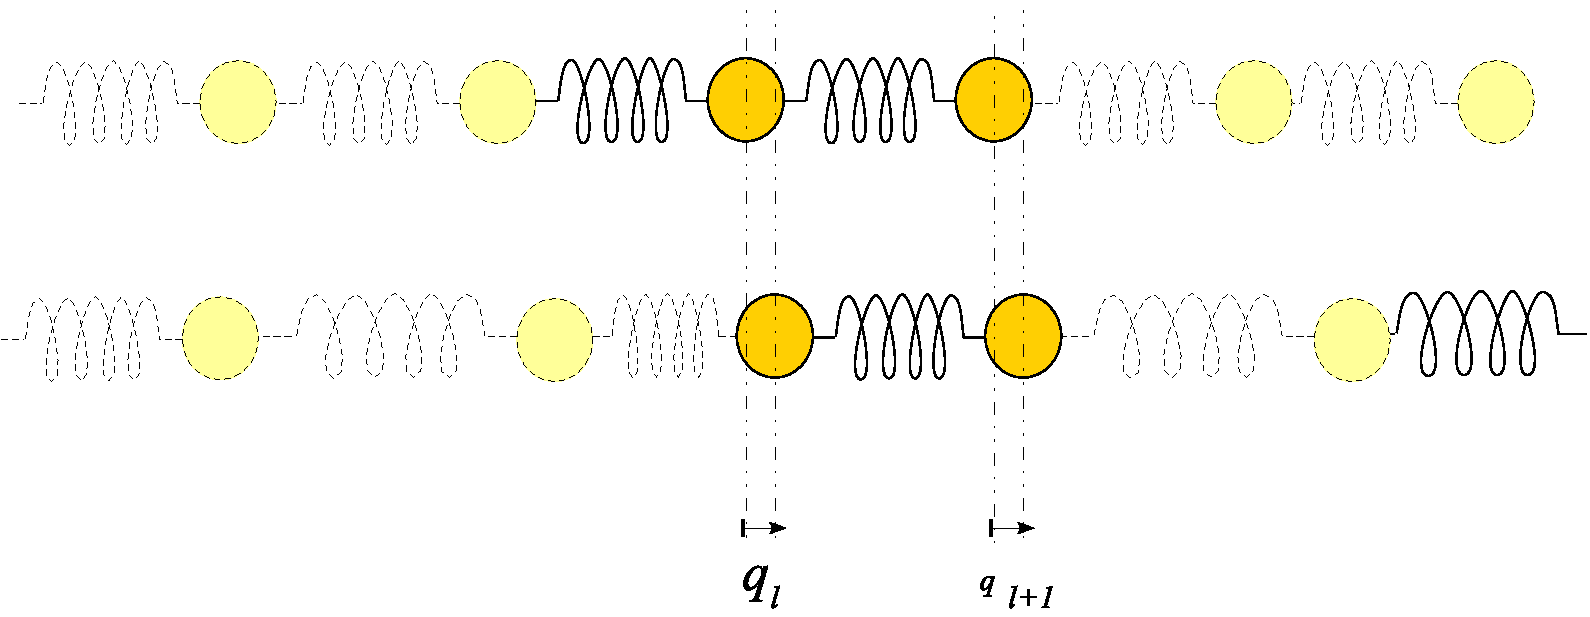
\includegraphics[height=4cm]{figs/fig-cadena.pdf}
	\caption{Cadena lineal.}
	\label{fig:cadena}
\end{figure}
La energ'ia cin'etica $T$ de este sistema est'a dada por:
\begin{equation}
T=\frac{1}{2}\sum_{l=1}^{N}m(\dot{q}^{l})^{2}(t).
\end{equation}
La energ'ia potencial $V$, que corresponde a la suma de las energ'ias
potenciales asociadas a cada una de las fuerzas arm'onicas, es
\begin{equation}
V=\frac{1}{2}\sum_{l=1}^{N}k\left\{ q^{l+1}(t) -q^{l}\left(
t\right) \right\} ^{2}.
\end{equation}
Por lo tanto, el Lagrangeano del sistema es
\begin{eqnarray}
L & = &T-V\\
& = &\frac{1}{2}\sum_{l=1}^{N}m(\dot{q}^{l})^{2}(t) -\frac{1}{2}
\sum_{l=1}^{N}k\left\{ q^{l+1}(t) -q^{l}(t)
\right\} ^{2}\\
& = &\frac{1}{2}\sum_{l=1}^{N}\left[ m(\dot{q}^{l})^{2}(t)
-k\left\{ q^{l+1}(t) -q^{l}(t) \right\}
^{2}\right].
\label{CLC}
\end{eqnarray}

\subsection{Ecuaciones de movimiento y soluci'on}
Las ecuaci'ones de movimiento de un sistema con $N$ grados de libertad pueden
ser obtenidas a partir de un lagrangeano $L=L\left(
q^{l},\dot{q}^{l}\right) $ mediante las ecuaciones de
Euler-Lagrange, esto es
\begin{equation}
\frac{\delta L}{\delta q^l}=\frac{\partial L}{\partial q^{l}}-\frac{d}{dt}\left(
\frac{\partial L}{\partial\dot{q}^{l}}\right) =0\label{EcMov1},
\end{equation}
donde hay una ecuaci'on para cada coordenada generalizada (o grado de libertad)
$q^{l}$, con $l=1,2,\dots,N$.

Considerando que para el Lagrangeano de la cadena lineal cl'asica tenemos
\begin{equation}
\frac{\partial L}{\partial\dot{q}^{l}}=m\dot{q}^l, \qquad \frac{\partial
L}{\partial q^{l}}=k(q^{l+1}-q^l)-k(q^l-q^{l-1})=k(q^{l+1}-2q^l+q^{l-1}),
\end{equation}
obtenemos que las ecuaciones de movimiento son:
\begin{equation}
\ddot{q}^l=g(q^{l+1}-2q^l+q^{l-1}).
\label{ecmovcl}
\end{equation}
Notese que hemos definido $g:=k/m$.

Para encontrar la soluci'on de las ecuaciones (\ref{ecmovcl}) es conveniente
suponer que los modos de vibraci'on de la cadena pueden ser descritos por una
onda plana. Esto est'a sugerido por la forma de la ecuaci'on (\ref{ecmovcl}),
puesto que si omitimos el primer y tercer t'ermino del miembro derecho obtenemos
la ecuaci'on del oscilador arm'onico. Adem'as, siempre podemos considerar una
expansi'on en serie de Fourier de las coordenadas generalizadas. Luego,
asumiremos una soluci'on de la forma
\begin{equation}
q^l(t)=B_k(t) e^{i\kappa l},
\label{ansatz1}
\end{equation}
donde $\kappa$ es an'alogo al n'umero de onda.

Reemplazando (\ref{ansatz1}) en (\ref{ecmovcl}) obtenemos una ecuaci'on para los
coeficientes $B_\kappa(t)$. Esta es:
\begin{equation}
\ddot{B}_\kappa(t)=g\left(e^{i\kappa}+e^{-i\kappa}
-2\right)B_\kappa(t)=-\omega_\kappa^2B_\kappa(t),
\end{equation}
es decir, una ecuaci'on tipo oscilador arm'onico para cada $\kappa$ dado, donde
la frecuencia del oscilador es
\begin{equation}
\omega_\kappa:=\sqrt{g\left(2-e^{i\kappa}-e^{-i\kappa}\right)}=2\sqrt{g}
\left|sen\frac{\kappa}{2}\right|.
\end{equation}
Por lo tanto, la soluci'on para $B_\kappa(t)$ es del tipo
\begin{equation}
B_\kappa(t)=A_\kappa e^{-i\omega_\kappa t},
\end{equation}
de modo que (\ref{ansatz1}) toma la forma
\begin{equation}
q^l(t)=A_\kappa e^{i\kappa l}e^{-i\omega_\kappa t}.
\end{equation}
Finalmente, tomando en cuenta que la ecuaci'on (\ref{ecmovcl}) es lineal en
$q^l$ y que $q^l$ es real, encontramos que la soluci'on m'as general de 
(\ref{ecmovcl}) es de la forma
\begin{equation}
q^l(t)=\sum_\kappa\left[A_\kappa e^{i\kappa l}e^{-i\omega_\kappa t}+A^*_\kappa
e^{-i\kappa l}e^{i\omega_\kappa t}\right],
\end{equation}
donde $\sum_\kappa$ denota una suma o una integral sobre $\kappa$, dependiendo
de si existen otras condiciones adicionales impuestas, como por ejemplo,
condiciones de frontera peri'odicas (cadena circular).


\section{L'imite continuo}

Reordenamos la expresi'on anterior de modo que sea m'as 'util para nuestros
prop'ositos posteriores de efectuar el l'imite al continuo. Encontramos:
\begin{eqnarray}
L & =  &\frac{1}{2}\sum_{l=1}^{N}\left[ \Delta x^{l}\frac{m}{\Delta
x^{l}}(\dot{q}^{l})^{2}(t) -\left( \Delta x^{l}\right) ^{2}k\left\{
\frac{q^{l+1}(t) -q^{l}(t) }{\Delta x^{l}
}\right\} ^{2}\right] \\
& = &\sum_{l=1}^{N}\Delta x^{l}\left[ \frac{1}{2}\frac{m}{\Delta
x^{l}}(\dot{q}^{l})^{2}(t) -\frac{1}{2}\left( \Delta x^{l}k\right)
\left\{ \left( \partial q \right) ^{l}\right\}^{2}\right] ,
\label{LagrangeanoDiscreto}
\end{eqnarray}
con
\begin{equation}
\left( \partial q\right) ^{l}=\frac{q^{l+1}-q^{l}}{\Delta x^{l}} .
\end{equation}
Por lo tanto, el lagrangiano de la cadena lineal cl'asica puede considerarse
como un caso particular de lagrangianos de la forma
\begin{equation}
L=\sum_{l=1}^{N}\Delta x^{l}{\cal L}_{l}\left( q^{l},\dot{q}^{l},\left(
\partial q\right) ^{l}\right) .\label{Lagrangeano2}
\end{equation}
Queremos encontrar la ecuaci'on de movimiento para un sistema cuyas
coordenadas generalizadas forman un s'olo conjunto de valores
continuos, es decir, el sistema posee grados de libertad continuos. Para motivar
nuestros resultados, consideraremos el sistema continuo como l'imite de un
sistema de un gran n'umero de grados de libertad.

Consideraremos un sistema discreto con interacciones "locales", es decir, que
involucren interacci'on s'olo a trav'es de pares  del tipo $ (q^{l},q^{l+1})$.
Este sistema puede ser entonces descrito por un lagrangiano de la forma:
\begin{equation}
L  =\sum_{l}\Delta x^{l}{\cal L}_{l}\left( q^{l},q^{l+1},\dot{q}^{l}\right)
=\sum_{l}\Delta x^{l}{\cal L}_{l}\left( q^{l},\dot{q}^{l},\left( \partial
q\right) ^{l}\right)  ,
\end{equation}
donde ${\cal L}_{l}\left( q^{l},\dot{q}^{l},\left( \partial q\right)^{l}\right)
$ es una cantidad que corresponde, en el l'imite continuo, a lo que
denominaremos "Densidad Lagrangeana", que incluye la informaci'on acerca de la
interacci'on entre vecinos cercanos a travez de su dependencia del t'ermino
$\left( \partial q\right) ^{l}$.

\subsection{Ecuaciones de Euler-Lagrange}\label{sec-el}
La ecuaci'on de movimiento se encuentra f'acilmente
reemplazando el Lagrangeano dado por la ecuaci'on (\ref{Lagrangeano2}) en la
ecuaci'on de movimiento (\ref{EcMov1}). En efecto:
\begin{eqnarray}
\frac{\delta L}{\delta q^l}&=&\frac{\partial}{\partial q^{l}}\left[
\sum_{m}\Delta x^{m}{\cal L}_{m}\left(
q^{m},\dot{q}^{m},\left( \partial q\right) ^{m};t\right) \right]
-\frac{d}{d t}\left( \frac{\partial}{\partial\dot{q}^{l}}\left[ \sum_{m}\Delta
x^{m}{\cal L}_{m}\left( q^{m},\dot{q}^{m},\left(\partial q\right) ^{m};t\right)
\right] \right) \\
&=&\sum_{m}\Delta x^{m}\frac{\partial}{\partial q^{l}}\left[ {\cal L}_{m}\left(
q^{m},\dot{q}^{m},\left( \partial q\right) ^{m};t\right) \right] -\sum
_{m}\Delta x^{m}\frac{d}{dt}\left( \frac{\partial}{\partial\dot{q}^{l}}\left[
{\cal L}_{m}\left( q^{m},\dot{q}^{m},\left(\partial q\right) ^{m};t\right)
\right] \right)\\
&=& \Delta x^l\frac{\partial{\cal L}_{l}}{\partial q^{l}}+\Delta
x^l\frac{\partial{\cal L}_{l}}{\partial\left( \partial q\right)
^{l}}\frac{\partial\left( \partial q\right) ^{l}}{\partial q^{l}}+\Delta
x^{l-1}\frac{\partial{\cal L}_{l-1}}{\partial\left( \partial q\right)
^{l-1}}\frac{\partial\left( \partial q\right) ^{l-1}}{\partial q^{l}}-\Delta
x^l\frac{d}{dt}\left(\frac{\partial{\cal L}_{l}}{\partial\dot{q}^{l}}\right)\\
 &=&\Delta x^l\frac{\partial{\cal L}_{l}}{\partial q^{l}}+\Delta
x^l\frac{\partial{\cal L}_{l}}{\partial\left( \partial q\right)
^{l}}\left(-\frac{1}{\Delta x^{l}}\right) +\Delta x^{l-1}\frac{\partial{\cal
L}_{l-1}}{\partial\left(
\partial q\right) ^{l-1}}\left( \frac{1}{\Delta x^{l-1}}\right)-\Delta
x^l\frac{d}{dt}\left( \frac{\partial{\cal L}_{l}}{\partial
\dot{q}^{l}}\right) \\
&=& \Delta x^l\left[\frac{\partial{\cal L}_{l}}{\partial q^{l}}-\frac{1}{\Delta
x^{l}}\left( \frac{\partial{\cal L}_{l}}{\partial\left(\partial
q\right)^{l}}-\frac{\partial{\cal L}_{l-1}}{\partial\left(\partial q\right)
^{l-1}}\right)-\frac{d}{dt}\left(\frac{\partial{\cal
L}_{l}}{\partial\dot{q}^{l}}\right)\right]  .\label{eqdisc}
\end{eqnarray}


Consideremos ahora el l'imite al continuo. En el caso de la cadena lineal, esto
significa hacer tender la separaci'on entre part'iculas a cero, es decir,
$\Delta x^{l}\rightarrow 0$ y $N\rightarrow\infty$. El sistema f'isico
resultante puede considerarse como un modelo para un ``el'astico". En este caso,
el 'indice discreto $l=1,\dots,N$ que identifica cada part'icula puede ser
reemplazado por un 'indice continuo $x$, la posici'on en equilibrio de un
elemento del el'astico. El desplazamiento $q^l(t)$ se transforma entonces en una
funci'on de $x$ y $t$, es decir en un {\em campo}, que denotaremos como
$\phi(x,t)$. En nuestro ejemplo, entonces, $\phi(x,t)$ denota el desplazamiento
en el instante $t$ del trozo de el'astico que en reposo tiene posici'on $x$. En
este l'imite tendremos que $(\partial_x q^l)\rightarrow \partial_x\phi$.
Es claro de (\ref{eqdisc}) que la ecuaci'on de movimiento para $\phi(x,t)$, en
el l'imite continuo, es
\begin{equation}
\frac{\partial{\cal L}(x,t) }{\partial \phi\left(
x,t\right) }-\frac{\partial}{\partial x}\left( \frac{\partial{\cal L}\left(
x,t\right) }{\partial\left( \partial_{x}\phi\right) }\right) -\frac{\partial
}{\partial t}\left( \frac{\partial{\cal L}(x,t) }{\partial
\dot{\phi}(x,t) }\right)  =0.\label{eccont}
\end{equation}
Finalmente, de (\ref{Lagrangeano2}) vemos que el lagrangiano de nuestro
sistema ejemplo es de la forma
\begin{equation}
L=\int dx\,{\cal L},
\end{equation}
con ${\cal L}$, la {\em densidad lagrangeana}, dada por
\begin{equation}
{\cal
L}(\phi,\dot{\phi},\partial_x\phi)=\frac{\lambda}{2}\dot{\phi}^2-\frac{Y}{2}
(\partial_x\phi)^2 , \label{lagcont}
\end{equation}
donde $\lambda=\lim_{\Delta x^l\rightarrow 0}\frac{m}{\Delta x^l}$ es la {\em
densidad lineal de masa} e $Y=\lim_{\Delta x^l\rightarrow 0} k\Delta x^l$ es el
{\em m'odulo de Young} del el'astico\footnote{Recuerde que para un sistema
lineal continuo el m'odulo de Young se define de modo que $F=YS$, donde $F$ es
la fuerza que se ejerce sobre un elemento dado del sistema (la tensi'on) y $S$
es el alargamiento por unidad de longitud del sistema. En nuestro caso
$S=\lim_{\Delta x^l\rightarrow 0}\frac{q^{l+1}(t) -q^{l}(t) }{\Delta x^{l}} $ y
la fuerza necesaria para producir ese alargamiento es $F=\lim_{\Delta
x^l\rightarrow 0}k\left(q^{l+1}(t) -q^{l}(t)\right) =\lim_{\Delta x^l\rightarrow
0}\left( \Delta x^{l}k\right) \left( \frac{q^{l+1}(t)-q^{l}(t) }{\Delta
x^{l}}\right)$.}, respectivamente. En principio $\lambda$ e $Y$ pueden variar a
lo largo del el'astico, pero aqu'i consideraremos s'olo el caso en que ellas son
constantes, es decir, el caso de un el'astico homog'eneo. Por otro lado, la
ecuaci'on del movimiento para $\phi$ es
\begin{equation}
\lambda\ddot{\phi}-Y\partial^2_x\phi=0, \label{eccontex}
\end{equation}
como puede ser verficado usando (\ref{lagcont}) y (\ref{eccont}), o efectuando
el l'imite al continuo de (\ref{ecmovcl}). La ecuaci'on (\ref{eccontex}) es
claramente una ecuaci'on de onda, con velocidad de propagaci'on
$v=\sqrt{Y/\lambda}$.

\subsection{Formalismo Hamiltoniano}
Es posible obtener una formulaci'on Hamiltoniana de sistemas continuos
en base a sistemas discretos en analog'ia a como se hizo en la
formulaci'on Lagrangeana.

Por otro lado, el momentum can'onico asociado a la coordenada generalizada $q^l$
viene dado por
\begin{equation}
p^l:=\frac{\partial L}{\partial\dot{q}^{l}}=m\dot{q}^l,
\end{equation}
de modo que, en el caso de la cadena lineal cl'asica, el Hamiltoniano del
sistema
\begin{equation}
H=T+V=\sum_l p_l \dot{q}^l-L,
\end{equation}
resulta ser
\begin{equation}
H=\sum_l \frac{1}{2m}(p_l)^2+ \frac{k}{2}\sum_l \left(q^{l+1}-q^l\right)^2.
\end{equation}

El Hamiltoniano de un sistema discreto est'a definido por 
\begin{equation}
H:=\sum_l p_{l}\dot{q}^{l}-L .
\end{equation}

En el caso en que el lagrangeano del sistema discreto es de la
forma (\ref{Lagrangeano2}), la ecuaci'on anterior puede escribirse
como
\begin{equation}
p_{l}=\Delta x^{l}\frac{\partial{\cal L}_{l}}{\partial\dot{q}^{l}},
\end{equation}
y el Hamiltoniano: 
\begin{eqnarray}
H & = &\sum_l \frac{\partial L}{\partial\dot{q}^{l}}\dot{q}^{l}-L\\
& = &\sum_{l}\Delta x^{l}\frac{\partial{\cal L}_{l}}{\partial\dot{q}^{l}}\dot
{q}^{l}-\sum_{l}\Delta x^{l}{\cal L}_{l}\\
& = &\sum_{l}\Delta x^{l}\left( \frac{\partial{\cal
L}_{l}}{\partial\dot{q}^{l}}\dot{q}^{l}-{\cal L}_{l}\right).
\end{eqnarray}
Finalmente, en el l'imite al continuo $\Delta x^{l}\rightarrow0,$ el
Hamiltoniano
se transforma en: 
\begin{equation}
H=\int dx\, {\cal H}(x,t) \label{HamiltonianoTotal} ,
\end{equation}
donde hemos definido 
\begin{eqnarray}
{\cal H}(x,t) & := &\pi(x,t) \dot{\phi}(x,t)-{\cal L}(x,t) ,\\
\pi(x,t) & := &\frac{\partial{\cal L}}{\partial\dot{\phi}}.
\end{eqnarray}
como  la densidad Hamiltoniana y la densidad de momento can'onico conjugado,
respectivamente. Note que, para un campo $\phi$ general, el ``momentum can'onico
total'' $P:=\int dx\, \pi$ no coincide necesariamente con el \textit{momentum
lineal} del sistema.



\subsection{Cadena Lineal: Modelo continuo  (el el'astico!)}\label{seccon}

Si asumimos que nuestro ``el'astico"\ tiene extensi'on infinita (tal como el
campo
electromagn'etico que pretendemos cuantizar m'as adelante), es decir, $x\in
(-\infty,\infty)$, entonces la soluci'on de (\ref{eccontex}) puede ser expandida
en serie
de Fourier de la forma
\begin{equation}
\phi(x,t) =\int_{-\infty}^{+\infty} dk\left\{ B_k(t) e^{ikx}
+B_k^{\ast}(t) e^{-ikx}\right\} .\label{q1}
\end{equation}

Para determinar los $B_k(t) $  podemos reemplazar
la ecuaci'on (\ref{q1}) en (\ref{eccontex}), teniendo en cuenta que
\begin{eqnarray}
\frac{\partial^{2}\phi(x,t) }{\partial x^{2}} & = &\int_{-\infty}^{+\infty}
dk\left\{
-k^{2}B_k(t) e^{ikx}+\text{c.c.}\right\}, \\
\ddot{\phi}(x,t)& = &\int_{-\infty}^{+\infty} dk\left\{\ddot{B}_k(t)
e^{ikx}+\text{c.c.}\right\} .
\end{eqnarray}
Aqu'i c.c. denota el complejo conjugado de la expresi'on anterior. Luego, obtenemos
\begin{equation}
\frac{1}{v^{2}}\ddot{B}_k(t) =-k^{2}B_k(t) ,
\end{equation}
que es una ecuaci'on diferencial tipo oscilador harm'onico para $B_k(t)$, cuya
soluci'on es de la forma:
\begin{equation}
B_k(t) =\alpha_ke^{-i\omega_kt}+\beta_ke^{+i\omega_kt} ,\qquad \omega_k=v|k| ,
\end{equation}
que corresponden a ondas que se propagan con frecuencia $\omega_k$. De este
modo, la soluci'on es
\begin{eqnarray}
\phi(x,t) &=&\int_{-\infty}^{+\infty} dk\left\{ \left(
\alpha_ke^{-i\omega_kt}+\beta_ke^{+i\omega_kt}\right)  e^{ikx}+\left(
\alpha^*_ke^{+i\omega_kt}+\beta^*_ke^{-i\omega_kt}\right)  e^{-ikx}\right\} \\
&=&\int_{-\infty}^{+\infty} dk\left\{\left(\alpha_ke^{ikx}
+\beta^*_ke^{-ikx}\right) e^{-i\omega_kt}
+\left(\alpha^*_ke^{-ikx} +\beta_ke^{ikx}\right) e^{+i\omega_kt}\right\}\\
&=&\int_{-\infty}^{+\infty} dk\left\{\left(\alpha_ke^{ikx}
+\beta^*_{-k}e^{ikx}\right) e^{-i\omega_kt}
+\left(\alpha^*_ke^{-ikx} +\beta_{-k}e^{-ikx}\right) e^{+i\omega_kt}\right\}\\
&=&\int_{-\infty}^{+\infty} dk\left\{\left(\alpha_k +\beta^*_{-k}\right)
e^{-i\omega_kt} e^{ikx}
+\left(\alpha^*_k +\beta_{-k}\right) e^{+i\omega_kt}e^{-ikx}\right\}\\
&=&\int_{-\infty}^{+\infty} dk\left\{\gamma_k\, e^{-i\omega_kt} e^{ikx}
+\gamma_k^*\, e^{+i\omega_kt}e^{-ikx}\right\}\\
&=&\int_{-\infty}^{+\infty} dk\left\{B_k(t) e^{ikx}+B_k^*(t)e^{-ikx}\right\},
\label{soll}
\end{eqnarray}
donde $B_k(t):=\gamma_k\, e^{-i\omega_kt}$  con las constantes arbitrarias
$\gamma_k:=\alpha^*_k +\beta_{-k}$. La densidad de momento can'onico la podemos
calcular mediante su
definici'on (\ref{DensidadMomentoCanonicoConjugado}): 
\begin{eqnarray}
\pi(x,t) & = &\frac{\partial{\cal L}(x,t)}{\partial\dot{\phi}(x,t) }\\
& = &\lambda\dot{\phi}(x,t) \\
& = &\lambda\int_{-\infty}^{+\infty} dk\left\{ \dot{B}_k(t)
e^{ikx}+\dot{B}_k^{\ast
}(t) e^{-ikx}\right\}  \\
& = &\lambda\int_{-\infty}^{+\infty} dk\left\{ -i\omega_kB_k(t) e^{ikx}+i\omega
_kB_k^{\ast}(t) e^{-ikx}\right\} \\
& = &i\lambda\int_{-\infty}^{+\infty} dk\,\omega_k\left\{ -B_k(t)
e^{ikx}+B_k^{\ast
}(t) e^{-ikx}\right\}. \label{Pi1} 
\end{eqnarray}
Por lo tanto, el momento can'onico total es
\begin{eqnarray}
\Pi & = &\int_{-\infty}^{+\infty} dx\,\pi(x,t) \\
& = &\int_{-\infty}^{+\infty} dx\left[ i\lambda\int dk\,\omega_k\left\{ -B_k(t)
e^{ikx}+B_k^{\ast}(t) e^{-ikx}\right\} \right] \\
& = &i\lambda\int_{-\infty}^{+\infty} dk\,\omega_k\left\{ -B_k(t) \left(
\int_{-\infty}^{+\infty}
dx\, e^{ikx}\right) +B_k^{\ast}(t) \left( \int_{-\infty}^{+\infty} dx\,
e^{-ikx}\right) \right\}  \\
& = &i\lambda\int_{-\infty}^{+\infty} dk\,\omega_k\left\{ -B_k(t)\,
2\pi\delta(k) +B_k^{\ast}(t)\, 2\pi\delta(k)\right\} \\
& = &2\pi i\lambda\int_{-\infty}^{+\infty} dk\,\omega_k\left\{ -B_k(t)
+B_k^{\ast}(t) \right\} \delta(k) \\
& = &2\pi i\,\lambda\omega_{0}\left\{ -B_{0}(t) +B_{0}^{\ast}(t) \right\}\\
& = &0 .
\end{eqnarray}
 En el c'alculo anterior, hemos usado $\int_{-\infty}^{+\infty} dx\,e^{\pm
ikx}=2\pi\delta\left(
k\right)$ y $\omega_{0}=0$. Por otro lado, evaluamos la densidad Hamiltoniana:
\begin{eqnarray}
{\cal H} & = &\pi(x,t) \dot{\phi}(x,t) -{\cal L}(x,t) \\
& = &\left\{ \lambda\dot{\phi} \right\} \dot{\phi} -\left\{
\frac{1}{2}\lambda\dot{\phi}^{2} -\frac{1}{2}Y\left( \partial_{x}\phi\right)
^{2}\right\} \\
& = &\lambda\dot{\phi}^{2} -\frac{1}{2}\lambda\dot{\phi}^{2} +\frac{1}{2}Y\left(
\partial_{x}\phi\right) ^{2}\\
& = &\frac{1}{2}\lambda\dot{\phi}^{2} +\frac{1}{2}Y\left(\partial_{x}\phi\right)
^{2}\\
& = &\frac{1}{2}\left[\lambda\left\{ i\int dk\,\omega_k\left( -B_k(t)
e^{ikx}+B_k^{\ast}(t) e^{-ikx}\right) \right\} \left\{ i\int
dk'\omega_{k'}\left(-B_{k'}(t) e^{ik'x}+B_{k'}^{\ast}(t)
e^{-ik'x}\right) \right\}\right. \nonumber \\
&&\left.+Y\left\{ i\int dk\left( B_k(t) e^{ikx}-B_k^{\ast}(t) e^{-ikx}\right)
k\right\} \left\{ i\int dk'\left( B_{k'}(t)e^{ik'x}-B_{k'}^{\ast}(t)
e^{-ik'x}\right) k'\right\}\right] \\
& = &-\frac{1}{2}\iint dk\,dk'\left( \lambda\omega_k\omega_{k'}+Ykk'\right)
\left[e^{i\left( k+k' \right) x} B_k(t) B_{k'}(t)+e^{-i\left( k+k' \right)
x}B_k^{\ast}(t) B_{k'}^{\ast}(t)  \right.\nonumber \\
&&\left.-e^{i(k-k') x} B_k(t) B_{k'}^{\ast}(t)-e^{-i\left( k-k' \right)
x}B_k^{\ast}(t) B_{k'}(t) \right],
\end{eqnarray}
entonces el Hamiltoniano total es
\begin{eqnarray}
H & = &\int dx\, {\cal H}(x,t) \\
& = &-\frac{1}{2}\iiint dx\,dk\,dk'\left( \lambda\omega_k\omega_{k'}+gkk'\right)
\left[e^{i\left( k+k' \right) x} B_k(t) B_{k'}(t) \right.\nonumber \\
&&\left.+e^{-i\left( k+k' \right) x}B_k^{\ast}(t) B_{k'}^{\ast}(t) -e^{i(k-k')
x} B_k(t) B_{k'}^{\ast}(t)-e^{-i\left( k-k' \right) x}B_k^{\ast}(t) B_{k'}(t)
\right]\\
& = &-\pi\int dk\left[\left( \lambda\omega_k\omega_{-k}+Yk(-k)\right)\left(
B_k(t) B_{-k}(t)+B_k^{\ast}(t) B_{-k}^{\ast}(t) \right) \right.\nonumber \\
&&\left.-\left( \lambda\omega_k\omega_k+Ykk\right)\left( B_k(t)
B_k^{\ast}(t)+B_k^{\ast}(t) B_k(t) \right)\right]\\
& = &-\pi\int dk\left[\left( \lambda\omega_k^2-Yk^2\right)\left( B_k(t)
B_{-k}(t)+B_k^{\ast}(t) B_{-k}^{\ast}(t) \right) \right.\nonumber \\
&&\left.-\left( \lambda\omega_k^2+Yk^2\right)\left( B_k(t)
B_k^{\ast}(t)+B_k^{\ast}(t) B_k(t) \right)\right]\\
& = &+4\pi\lambda\int dk\, \omega_k^2\, B_k(t) B_k^{\ast}(t),
\end{eqnarray}
donde hemos usado $\int_{-\infty}^{+\infty} dx\,e^{\pm
i(k-k')x}=2\pi\delta\left(
k-k'\right)$  y $\lambda\omega_k^2=Yk^2$.

Por otro lado, la densidad de momentum lineal del sistema es
\begin{eqnarray}
p^{x}&=&-\frac{\partial\mathcal{L}}{\partial\dot{\phi}}\partial_{x}\phi\\
&=&-\left[  i\lambda\int dk\omega_k\left\{  -B_k\left(  t\right)
e^{ikx}+B_k^{\ast}\left(  t\right)  e^{-ikx}\right\}  \right]  \left[  i\int
dk^{\prime}k^{\prime}\left\{  B_{k^{\prime}}\left(  t\right)
e^{ik^{\prime}x}-B_{k^{\prime}}^{\ast}\left(  t\right)
e^{-ik^{\prime}x}\right\}  \right]\\
&=&\lambda\int\int dkdk^{\prime}\omega_kk^{\prime}\left\{  -B_k\left(t\right)
e^{ikx}+B_k^{\ast}\left(  t\right)  e^{-ikx}\right\}
\left\{B_{k^{\prime}}\left(  t\right)
e^{ik^{\prime}x}-B_{k^{\prime}}^{\ast}\left(
t\right)  e^{-ik^{\prime}x}\right\} \\
&=&\lambda\int\int dkdk^{\prime}\omega_kk^{\prime}\left\{
-B_kB_{k^{\prime}}e^{i\left(  k+k^{\prime}\right)
x}+B_kB_{k^{\prime}}^{\ast}e^{i\left(  k-k^{\prime}\right)  x}\right. \\
&&\left.  +B_k^{\ast}B_{k^{\prime}}e^{-i\left(  k-k^{\prime}\right)
x}-B_k^{\ast}B_{k^{\prime}}^{\ast}e^{-i\left(  k+k^{\prime}\right)  x}\right\}\\
&=&-\lambda\int\int dkdk^{\prime}\omega_kk^{\prime}\left\{
B_kB_{k^{\prime}}e^{i\left(  k+k^{\prime}\right)
x}-B_kB_{k^{\prime}}^{\ast}e^{i\left(k-k^{\prime}\right)  x}\right. \\
&&\left.  -B_k^{\ast}B_{k^{\prime}}e^{-i\left(  k-k^{\prime}\right)
x}+B_k^{\ast}B_{k^{\prime}}^{\ast}e^{-i\left(  k+k^{\prime}\right)x}\right\}  ,
\end{eqnarray}
de modo que el momentum lineal total es
\begin{eqnarray}
P^{x}&=&\int dx\text{ }p_{x}\\
&=&-\lambda\int\int\int
dxdkdk^{\prime}\omega_kk^{\prime}\left\{B_kB_{k^{\prime}}e^{i\left(
k+k^{\prime}\right)  x}-B_kB_{k^{\prime}}^{\ast}e^{i\left(  k-k^{\prime}\right)
x}\right.\nonumber\\
&&\left.-B_k^{\ast}B_{k^{\prime}}e^{-i\left(  k-k^{\prime}\right)
x}+B_k^{\ast}B_{k^{\prime}}^{\ast
}e^{-i\left(  k+k^{\prime}\right)  x}\right\} \\
&=&-2\pi\lambda\int\int dkdk^{\prime}\omega_kk^{\prime}\left\{
B_kB_{k^{\prime}}\delta\left( k+k^{\prime}\right)
-B_kB_{k^{\prime}}^{\ast}\delta\left(  k-k^{\prime}\right)\right.\nonumber\\
&&\left.-B_k^{\ast}B_{k^{\prime}}\delta\left(k-k^{\prime}\right)
+B_k^{\ast}B_{k^{\prime}}^{\ast}\delta\left(k+k^{\prime}\right)  \right\} \\
&=&-2\pi\lambda\left\{  \int dk\omega_k\left(  -k\right)  B_kB_{-k}-\int
dk\omega_kkB_kB_k^{\ast}\right. \\
&&\left.  -\int dk\omega_kkB_k^{\ast}B_k+\int dk\omega_k\left(-k\right)
B_k^{\ast}B_{-k}^{\ast}\right\} \\
&=&2\pi\lambda\left\{  \int dk\omega_kk\left(
B_kB_{-k}+B_k^{\ast}B_{-k}^{\ast}\right)  +\int dk\omega_kk\left(
B_kB_k^{\ast}+B_k^{\ast}B_k\right)  \right\}\\
&=&4\pi\lambda\int dk\omega_kkB_kB_k^{\ast}.
\end{eqnarray}
\subsection{Cadena Lineal Cu'antica}\label{seccon}

Para cuantizar el sistema, $q(x,t) $ y $\pi(x,t) $ deben ser operadores (de
campo), que satisfagan relaciones de conmutaci'on no triviales. Pero,
\textquestiondown qu'e forma deben tener estas relaciones?. Para resolver esta
pregunta, consideraremos el l'imite continuo de las  (conocidas) relaciones de
conmutaci'on que se aplican a un sistema discreto.

Un sistema discreto, como el descrito por un lagrangiano de la forma
(\ref{Lagrangeano2}), es cuantizado usualmente elevando las variables de
configuraci'on $q^l$ y sus momenta can'onicos $p_l$ a la calidad de operadores
$\hat{q}^l$ y $\hat{\pi}_l$, que act'uan sobre un espacio de Hilbert
\begin{equation}
{\cal H}_{\{q\}}:={\cal H}_{q^1}\otimes{\cal H}_{q^2}\otimes \cdots \otimes
{\cal H}_{q^N}=\prod_l {\cal H}_{q^l},
\end{equation}
y que satisfacen las relaciones de conmutaci'on can'onicas:
\begin{eqnarray}
\left[ \hat{q}^l, \hat{p}_m\right] &=&i\hbar\, \delta^l_m \hat{1},\\
\left[ \hat{q}^l, \hat{q}^m\right] &=&0,\\
\left[\hat{p}_l , \hat{p}_m\right] &=&0.
\end{eqnarray}
Para los modelos descritos por  (\ref{Lagrangeano2}), $p_{l}=\Delta
x^{l}\frac{\partial{\cal L}_{l}}{\partial\dot{q}^{l}}$ ($l$ fijo), de modo que
\begin{equation}
\left[ \hat{q}^l,\frac{\partial\hat{\cal L}_{m}}{\partial\dot{q}^{m}}\right]
=i\hbar\, \frac{\delta^l_m}{\Delta x^{m}} \hat{1}.
\label{rccd}
\end{equation}

En el l'imite continuo que estamos considerando ($\Delta x^l\rightarrow 0$,
$N\rightarrow\infty$, $l\rightarrow x$, $m\rightarrow x'$), vemos que la
relaci'on de conmutaci'on (\ref{rccd}) tiende a
\begin{eqnarray}
\left[ \hat{\phi}(x,t),\hat{\pi}(x',t)\right] &=&i\hbar\, \delta (x-x') \hat{1}.
\label{rccc}\\
\left[ \hat{\phi}(x,t),\hat{\phi}(x',t)\right]&=&0,\\
\left[ \hat{\pi}(x,t),\hat{\pi}(x',t)\right]&=&0 \label{rccc3}.
\end{eqnarray}
Donde ahora $\hat{\phi}(x)$ y $\hat{\pi}(x')$ son \textit{operadores de campo}
(es decir, un campo de operadores, u  operadores distintos definidos en cada
punto del espacio) que act'uan sobre un espacio de Hilbert ${\cal H}_\phi$ que,
formalmente, es un producto infinito y continuo de los espacios de Hilbert
${\cal H}_{\phi(x)}$ asociados a cada grado de libertal $\phi(x)$ ($x$ fijo) del
campo:
\begin{equation}
{\cal H}_\phi:=\prod_x {\cal H}_{\phi(x)}=\lim_{\Delta x^l \rightarrow 0, N
\rightarrow\infty} {\cal H}_{\{q\}}.
\end{equation}

Que el lado derecho de (\ref{rccd}) tiende efectivamente a una delta de Dirac
puede verificarse considerando que
\begin{eqnarray}
\int dx'\lim_{\Delta x^l \rightarrow 0}\left( \frac{\delta^l_m}{\Delta
x^{m}}\right) f(x')&=& \lim_{\Delta x^l \rightarrow 0}\sum_m \Delta x^m\left(
\frac{\delta^l_m}{\Delta x^{m}}\right) f(m) \nonumber \\
&=&\lim_{\Delta x^l \rightarrow 0}\sum_m \delta^l_m f(m) = \lim_{\Delta x^l
\rightarrow 0} f(l) \nonumber \\
&=& f(x),
\end{eqnarray}
para una funci'on arbitraria $f$.

Las relaciones de conmutaci'on  (\ref{rccc})-(\ref{rccc3}) ser'an entonces las
relaciones de conmutaci'on can'onicas para un sistema descrito por un campo
$\phi$. No es dificil verificar que en el caso m'as general de un sistema con
m'as
campos definidos en un espacio tridimensional, ver (\ref{lag4d}), las relaciones
de conmutaci'on can'onicas a usar para los operadores de campo son
\begin{eqnarray}
\left[ \hat{\phi}^A(\vec{x},t),\hat{\pi}^B(\vec{x}',t)\right] &=&i\hbar\,
\delta^{AB}\delta^{(3)} (\vec{x}-\vec{x}') \hat{1},\label{rccc4d}\\
\left[ \hat{\phi}^A(\vec{x},t),\hat{\phi}^B(\vec{x}',t)\right] &=&0,\\
\left[ \hat{\pi}^A(\vec{x},t),\hat{\pi}^B(\vec{x}',t)\right] &=&0.
\end{eqnarray}
donde $\delta^{(3)} (\vec{x}-\vec{x}') $ es la correspondiente delta de Dirac
tridimensional\footnote{Definida de modo que $\int \delta^{(3)}
(\vec{x}-\vec{x}') f(\vec{x}')\, dV=f(\vec{x})$ para toda funci'on
$f(\vec{x})$.}.

Finalmente, la din'amica del sistema est'a determinada por el operador
Hamiltoniano $\hat H$ a trav'es de la ecuaci'on (cuadro de Schr\"odinger):
\begin{equation}
 i\hbar\, \partial_t\left|\Psi\right>={\hat H}\left|\Psi\right>
\end{equation}
o, equivalentemente (cuadro de Heisenberg) por la evoluci'on de un operador
cualquiera $\hat O$ por medio de
\begin{equation}
i\hbar\, \partial_t{\hat O}=\left[{\hat O},{\hat H}\right].
\end{equation}

\subsection{Ecuaci'on de movimiento para el operador $\hat{\phi}(x)$}

Si ahora $\hat{\phi}(x) $ y $\hat{\pi}(x) $ son operadores de campo, entonces su
din'amica viene dada por la ecuaci'on de movimiento de Heisenberg (cuadro de
Heisenberg!):
\begin{eqnarray}
\dot{\hat{\phi}}(x,t) & = &-\frac{i}{\hbar}\left[ \hat{\phi}(x,t)
,\hat{H}\right] , \label{evPI1}\\
\dot{\hat{\pi}}(x,t) & = &-\frac{i}{\hbar}\left[\hat{\pi}(x,t),\hat{H} \right]
\label{evPI} .
\end{eqnarray}

En nuestro sistema ejemplo, el hamiltoniano es $\hat{H}=\int dx\left\{
\frac{1}{2\lambda}\left[ \hat{\pi}(x,t)\right]^2 +\frac{Y}{2}\left[ \partial_x
\hat{\phi} (x,t)\right]^2 \right\}$.
As'i, (\ref{evPI1}) toma la forma
\begin{eqnarray}
\dot{\hat{\phi}}(x,t) & = &-\frac{i}{\hbar}\left[ \hat{\phi}(x,t)
,\hat{H}\right] \\
 & = &-\frac{i}{\hbar}\left[ \hat{\phi}(x,t) ,\int dx'\left\{
\frac{1}{2\lambda}\left[ \hat{\pi}(x',t)\right]^2 +\frac{Y}{2}\left[
\partial_{x'} \hat{\phi} (x',t)\right]^2 \right\}\right]  \\
 & = &-\frac{i}{\hbar}\int dx'\left[ \hat{\phi}(x,t) , \frac{1}{2\lambda}\left[
\hat{\pi}(x',t)\right]^2 +\frac{Y}{2}\left[ \partial_{x'} \hat{\phi}
(x',t)\right]^2\right] \\
 & = &-\frac{i}{\hbar}\int dx'\left\{\frac{1}{2\lambda}\left[ \hat{\phi}(x,t) ,
\left[ \hat{\pi}(x',t)\right]^2\right] +\frac{Y}{2}\left[ \hat{\phi}(x,t) ,
\left[ \partial_{x'} \hat{\phi} (x',t)\right]^2\right] \right\}\\
 & = &-\frac{i}{\hbar}\int dx'\left\{\frac{1}{2\lambda}\left[ \hat{\phi}(x,t) ,
\left[ \hat{\pi}(x',t)\right]^2\right] +\frac{Y}{2}\partial_{x'}\left[
\hat{\phi}(x,t) , \left[  \hat{\phi} (x',t)\right]^2\right] \right\} \\
 & = &-\frac{i}{\hbar}\int dx'\left\{\frac{1}{2\lambda}\left[ \hat{\phi}(x,t) ,
\left[ \hat{\pi}(x',t)\right]^2\right]  \right\}\\
 & = &-\frac{i}{2\hbar\lambda}\int dx'\left\{\hat{\pi}(x',t)\left[
\hat{\phi}(x,t) , \hat{\pi}(x',t)\right] +\left[ \hat{\phi}(x,t) ,
\hat{\pi}(x',t)\right]\hat{\pi}(x',t)  \right\}\\
 & = &\frac{1}{2\lambda}\int dx'\left\{\hat{\pi}(x',t)\delta (x-x') +\delta
(x-x') \hat{\pi}(x',t)  \right\}\\
 & = &\frac{1}{\lambda}\int dx'\,\hat{\pi}(x',t)\delta (x-x') \\
 & = &\frac{1}{\lambda}\hat{\pi}(x,t).
\end{eqnarray}
Por otro lado, (\ref{evPI}) implica que
\begin{eqnarray}
\dot{\hat{\pi}}(x) & = &-\frac{i}{\hbar}\left[\hat{\pi}(x),\hat{H} \right] \\
& = &-\frac{i}{\hbar}\left[\hat{\pi}(x), \int dx'\left\{
\frac{1}{2\lambda}\left[ \hat{\pi}(x',t)\right]^2 +\frac{Y}{2}\left[
\partial_{x'} \hat{\phi} (x',t)\right]^2 \right\}\right]\\
& = &-\frac{i}{\hbar}\int dx'\left[\hat{\pi}(x), \frac{1}{2\lambda}\left[
\hat{\pi}(x',t)\right]^2 +\frac{Y}{2}\left[ \partial_{x'} \hat{\phi}
(x',t)\right]^2 \right]\\
& = &-\frac{i}{\hbar}\int dx'\left[\hat{\pi}(x), \frac{Y}{2}\left[ \partial_{x'}
\hat{\phi} (x',t)\right]^2 \right]\\
& = &-\frac{iY}{2\hbar}\int dx'\left[\hat{\pi}(x), \left[ \partial_{x'}
\hat{\phi}(x',t)\right]^2 \right]\\
& = &-\frac{iY}{2\hbar}\int dx'\left\lbrace \partial_{x'} \hat{\phi}
(x',t)\left[\hat{\pi}(x),  \partial_{x'} \hat{\phi} (x',t)\right]
+\left[\hat{\pi}(x),  \partial_{x'} \hat{\phi} (x',t)\right]\partial_{x'}
\hat{\phi} (x',t)\right\} \\
& = &-\frac{iY}{2\hbar}\int dx'\left\{ \partial_{x'} \hat{\phi}
(x',t)\partial_{x'}\left[\hat{\pi}(x),   \hat{\phi} (x',t)\right]
+\partial_{x'}\left[\hat{\pi}(x),  \hat{\phi} (x',t)\right]\partial_{x'}
\hat{\phi} (x',t)\right\} \\
& = &-\frac{Y}{2}\int dx'\left\{ \partial_{x'} \hat{\phi}
(x',t)\partial_{x'}\delta(x-x') +\partial_{x'}\delta(x-x')\partial_{x'}
\hat{\phi} (x',t)\right\}\\
& = &-Y\int dx' \partial_{x'} \hat{\phi} (x',t)\partial_{x'}\delta (x-x') \\
& = &Y\int dx' \partial^2_{x'} \hat{\phi} (x',t)\delta (x-x') \\
& = &Y\partial^2_{x} \hat{\phi} (x,t).
\end{eqnarray}
En resumen, las ecuaciones de evoluci'on para los operadores de campo son:
\begin{equation}
\dot{\hat{\phi}}(x,t)=\frac{1}{\lambda}\hat{\pi}(x,t), \label{eephi}
\end{equation}
\begin{equation}
\dot{\hat{\pi}}(x) =Y\partial^2_{x} \hat{\phi} (x,t).\label{eepi}
\end{equation}
Derivando (\ref{eephi}) con respecto al tiempo y usando  (\ref{eepi})
encontramos
 \begin{equation}
\ddot{\hat{\phi}}(x,t)=\frac{1}{\lambda}\dot{\hat{\pi}}(x,t)=\frac{Y}{\lambda}
\partial^2_{x} \hat{\phi} (x,t) ,
\end{equation}
es decir, el operador de campo $\hat\phi$ satisface la misma ecuaci'on de onda
que su an'alogo cl'asico, ver  (\ref{eccontex}).
Como consecuencia, la mismas expansiones cl'asicas (\ref{q1}) y (\ref{Pi1}) son
v'alidas en el caso cuantizado, s'olo que ahora $\phi$ y $\pi$ y por lo tanto
$B_k(t) $ y $B_k^{\ast}(t) $ deben ser operadores.


\subsection{Cantidades Importantes}

De la secci'on anterior vemos que podemos escribir (\ref{q1}) como el operador:
\begin{equation}
\hat{\phi}(x,t) =\int_{-\infty}^\infty dk\left\{ \hat{B}_k(t)
e^{ikx}+\hat{B}_k^\dagger (t) e^{-ikx}\right\},
\label{qOperador1}
\end{equation}
con $\dot{\hat{B}}_k(t)=-i\omega_k\hat{B}_k(t)$, $\omega_k=v|k|$, que nos
dice que nuestro campo est'a constituido por una superposici'on
infinita de ondas planas, cada una para un valor distinto del n'umero de
onda $k$.
Tambi'en se tiene que la densidad de momento conjugado (\ref{Pi1}) se puede
escribir como
\begin{equation}
\hat{\pi}(x,t) =i\lambda\int_{-\infty}^\infty dk\,\omega_k\left\{
-\hat{B}_k(t) e^{ikx}+\hat{B}_k^\dagger (t)
e^{-ikx}\right\}.\label{piOperador1}
\end{equation}

Debido a que los operadores de campo satisfacen las relaciones de conmutaci'on
(\ref{rccc}), los operadores
$\hat{B}_k(t) $ y $\hat{B}_k^\dagger (t) $ tambi'en satisfacer'an relaciones
de conmutaci'on no triviales.

Para determinar estas relaciones, escribiremos primero $\hat{B}_k(t) $ y
$\hat{B}_k^\dagger (t) $ en funci'on de $\hat{\phi}(x,t) $ y $\hat{\pi}(x,t) $.
En efecto, reescribiendo $\hat{\phi}(x,t) $ de la siguiente forma: 
\begin{eqnarray}
\hat{\phi}(x,t) & = &\int_{-\infty}^{\infty} dk\left\{
\hat{B}_k(t)e^{ikx}+\hat{B}_k^\dagger (t) e^{-ikx}\right\} \\
& = &\int_{-\infty}^{\infty}dk\hat{B}_k(t)
e^{ikx}+\int_{-\infty}^{\infty}dk\hat{B}_k^\dagger (t) e^{-ikx}\\
& = &\int_{-\infty}^{\infty}dk\hat{B}_k(t)
e^{ikx}+\int_{\infty}^{-\infty}\left( -dk\right) \hat{B}_{-k}^\dagger (t)
e^{-i( -k) x}\\
& = &\int_{-\infty}^{\infty}dk\hat{B}_k(t)
e^{ikx}-\int_{\infty}^{-\infty}dk\hat{B}_{-k}^\dagger (t) e^{ikx}\\
& = &\int_{-\infty}^{\infty}dk\hat{B}_k(t)
e^{ikx}-\left(-\int_{-\infty}^{\infty}dk\hat{B}_{-k}^{\dagger}(t)e^{ikx}\right)\\
& = &\int_{-\infty}^{\infty}dk\hat{B}_k(t) e^{ikx}+\int
_{-\infty}^{\infty}dk\hat{B}_{-k}^\dagger (t) e^{ikx} \\
& = &\int dk\left\{ \hat{B}_k(t) e^{ikx}+\hat{B}_{-k}^\dagger (t)
e^{ikx}\right\} \\
& = &\int dk\,e^{ikx}\left\{ \hat{B}_k(t) +\hat{B}_{-k}^\dagger \left(
t\right) \right\} ,\label{qOperador2} 
\end{eqnarray}
obtenemos:
\begin{eqnarray}
\int dx\,e^{-ik'x}\hat{\phi}(x,t)  & = &\iint dk\,dx\,e^{i(k-k') x}\left\{
\hat{B}_k(t) +\hat{B}_{-k}^\dagger (t) \right\} \\
& = &2\pi\int dk\left\{ \hat{B}_k\left(t\right) +\hat{B}_{-k}^\dagger (t)
\right\} \delta(k-k') \\
& = &2\pi\left\{ \hat{B}_{k'}(t) +\hat{B}_{-k'}^\dagger (t) \right\} .
\end{eqnarray}
Por lo tanto, tenemos que
\begin{equation}
\hat{B}_{k'}(t) +\hat{B}_{-k'}^\dagger (t)  = \frac{1}{2\pi}\int
dx\,e^{-ik'x}\hat{\phi}(x,t) \label{Rel1}.
\end{equation}
De igual manera con (\ref{piOperador1}):
\begin{eqnarray}
\hat{\pi}(x,t) & = &i\lambda\int_{-\infty}^{\infty} dk\,\omega_k\left\{
-\hat{B}_k(t) e^{ikx}+\hat{B}_k^\dagger (t)
e^{-ikx}\right\} \\
& = &-i\lambda\int_{-\infty}^{\infty}dk\,\omega_k\hat{B}_k(t)
e^{ikx}+i\lambda\int_{-\infty}^{\infty}dk\,\omega_k\hat{B}_k^\dagger \left(
t\right) e^{-ikx}\\
& = &-i\lambda\int_{-\infty}^{\infty}dk\,\omega_k\hat{B}_k(t)
e^{ikx}+i\lambda\int_{\infty}^{-\infty}\left( -dk\right) \omega_{-k}\hat
{B}_{-k}^\dagger (t) e^{-i( -k) x}\\
& = &-i\lambda\int_{-\infty}^{\infty}dk\,\omega_k\hat{B}_k(t)
e^{ikx}-i\lambda\int_{\infty}^{-\infty}dk\,\omega_k\hat{B}_{-k}^\dagger \left(
t\right) e^{ikx}\\
& = &-i\lambda\int_{-\infty}^{\infty}dk\,\omega_k\hat{B}_k(t)
e^{ikx}-i\lambda\left( -\int_{-\infty}^{\infty}dk\,\omega_k\hat{B}_{-k} 
^\dagger (t) e^{ikx}\right) \\
& = &-i\lambda\int_{-\infty}^{\infty}dk\,\omega_k\hat{B}_k(t)
e^{ikx}+i\lambda\int_{-\infty}^{\infty}dk\,\omega_k\hat{B}_{-k}^\dagger \left(
t\right) e^{ikx}\\
& = &i\lambda\int dk\,\omega_ke^{ikx}\left\{ -\hat{B}_k(t)
+\hat{B}_{-k}^\dagger (t) \right\} ,\label{piOperador2}
\end{eqnarray}
encontramos
\begin{eqnarray}
\int dx\,e^{-ik'x}\hat{\pi}(x,t) & = &i\lambda\int dk\,\omega_k\int
dxe^{i\left(
k-k'\right) x}\left\{ -\hat{B}_k(t) +\hat{B}_{-k}^\dagger (t) \right\} \\
& = &2\pi i\lambda\int dk\,\omega_k\left\{
-\hat{B}_k(t) +\hat{B}_{-k}^\dagger (t)\right\} \delta(k-k') \\
& = &2\pi i\lambda\omega_{k'}\left\{ -\hat{B}_{k'}(t) +\hat{B}_{-k'}^\dagger (t)
\right\}.
\end{eqnarray}
De aqu'i encontramos que
\begin{equation}
\hat{B}_{k'}(t) -\hat{B}_{-k'}^\dagger (t)  =
\frac{i}{2\pi\lambda\omega_{k'}}\int dx\, e^{-ik'x}\hat{\pi}(x,t) .\label{Rel2}
\end{equation}
Sumando (\ref{Rel1}) y (\ref{Rel2}) podemos despejar el operador $\hat{B}_{k'}$:
\begin{equation}
\hat{B}_{k'}(t)  = \frac{1}{4\pi}\int dx\, e^{-ik'x}\left( \hat{\phi}(x,t)
+\frac{i}{\lambda\omega_{k'}}\hat{\pi}(x,t) \right) ,\label{BOperador}
\end{equation}
y adem'as
\begin{equation}
\hat{B}_{k'}^\dagger (t) =\frac{1}{4\pi}\int dx\, e^{ik'x}\left( \hat{\phi}(x,t)
-\frac{i}{\lambda\omega_{k'}}\hat{\pi}(x,t) \right)  .\label{BdagOperador}
\end{equation}
As'i, la informaci'on del sistema que nos proporcionaban $\hat{\phi}(x,t) $ y
$\hat{\pi}(x,t) $, est'a tambi'en condensada en el conjunto de los $\infty$'s
operadores $\hat{B}_k(t)$.

Ahora estamos en condiciones de calcular los conmutadores deseados. Vamos con el
primero:
\begin{eqnarray}
\left[ \hat{B}_k(t) ,\hat{B}_{k'}(t) \right] & = &\left[ \frac{1}{4\pi}\int
dx\,e^{-ikx}\left(\hat{\phi}(x)
+\frac{i}{\lambda\omega_k}\hat{\pi}\right) ,
\frac{1}{4\pi}\int dx'\, e^{-ik'x'}\left( \hat{\phi}(x')
+\frac{i}{\lambda\omega_{k'}}\hat{\pi}(x') \right) \right]\\
& = &\frac{1}{\left( 4\pi\right) ^{2}}\iint dx\,dx'\,e^{-i(kx+k'x')}\left\{
\left[\hat{\phi}(x) ,\hat{\phi}(x') \right]
+\frac{i}{\lambda\omega_{k'}}\left[\hat{\phi}(x) ,\hat{\pi}(x') \right]
\right.\nonumber\\
&&\left.+\frac{i}{\lambda\omega_k}\left[ \hat{\pi}(x),\hat{\phi}(x') \right]
+\frac{1}{\lambda^{2}\omega_{k'}\omega_k}\left[ \hat{\pi}(x')
,\hat{\pi}\right] \right\} \\
& = &\frac{1}{\left( 4\pi\right) ^{2}}\iint dx\, dx'\,e^{-i(kx+k'x')}\left\{
\frac{i}{\lambda\omega_{k'}}\left[\hat{\phi}(x) ,\hat{\pi}(x') \right]
+\frac{i}{\lambda\omega_k}\left[ \hat{\pi}(x),\hat{\phi}(x') \right] \right\}
\\
& = &\frac{1}{\left( 4\pi\right)^{2}}\iint dx\,dx'\,e^{-i(kx+k'x')}\left\{
\frac{i}{\lambda\omega_{k'}}i\hbar\delta(x-x')
-\frac{i}{\lambda\omega_k}i\hbar\delta(x-x') \right\} \\
& = &\frac{\hbar}{\left( 4\pi\right) ^{2}}\left\{
\frac{1}{\lambda\omega_k}-\frac{1}{\lambda\omega_{k'}}\right\}\iint
dx\,dx'\,e^{-i(kx+k'x')}\delta(x-x') \\
& = &\frac{\hbar}{\left( 4\pi\right) ^{2}}\left\{
\frac{1}{\lambda\omega_k}-\frac{1}{\lambda\omega_{k'}}\right\} \int
dx\,e^{-i(k+k')x}\\
& = &\frac{\hbar}{\left( 4\pi\right)^{2}}\left\{
\frac{1}{\lambda\omega_k}-\frac{1}{\lambda\omega_{k'}}\right\} \left[
2\pi\delta (k+k') \right] \\
& = &\frac{\hbar}{8\pi}\left\{
\frac{1}{\lambda\omega_{-k'}}-\frac{1}{\lambda\omega_{k'}}\right\}\\
& = &\frac{\hbar}{8\pi}\left\{
\frac{1}{\lambda\omega_{k'}}-\frac{1}{\lambda\omega_{k'}}\right\} \\
& = &0 .
\end{eqnarray}
Calculando el segundo vemos:
\begin{eqnarray}
\left[ \hat{B}_k(t) ,\hat{B}_{k'}^\dagger (t) \right] & = &\left[
\frac{1}{4\pi}\int dx\,
e^{-ikx}\left(\hat{\phi}(x)+\frac{i}{\lambda\omega_k}\hat{\Pi}\right)  ,
\frac{1}{4\pi}\int dx'\, e^{ik'x'}\left( \hat{\phi}(x')
-\frac{i}{\lambda\omega_{k'}}\hat{\pi}(x') \right) dx'\right] \\
& = &\frac{1}{\left( 4\pi\right) ^{2}}\iint dx\,dx'\,e^{-i(kx-k'x')}\left\{
\left[\hat{\phi}(x) ,\hat{\phi}(x') \right] +\frac{i}{\lambda\omega_k}\left[
\hat{\pi}(x)
,\hat{\phi}(x') \right] \right.\nonumber\\
&&\left.+\frac{1}{\lambda^{2}\omega_{k'}\omega_k}\left[
\hat{\pi},\hat{\pi}(x') \right] +\frac{i}{\lambda\omega_{k'}}\left[
\hat{\pi}(x') ,\hat{\phi}(x) \right] \right\} \\
& = &\frac{1}{\left( 4\pi\right) ^{2}}\iint dx\,dx'\,e^{-i(kx-k'x')}\left\{
\frac{i}{\lambda\omega_k}\left[ \hat{\pi},\hat{\phi}(x') \right]
+\frac{i}{\lambda\omega_{k'}}\left[ \hat{\pi}(x') ,\hat{\phi}(x) \right] \right\}
\\
& = &\frac{1}{\left( 4\pi\right) ^{2}}\iint dx\,dx'\,e^{-i(kx-k'x')}\left\{
\frac{i}{\lambda\omega_k}\left( -i\hbar\delta(x-x') \right)
+\frac{i}{\lambda\omega_{k'}}\left( -i\hbar\delta(x-x') \right) \right\} \\
& = &\frac{\hbar}{\left( 4\pi\right) ^{2}} \left\{
\frac{1}{\lambda\omega_k}+\frac{1}{\lambda\omega_{k'}}\right\}\iint
dx\,dx'\,e^{-i(kx-k'x')}\delta(x-x') \\
& = &\frac{\hbar}{\left( 4\pi\right) ^{2}} \left\{
\frac{1}{\lambda\omega_k}+\frac{1}{\lambda\omega_{k'}}\right\}\int
dx\,e^{-i(k-k')x} \\
& = &\frac{\hbar}{8\pi}\left\{
\frac{1}{\lambda\omega_k}+\frac{1}{\lambda\omega_k}\right\} \delta(k-k') \\
& = &\frac{\hbar}{4\pi\lambda\omega_k}\delta(k-k') .
\end{eqnarray}
Ahora, podemos definir convenientemente los \textit{operadores normalizados} 
\begin{eqnarray}
\hat{b}_k(t) & := &\sqrt{\frac{4\pi\lambda\omega_k}{\hbar}}\hat{B}_k(t)
=\sqrt{\frac{\lambda\omega_k}{4\pi\hbar}}\int dx\, e^{-ikx}\left(
\hat{\phi}(x,t) +\frac{i}{\lambda\omega_k}\hat{\pi}(x,t) \right)
\label{bk(q,pi)} ,\\
\hat{b}_k^\dagger (t) & =
&\sqrt{\frac{4\pi\lambda\omega_k}{\hbar}}\hat{B}_k^\dagger (t)
=\sqrt{\frac{\lambda\omega_k}{4\pi\hbar}}\int dx\,e^{ikx}\left(
\hat{\phi}(x,t) -\frac{i}{\lambda\omega_k}\hat{\pi}(x,t) \right) \label{bdagk(q,pi)} ,
\end{eqnarray}
de manera que
\begin{eqnarray}
\left[ \hat{b}_k(t) ,\hat{b}_{k'}^\dagger (t) \right] &=&
\left[ \sqrt{\frac{4\pi\lambda\omega_k}{\hbar}}\hat{B}_k(t)
,\sqrt{\frac{4\pi\lambda\omega_{k'}}{\hbar}}\hat{B}_{k'}^\dagger (t) \right] \\
&=& \frac{4\pi\lambda\sqrt{\omega_k\omega_{k'}}}{\hbar}\left[ \hat{B}_k(t)
,\hat{B}_{k'}^\dagger (t) \right]\\
&=&\frac{\omega_{k'}}{\omega_k}\,\delta(k-k')
\end{eqnarray}
y as'i,
\begin{equation}
\left[ \hat{b}_k(t) ,\hat{b}_{k'}^\dagger (t) \right]  = \delta(k-k') .
\end{equation}
Resumiendo, las relaciones de conmutaci'on para los nuevos operadores
normalizados son:
\begin{eqnarray}
\left[ \hat{b}_k(t) ,\hat{b}_{k'}^\dagger (t) \right] & = &\delta(k-k') ,\\
\left[ \hat{b}_k(t) ,\hat{b}_{k'}(t) \right] & = &\left[
\hat{b}_k^\dagger (t) ,\hat{b}_{k'}^\dagger (t) \right] =0
,\label{ConmutadoresDebk}
\end{eqnarray}
mientras que los operadores de campo $\hat{\phi}(x,t) $ y $\hat{\pi}(x,t) $ se
escriben en funci'on de los nuevos operadores adimensionales $\hat{b}_k(t) $ y
$\hat{b}_{k'}^\dagger (t) $ como
\begin{equation}
\hat{\phi}(x,t) =\sqrt{\frac{\hbar}{4\pi\lambda}}\int dk\left( \omega_k\right)
^{-\frac
{1}{2}}\left\{ \hat{b}_k(t) e^{ikx}+\hat{b}_k^{\dagger
}(t) e^{-ikx}\right\},\label{qOperador3}
\end{equation}
\begin{equation}
\hat{\pi}(x,t) =i\sqrt{\frac{\hbar\lambda}{4\pi}}\int dk\left( \omega_k\right)
^{\frac
{1}{2}}\left\{ -\hat{b}_k(t) e^{ikx}+\hat{b}_k^{\dagger
}(t) e^{-ikx}\right\} .\label{piOperador3}
\end{equation}

\subsubsection{Hamiltoniano en funci'on de $\hat{b}_k$ y $\hat{b}_k^\dagger
$}

Considerando que:
\begin{eqnarray}
\dot{\hat{\phi}}(x,t) & = &\sqrt{\frac{\hbar}{4\pi\lambda}
}\int dk\left( \omega_k\right) ^{-\frac{1}{2}}\left\{ \dot{\hat{b}}_k\left(
t\right) e^{ikx}+\dot{\hat{b}}_k^\dagger (t) e^{-ikx}\right\} \\
& = &\sqrt{\frac{\hbar}{4\pi\lambda}}\int dk\left( \omega_k\right) ^{-\frac
{1}{2}}\left\{ \left( -i\omega_k\right) \hat{b}_k(t)
e^{ikx}+i\omega_k\hat{b}_k^\dagger (t) e^{-ikx}\right\} \\
& = &i\sqrt{\frac{\hbar}{4\pi\lambda}}\int dk\left( \omega_k\right) ^{-\frac
{1}{2}}\omega_k\left\{ -\hat{b}_k(t) e^{ikx}+\hat{b}_k^\dagger (t) e^{-ikx}\right\} \\
& = &i\sqrt{\frac{\hbar}{4\pi\lambda}}\int dk\left( \omega_k\right) ^{\frac
{1}{2}}\left\{ -\hat{b}_k(t) e^{ikx}+\hat{b}_k^{\dagger
}(t) e^{-ikx}\right\} ,
\end{eqnarray}
y
\begin{eqnarray}
\partial_{x}\hat{\phi}(x,t) & = &\sqrt{\frac{\hbar}{4\pi\lambda}}\int
dk\left( \omega_k\right) ^{-\frac{1}{2}}\left\{ ik\hat{b}_k\left(
t\right) e^{ikx}+\left( -ik\right) \hat{b}_k^\dagger (t)
e^{-ikx}\right\} \\
& = &i\sqrt{\frac{\hbar}{4\pi\lambda}}\int dk\left( \omega_k\right) ^{-\frac
{1}{2}}k\left\{ \hat{b}_k(t) e^{ikx}-\hat{b}_k^{\dagger
}(t) e^{-ikx}\right\}
\end{eqnarray}
tenemos que el hamiltoniano cu'antico viene dado por
\begin{eqnarray}
\hat{H} & = &\int dx\left\{ \frac{1}{2}\lambda\dot{\hat{\phi}}^{2}\left(
x,t\right) +\frac{1}{2}Y\left( \partial_{x}\hat{\phi}\right) ^{2}\right\} \\
& = &\int dx\frac{1}{2}\lambda\left[ i\sqrt{\frac{\hbar}{4\pi\lambda}}\int
dk\left( \omega
_k\right) ^{\frac{1}{2}}\left\{ -\hat{b}_k(t) e^{ikx}+\hat{b}_k^\dagger
(t) e^{-ikx}\right\} \right]\times\\
&&\qquad  \left[i\sqrt{\frac{\hbar}{4\pi\lambda}}\int dk'\left(
\omega_{k'}\right) ^{\frac{1}{2}}\left\{ -\hat{b}_{k'}(t)
e^{ik'x}+\hat{b}_{k'}^\dagger (t) e^{-ik'x}\right\} \right] \\
&&+\frac{1}{2}Y\left[ i\sqrt{\frac{\hbar}{4\pi\lambda}}\int dk\left(
\omega_k\right)^{-\frac{1}{2}}k\left\{
\hat{b}_k(t)e^{ikx}-\hat{b}_k^\dagger (t) e^{-ikx}\right\} \right]\times\\
&&\qquad \left[ i\sqrt{\frac{\hbar}{4\pi\lambda}}\int dk'\left(
\omega_{k'}\right) ^{-\frac{1}{2}}k'\left\{ \hat{b}_{k'}(t)
e^{ik'x}-\hat{b}_{k'}^\dagger (t) e^{-ik'x}\right\} \right] \\
& = &\int dx\left[-\frac{\hbar}{8\pi}\iint dk\,dk'\,
\sqrt{\omega_k\omega_{k'}}\left\{ -\hat{b}_k(t) e^{ikx}+\hat{b}_k^\dagger
(t) e^{-ikx}\right\} \left\{ -\hat{b}_{k'}(t) e^{ik'x}+\hat{b}_{k'}^\dagger (t)
e^{-ik'x}\right\}\right. \nonumber \\
&&\left.-\frac{\hbar Y}{8\pi\lambda}\iint dk\,dk'\,
\frac{kk'}{\sqrt{\omega_k\omega_{k'}}}\left\{ \hat{b}_k(t)
e^{ikx}-\hat{b}_k^\dagger (t) e^{-ikx}\right\} \left\{ \hat{b}_{k'}(t)
e^{ik'x}-\hat{b}_{k'}^\dagger (t) e^{-ik'x}\right\}\right]\\
& = &-\frac{\hbar}{8\pi}\iiint dx\, dk\, dk' \left[
\sqrt{\omega_k\omega_{k'}}\left\{\hat{b}_k(t) \hat{b}_{k'}(t)
e^{i(k+k')x}-\hat{b}_k(t) \hat{b}_{k'}^\dagger (t) e^{i(k-k') x}\right.\right.
\nonumber \\
&&\left.-\hat{b}_k^\dagger (t) \hat{b}_{k'}(t)
e^{-i(k-k')x}+\hat{b}_k^\dagger (t) \hat{b}_{k'}^\dagger
(t)e^{-i(k+k')x}\right\} \nonumber\\
&&+v^{2}\frac{kk'}{\sqrt{\omega_k\omega_{k'}}}\left\{\hat{b}_k(t)
\hat{b}_{k'}(t) e^{i(k+k')x}-\hat{b}_k(t) \hat{b}_{k'}^\dagger (t) e^{i(k-k')
x}-\hat{b}_k^\dagger (t) \hat{b}_{k'}(t) e^{-i(k-k') x}\right.\nonumber\\
&&\left.\left.+\hat{b}_k^\dagger (t) \hat{b}_{k'}^\dagger (t)
e^{-i(k+k')x}\right\}\right] \\
& = &-\frac{\hbar}{8\pi}\iint dk\, dk' \left[
\sqrt{\omega_k\omega_{k'}}\left\{\hat{b}_k(t) \hat{b}_{k'}(t)
2\pi\delta(k+k')-\hat{b}_k(t) \hat{b}_{k'}^\dagger (t)
2\pi\delta(k-k')\right.\right. \nonumber \\
&&\left.-\hat{b}_k^\dagger (t) \hat{b}_{k'}(t)
2\pi\delta(k-k')+\hat{b}_k^\dagger (t) \hat{b}_{k'}^\dagger
(t)2\pi\delta(k+k')\right\} \nonumber\\
&&+v^{2}\frac{kk'}{\sqrt{\omega_k\omega_{k'}}}\left\{\hat{b}_k(t)
\hat{b}_{k'}(t) 2\pi\delta(k+k')-\hat{b}_k(t) \hat{b}_{k'}^\dagger (t)
2\pi\delta(k-k')-\hat{b}_k^\dagger (t) \hat{b}_{k'}(t)
2\pi\delta(k-k')\right.\nonumber\\
&&\qquad\left.\left.+\hat{b}_k^\dagger (t) \hat{b}_{k'}^\dagger (t)
2\pi\delta(k+k')\right\}\right],
\end{eqnarray}
\begin{eqnarray}
\hat{H} & = &-\frac{\hbar}{4}\int dk
\left[\left\{\sqrt{\omega_k\omega_{-k}}\hat{b}_k(t)
\hat{b}_{-k}(t)-\sqrt{\omega_k\omega_k}\hat{b}_k(t) \hat{b}_k^\dagger
(t) -\sqrt{\omega_k\omega_k}\hat{b}_k^\dagger (t) \hat{b}_k(t)
\right.\right. \nonumber\\
&&\qquad+\left.\sqrt{\omega_k\omega_{-k}}\hat{b}_k^\dagger
(t)\hat{b}_{-k}^\dagger (t)
\right\}+v^{2}\left\{\frac{k(-k)}{\sqrt{\omega_k\omega_{-k}}}
\hat{b}_k(t)
\hat{b}_{-k}(t)-\frac{k^2}{\sqrt{\omega_k\omega_k}}\hat{b}_k(t)
\hat{b}_k^\dagger (t) \right.\nonumber\\
&&\qquad\left.\left.-\frac{kk'}{\sqrt{\omega_k\omega_k}}\hat{b}_k^\dagger
(t) \hat{b}_k(t)+\frac{k(-k)}{\sqrt{\omega_k\omega_{-k}}}\hat{b}_k^\dagger
(t) \hat{b}_{-k}^\dagger (t) \right\}\right] \\
& = &\frac{\hbar}{2}\int dk\,\omega_k\left[ \hat{b}_k^\dagger (t)
\hat{b}_k(t) +\hat{b}_k(t)\hat{b}_k^\dagger (t)  \right]  .
\end{eqnarray}


 En resumen
\begin{equation}
\hat{H} =\frac{\hbar}{2}\int dk\,\omega_k\left[ \hat{b}_k^\dagger (t)
\hat{b}_k(t) +\hat{b}_k(t)\hat{b}_k^\dagger (t)  \right]  ,
\end{equation}
que no es m'as que el hamiltoniano de un sistema formado por la
superposici'on de infinitos osciladores desacoplados (uno para cada valor de
$k$).


\subsubsection{Momentum Lineal en funci'on de $\hat{b}_k$ y
$\hat{b}_k^\dagger $}

Puesto que nuestros campos son ahora operadores, tambi'en las cantidades que
definimos en funci'on de los campos cl'asicos corresponder'an a operadores en el
caso cuantizado. En particular, el hamiltoniano $H$ y el momentum $\vec{P}$ son
ahora operadores que dependen los operadores de campo $\hat{\phi}$ y
$\hat{\pi}$. Sin embargo, al considerar el momentum lineal $\vec{P}$ como
operador, $\hat{\vec{P}}$, debemos asegurar la
hermiticidad de 'este\footnote{De manera que al hacer una medici'on, obtengamos
eigenvalores reales.}. Por otro lado, la aplicaci'on directa de
(\ref{MomentumLineal}) suministra un operador $\hat{\pi}$
no herm'itico. Esto es debido a que los operadores de campo $\hat{\pi}(x,t)$
y $\hat{\phi}(x,t) $ no conmutan. Por lo tanto, debemos construir un operador
densidad de momentum lineal que sea herm'itico. Definimos:
\begin{equation}
\hat{\vec{p}}(x,t) :=-\frac{1}{2}\left\{ \hat{\pi}(x,t)
\vec{\nabla}\hat{\phi}(x,t)+\left(
\vec{\nabla}\hat{\phi}(x,t)\right)\hat{\pi}(x,t)\right\}.
\label{OperadorDensMomentumLineal}
\end{equation}
Por supuesto, esta (re-)definici'on no afecta el l'imite cl'asico donde
$\pi(x,t)$
y $\phi(x,t) $ conmutan. Por lo tanto,
\begin{equation}
\hat{\vec{P}}=-\frac{1}{2}\int d^{3}x\left\{ \hat{\pi}(x,t)
\vec{\nabla}\hat{\phi}(x,t) +\left( \vec{\nabla}\hat{\phi}(x,t)\right)
\hat{\pi}(x,t)
\right\} \label{OperadorMomentumLineal}
\end{equation}
es el operador momentum lineal buscado.

Calculemos ahora el operador momentum lineal en funci'on de $\hat{b}_k$ y
$\hat{b}_k^\dagger $:
\begin{eqnarray}
\hat{P}^{x} & = &-\frac{1}{2}\int dx\left\{ \hat{\pi}(x,t)
\partial_{x}\hat{\phi}(x,t) +\partial_{x}\hat{\phi}(x,t)
\hat{\pi}(x,t) \right\} \\
& = &-\frac{1}{2}\int dx\left\{
\left[ i\sqrt{\frac{\hbar\lambda}{4\pi}}\int dk\left(
\omega_k\right)^{\frac{1}{2}}\left\{ -\hat{b}_k(t)
e^{ikx}+\hat{b}_k^\dagger (t) e^{-ikx}\right\} \right] \right.\nonumber \\
&& \times \left[
i\sqrt{\frac{\hbar}{4\pi\lambda}}\int dk'\left( \omega_{k'}\right)
^{-\frac{1}{2}}k'\left\{ \hat{b}_{k'}(t) e^{ik'x}-\hat{b}_{k'}^\dagger (t)
e^{-ik'x}\right\} \right] \nonumber \\
&&+\left.\left[ i\sqrt{\frac{\hbar}{4\pi\lambda}}\int dk\left(
\omega_k\right)^{-\frac{1}{2}}k\left\{ \hat{b}_k(t)
e^{ikx}-\hat{b}_k^\dagger (t) e^{-ikx}\right\} \right] \right. \nonumber\\
&& \left. \times\left[
i\sqrt{\frac{\hbar\lambda}{4\pi}}\int dk'\left( \omega_{k'}\right)
^{\frac{1}{2}}\left\{ -\hat{b}_{k'}(t) e^{ik'x}+\hat{b}_{k'}^\dagger (t)
e^{-ik'x}\right\} \right]
\right\} \\
& = &\frac{\hbar}{8\pi}\iiint dx\, dk\, dk',
\left\{\sqrt{\frac{\omega_k}{\omega_{k'}}}k'\left\{ -\hat{b}_k(t)
e^{ikx}+\hat{b}_k^\dagger (t) e^{-ikx}\right\} \right.\nonumber \\
&&\left.\left\{ \hat{b}_{k'}(t) e^{ik'x}-\hat{b}_{k'}^\dagger (t)
e^{-ik'x}\right\} +\sqrt{\frac{\omega_{k'}}{\omega_k}}k\left\{ \hat{b}_k(t)
e^{ikx}-\hat{b}_k^\dagger (t) e^{-ikx}\right\} \left\{ -\hat{b}_{k'}(t)
e^{ik'x}+\hat{b}_{k'}^\dagger (t) e^{-ik'x}\right\}\right\} \\
& = &\frac{\hbar}{8\pi}\iint dk\,dk'\,
\left\{\sqrt{\frac{\omega_k}{\omega_{k'}}}k'\left\{-\hat{b}_k(t)
\hat{b}_{k'}(t) \int dxe^{i(k+k')x}+\hat{b}_k(t) \hat{b}_{k'}^\dagger (t) \int
dxe^{i(k-k') x}\right.\right.\nonumber \\
&&\left.+\hat{b}_k^\dagger (t) \hat{b}_{k'}(t) \int dxe^{-i(k-k')
x}-\hat{b}_k^\dagger (t) \hat{b}_{k'}^\dagger (t) \int dxe^{-i(k+k')x}\right\}
\nonumber \\ &&+\sqrt{\frac{\omega_{k'}}{\omega_k}}k\left\{-\hat{b}_k(t)
\hat{b}_{k'}(t) \int dxe^{i(k+k')x}+\hat{b}_k(t) \hat{b}_{k'}^\dagger (t) \int
dxe^{i(k-k') x}\right.\nonumber \\
&& \left.\left.+\hat{b}_k^\dagger (t) \hat{b}_{k'}(t) \int dxe^{-i(k-k')
x}-\hat{b}_k^\dagger (t) \hat{b}_{k'}^\dagger (t) \int
dxe^{-i(k+k')x}\right\}\right\} \\
& = &\frac{\hbar}{8\pi}\iint dk\,dk'\,
\left\{\sqrt{\frac{\omega_k}{\omega_{k'}}}k'\left\{-\hat{b}_k(t)
\hat{b}_{k'}(t) 2\pi\delta(k+k')+\hat{b}_k(t) \hat{b}_{k'}^\dagger (t)
2\pi\delta(k-k')\right.\right. \nonumber \\ &&\left.+\hat{b}_k^\dagger (t)
\hat{b}_{k'}(t) 2\pi\delta(k-k') -\hat{b}_k^\dagger (t) \hat{b}_{k'}^\dagger
(t) 2\pi\delta\left( k-(-k')\right)\right\} \nonumber\\
&&+\sqrt{\frac{\omega_{k'}}{\omega_k}}k\left\{-\hat{b}_k(t) \hat{b}_{k'}(t)
2\pi\delta(k+k')+\hat{b}_k(t) \hat{b}_{k'}^\dagger (t) 2\pi\delta(k-k')
+\hat{b}_k^\dagger (t) \hat{b}_{k'}(t) 2\pi\delta(k-k')\right.\nonumber\\
&&\left.\left.-\hat{b}_k^\dagger (t) \hat{b}_{k'}^\dagger (t) 2\pi\delta\left(
k-( -k') \right)\right\}\right\} \\
& = &\frac{\hbar}{4}\int dk\left\{\left\{-\sqrt{\frac{\omega_k}{\omega_{-k}}}(
-k) \hat{b}_k(t) \hat{b}_{-k}(t)
+\sqrt{\frac{\omega_k}{\omega_k}}k\hat{b}_k(t) \hat{b}_k^\dagger (t)
+\sqrt{\frac{\omega_k}{\omega_k}}k\hat{b}_k^\dagger
(t)\hat{b}_k(t)\right.\right.\nonumber\\
&&\left.-\sqrt{\frac{\omega_k}{\omega_{-k}}}(-k)\hat{b}_k^\dagger
(t)\hat{b}_{-k}^\dagger
(t)\right\}+\left\{-\sqrt{\frac{\omega_{-k}}{\omega_k}}k\hat{b}_k(t)\hat{b}_
{-k}(t)+\sqrt{\frac{\omega_k}{\omega_k}}k\hat{b}_k(t)\hat{b}_k^\dagger
(t)\right.\nonumber\\
&&\left.\left.+\sqrt{\frac{\omega_k}{\omega_k}}k\hat{b}_k^\dagger
(t)\hat{b}_k(t)-\sqrt{\frac{\omega_{-k}}{\omega_k}}k\hat{b}_k^\dagger (t)
\hat{b}_{-k}^\dagger (t)\right\}\right\} \\
&=&\frac{\hbar}{4}\int
dk\left\{\sqrt{\frac{\omega_k}{\omega_k}}k\left\{\hat{b}_k(t)\hat{b}_{-k}
(t)+\hat{b}_k(t) \hat{b}_k^\dagger (t)+\hat{b}_k^\dagger (t)
\hat{b}_k(t) +\hat{b}_k^\dagger (t) \hat{b}_{-k}^\dagger (t)\right\}\right.
\nonumber\\
&&\left.+\sqrt{\frac{\omega_k}{\omega_k}}k\left\{-\hat{b}_k(t)
\hat{b}_{-k}(t) +\hat{b}_k(t)\hat{b}_k^\dagger (t) +\hat{b}_k^\dagger (t)
\hat{b}_k(t) -\hat{b}_k^\dagger (t) \hat{b}_{-k}^\dagger (t)\right\}\right\}
\\
& = &\frac{\hbar}{2}\int dkk\left\{ \hat{b}_k(t) \hat{b}_k^\dagger (t)
+\hat{b}_k^\dagger (t)\hat{b}_k(t) \right\}
\end{eqnarray}

Hemos as'i cuantizado el campo $\phi$. Vemos que en el caso en que no se imponen
condiciones de borde adicionales para el campo, obtenemos b'asicamente un
sistema descrito por un conjunto \textit{continuo} de osciladores harm'onicos (uno para
cada $k$). El hecho que el conjunto de osciladores sea continuo dificulta, sin
embargo, la interpretaci'on en funci'on de operadores de creaci'on y destrucci'on de cuantos del campo. Esto se realiza m'as f'acilmente imponiendo condiciones de contorno peri'odicas sobre el campo, de modo de discretizar sus modos permitidos.

\section{Modelo continuo con condiciones de borde peri'odicas: Discretizaci'on
de los estados de momentum}

Para discretizar el campo \textit{en el espacio $k$}, consideramos que el
sistema tiene una extensi'on finita e imponemos  condiciones de borde
peri'odicas.

En el caso del campo escalar unidimensional $\phi$, consideraremos que 'este
est'a confinado a una regi'on de largo $L$, de modo que $x\in [0,L]$. Adem'as,
impondremos las siguientes condiciones de borde:
\begin{equation}
\phi(0,t)=\phi(L,t),
\end{equation}
que pueden corresponder al caso en que se imponen valores fijos del campo en las
fronteras de la regi'on donde 'este est'a definido, por ejemplo
\begin{equation}
\phi(0,t)=0, \qquad \phi(L,t)=0
\end{equation}
(el'astico fijo en sus extremos), o al caso en que el campo est'a definido sobre
una regi'on con la topolog'ia de un anillo (el'astico unido en sus extremos). En
ambos casos es claro que la soluci'on general (\ref{q1}) debe ser reemplazada
por una soluci'on de la forma
\begin{equation}
\phi(x,t)=\sum_{k=-\infty}^{+\infty} \left\{B_k(t)
e^{ikx}+B_k^*(t)e^{-ikx}\right\},
\end{equation}
donde ahora el n'umero de onda $k$ puede adoptar s'olo algunos valores
permitidos
por las condiciones de borde, a saber,
\begin{equation}
k=k_n=\frac{2\pi}{L} n, \qquad n\in\mathbb{Z},
\end{equation}
con $B_k(t):=\gamma_k\, e^{-i\omega_kt}$, $\omega_k=|k|v$.  Es decir,
la imposici'on de condiciones de contorno peri'odicas implica una
discretizaci'on de los modos del campo. Esta discretizaci'on es, sin embargo, de naturaleza
claramente distinta a la discretizaci'on ``espacial''\, (el modelo discreto de
part'iculas puntuales) sobre la que hemos basado nuestro l'imite al continuo.

Nuestra intenci'on es estudiar las consecuencias de esta discretizaci'on de
modos del campo en la descripci'on cu'antica del sistema.

Repitiendo el procedimiento aplicado en la secci'on \ref{seccon}, encontramos
que el momento can'onico conjugado est'a dado por
\begin{equation}
\pi(x,t)=i\lambda\sum_{k=-\infty}^{+\infty} \omega_k\left\{ -B_k(t)
e^{ikx}+B_k^{\ast}(t) e^{-ikx}\right\}. \label{Pi12}
\end{equation}
Por lo tanto, el momento can'onico total es, tal como antes, cero:
\begin{eqnarray}
\Pi & = &\int_{0}^{L} dx\,\pi(x,t) \\
& = &\int_{0}^{L} dx\left[ i\lambda\sum_k\omega_k\left\{ -B_k(t)
e^{ikx}+B_k^{\ast}(t) e^{-ikx}\right\} \right] \\
& = &i\lambda\sum_k\omega_k\left\{ -B_k(t) \left( \int_{0}^{L}
dx\, e^{ikx}\right) +B_k^{\ast}(t) \left( \int_{0}^{L} dx\, e^{-ikx}\right)
\right\}  \\
& = &i\lambda\sum_k\omega_k\left\{ -B_k(t)\, L\delta_{k,0}
+B_k^{\ast}(t)\, L\delta_{k,0}\right\} \\
& = &i\lambda L\sum_k\,\omega_k\left\{ -B_k(t) +B_k^{\ast}(t) \right\}
\delta_{k,0} \\
& = &\lambda L\, \omega_{0}\left\{ -B_{0}(t) +B_{0}^{\ast}(t) \right\}\\
& = &0 .
\end{eqnarray}
En el c'alculo anterior, hemos usado $\int_{0}^{L} dx\, e^{-ikx}=L\delta_{k,0}$
y
$\omega_{0}=0$.

\subsection{Cuantizaci'on}

Procedemos ahora a cuantizar el sistema, promoviendo los campos a operadores de
campo:
\begin{equation}
\hat{\phi}(x,t) =\sum_k\left\{ \hat{B}_k(t)
e^{ikx}+\hat{B}_k^\dagger (t) e^{-ikx}\right\},
\label{qOperador12}
\end{equation}
\begin{equation}
\hat{\pi}(x,t) =i\lambda\sum_k\omega_k\left\{ -\hat{B}_k(t)
e^{ikx}+\hat{B}_k^\dagger (t)
e^{-ikx}\right\},\label{piOperador12}
\end{equation}
e  imponiendo las relaciones de conmutaci'on can'onicas
(\ref{rccc})-(\ref{rccc3}). De estas relaciones de conmunatci'on y de
\begin{equation}
\hat{B}_{k'}(t)  = \frac{1}{2L}\int_0^L dx\, e^{-ik'x}\left( \hat{\phi}(x,t)
+\frac{i}{\lambda\omega_{k'}}\hat{\pi}(x,t) \right) ,\label{BOperador2}
\end{equation}
\begin{equation}
\hat{B}_{k'}^\dagger (t) =\frac{1}{2 L}\int_0^L dx\, e^{ik'x}\left(
\hat{\phi}(x,t) -\frac{i}{\lambda\omega_{k'}}\hat{\pi}(x,t) \right)
,\label{BdagOperador2}
\end{equation}
obtenemos ahora
\begin{equation}
\left[ \hat{B}_k(t) ,\hat{B}_{k'}(t) \right]=0,
\end{equation}
\begin{equation}
\left[ \hat{B}_k(t) ,\hat{B}^\dagger _{k'}(t) \right]=\frac{\hbar}{2\lambda
L\omega_k} \delta_{k,k'}.
\end{equation}
Estas relaciones nos motivan a definir los \textit{operadores adimensionales}
$\hat{b}_k$ como\footnote{Note que estos operadores no coinciden exactamente a
aquellos definidos en el caso del campo con extensi'on infinita.}:
\begin{equation}
\hat{b}_k(t):=\sqrt{\frac{2\lambda L\omega_k}{\hbar}}\hat{B}_k(t).
\end{equation}
Resumiendo, las relaciones de conmutaci'on para los nuevos operadores son:
\begin{eqnarray}
\left[ \hat{b}_k(t) ,\hat{b}_{k'}^\dagger (t) \right] & = & \delta_{k,k'},
\label{rcbbd}\\
\left[ \hat{b}_k(t) ,\hat{b}_{k'}(t) \right] & = &\left[
\hat{b}_k^\dagger (t) ,\hat{b}_{k'}^\dagger (t) \right] =0
,\label{ConmutadoresDebk2}
\end{eqnarray}
mientras que los operadores de campo $\hat{\phi}(x,t) $ y $\hat{\pi}(x,t) $ se
escriben en funci'on de los nuevos operadores adimensionales $\hat{b}_k(t) $ y
$\hat{b}_{k'}^\dagger (t) $ como\footnote{Note que las expresiones del caso de
extensi'on infinita del campo se pueden obtener a partir de las del caso
discreto a trav'es de la correspondencia $\sum_k  \rightarrow 
\frac{L}{2\pi}\int dk$, $b_k\rightarrow \sqrt{\frac{2\pi}{L}}b(k)$.}
\begin{equation}
\hat{\phi}(x,t) =\sqrt{\frac{\hbar}{2\lambda L}}\sum_k\left( \omega_k\right)
^{-\frac
{1}{2}}\left\{ \hat{b}_k(t) e^{ikx}+\hat{b}_k^{\dagger
}(t) e^{-ikx}\right\},\label{qOperador32}
\end{equation}
\begin{equation}
\hat{\pi}(x,t) =i\sqrt{\frac{\hbar\lambda}{2L}}\sum_k\left( \omega_k\right)
^{\frac
{1}{2}}\left\{ -\hat{b}_k(t) e^{ikx}+\hat{b}_k^{\dagger
}(t) e^{-ikx}\right\} .\label{piOperador32}
\end{equation}

 Por 'ultimo, los operadores hamiltoniano (energ'ia) y el momentum lineal del
campo cu'antico quedan dados por:
\begin{equation}
\hat{H}=\frac{\hbar}{2}\sum_k\omega_k\left[ \hat{b}_k^\dagger (t)
\hat{b}_k(t) +\hat{b}_k(t)\hat{b}_k^\dagger (t)  \right]  ,
\end{equation}
\begin{equation}
\hat{P}=\frac{\hbar}{2}\sum_k k\left[ \hat{b}_k(t) \hat{b}_k^\dagger (t)
+\hat{b}_k^\dagger (t)\hat{b}_k(t) \right]  .
\end{equation}


\subsection{Interpretaci'on: creaci'on y aniquilaci'on de
part'iculas}\label{secints}

Usando las relaciones de conmutaci'on para los operadores $\hat{b}_k$ y
$\hat{b}_k^\dagger $ podemos escribir el operador energ'ia como
\begin{equation}
\hat{H}  = \hbar\sum_k\,\omega_k\left\{ \hat{b}_k^\dagger  \hat{b}_k
+\frac{1}{2} \right\}.
\end{equation}
En el caso del operador momentum, tendremos que
\begin{equation}
\hat{P}  = \hbar\sum_k\, k\left\{ \hat{b}_k^\dagger  \hat{b}_k +\frac{1}{2}
\right\} .
\end{equation}
El segundo t'ermino de esta suma pareciera hacer diverger al operador momentum
lineal, pero en realidad 'esta se anula debido a que el integrando es impar en
$k$ y la suma se extiende $-\infty $ a $+\infty$. Por lo tanto,
\begin{equation}
\hat{P}=\hbar\sum_k k\, \hat{b}_k^\dagger  \hat{b}_k .
\end{equation}
Definamos un ``operador n'umero'' asociado a cada modo $k$ (en analog'ia con el
caso del oscilador arm'onico) como:
\begin{equation}
\hat{N}_k:=\hat{b}_k^\dagger \hat{b}_k .\label{defN}
\end{equation}

As'i tenemos que el Hamiltoniano y el momentum se escriben como:
\begin{eqnarray}
\hat{H} & = &\hbar\sum_k \omega_k\hat{N}_k+\frac{1}{2}\hbar\sum_k \omega_k
 ,\\
\hat{P} & = &\hbar\sum_k k\hat{N}_k .
\end{eqnarray}

Ahora estamos en condiciones de encontrar, o m'as bien, de construir los
estados cu'anticos del sistema. Notemos primero que los operadores definidos
satisfacen las siguientes relaciones de conmutaci'on
\begin{eqnarray}
\left[ \hat{N}_k,\hat{b}_{k'}\right] &=&-\delta_{k,k'}\hat{b}_k, \\
\left[ \hat{N}_k,\hat{b}^\dagger _{k'}\right] &=&\delta_{k,k'}\hat{b}^\dagger
_k,
\end{eqnarray}
de modo que
\begin{eqnarray}
\left[ \hat{H},\hat{b}_k\right] &=&-\hbar\omega_k \hat{b}_k, \label{comhb}\\
\left[ \hat{H},\hat{b}^\dagger _k\right] &=&\hbar\omega_k\hat{b}^\dagger _k,
\end{eqnarray}
y
\begin{eqnarray}
\left[ \hat{P},\hat{b}_k\right] &=&-\hbar k \hat{b}_k, \\
\left[ \hat{P},\hat{b}^\dagger _k\right] &=&\hbar k\hat{b}^\dagger _k
\label{compbd}.
\end{eqnarray}

Consideremos un estado $\left| E,P\right>$ (a'un desconocido) de energ'ia $E$ y
momentum $P$ definidos, es decir, que satisface
\begin{eqnarray}
\hat{H}\left| E,P\right> &=& E \left| E,P\right> ,\\
\hat{P}\left| E,P\right> &=& P \left| E,P\right> .
\end{eqnarray}
Entonces podemos probar a partir de las relaciones (\ref{comhb})-(\ref{compbd})
que el nuevo estado $\hat{b}_k\left| E,P\right>$ tiene eigenvalores de energ'ia
y
momentum $E-\hbar \omega_k$ y $P-\hbar k$, respectivamente. En efecto
\begin{eqnarray}
\hat{H}\left(\hat{b}_k\left| E,P\right>\right)   & = &\left(
\hat{H}\hat{b}_k\right)\left| E,P\right>    \\
& = &\left( \left[ \hat{H},\hat{b}_k\right] +\hat{b}_k\hat{H}\right)\left|
E,P\right>   \\
& = &-\hbar \hat{b}_k \omega_k\, \left| E,P\right> +\hat{b}_k\left(
\hat{H}\left| E,P\right>\right)  \\
& = &-\hbar \hat{b}_k \omega_k\,\left| E,P\right> +\hat{b}_k E\left| E,P\right>
 \\
& = &\left(E- \hbar\omega_k\right) \left( \hat{b}_k \left| E,P\right> \right) .
\end{eqnarray}
An'alogamente,
\begin{eqnarray}
\hat{P}\left(\hat{b}_k\left| E,P\right>\right)   & = &\left(
\hat{P}\hat{b}_k\right)\left| E,P\right>    \\
& = &\left( \left[ \hat{P},\hat{b}_k\right] +\hat{b}_k\hat{P}\right)\left|
E,P\right>   \\
& = &-\hbar \hat{b}_k k\, \left| E,P\right> +\hat{b}_k\left( \hat{P}\left|
E,P\right>\right)  \\
& = &-\hbar \hat{b}_k k\,\left| E,P\right> +\hat{b}_k P\left| E,P\right>   \\
& = &\left(P- \hbar k\right) \left( \hat{b}_k \left| E,P\right> \right) .
\end{eqnarray}
Del mismo modo puede comprobarse que el estado  $\hat{b}^\dagger _k\left|
E,P\right>$ tiene eigenvalores de energ'ia y momentum $E+\hbar \omega_k$ y
$P+\hbar k$, respectivamente. Cada operador $\hat{b}_k$ y $\hat{b}^\dagger _k$
es entonces un operador ``escalera'' (bajada y subida, respectivamente) del
oscilador arm'onico asociado a cada modo posible, caracterizado por el n'umero
de
onda $k$.

Bas'andonos en estas propiedades, vemos que el espectro de energ'ias y momenta
del
campo cu'antico es discreto. Los correspondientes cuantos de energ'ia y
momentum son $h\omega_k$ y $\hbar k$, para un $k$ dado, respectivamente. El
operador $\hat{b}_k$ (cuando se aplica a un estado dado) disminuye la energ'ia y
el momentum del estado del campo y es por esto interpretado como un
\textit{operador de destrucci'on de un cuanto de energ'ia y momentum del campo}
(una ``part'icula''). An'alogamente, $\hat{b}^\dagger _k$ aumenta la energ'ia y
el
momentum del estado del campo y es por esto interpretado como un
\textit{operador de creaci'on de un cuanto de energ'ia y momentum del campo}
(una
``part'icula'').

Para que el sistema descrito por el campo cu'antico $\hat\phi$ sea estable, es
necesario que exista un estado de energ'ia m'inima, que denotaremos por
$\left|0\right> $. Ya que $\hat{b}_k$ (para cada $k$), al ser aplicado sobre el
estado fundamental $\left|0\right> $, disminuir'ia en principio su energ'ia,
contradiciendo la hip'otesis que define a este estado, es necesario
que\footnote{Puesto que esta condici'on debe ser satisfecha para todo $k$, una
mejor notaci'on para el estado fundamental ser'ia $\left|00\dots
00\right>:=\left|0\right>\otimes\left|0\right>\dots\otimes\left|0\right>$, donde
cada subestado $\left|0\right>$ representa el estado fundamental asociado a cada
oscilador arm'onico correspondiente a un $k$ dado.}
\begin{equation}
\hat{b}_k\left|0\right> =0, \qquad \forall\ k .
\end{equation}
Este estado fundamental del campo cu'antico tiene momentum cero, ya que
\begin{equation}
\hat{P}\left|0\right> =0.
\end{equation}
Su energ'ia, sin embargo, es infinita:
\begin{equation}
\hat{H}\left|0\right> =\left( \frac{1}{2}\hbar\sum_k \omega_k \right)
\left|0\right>.
\end{equation}

A partir del estado fundamental $\left|0\right>$ es posible construir todo otro
estado del campo cu'antico. Por ejemplo,
\begin{equation}
\left|0\dots 1_k\dots 0\right>:=\hat{b}^\dagger _k\left|0\right>,
\end{equation}
es un estado del campo con momentum $\hbar k$ y energ'ia $E_0+\hbar\omega_k$
($E_0:= \frac{1}{2}\hbar\sum_k \omega_k$ es la energ'ia del estado
fundamental), que interpretamos como el estado en el que el campo contiene una
part'icula (un cuanto) de vector de onda $k$. El estado
\begin{equation}
\left|0\dots 1_k\dots 1_{k'}\dots 0\right>:=\hat{b}^\dagger _k\hat{b}^\dagger
_{k'}\left|0\right>,
\end{equation}
es un estado del campo con momentum $\hbar k+\hbar k'$ y energ'ia
$E_0+\hbar\omega_k+\hbar\omega_{k'}$. Note que debido a que los operadores de
creaci'on conmutan entre si, el orden en que estos se aplican sobre el estado
fundamental es irrelevante. Interpretamos este estado como uno conteniendo dos
part'iculas, una con vector de onda $k$ y (simultaneamente) otra con vector de
onda $k'$. Como caso particular puede considerarse el caso en que $k=k'$.

Vemos entonces que podemos definir los estados\footnote{Los factores
$\frac{1}{\sqrt{n_k!}}$ en la definici'on esta definici'on asegura, tal como en
el caso usual de los estados de un oscilador arm'onico, que los estados ser'an
ortonormales, es decir, ortogonales y de norma uno.}
\begin{equation}
\left| \dots,n_k,\dots,n_{k'},\dots\right> :=\frac{1}{\sqrt{\cdots
n_k!\cdots n_{k'}!\cdots}}\cdots\left( \hat{b}_k^\dagger \right)
^{n_k}\cdots\left( \hat{b}_{k'}^\dagger \right) ^{n_{k'}}\cdots\left| 0\right>
,
\end{equation}
que interpretamos como un estado del campo con $n_k$ part'iculas cada una con
energ'ia $\hbar\omega_k$ y momentum $\hbar k$, $n_{k'}$ part'iculas con energ'ia
y momentum $\hbar\omega_{k'},$ $\hbar k'$, etc, ya que
\begin{eqnarray}
\hat{H}\left| \dots,n_k,\dots,n_{k'},\dots\right> &=& \left( E_0+n_k
\hbar\omega_k +n_{k'} \hbar\omega_{k'}+\cdots\right)  \left|
\dots,n_k,\dots,n_{k'},\dots\right> ,\\
\hat{P}\left| \dots,n_k,\dots,n_{k'},\dots\right> &=&  \left(n_k \hbar k
+n_{k'} \hbar {k'}+\cdots\right) \left| \dots,n_k,\dots,n_{k'},\dots\right> .
\end{eqnarray}

Estos estados son tambi'en eigenestados del operador $\hat{N}_k$ definido en
(\ref{defN}), que interpretamos como el operador \textit{n'umero de part'iculas
(cuantos) con vector de onda $k$}. El operador $\hat{N}:=\sum_k \hat{N}_k$
corresponde entonces al \textit{operador n'umero total de part'iculas}. Los
estados $\left| \dots,n_k,\dots\right>$ son llamados \textit{estados de n'umero
del campo}.

La acci'on de los operadores de creaci'on y destrucci'on sobre un estado $\left|
\dots,n_k,\dots\right>$ de n'umero del campo viene dada por
\begin{eqnarray}
\hat{b}_k^\dagger \left| \dots,n_k,\dots\right> & = &\sqrt{n_k+1}\left| \dots,n_k+1,\dots\right> ,\\
\hat{b}_k\left| \dots,n_k,\dots\right> & = &\sqrt{n_k}\left|
\dots,n_k-1,\dots\right> .
\end{eqnarray}


\subsection{Propiedades del vac'io}

El estado vac'io tiene propiedades no triviales. Por ejemplo, el valor medio del
campo $\hat{\phi}(x,t) $ en el estado del
vac'io es, como podr'ia esperarse, cero:
\begin{eqnarray}
\left< 0\right| \hat{\phi}\left| 0\right> & = &\left<
0\right| \left[ \sqrt{\frac{\hbar}{2L\lambda}}\sum_k\left( \omega
_k\right) ^{-\frac{1}{2}}\left\{ \hat{b}_k e^{ikx}+\hat{b}_k^\dagger  e^{-ikx}\right\} \right] \left|
0\right> \\
& = &\sqrt{\frac{\hbar}{2L\lambda}}\sum_k\left( \omega_k\right) ^{-\frac
{1}{2}}\left[ \left< 0\right| \hat{b}_k\left| 0\right> e^{ikx}+\left< 0\right|
\hat{b}_k^\dagger  \left| 0\right> e^{-ikx}\right] \\
& = &\sqrt{\frac{\hbar}{2L\lambda}}\sum_k\left( \omega_k\right) ^{-\frac
{1}{2}}\left[ \left< 0\right| \left. 0,\cdots, 1_k, \cdots,0\right> e^{-ikx}
\right] \\
& = &0 .
\end{eqnarray}
Sin embargo, el valor medio de $\hat{\phi}^{2}(x,t) $ en el vac'io est'a dado
por
\begin{eqnarray}
\left< 0\right| \hat{\phi}^{2}\left| 0\right> &=&
\left< 0\right| \left[ \sqrt{\frac{\hbar}{2L\lambda}}\sum_k\left(
\omega_k\right)^{-\frac{1}{2}}\left\{\hat{b}_ke^{ikx}
+\hat{b}_k^\dagger e^{-ikx}\right\} \right] \\
&& \qquad\left[ \sqrt{\frac{\hbar}{2L\lambda}}\sum_{k'}\left( \omega_{k'}\right)
^{-\frac{1}{2}}\left\{
\hat{b}_{k'}e^{ik'x}+\hat{b}_{k'}^\dagger e^{-ik'x}\right\} \right] \left|
0\right> \\
& = &\frac{\hbar}{2L\lambda}\sum_{kk'}\frac{1}{\sqrt{\omega_k\omega_{k'}}}
\left\{\left< 0\right| \hat{b}_k\hat{b}_{k'}\left| 0\right> e^{i\left(
k+k'\right) x}
+\left< 0\right| \hat{b}_k\hat{b}_{k'}^\dagger \left| 0\right>
e^{i(k-k')x}\right. \nonumber \\
&&\qquad\left.+\left< 0\right| \hat{b}_k^\dagger \hat{b}_{k'}\left| 0\right>
e^{-i(k-k')x}+\left< 0\right| \hat{b}_k^\dagger \hat{b}_{k'}^\dagger \left|
0\right> e^{-i\left( k+k'\right) x}\right\} \\
& =&\frac{\hbar}{2L\lambda}\sum_{kk'}\frac{1}{\sqrt{\omega_k\omega_{k'}}}\left\{
0+\left< 0\right| \left( \delta_{k,k'} +\hat{b}_{k'}^\dagger \hat{b}_k\right)
\left| 0\right> e^{i(k-k') x} +0+0\right\} \\
& =&\frac{\hbar}{2L\lambda}\sum_{kk'}\frac{1}{\sqrt{\omega_k\omega_{k'}}}\left\{
\delta_{k,k'} \left< 0\right| \left. 0\right> e^{i(k-k') x} +0\right\} \\
& =
&\frac{\hbar}{2L\lambda}\sum_{kk'}\frac{1}{\sqrt{\omega_k\omega_{k'}}}e^{
i(k-k') x}\delta_{k,k'} \\
& = &\frac{\hbar}{2L\lambda}\sum_k\frac{1}{\omega_k} .
\end{eqnarray}

Por lo tanto, encontramos que la varianza del campo en un punto $x$, en el
estado vac'io, es proporcional a $\hbar$ (e.d., es un efecto cu'antico) y
diverge
logar'itmicamente con la frecuencia. De este modo, la teor'ia cu'antica del
campo
$\phi$ predice que, incluso en el estado fundamental (vac'io), existe un campo
fluctuante en cada punto, con valor medio nulo y varianza infinita. Recordemos,
adem'as, que el estado vac'io tiene momentum nulo y energ'ia infinita.

\subsection{Estados de una part'icula}
Un estado de una part'icula del campo $\left|
1_k\right>:=\left|0,\cdots,0,1_k,0,\cdots,0\right>$ tiene, como vimos
anteriormente, momentum lineal $\hbar k$ y energ'ia $E_0+\hbar\omega_k$. Podr'ia
esperarse que este estado fuera el an'alogo cu'antico de una onda monocrom'atica
de
n'umero de onda $k$. Sin embargo, el valor medio del campo $\hat{\phi}(x,t) $ en
este estado es cero:
\begin{eqnarray}
\left< 1_k\right| \hat{\phi}\left| 1_k\right> & = &\left<
0\right| \hat{b}_k\,\hat{\phi}\,\hat{b}_k^\dagger \left| 0\right>
\\
& = &\left< 0\right| \hat{b}_k\left[ \sqrt{\frac{\hbar}{2L\lambda}}\sum_{k'}\left( \omega_{k'}\right) ^{-\frac{1}{2}}\left\{ \hat{b}_{k'}
e^{ik'x}+\hat{b}_{k'}^\dagger e^{-ik'x}\right\} \right] \hat{b}_k^{\dagger
}\left| 0\right> \\
& = &\sqrt{\frac{\hbar}{2L\lambda}}\sum_{k'}\left( \omega_{k'}\right) ^{-\frac
{1}{2}}\left< 0\right|
\left\{\hat{b}_k\hat{b}_{k'}\hat{b}_k^\dagger e^{ik'x}
+\hat{b}_k\hat{b}_{k'}^{ \dagger}\hat{b}_k^\dagger e^{-ik'x}\right\}
\left|0\right> \\
& = &\sqrt{\frac{\hbar}{2L\lambda}}\sum_{k'}\left( \omega_{k'}\right) ^{-\frac
{1}{2}}\left\{ \left< 0\right|
\hat{b}_k\hat{b}_{k'}\hat{b}_k^\dagger \left| 0\right> e^{ik'x}
+\left<0\right|\hat{b}_k\hat{b}_{k'}^\dagger \hat{b}_k^\dagger \left|
0\right>e^{-ik'x}\right\}
\end{eqnarray}
Usamos las relaciones de conmutaci'on (\ref{rcbbd}) podemos calcular que
\begin{eqnarray}
 \left<0\right|\hat{b}_k\hat{b}_{k'}\hat{b}_k^\dagger
\left|0\right>&=&\left<0\right|\hat{b}_k\left[\hat{b}_{k'},\hat{b}
^\dagger_k\right]\left|0\right>+\left<0\right|\hat{b}_k\hat{b}^\dagger_k\hat{b}
_{k'}\left|0\right> \\
&=&\delta_{k,k'}\left<0\right|\hat{b}_k\left|0\right>+0 \\
&=&0
\end{eqnarray}
y adem'as
\begin{eqnarray}
 \left<0\right|\hat{b}_k\hat{b}_{k'}^\dagger \hat{b}_k^\dagger\left|0\right>&=&
\left<0\right|\left[\hat{b}_k,\hat{b}_{k'}^\dagger\right]
\hat{b}_k^\dagger\left|0\right>+\left<0\right|\hat{b}_{k'}^\dagger\hat{b}_k
\hat{b}_k^\dagger\left|0\right> \\
&=&\delta_{k,k'}\left<0\right|\hat{b}_k^\dagger\left|0\right>
+\left<0\right|\hat{b}_{k'}^\dagger\hat{b}_k
\hat{b}_k^\dagger\left|0\right> \\
&=&0+\left<0\right|\hat{b}_{k'}^\dagger\left[\hat{b}_k,
\hat{b}_k^\dagger\right]\left|0\right>+\left<0\right|\hat{b}_{k'}^\dagger\hat{b}
_k^\dagger\hat{b}_k\left|0\right> \\
&=&\delta_{k,k'}\left<0\right|\hat{b}_{k'}^\dagger\left|0\right>+0 \\
&=&0.
\end{eqnarray}
Por lo tanto, obtenemos que el valor medio del campo $\hat{\phi}(x,t)$ en el
estado de una part'icula $\left| 1_k\right>$ es nulo:
\begin{equation}
 \left< 1_k\right| \hat{\phi}\left| 1_k\right>=0.
\end{equation}
\begin{center}
\textbf{Tarea: calcular $\left< 1_k\right| \hat{\phi}^2\left| 1_k\right> $.}
\end{center}

No es dificil verificar que, en general, una expresi'on de la forma
$\left<0\right|\cdots\hat{b}_{k}\cdots\hat{b}_{k'}^\dagger\cdots\left|0\right>$
puede ser no nula s'olo si contiene igual n'umero de operadores de creaci'on
$\hat{b}_{k}^\dagger$ y de destrucci'on $\hat{b}_{k}$.

\subsection{Estados coherentes}
Una onda monocrom'atica cl'asica propag'andose por el sistema (el'astico) tiene
la forma ($k$ fijo):
\begin{equation}
\phi_{\rm clas}(x,t)\sim\gamma_k e^{i(kx-\omega_k t)}+\gamma_k^*
e^{-i(kx-\omega_k t)}.
\end{equation}
Por lo tanto, los estados cu'anticos $\left|c_k\right>$ an'alogos a este estado
cl'asico deben ser tales que
\begin{equation}
\hat{\phi}(x,t)\left|c_k\right>=\phi_{\rm clas}(x,t)\left|c_k\right>.
\end{equation}
Esta condici'on se satisface si ($k$ fijo)
\begin{equation}
\hat{b}_k\left|c_k\right>=c_k\left|c_k\right>,
\end{equation}
para alguna constante (compleja) $c_k$. Estos estados son llamados
\textit{estados coherentes} del campo. En funci'on de los estados de n'umero
$\left|k\right>$ los estados coherentes tienen la forma
\begin{equation}
\left| c_k\right> =e^{-\frac{\left| c_k\right|
^{2}}{2}}\sum_{n_k=0}^{\infty}\frac{\left( c_k\right)^{n_k}}{\sqrt{n_k!}}\left|
n_k\right>.
\end{equation}
Los factores aseguran la normalizaci'on del estado, e.d., $\left< c_k\right|
\left. c_k\right>=1 $. Podemos comprobar entonces que el valor medio del campo
$\hat\phi$ en el estado coherente es de la $\phi_{\rm clas}$, donde $|c_k|$ es
proporcional a la amplitud de la onda cl'asica.

\chapter{Cuantizaci'on del Campo Electromagn'etico libre}

Despu'es de todo el desarrollo hecho para la cadena lineal, que era un modelo
unidimensional escalar, estamos en (mejores) condiciones de abordar la
cuantizaci'on del campo electromagn'etico.

Un primer paso para la cuantizaci'on es identificar las variables de campo. Como
veremos, en el caso del campo electromagn'etico esto no es trivial...

\section{Teor'ia cl'asica: Ecuaciones de Maxwell}

Sabemos que las ecuaciones de Maxwell son las ecuaciones que determinan
el comportamiento del campo electromagn'etico cl'asico. 'Estas se
dividen en dos grupos: las inhomog'eneas\footnote{Las leyes de Gauss y
la ley de Amp'ere-Maxwell.} que conectan los campos con sus fuentes: 
\begin{eqnarray}
\overrightarrow{\nabla}\cdot\overrightarrow{D}  =4\pi \rho\qquad
&\longleftrightarrow&\qquad\partial_{i}D_{i}=4\pi\rho ,\label{Ley de Gauss}\\
\overrightarrow{\nabla}\times\overrightarrow{H}  = \overrightarrow{j}
+\frac{1}{c}\frac{\partial\overrightarrow{D}}{\partial
t}\qquad&\longleftrightarrow&
\qquad\epsilon_{ijk}\partial_{j}H_{k}=\frac{4\pi}{c}j_{i}+\frac{1}{c}\frac{
\partial D_{i}}{\partial
t} ,\label{Ley de Ampere-Maxwell}
\end{eqnarray}
y las ecuaciones homog'eneas\footnote{Ley de Faraday y Ley de Biot-Savart.}, que
nos entregan relaciones que ligan al campo el'ectrico y magn'etico, y
condiciones que 'estos deben cumplir:
\begin{eqnarray}
\overrightarrow{\nabla}\times\overrightarrow{E}+\frac{1}{c}\frac{
\partial\overrightarrow
{B}}{\partial t}  = 0\qquad&\longleftrightarrow&\qquad\epsilon_{ijk}
\partial_{j}E_{k}+\frac{1}{c}\frac{\partial B_{i}}{\partial t}=0 ,\label{Ley de
Faraday}\\
\overrightarrow{\nabla}\cdot\overrightarrow{B}  = 0\qquad&\longleftrightarrow&
\qquad\partial_{i}B_{i}=0 .\label{Ley de Biot-Savart}
\end{eqnarray}
Por 'ultimo, tenemos las relaciones constitutivas, que contienen la informaci'on
sobre las propiedades del medio electromagn'etico considerado. En el vac'io,
estas son:
\begin{eqnarray}
\overrightarrow{D}  = \overrightarrow{E}\qquad
&\longleftrightarrow&\qquad D_{i}=E_{i} ,\label{ecuacion-Constitutiva-1}
\\
\overrightarrow{B}  = \overrightarrow{H}\qquad&\longleftrightarrow&
\qquad B_{i}=H_{i} .\label{ecuacion-Constitutiva-2}
\end{eqnarray}
Note que aqu'i hemos escrito las ecuaciones de Maxwell usando el sistema
gaussiano de unidades (c.g.s.), que es el que se presta m'as convenientemente
para nuestros fines.

En total, tenemos que las ecuaciones de Maxwell constituyen ocho ecuaciones
diferenciales \textit{de primer orden} que describen la evoluci'on de los
campos.

Que las ecuaciones de Maxwell sean de primer orden dificulta la descripci'on
lagrangeana del campo electromagn'etico, ya que, en general, un lagrangiano que
depende de los campos y sus primeras derivadas suministra \textit{ecuaciones de
movimiento de segundo orden} en los campos. M'as precisamente, no es posible
encontrar un lagrangeano dependiendo de $\vec{E}$, $\vec{B}$ y sus primeras
derivadas, que implique las ecuaciones de Maxwell como correspondientes
ecuaciones de Euler-Lagrange.

Sin embargo, es posible escribir las ecuaciones de Maxwell como ecuaciones
diferenciales de segundo orden si se introducen los campos auxiliares llamados
\textit{potenciales electromagn'eticos}: uno vectorial $A_{i}$ y el otro escalar
$\varphi$, tal que satisfagan identicamente las ecuaciones homog'eneas
(\ref{Ley de Faraday}) y (\ref{Ley de Biot-Savart}). Esto se consigue, como es
sabido, si
\begin{eqnarray}
B_{i} & = &\epsilon_{ijk}\partial_{j}A_{k}\label{Ai} ,\\
E_{i} & = &-\partial_{i}\varphi-\frac{1}{c}\partial_{t}A_{i} .\label{Phi}
\end{eqnarray}

Estas ecuaciones definen los campos el'ectrico y magn'etico en
funci'on de los potenciales electromagn'eticos.

Pero existe un ``problema" con los potenciales introducidos anteriormente: ellos
no son 'unicos. Esto se puede verificar efectuando siguiente cambio:
\begin{eqnarray}
A_{i}\qquad & \rightarrow\qquad A'_{i}=A_{i}+\partial_{i}\chi ,\label{Ai de
Gauge}\\
\varphi\qquad & \rightarrow\qquad\varphi'=\varphi-\frac{1}{c}\partial_{t}\chi
,\label{Phi de Gauge}
\end{eqnarray}
llamado \textit{transformaci'on de gauge}. Los nuevos $A'_{i}$ y $\varphi'$, que
dependen de los antiguos y de una funci'on $\chi=\chi\left( \vec{x},t\right)$,
tambi'en satisfacen las ecuaciones (\ref{Ai}) y  (\ref{Phi}), y por lo tanto las
ecuaciones de Maxwell homogeneas.

Por lo tanto, los potenciales poseen informaci'on redundante. Esto puede ser un
problema grave para la cuantizaci'on, puesto que al trabajar con los potenciales
electromagn'eticos estamos introduciendo grados de libertar superfluos en la
teor'ia. Por otro lado, la \textit{libertad de gauge} nos permite escoger
potenciales particulares que sean 'utiles para simplificar muchos c'alculos, sin
alterar la f'isica del sistema.

Usando las ecuaciones constitutivas e introduciendo (\ref{Ai}) y (\ref{Phi}) en
(\ref{Ley de Ampere-Maxwell}), obtenemos:
\begin{eqnarray}
\epsilon_{ijk}\partial_{j}\left( \epsilon_{klm}\partial
_{l}A_{m}\right) & = &\frac{4\pi}{c} j_{i}+\frac{1}{c}\partial_{t}\left(
-\partial_{i}\varphi-\frac{1}{c}\partial_{t}A_{i}\right) \nonumber\\
 &=&\frac{4\pi}{c}
j_{i}-\frac{1}{c}\partial_{t}\partial_{i}\varphi-\frac{1}{c^2}\partial_{t}
\partial_{t}A_{i} .
\end{eqnarray}
De este modo, podemos escribir
\begin{eqnarray}
\left( \delta_{il}\delta_{jm}-\delta_{im}\delta_{jl}\right) \partial
_{j}\partial_{l}A_{m}+\frac{1}{c}\partial_{i}\partial_{t}\varphi+\frac{1}{c^2}
\partial_{t}^{2}A_{i} & = &\frac{4\pi}{c} j_{i}\\
\partial_{j}\partial_{i}A_{j}-\partial_{j}\partial_{j}A_{i}+\frac{1}{c}\partial_
{i}\partial_{t}\varphi+\frac{1}{c^{2}}\partial_{t}^{2}A_{i} &=&\frac{4\pi}{c}
j_{i} \\
\frac{1}{c^{2}}\partial_{t}^{2}A_{i}-\partial_{j}\partial_{j}A_{i}+\partial_{i}
\left\{ \partial_{j}A_{j}+\frac{1}{c}\partial_{t}\varphi\right\} & =
&\frac{4\pi}{c} j_{i} \\
\left( \frac{1}{c^{2}}\partial_{t}^{2}-\partial_{j}\partial_{j}\right)
A_{i}+\partial_{i}\left\{
\partial_{j}A_{j}+\frac{1}{c}\partial_{t}\varphi\right\} & = &\frac{4\pi}{c}
j_{i}\\
\square A_{i}+\partial_{i}\left\{
\partial_{j}A_{j}+\frac{1}{c}\partial_{t}\varphi\right\} & = &\frac{4\pi}{c}
j_{i}, \label{ecuacion1}
\end{eqnarray}
Por otro lado, (\ref{Phi}) en (\ref{Ley de Gauss}) suministra:
\begin{eqnarray}
\partial_{i}\left( -\partial_{i}\varphi-\frac{1}{c}\partial_{t}A_{i}\right) & =
&4\pi \rho ,\\
\partial_{i}\partial_{i}\varphi+\frac{1}{c}\partial_{i}\partial_{t}A_{i} & =
&-4\pi\rho ,\\
\partial_{i}\partial_{i}\varphi+\frac{1}{c}\partial_{t}\left\{
\partial_{i}A_{i}\right\} & =&-4\pi\rho.\label{ecuacion2}
\end{eqnarray}

Hemos obtenido as'i dos ecuaciones diferenciales inhomog'eneas \textit{de
segundo orden}, pero que siguen siendo complicadas de resolver debido a los
segundos t'erminos del lado izquierdo. Es ahora donde podemos hacer uso de
la libertad de gauge mencionada. Existen dos gauges \textit{com'unmente} usados:

\subsubsection{Gauge de Lorentz}
En este caso, se eligen potenciales que satisfagan\footnote{Esta condici'on
siempre se puede satisfacer aplicando una
transformaci'on de Gauge sobre los campos $A_{i}$ y $\varphi.$ Veamos;
supongamos que partimos de potenciales que no satisfacen el gauge de Lorentz
anterior:
\begin{equation}
\partial_{j}A_{j}+\frac{1}{c}\partial_{t}\varphi\neq0 .
\end{equation}

Ahora, aplicando la transformaci'on de gauge dada por (\ref{Ai de Gauge}) y
(\ref{Phi de Gauge}) donde los nuevos potenciales s'i satisfacen el gauge de
Lorentz, es decir:
\begin{eqnarray}
0&=&\partial_{j}A'_{j}+\frac{1}{c}\partial_{t}\varphi'\\
& = &\partial_{j}\left( A_{j}+\partial_{j}\chi\right)
+\frac{1}{c}\partial_{t}\left( \varphi-\frac{1}{c}\partial_{t}\chi\right) \\
& = &\partial_{j}A_{j}+\partial_{j}\partial_{j}\chi+\frac{1}{c}\partial
_{t}\varphi-\frac{1}{c^{2}}\partial_{t}\partial_{t}\chi \\
& = &-\left( \frac{1}{c^{2}}\partial_{t}^{2}-\partial_{j}\partial_{j}\right)
\chi+\partial_{j}A_{j}+\frac{1}{c}\partial_{t}\varphi ,
\end{eqnarray}
de modo que
\begin{equation}
\square\chi = \partial_{j}A_{j}+\frac{1}{c}\partial_{t}\varphi ,
\end{equation} 
lo que nos dice que la funci'on $\chi$ debe resolver una ecuaci'on de onda
inhomogenea, cuya soluci'on siempre existe (aunque no es 'unica).}
\begin{equation}
\partial_{j}A_{j}+\frac{1}{c}\partial_{t}\varphi=0\label{Gauge de Lorentz} .
\end{equation}
Usando el gauge de Lorentz, las ecuaciones para los potenciales
(\ref{ecuacion1}) y (\ref{ecuacion2}), se reducen a: 
\begin{equation}
\square A_{i}=\frac{4\pi}{c} j_{i},
\end{equation}
y
\begin{eqnarray}
\partial_{i}\partial_{i}\varphi+\frac{1}{c}\partial_{t}\left\{
-\frac{1}{c}\partial_{t}\varphi\right\} & = &-4\pi\rho ,\\
\partial_{i}\partial_{i}\varphi-\frac{1}{c^2}\partial_{t}\partial_{t}\varphi & =
&-4\pi \rho ,\\
\frac{1}{c^{2}}\partial_{t}^{2}\varphi-\partial_{i}\partial_{i}\varphi &
=&4\pi \rho , \\
\square\varphi & = &4\pi \rho,
\end{eqnarray}
que son las conocidas ecuaciones de onda inhomog'eneas.

\subsubsection{Gauge de Coulomb}
En este caso, se eligen potenciales que satisfagan\footnote{De igual manera,
esta condici'on siempre pueder ser satisfecha. Partiendo de potenciales que no
satisfacen el gauge de Coulomb:
\begin{equation}
\partial_{i}A_{i}\neq0 , 
\end{equation}
y luego aplicando la transformaci'on de Gauge de manera que los nuevos
potenciales s'i satisfagan (\ref{Gauge de Coulomb}), tenemos:
\begin{eqnarray}
\partial_{i}A'_{i} & = &0 ,\\
\partial_{i}\left( A_{i}+\partial_{i}\chi\right) & = &0 ,\\
\square\chi & = &-\partial_{i}A_{i},
\end{eqnarray}
lo que nos dice que resolviendo la ecuaci'on anterior, la funci'on $\chi$
siempre existe.}
\begin{equation}
\partial_{i}A_{i}=0\label{Gauge de Coulomb}.
\end{equation}
As'i, usando el gauge de Coulomb, obtendremos que las ecuaciones para
los potenciales se reducen a las ecuaciones diferenciales de segundo orden:
\begin{eqnarray}
\square A_{i}+\frac{1}{c}\partial_{i}\partial_{t}\varphi & = &\frac{4\pi}{c}
j_{i},\\
\partial_{i}\partial_{i}\varphi & = &-4\pi\rho.
\end{eqnarray}
Adem'as, es posible imponer la condici'on adicional $\varphi=0$ siempre
y cuando $j_{i}=0$ y $\rho=0$, es decir, en el vac'io. De esta
manera eliminamos el potencial escalar, mientras que $A_{i}$ debe satisfacer
la ecuaci'on de onda homog'enea
\begin{equation}
\square A_{i}=0,\label{ecuacion de Onda para Ai}
\end{equation}
y el gauge de Coulomb.

Adicionalmente, al usar el Gauge de Coulomb tendremos que los campos
el'ectrico y magn'etico estar'an completamente definidos una vez
conocido el potencial vectorial $A_{i},$ mediante
\begin{eqnarray}
E_{i} & = &-\frac{1}{c}\partial_{t}A_{i}\label{Ei(Ai)}, \\
B_{i} & = &\epsilon_{ijk}\partial_{j}A_{k}. \label{Bi(Ai)}
\end{eqnarray}
De esta forma hemos eliminado el potencial escalar $\varphi$: los campos $E_{i}$
y
$B_{i}$ s'olo dependen del potencial vectorial, que ser'a nuestra 'unica
variable de campo. 

\subsection{Soluci'on cl'asica para el campo de radiaci'on en el gauge de
Coulomb}

An'alogamente al caso del campo escalar unidimensional, es conveniente
considerar el campo dentro de una caja de volumen $V=L^{3}$, con condiciones de
borde peri'odicas. Con esto se logra discretizar los valores del vector de onda
$\vec{k}$:
\begin{equation}
\vec{k}=\left( k_{x},k_{y},k_{z}\right) =\frac{2\pi}{L}\left(
n_{1},n_{2},n_{3}\right), \label{kperm}
\end{equation}
con $n_{i}\in\mathbb{Z}$ . Por lo tanto, s'olo son posibles algunos modos
normales para el campo EM, correspondiendo a cada uno de los valores discretos
de $\vec{k}.$

Considerando esta discretizaci'on, podemos escribir una soluci'on general de
(\ref{ecuacion de Onda para Ai}) como:
\begin{equation}
\vec{A}(\vec{x},t)=\sum_{\vec{k}}\left\{\vec{A}_{\vec{k}}(t)e^{i\vec{k}\cdot\vec
{x}}+\vec{A}_{\vec{k}}^*(t)e^{-i\vec{k}\cdot\vec{x}}\right\} , \label{solA}
\end{equation} 
donde $A_k(t)=\tilde{A}_k e^{-i\omega_kt}$ y la suma sobre $\vec{k}$ se extiende
sobre todos los valores posibles (\ref{kperm}), y adem'as
\begin{equation}
\omega_k=c|\vec{k}|
\end{equation} 
Adicionalmente, para satisfacer el gauge de Coulomb, ver (\ref{Gauge de
Coulomb}), es necesario que 
\begin{equation}
\vec{k}\cdot\vec{A}_{\vec{k}}=0 ,
\end{equation} 
es decir, $\vec{A}_{\vec{k}}$ debe ser perpendicular al vector de onda $k$.
Decimos entonces que  $\vec{A}(x,t)$ est'a constituido por \textit{ondas
transversales}. Esta condici'on sobre $\vec{A}_{\vec{k}}$ reduce su n'umero de
posibles componentes independientes de 3 a 2. En otras palabras (y debido a la
linealidad de las ecuaciones de Maxwell), para cada vector de onda $\vec{k}$
dado, los posibles vectores $\vec{A}_{\vec{k}}$ permitidos forman un espacio
vectorial bidimensional. Por esto, siempre es posible escribir 
\begin{equation}
\vec{A}_{\vec{k}}=N_{\vec{k}}\sum_{\sigma=1}^2
\check{\varepsilon}_{\vec{k}\sigma} a_{\vec{k}\sigma},
\end{equation} 
donde hemos introducido un factor (a'un no definido) $N_{\vec{k}}$ por
conveniencia futura, $\check{\varepsilon}_{\vec{k}1}$ y
$\check{\varepsilon}_{\vec{k}2}$ son dos vectores unitarios ortogonales entre si
y con el vector de onda $\vec{k}=|k|\check{k}$ y donde $a_{\vec{k}\sigma}$
representan las
amplitudes de cada modo. M'as a'un, es conveniente elegir los vectores
$\check{\varepsilon}_{\vec{k}\sigma}$ de modo que, para cada $\vec{k}$, el trio 
$\left(
\check{\varepsilon}_{\vec{k}1},\check{\varepsilon}_{\vec{k}2},\vec{k}\right)
$ formen una base ortonormal derecha, es decir:
\begin{equation}
\check{\varepsilon}_{\vec{k}1}\times\check{\varepsilon}_{\vec{k}2}=\check{k},
\qquad 
\check{\varepsilon}_{\vec{k}2}\times\check{k}=\check{\varepsilon}_{\vec{k}1},
\qquad
\check{k}\times\check{\varepsilon}_{\vec{k}1}=\check{\varepsilon}_{\vec{k}2}.
\end{equation}
Como consecuencia, los vectores $\check{\varepsilon}_{\vec{k}\sigma}$ satisfacen
las siguientes propiedades:
\begin{eqnarray}
\check{\varepsilon}_{\vec{k}\sigma}\cdot\vec{k} & = &0,\\
\check{\varepsilon}_{\vec{k}\sigma}\cdot\check{\varepsilon}_{\vec{k}\sigma'} & =
&\delta_{\sigma\sigma'},\qquad\sigma=1,2,\\
\check{\varepsilon}_{(-\vec{k})\sigma} & = &-\left( -1\right)
^{\sigma}\check{\varepsilon}_{\vec{k}\sigma},
\end{eqnarray}
tal como se puede verificar de la figura.  
\begin{figure}[ht]
\begin{center}
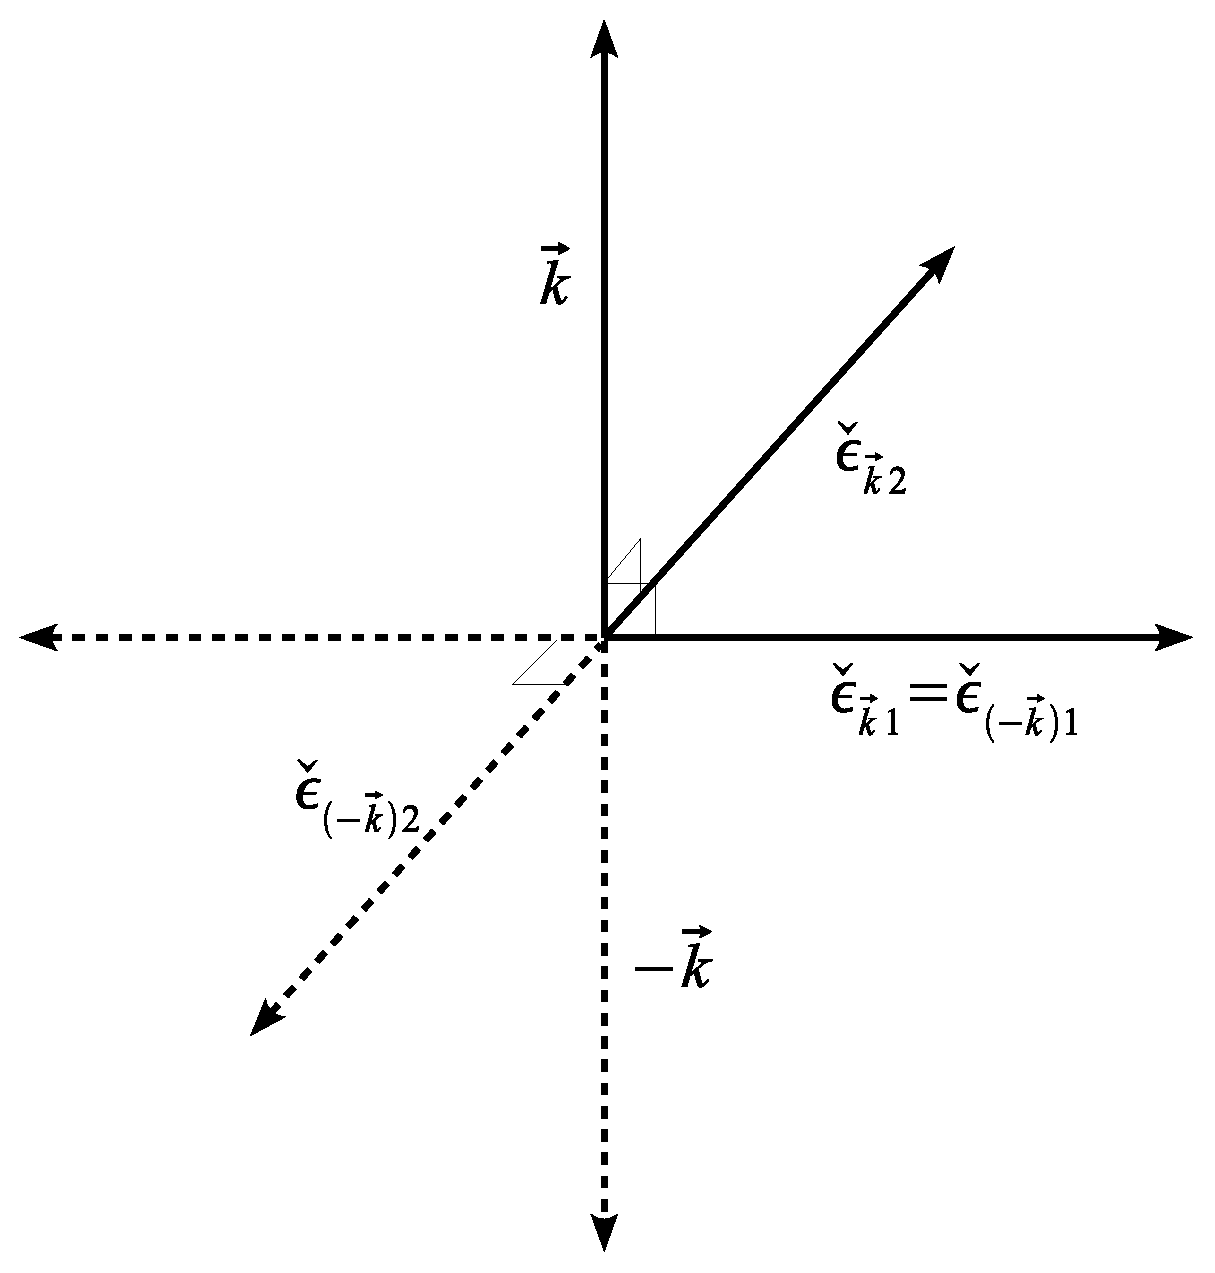
\includegraphics[height=4cm]{figs/fig-vec01.pdf}
\caption{Configuraci'on de los vectores $\check{\varepsilon}_{\vec{k}\sigma}$}
\label{figkep}
\end{center}
\end{figure}
En resumen, una soluci'on general de (\ref{ecuacion de Onda para Ai}) y
(\ref{Gauge de Coulomb}) puede escribirse como
\begin{equation}
\vec{A}(\vec{x},t)  =
\sum_{\sigma,\vec{k}}N_k\,\check{\varepsilon}_{\vec{k}\sigma}\left\{
a_{\vec{k}\sigma}(t)e^{i\vec{k}\cdot\vec{x}}+a_{\vec{k}\sigma}^*(t)e^{-i\vec{k}
\cdot\vec{x}}\right\} ,
\end{equation} 
es decir, como una superposici'on de ondas planas transversales, con dos modos
fundamentales independientes, uno para cada $\sigma$, denominadas
\textit{polarizaciones}. Es por esto que los vectores
$\check{\varepsilon}_{\vec{k}\sigma}$ son llamados \textit{vectores de
polarizaci'on}.

Como consecuencia, de (\ref{Ei(Ai)}) y (\ref{Bi(Ai)}) encontramos:
\begin{eqnarray}
\vec{E}(\vec{x},t)  & =
&\frac{i}{c}\sum_{\sigma,\vec{k}}N_k\,\check{\varepsilon}_{\vec{k}\sigma}\omega_
{k}\left\{
a_{\vec{k}\sigma}e^{i\vec{k}\cdot\vec{x}}-a_{\vec{k}\sigma}^*e^{-i\vec{k}
\cdot\vec{x}}\right\}, \\
\vec{B}(\vec{x},t) & = &i\sum_{\sigma,\vec{k}}N_k\left(
\vec{k}\times\check{\varepsilon}_{\vec{k}\sigma}\right) \left\{
a_{\vec{k}\sigma}e^{i\vec{k}\cdot\vec{x}}-a_{\vec{k}\sigma}^*e^{-i\vec{k}
\cdot\vec{x}}\right\} ,
\end{eqnarray}
de modo que tanto el campo el'ectrico como el magn'etico est'a constituido por
ondas transversales. Adem'as la energ'ia total y el momentum lineal total para
el campo electromagn'etico respectivamente son:
\begin{eqnarray}
H & = &\sum_{\sigma,\vec{k}}\frac{\omega_{k}^2}{8\pi c^2}N_k^2L^3\left(
a_{\vec{k}\sigma}^* a_{\vec{k}\sigma}+ a_{\vec{k}\sigma}
a_{\vec{k}\sigma}^*\right)  \\
\vec{P} & = &\sum_{\sigma,\vec{k}}\frac{\omega_{k}^2}{8\pi
c^2}N_k^2L^3\,\vec{k}\,a_{\vec{k}\sigma}^* a_{\vec{k}\sigma}
\end{eqnarray}


\subsection{Densidad lagrangeana, energ'ia y momentum lineal.}

Una densidad Lagrangeana que suministra las ecuaciones de Maxwell para los
$A_{i}$ es:%
\begin{equation}
{\cal L}=\frac{1}{8\pi}\left[ \frac{1}{c^{2}}\dot{A}_{i}\dot{A}_{i}-\left(
\partial_{i}A_{j}\right) \left(
\partial_{i}A_{j}\right)\right] , \label{Densidad Lagrangeana EM}
\end{equation}
donde el campo es sujeto adicionalmente a la condici'on adicional definida por
el gauge de Coulomb,
\begin{equation}
\partial_{i}A_{i}=0.
\end{equation} 
Usando la densidad lagrangeana (\ref{Densidad Lagrangeana EM}) podemos calcular:
\begin{equation}
\pi_{i}(\vec{x},t) = \frac{1}{4\pi c^{2}}\dot{A}_{i}=-\frac{1}{4\pi c}E_{i}
\label{DensidadMomentoCanonicoConjugado EM},
\end{equation}
\begin{eqnarray}
{\cal H}(\vec{x},t)& = &\frac{1}{4\pi c^{2}}\dot{A}_{i}\dot{A}_{i}-{\cal L}
\nonumber\\
& = &\frac{1}{4\pi c^{2}}\dot{A}_{i}\dot{A}_{i}-\frac{1}{8\pi c^{2}}\dot
{A}_{i}\dot{A}_{i}+\frac{1}{8\pi}\left( \partial_{i}A_{j}\right) \left(
\partial_{i}A_{j}\right) \nonumber\\
& = &\frac{1}{8\pi c^{2}}\dot{A}_{i}\dot{A}_{i}+\frac{1}{8\pi}\left(
\partial_{i}A_{j}\right) \left( \partial_{i}A_{j}\right) \nonumber\\
& = &\frac{1}{8\pi}\left\{ \frac{1}{c^{2}}\dot{A}_{i}\dot{A}_{i}+\left(
\partial_{i}A_{j}\right) \left( \partial_{i}A_{j}\right) \right\}
\label{Densidad Hamiltoniana EM}%
\end{eqnarray}
con lo que la energ'ia total es
\begin{equation}
H =\frac{1}{8\pi}\int dV \left\{ \frac{1}%
{c^{2}}\dot{A}_{i}\dot{A}_{i}+\left( \partial_{i}A_{j}\right) \left(
\partial_{i}A_{j}\right) \right\} \label{Energia del Campo EM1}%
\end{equation}
Usando la identidad
\begin{eqnarray}
B_{i}B_{i} & = &\epsilon_{ijk}\partial_{j}A_{k}\epsilon_{ilm}\partial_{l}%
A_{m}\\
& = &\left( \delta_{jl}\delta_{km}-\delta_{jm}\delta_{kl}\right) \left(
\partial_{j}A_{k}\right) \left( \partial_{l}A_{m}\right) \\
& = &\left( \partial_{j}A_{k}\right) \left( \partial_{j}A_{k}\right)
-\left( \partial_{j}A_{k}\right) \left( \partial_{k}A_{j}\right) \\
& = &\left( \partial_{j}A_{k}\right) \left( \partial_{j}A_{k}\right)
-\partial_{j}\left( A_{k}\partial_{k}A_{j}\right) +A_{k}\partial_{j}%
\partial_{k}A_{j}\\
& = &\left( \partial_{j}A_{k}\right) \left( \partial_{j}A_{k}\right)
-\partial_{j}\left( A_{k}\partial_{k}A_{j}\right)
+A_{k}\partial_{k}(\partial_{j}A_{j})\\
& = &\left( \partial_{j}A_{k}\right) \left( \partial_{j}A_{k}\right)
-\partial_{j}\left( A_{k}\partial_{k}A_{j}\right),
\end{eqnarray}
que es v'alida bajo el supuesto que el potencial vectorial satisface el gauge de
Coulomb, podemos escribir
\begin{eqnarray}
H & = &\frac{1}{8\pi}\int dV\left\{ \frac
{1}{c^{2}}\dot{A}_{i}\dot{A}_{i}+\left( \partial_{i}A_{j}\right) \left(
\partial_{i}A_{j}\right) \right\} \nonumber\\
& = &\frac{1}{8\pi}\int dV\left\{ \frac{1}{c^{2}}\dot{A}_{i}\dot{A}%
_{i}+B_{i}B_{i}+\partial_{j}\left( A_{k}\partial_{k}A_{j}\right) \right\}
\nonumber\\
& = &\frac{1}{8\pi}\int dV\left\{ \left(E^{2}+B^{2}\right) +\partial_{j}\left(
A_{k}\partial_{k}A_{j}\right) \right\} \nonumber\\
& = &\frac{1}{8\pi}\int dV\left( E^{2}+B^{2}\right) +\frac{1}{8\pi}\int
dV\partial_{j}\left( A_{k}%
\partial_{k}A_{j}\right) \nonumber\\
& = &\frac{1}{8\pi}\int_{V}dV\left( E^{2}+B^{2}\right)
+\frac{1}{8\pi}\oint_{\partial V}dS_{j}\,A_{k}\partial_{k}%
A_{j}\nonumber\\
& = &\frac{1}{8\pi}\int_{V}dV\left( E^{2}+B^{2}\right),\label{Energia del Campo
EM2}%
\end{eqnarray}
donde la integral de volumen $\oint_{\partial V}dS_{k}A_{k}\partial_{k}A_{j}$ se
anula debido a que asumimos el campo se anula suficientemente r'apido en el
infinito.

Por otro lado, para el momentum lineal total del sistema, obtenemos:
\begin{eqnarray}
p_{i}(\vec{x},t)& = &-\frac{1}{4\pi c^{2}}\dot{A}_{j}\partial_{i}A_{j}\\
& = &\frac{1}{4\pi c}\left\{ \left( \vec{E}\times\vec{B}\right) _{i}%
-\partial_{j}\left(\frac{1}{c} \dot{A}_{j}A_{i}\right) \right\}, \label{denpem}
\end{eqnarray}
ya que, en el gauge de Coulomb,
\begin{eqnarray}
\left( \vec{E}\times\vec{B}\right) _{i} & = &\epsilon_{ijk}E_{j}B_{k}\\
& = &\epsilon_{ijk}\left( -\frac{1}{c}\dot{A}_{j}\right) \left( \epsilon_{klm}%
\partial_{l}A_{m}\right) \\
& = &-\frac{1}{c}\epsilon_{ijk}\epsilon_{klm}\dot{A}_{j}\partial_{l}A_{m}\\
& = &-\frac{1}{c}\left( \delta_{il}\delta_{jm}-\delta_{im}\delta_{jl}\right)
\dot{A}%
_{j}\partial_{l}A_{m}\\
& =
&-\frac{1}{c}\dot{A}_{j}\partial_{i}A_{j}+\frac{1}{c}\dot{A}_{j}\partial_{j}A_{i
}\\
& = &-\frac{1}{c}\dot{A}_{j}\partial_{i}A_{j}+\frac{1}{c}\partial_{j}\left(
\dot{A}_{j}A_{i}\right)
-\frac{1}{c}A_{i}\partial_{j}\dot{A}_{j}\\
& = &-\frac{1}{c}\dot{A}_{j}\partial_{i}A_{j}+\frac{1}{c}\partial_{j}\left(
\dot{A}_{j}A_{i}\right)
-\frac{1}{c}A_{i}\partial_{t}\left( \partial_{j}A_{j}\right)\\
& = &-\frac{1}{c}\dot{A}_{j}\partial_{i}A_{j}+\frac{1}{c}\partial_{j}\left(
\dot{A}_{j}A_{i}\right).
\end{eqnarray}
Usando (\ref{denpem}), el momentum lineal total almacenado en el campo
electromagn'etico puede escribirse como
\begin{equation}
\vec{P}=\frac{1}{4\pi c}\int_{V}dV \vec{E}\times\vec{B} ,\label{Momentum Lineal
Total EM2}%
\end{equation} 
que corresponde al conocido vector de Pointing.


\section{Cuantizaci'on}

Dentro del gauge Coulomb y en el vac'io, donde podemos elegir $\phi=0$, lo
natural ser'ia considerar al potencial vectorial $A_i(\vec{x},t) $ como nuestra
variable de campo, de modo que su momento can'onico asociado ser'ia
\begin{equation}
\pi_i(\vec{x},t) =-\frac{1}{4\pi c}E_i(\vec{x},t).
\end{equation}
Para cuantizar el campo EM libre, debemos entonces promover estas variables de
campo a operadores que act'uan un espacio Hilbert, y luego conocer sus
relaciones de conmutaci'on.

Si consideramos a $A_i(\vec{x},t) $ como los campos independientes, entonces
esperar'iamos, de acuerdo al procedimiento de cuantizaci'on can'onico, que los
operadores de campo $\hat{A}_i(\vec{x},t)$ y $\hat{\pi}_i(\vec{x},t)$ satisfagan
las relaciones de conmutaci'on can'onicas
\begin{equation}
\left[\hat{A}_i(\vec{x}',t),\hat{\pi}_j(\vec{x},t)\right]
=i\hbar\,\delta_{ij}\,\delta(\vec{x}-\vec{x}') \hat{1}. \label{casicasi}
\end{equation}
Sin embargo, puede comprobarse r'apidamente que este conmutador es inconsistente
con el gauge de Coulomb
$\partial_i\hat{A}_{i}=\hat{0}$, ya que esta 'ultima condici'on implica
\begin{equation}
\partial_{j}'\left[ \hat{\pi}_i(\vec{x},t) ,\hat{A}_{j}(\vec{x}',t) \right] =
\left[ \hat{\pi}_i(\vec{x},t) ,\partial_{j}'\hat{A}_{j}(\vec{x}',t) \right] =0,
\end{equation}
pero, por otro lado, (\ref{casicasi}) requiere que
\begin{equation}
\partial_{j}'\left[ \hat{\pi}_i(\vec{x},t) ,\hat{A}_{j}(\vec{x}',t) \right]
=i\hbar\,\delta_{ij}\,\partial_{j}'\delta(\vec{x}-\vec{x}') \hat{1}\neq 0 .
\end{equation} 

Por lo tanto, no podemos usar las relaciones de conmutaci'on can'onicas para
cuantizar el campo electromagn'etico en el gauge de Coulomb.

Un camino para poder cuantizar el campo electromagn'etico de manera lo m'as
similar posible a la cuantizaci'on can'onica, es intentar modificar el lado
derecho de  (\ref{casicasi}) de modo que las nuevas relaciones de conmutaci'on
para los campos cu'anticos sean compatibles con el gauge de Coulomb. No es
dificil verificar\footnote{Usando $\nabla^2\frac{1}{\left| x_{k}-x'_{k}\right|
}=-4\pi\delta (\vec{x}-\vec{x}')$.}  que la modificaci'on requerida es 
\begin{equation}
\left[ \hat{A}_{i}(\vec{x},t) ,\hat{\pi}_{j}(\vec{x}',t) \right] =i\hbar\left\{
\delta_{ij}\delta (\vec{x}-\vec{x}')
+\frac{1}{4\pi}\partial_i\partial_j\frac{1}{\left| \vec{x}-\vec{x}'\right|
}\right\}
\hat{1}\label{Rel Conm Pi, A}
\end{equation}
Debido a que el nuevo t'ermino no se anula para $\vec{x}\neq\vec{x}'$, la
interpretaci'on estandar de la teor'ia cu'antica sugerir'ia que no es posible
medir simult'aneamente $\hat{A}_{i}(\vec{x},t)$ y $\hat{\pi}_{j}(\vec{x}',t)$ en
puntos distintos del espacio. Sin embargo, esto no representa necesariamente un
problema ya que $\hat{A}_{i}$ no es un observable (los observables son el campo
el'ectrico y el magn'etico). Podemos comprobar, por otra parte, que las nuevas
relaciones de conmutaci'on (\ref{casicasi}) implican relaciones de conmutaci'on
entre los campos el'ectricos y magn'eticos que no presentan este (aparente)
problema. En efecto, (\ref{casicasi}) implica
\begin{equation}
\left[\hat{B}_i(\vec{x},t),\hat{E}_j(\vec{x}',t)\right] =4\pi i\hbar
c\,\epsilon_{ijk}\partial_k\,\delta (\vec{x}-\vec{x}') \hat{1},
\end{equation} 
de modo que es posible medir simult'aneamente el campo el'ectrico y magn'etico
en puntos distintos del espacio. Sin embargo, estos campos no pueden
determinarse simult'aneamente con infinita precisi'on en el mismo punto del
espacio. Esto tiene como consecuencia que no puede existir un estado en el que
tanto $\vec{E}$ como $\vec{B}$ sean exactamente cero, lo que se manifiesta en
as'i llamadas, fluctuaciones del vac'io del campo electromagn'etico.

Finalmente, las relaciones 
\begin{eqnarray}
\left[\hat{A}_i(\vec{x},t),\hat{A}_j(\vec{x}',t)\right] &=&0,\\
\left[\hat{\pi}_i(\vec{x},t),\hat{\pi}_j(\vec{x}',t)\right] &=&0,
\end{eqnarray} 
completan las relaciones de conmutaci'on necesarias para la cuantizaci'on del
campo.



\subsection{Operadores de creaci'on y desctrucci'on}
An'alogamente al caso del campo escalar, puede mostrarse a partir de las
relaciones de conmutaci'on que los campos cu'anticos satisfacen las mismas
ecuaciones diferenciales que sus an'alogos cl'asicos.

Por lo tanto, podemos usar expansiones para los operadores de campo an'alogas a
aquellas del caso cl'asico, es decir,
\begin{eqnarray}
\hat{\vec{A}}(\vec{x},t)  &=&
\sum_{\vec{k},\sigma}N_k\,\check{\varepsilon}_{\vec{k}\sigma}\left\{
\hat{a}_{\vec{k}\sigma}(t)e^{i\vec{k}\cdot\vec{x}}+\hat{a}_{\vec{k}\sigma}
^\dagger (t)e^{-i\vec{k}\cdot\vec{x}}\right\} ,\\
\hat{\vec{E}}(\vec{x},t)  & =
&\frac{i}{c}\sum_{\vec{k},\sigma}N_k\,\check{\varepsilon}_{\vec{k}\sigma}\omega_
{k}\left\{
\hat{a}_{\vec{k}\sigma}e^{i\vec{k}\cdot\vec{x}}-\hat{a}_{\vec{k}\sigma}^\dagger
e^{-i\vec{k}\cdot\vec{x}}\right\}, \\
\hat{\vec{B}}(\vec{x},t) & = &i\sum_{\vec{k},\sigma}N_k\left(
\vec{k}\times\check{\varepsilon}_{\vec{k}\sigma}\right) \left\{
\hat{a}_{\vec{k}\sigma}e^{i\vec{k}\cdot\vec{x}}-\hat{a}_{\vec{k}\sigma}^\dagger
e^{-i\vec{k}\cdot\vec{x}}\right\} ,\\
\hat{H} & = &\sum_{\vec{k},\sigma}\frac{\omega_{k}^2}{4\pi c^2}N_k^2L^3\left(
\hat{a}_{\vec{k}\sigma}^\dagger \hat{a}_{\vec{k}\sigma}+ \hat{a}_{\vec{k}\sigma}
\hat{a}_{\vec{k}\sigma}^\dagger\right)  \\
\hat{\vec{P}} & = &\sum_{\vec{k},\sigma}\frac{\omega_{k}}{4\pi
c^2}N_k^2L^3\,\vec{k}\,\left( \hat{a}_{\vec{k}\sigma}^\dagger
\hat{a}_{\vec{k}\sigma}+ \hat{a}_{\vec{k}\sigma}
\hat{a}_{\vec{k}\sigma}^\dagger\right) .\\
\end{eqnarray}
De estas expresiones podemos obtener las relaciones inversas de los operadores
$\hat{a}$ y $\hat{a}^\dagger$ en funci'on de $\hat{A}_i$ y $\hat{\pi}_i$:
\begin{equation}
\hat{a}_{\vec{k}\sigma}=\frac{1}{2L^3N_k\omega_k}\int dV \left(\omega_{k}%
\hat{\vec{A}}+4\pi c^2 i \hat{\vec{\pi}}\right) \cdot
\check{\varepsilon}_{\vec{k}\sigma}e^{-i\vec{k}\cdot\vec{x}},
\end{equation}
y, como consecuencia,
\begin{equation}
\hat{a}^\dagger_{\vec{k}\sigma}=\frac{1}{2L^3N_k\omega_k}\int dV
\left(\omega_{k}%
\hat{\vec{A}}-4\pi c^2 i \hat{\vec{\pi}}\right) \cdot
\check{\varepsilon}_{\vec{k}\sigma}e^{i\vec{k}\cdot\vec{x}}%
\end{equation}
Con estas expresiones, podemos calcular los conmutadores de $\hat{a}$ y
$\hat{a}^\dagger$. Obtenemos:
\begin{eqnarray}
\left[ \hat{a}_{\vec{k}\sigma},\hat{a}_{\vec{k}'\sigma '}^{\dagger}\right]
&=&\frac{2\pi\hbar c^2}{L^3\omega_kN_k^2}\,\delta_{\sigma\sigma
'}\delta_{\vec{k},\vec{k}'}  , \label{aad}\\
\left[ \hat{a}_{\vec{k}\sigma},\hat{a}_{\vec{k}'\sigma '}\right] &=&0. 
\end{eqnarray}
En este momento, elegimos la constante $N_k$ de modo conveniente. Definimos
\begin{equation}
N_k=\sqrt{\frac{2\pi\hbar c^2}{L^3\omega_k}},
\end{equation} 
de modo que los operadores $\hat{a}$ y $\hat{a}^\dagger$ sean adimensionales y
satisfagan relaciones de conmutaci'on tipo operadores ``escalera" del oscilador
arm'onico.

En resumen los campos cu'anticos que describen el campo electromagn'etico en el
gauge de Coulomb son:
\begin{eqnarray}
\hat{\vec{A}}(\vec{x},t)  &=& \sqrt{\frac{2\pi\hbar
c^2}{L^3}}\sum_{\vec{k},\sigma}\frac{1}{\sqrt{\omega_k}}\check{\varepsilon}_{
\vec{k}\sigma}\left\{
\hat{a}_{\vec{k}\sigma}(t)e^{i\vec{k}\cdot\vec{x}}+\hat{a}_{\vec{k}\sigma}
^\dagger (t)e^{-i\vec{k}\cdot\vec{x}}\right\} , \label{Afi}\\
\hat{\vec{E}}(\vec{x},t)  & =
&i\sqrt{\frac{2\pi\hbar}{L^3}}\sum_{\vec{k},\sigma}\frac{1}{\sqrt{\omega_k}}
\check{\varepsilon}_{\vec{k}\sigma}\omega_{k}\left\{
\hat{a}_{\vec{k}\sigma}e^{i\vec{k}\cdot\vec{x}}-\hat{a}_{\vec{k}\sigma}^\dagger
e^{-i\vec{k}\cdot\vec{x}}\right\}, \\
\hat{\vec{B}}(\vec{x},t) & = &i\sqrt{\frac{2\pi\hbar
c^2}{L^3}}\sum_{\vec{k},\sigma}\frac{1}{\sqrt{\omega_k}}\left(
\vec{k}\times\check{\varepsilon}_{\vec{k}\sigma}\right) \left\{
\hat{a}_{\vec{k}\sigma}e^{i\vec{k}\cdot\vec{x}}-\hat{a}_{\vec{k}\sigma}^\dagger
e^{-i\vec{k}\cdot\vec{x}}\right\} ,\\
\hat{H} & = &\frac{\hbar}{2}\sum_{\vec{k},\sigma}\omega_k\left(
\hat{a}_{\vec{k}\sigma}^\dagger \hat{a}_{\vec{k}\sigma}+ \hat{a}_{\vec{k}\sigma}
\hat{a}_{\vec{k}\sigma}^\dagger\right)  \\
\hat{\vec{P}} & = &\frac{\hbar}{2}\sum_{\vec{k},\sigma}\vec{k}\,\left(
\hat{a}_{\vec{k}\sigma}^\dagger \hat{a}_{\vec{k}\sigma}+ \hat{a}_{\vec{k}\sigma}
\hat{a}_{\vec{k}\sigma}^\dagger\right) ,\\
\end{eqnarray}
y satisfacen las relaciones de conmutaci'on siguientes:
\begin{eqnarray}
\left[ \hat{a}_{\vec{k}\sigma},\hat{a}_{\vec{k}'\sigma '}^{\dagger}\right]
&=&\delta_{\sigma\sigma'}\delta_{\vec{k},\vec{k}'}  , \label{aadf}\\
\left[ \hat{a}_{\vec{k}\sigma},\hat{a}_{\vec{k}'\sigma '}\right] &=&0.
\label{aadf2}
\end{eqnarray}


\subsection{Vectores de Estado del Campo Electromagn'etico.}

Procedemos de manera an'aloga a como lo hicimos en el caso del campo escalar
(secci'on \ref{secints}). Usando las relaciones de conmutaci'on
(\ref{aadf})-(\ref{aadf2}) escribimos el operador energ'ia como
\begin{equation}
\hat{H}  = \hbar\sum_{\vec{k},\sigma}\,\omega_{k}\left\{
\hat{a}_{\vec{k,\sigma}}^{\dagger} \hat{a}_{\vec{k},\sigma} +\frac{1}{2}
\right\}.
\end{equation} 
En el caso del operador momentum, tendremos que
\begin{equation}
\hat{P}  = \hbar\sum_{\vec{k},\sigma}\, \vec{k}\left\{
\hat{a}_{\vec{k},\sigma}^{\dagger} \hat{a}_{\vec{k},\sigma} +\frac{1}{2}
\right\}=\hbar\sum_{\vec{k},\sigma}\,
\vec{k}\,\hat{a}_{\vec{k},\sigma}^{\dagger}\hat{a}_{\vec{k},\sigma}.
\end{equation} 
El ``operador n'umero", asociado a cada modo $(\vec{k},\sigma)$ con vector de
onda y polarizaci'on definidas, se define como:
\begin{equation}
\hat{N}_{\vec{k},\sigma}:=\hat{a}_{\vec{k},\sigma}^{\dagger}\hat{a}_{\vec{k},
\sigma} ,\label{defNa}
\end{equation}
de modo que los operadores Hamiltoniano y el momentum se escriben como:%
\begin{eqnarray}
\hat{H} & = &\hbar\sum_{\vec{k},\sigma}
\omega_{k}\hat{N}_{\vec{k},\sigma}+\frac{1}{2}\hbar\sum_{\vec{k},\sigma}
\omega_{k}  ,\\
\hat{P} & = &\hbar\sum_{\vec{k},\sigma} \vec{k}\,\hat{N}_{\vec{k},\sigma} .
\end{eqnarray}
Consecuentemente, encontramos que los conmutadores del operador n'umero con
$\hat{a}_{\vec{k},\sigma}$ y $\hat{a}_{\vec{k},\sigma}^{\dagger}$ son
\begin{eqnarray}
\left[ \hat{N}_{\vec{k},\sigma},\hat{a}_{\vec{k}',\sigma'}\right]
&=&-\delta_{k,k'}\delta_{\sigma,\sigma'}\,\hat{a}_{\vec{k},\sigma}, \\
\left[ \hat{N}_{\vec{k},\sigma},\hat{a}^{\dagger}_{\vec{k}',\sigma'}\right]
&=&\delta_{k,k'}\delta_{\sigma,\sigma'}\,\hat{a}^{\dagger}_{\vec{k},\sigma},
\end{eqnarray} 
de modo que
\begin{eqnarray}
\left[ \hat{H},\hat{a}_{\vec{k},\sigma}\right] &=&-\hbar\omega_k\,
\hat{a}_{\vec{k}}, \label{comha}\\
\left[ \hat{H},\hat{a}^{\dagger}_{\vec{k},\sigma}\right]
&=&\hbar\omega_k\,\hat{a}^{\dagger}_{\vec{k},\sigma},
\end{eqnarray} 
y
\begin{eqnarray}
\left[ \hat{P},\hat{a}_{\vec{k},\sigma}\right] &=&-\hbar \vec{k}\,
\hat{a}_{\vec{k},\sigma}, \\
\left[ \hat{P},\hat{a}^{\dagger}_{\vec{k},\sigma}\right] &=&\hbar \vec{k}\,
\hat{a}^{\dagger}_{\vec{k},\sigma} \label{compad}.
\end{eqnarray}
An'alogamente al caso escalar, estas propiedades implican que el espectro de
energ'ias y momenta del campo electromagn'etico cu'antico es discreto. Los
correspondientes cuantos de energ'ia y momentun son $h\omega_k$ y $\hbar
\vec{k}$, para un vector de onda $\vec{k}$ dado, respectivamente. El operador
$\hat{a}_{\vec{k},\sigma}$ (cuando se aplica a un estado dado) disminuye la
energ'ia y el momentum del estado del campo y es por esto interpretado como un
\textit{operador de destrucci'on de un cuanto de energ'ia y momentum del campo
electromagn'etico} (un ``fot'on"). An'alogamente,
$\hat{a}^{\dagger}_{\vec{k},\sigma}$ aumenta la energ'ia y el momentum del
estado del campo y es por esto interpretado como un \textit{operador de
creaci'on de un cuanto de energ'ia y momentum del campo electromagn'etico} (un
``fot'on"). 

La existencia de un estado de energ'ia m'inima, que denotaremos por
$\left|0\right>$, requiere que
\begin{equation}
\hat{a}_{\vec{k},\sigma}\left|0\right> =0, \qquad \forall\ \vec{k}, \forall \
\sigma .
\end{equation}
Este estado fundamental del campo cu'antico tiene momentum cero,
$\hat{P}\left|0\right> =0$, pero su energ'ia es infinita, con $E_0=
\frac{1}{2}\hbar\sum_{\vec{k},\sigma} \omega_{k} $.

Un estado de n'umero arbitrario puede entonces escribirse como
\begin{eqnarray}
\left| \dots,n_{\vec{k},\sigma},\dots,n_{\vec{k}',\sigma'},\dots\right>
&:=&\frac{1}{\sqrt{\cdots n_{\vec{k},\sigma}!\cdots
n_{\vec{k}',\sigma'}!\cdots}}\cdots \nonumber\\
&&\times\left( \hat{a}_{\vec{k},\sigma}^{\dagger}\right)
^{n_{\vec{k},\sigma}}\cdots\left( \hat{a}_{\vec{k}',\sigma'}^{\dagger}\right)
^{n_{\vec{k}',\sigma'}}\cdots\left| 0\right> ,
\end{eqnarray}
con $n_{\vec{k},\sigma}\in \mathbb{N}$, que interpretamos como un estado del
campo con $n_{\vec{k},\sigma}$ fotones cada una con energ'ia $\hbar\omega_{k}$
y momentum $\hbar \vec{k},$, $n_{\vec{k}',\sigma'}$ part'iculas con energ'ia y
momentum $\hbar\omega_{k'},$ $\hbar \vec{k}'$, etc, ya que
\begin{eqnarray}
\hat{H}\left| \dots,n_{\vec{k},\sigma},\dots,n_{\vec{k}',\sigma'},\dots\right>
&=& \left( E_0+n_{\vec{k},\sigma} \hbar\omega_k +n_{\vec{k}',\sigma'}
\hbar\omega_{k'}+\cdots\right) \nonumber\\
&&\times \left| \dots,n_{\vec{k},\sigma},\dots,n_{\vec{k}',\sigma'},\dots\right>
,\\
\hat{\vec{P}}\left|
\dots,n_{\vec{k},\sigma},\dots,n_{\vec{k}',\sigma'},\dots\right> &=& 
\left(n_{\vec{k},\sigma} \hbar \vec{k} +n_{\vec{k}',\sigma'} \hbar
\vec{k'}+\cdots\right) \nonumber\\
&&\times\left| \dots,n_{\vec{k},\sigma},\dots,n_{\vec{k}',\sigma'},\dots\right>
.
\end{eqnarray}

La acci'on de los operadores de creaci'on y destrucci'on sobre un estado $\left|
\dots,n_{\vec{k},\sigma},\dots\right>$ de n'umero del campo viene dada por
\begin{eqnarray}
\hat{a}_{\vec{k},\sigma}^{\dagger}\left| \dots,n_{\vec{k},\sigma},\dots\right> &
= &\sqrt{n_{\vec{k},\sigma}+1}\left| \dots,n_{\vec{k},\sigma}+1,\dots\right> ,\\
\hat{a}_{\vec{k},\sigma}\left| \dots,n_{\vec{k},\sigma},\dots\right> & =
&\sqrt{n_{\vec{k},\sigma}}\left|
\dots,n_{\vec{k},\sigma}-1,\dots\right> .
\end{eqnarray}


Estos estados forman una base ortonormal y completa del espacio de Hilbert
asociado a los operadores $\hat{N}_{\vec{k}\sigma}$ , $\hat{H}$ y
$\hat{\vec{P}},$ es decir:%
\begin{equation}
\left\langle 
\dots,n_{\vec{k}_1,\sigma_1},\dots,n_{\vec{k}_2,\sigma_2},\dots\right| \left. 
\dots,n'_{\vec{k}_1,\sigma_1},\dots,n'_{\vec{k}_2,\sigma_2},\dots\right>  =
\cdots\delta_{n_{\vec{k}_1,\sigma_1},n'_{\vec{k}_2,\sigma_2}}\delta_{n_{\vec{k}
_2,\sigma_2},n'_{\vec{k}_2,\sigma_2}}\cdots
\end{equation} 
\begin{equation}
\cdots\sum_{\vec{k}_1\sigma_1}\cdots\sum_{\vec{k}_2\sigma_2}\cdots\left|
\dots,n_{\vec{k}_1,\sigma_1},\dots,n_{\vec{k}_2,\sigma_2},\dots\right>
\left\langle
\dots,n_{\vec{k}_1,\sigma_1},\dots,n_{\vec{k}_2,\sigma_2},\dots\right|  =
\hat{1}.
\end{equation} 

Con esto, hemos completado la cuantizaci'on del campo electromagn'etico libre.
El pr'oximo paso es estudiar las consecuencias de la cuantizaci'on y, en
particular, la interacci'on del campo electromagn'etico cu'antico con la
materia.

\chapter{Interacci'on del campo electromagn'etico cuantizado con la
materia.}

\section{Interacci'on del campo electromagn'etico cl'asico con la
materia}
\subsection{Lagrangeano cl'asico}
El lagrangeano de una part'icula (no-relativista) de masa $m$ y carga $q$
movi'endose en un campo electromagn'etico, es dado por 
\begin{equation}
L=\frac{1}{2}m\dot{\vec{x}}^2+\frac{q}{c}\vec{A}\cdot \dot{\vec{x}}-q\varphi ,
\label{lagc}
\end{equation}
donde $\vec{A}=\vec{A}\left( \vec{x},t\right) $ y $\varphi =\varphi
\left( \vec{x},t\right) $ son el potencial vectorial y escalar del campo
electromagn'etico en la posici'on $\vec{x}$ y el instante $t$.

El momentum conjugado $\vec{p}$ es dado por 
\begin{equation}
\vec{p}=\frac{\partial L}{\partial
\dot{\vec{x}}}=m\dot{\vec{x}}+\frac{q}{c}\vec{A} \label{pc},
\end{equation}
y las ecuaciones de Lagrange nos dirigen a 
\begin{equation}
m \ddot{\vec{x}}=q\left( \vec{E}+\frac{1}{c}\dot{\vec{x}}\times
\vec{B}\right) .
\end{equation}

En efecto,
\begin{equation}
\frac{\partial L}{\partial x_i} =q\left( \frac{1}{c}\dot{x}_{j}\partial
_iA_{j}-\partial _i\varphi \right),
\end{equation} 
\begin{equation}
\frac{d}{dt}\frac{\partial L}{\partial \dot{x}_i}=\frac{d}{dt}\left( m\dot{%
x}_i+\frac{q}{c}A_i\right) ,
\end{equation}
de modo que las ecuaciones de Euler-Lagrange son:
\begin{eqnarray}
\frac{q}{c}\partial _iA_{j}\dot{x}_{j}-q\partial _i\varphi -\frac{d}{dt}%
\left( m\dot{x}_i+\frac{q}{c}A_i\right) &=&0 ,\\
\frac{q}{c}\partial _iA_{j}\dot{x}_{j}-q\partial _i\varphi -m\ddot{x}_i-%
\frac{q}{c}\frac{d}{dt}A_i &=&0 ,\\
\frac{q}{c}\partial _iA_{j}\dot{x}_{j}-q\partial _i\varphi -\frac{q}{c}%
\frac{d}{dt}A_i &=&m\ddot{x}_i,
\end{eqnarray}
pero $\frac{d}{dt}=\frac{\partial }{\partial t}+\dot{x}_k\partial _k$, de
modo que obtenemos
\begin{eqnarray}
\frac{q}{c}\partial _iA_{j}\dot{x}_{j}-q\partial _i\varphi -\frac{q}{c}%
\frac{\partial }{\partial t}A_i-\frac{q}{c}\dot{x}_k\partial _kA_i
&=&m\ddot{x}_i, \\
\frac{q}{c}\left( \partial _iA_{j}\dot{x}_{j}-\dot{x}_k\partial
_kA_i\right) +q\left( -\partial _i\varphi -\frac{1}{c}\frac{\partial }{%
\partial t}A_i\right) &=&m\ddot{x}_i.
\end{eqnarray}
Recordando las expresiones del campo el'ectrico y magn'etico en funci'on de los
potenciales:
\begin{eqnarray}
E_i &=&-\partial _i\varphi -\frac{1}{c}\frac{\partial A_i}{\partial t}, \\
B_i &=&\varepsilon _{ijk}\partial _{j}A_k,
\end{eqnarray}
tenemos 
\begin{eqnarray}
\frac{q}{c}\dot{x}_{j}\left( \partial _iA_{j}-\partial _{j}A_i\right)
+qE_i &=&m\ddot{x}_i, \\
\frac{q}{c}\dot{x}_{j}\left( \delta _{mi}\delta _{jn}-\delta _{mj}\delta
_{in}\right) \partial _{m}A_{n}+qE_i &=&m\ddot{x}_i ,\\
\frac{q}{c}\dot{x}_{j}\varepsilon _{kij}\varepsilon _{kmn}\partial
_{m}A_{n}+qE_i &=&m\ddot{x}_i ,\\
\frac{q}{c}\varepsilon _{kij}\dot{x}_{j}B_k+qE_i &=&m\ddot{x}_i ,\\
\frac{q}{c}\varepsilon _{ijk}\dot{x}_{j}B_k+qE_i &=&m\ddot{x}_i .
\end{eqnarray}
De modo que obtenemos finalmente
\begin{equation}
m\ddot{x}_i=q\left( E_i+\frac{1}{c}\varepsilon _{ijk}\dot{x}%
_{j}B_k\right) . 
\end{equation}


\subsection{Hamiltoniano cl'asico} 

El Hamiltoniano est'a dado por la transformada de Legendre del Lagrangiano:  
\begin{equation}
H=\vec{p}\cdot \dot{\vec{x}}-L .
\end{equation}
Usando (\ref{lagc}) y (\ref{pc}), encontramos
\begin{eqnarray}
H &=&\vec{p}\cdot \dot{\vec{x}}-\left( \frac{1}{2}m\dot{\vec{x}}%
^2+\frac{q}{c}\vec{A}\cdot \dot{\vec{x}}-q\varphi \right) \\
&=&\vec{p}\cdot \dot{\vec{x}}-\frac{1}{2}m\dot{\vec{x}}^2-\frac{q%
}{c}\vec{A}\cdot \dot{\vec{x}}+q\varphi \\
&=&\vec{p}\cdot \dot{\vec{x}}-\frac{q}{c}\vec{A}\cdot
\dot{\vec{x}}-\frac{1}{2}m\dot{\vec{x}}^2+q\varphi \\
&=&\left( \vec{p}-\frac{q}{c}\vec{A}\right) \cdot \dot{\vec{x}}-%
\frac{1}{2}m\dot{\vec{x}}^2+q\varphi \\
&=&\left( \vec{p}-\frac{q}{c}\vec{A}\right) \cdot \frac{1}{m}\left( 
\vec{p}-\frac{q}{c}\vec{A}\right) -\frac{1}{2}m\frac{1}{m^2}\left( 
\vec{p}-\frac{q}{c}\vec{A}\right)^2+q\varphi \\
&=&\frac{1}{m}\left( \vec{p}-\frac{q}{c}\vec{A}\right)^2-\frac{1}{2m%
}\left( \vec{p}-\frac{q}{c}\vec{A}\right)^2+q\varphi \\
&=&\frac{1}{2m}\left( \vec{p}-\frac{q}{c}\vec{A}\right)^2+q\varphi .
\end{eqnarray}
As'i, finalmente obtenemos
\begin{equation}
H=H_{\rm libre}+H_{\rm int},
\end{equation} 
donde $H_{\rm libre}:=\frac{1}{2m} p^2$ es el hamiltoniano de una part'icula
(no-relativista) libre, y
\begin{equation}\label{Hintnorel}
H_{\rm int} =-\frac{q}{mc}\,\vec{p}\cdot\vec{A}
+\frac{q^2}{2mc^2}\,\vec{A}^2+q\varphi ,
\end{equation} 
es el hamiltoniano de interacci'on con el campo electromagn'etico.

\subsection{Interacci'on de una part'icula no-relativista con el campo
electromagn'etico cu'antico}

Describimos las propiedades cu'anticas de una part'icula de masa $m$ y carga $q$
interactuando con el campo electromag'etico cuantizado por medio del
hamiltoniano total
\begin{eqnarray}
\hat{H}&=& \hat{H}_{\rm libre}+\hat{H}'+\hat{H}''+\hat{H}_{\hat{\varphi}}
+\hat{H}_{\rm rad} \label{hatH}\\
&=&\frac{1}{2m} \hat{\vec{p}}\,^2-\frac{q}{2mc}\,\left(
\hat{\vec{p}}\cdot\hat{\vec{A}}+\hat{\vec{A}}\cdot\hat{\vec{p}}\right)
+\frac{q^2}{2mc^2}\,\hat{\vec{A}}{\,}^2+q\hat{\varphi}+ \frac{1}{8\pi}\int dV
(\hat{E}^2+\hat{B}^2) ,
\end{eqnarray} 
donde $\hat{\vec{p}}$ es el operador momentum de la part'icula, que satisface
las usuales relaciones de conmutaci'on usadas en la mec'anica cu'antica de una
part'icula, es decir, $\left[ \vec{x}_i,\vec{p}_j\right]
=i\hbar\delta_{i,j}\hat{1}$ (en la
representaci'on coordenada $\vec{p}_j=-i\hbar \partial_j$)	, y
$(\hat{\varphi},\hat{\vec{A}})$ son los campos cu'anticos que describen el campo
electromagn'etico. Adem'as, hemos dividido los t'erminos del hamiltoniano de
interacci'on en
\begin{eqnarray}
\hat{H}'&:=&-\frac{q}{2mc}\,\left(
\hat{\vec{p}}\cdot\hat{\vec{A}}+\hat{\vec{A}}\cdot\hat{\vec{p}}\right),\\
\hat{H}''&:=&\frac{q^2}{2mc^2}\,\hat{\vec{A}}{\,}^2, \\
\hat{H}_{\hat{\varphi}}&:=&q\hat{\varphi} .
\end{eqnarray} 
En el gauge de Coulomb, s'olo $\hat{H}'$ y $\hat{H}''$ contribuyen a la
interacci'on. Adem'as,
$\hat{\vec{p}}\cdot\hat{\vec{A}}-\hat{\vec{A}}\cdot\hat{\vec{p}}=-i\hbar(\vec{
\nabla}\cdot \hat{\vec{A}}) \hat{1}=0$ (cuando act'uan sobre un vector del
espacio de Hilbert). Finalmente, el operador $\hat{\vec{A}}$ que describe el
campo electromagn'etico cuantizado (libre) tiene la forma (\ref{Afi}), de modo
que
\begin{eqnarray}
\hat{H}'&=&-\frac{e}{mc}\sqrt{\frac{2\pi\hbar
c^2}{L^3}}\sum_{\vec{k},\sigma}\frac{\hat{\vec{p}}\cdot\check{\varepsilon
}_{\vec{k}\sigma}}{\sqrt{\omega_k}}\left\{ \hat{a}_{\vec{k}\sigma}%
e^{i\vec{k}\cdot\vec{x}}+\hat{a}_{\vec{k}\sigma}^\dagger e^{-i\vec{k}%
\cdot\vec{x}}\right\} \label{H1},\\
\hat{H}''&=&\frac{e^2}{2mc^2}\left( \frac{2\pi\hbar
c^2}{L^3}\right)
\sum_{\vec{k},\sigma}\sum_{\vec{k}',\sigma'}\frac{\check{\varepsilon}_{\vec{k}
\sigma}\cdot\check{\varepsilon}_{\vec{k}'\sigma
'}}{\sqrt{\omega_k\omega_{k'}}}\left\{\hat{a}_{\vec{k}\sigma}\hat{a}_{\vec{k}
'\sigma '}e^{i\left( \vec{k}+\vec{k}'\right)
\cdot\vec{x}}+\hat{a}_{\vec{k}\sigma}\hat{a}_{\vec{k}'\sigma
'}^\dagger e^{i\left( \vec{k}-\vec{k}'\right) \cdot\vec{x}}\right. \nonumber \\
&&\left.+\hat{a}_{\vec{k}\sigma}^\dagger \hat{a}_{\vec{k}'\sigma '}e^{-i\left(
\vec{k}-\vec{k}'\right)
\cdot\vec{x}}+\hat{a}_{\vec{k}\sigma}^\dagger \hat{a}_{\vec{k}'\sigma
'}^\dagger e^{-i\left( \vec{k}+\vec{k}'\right) \cdot\vec{x}}\right\}
.\label{H2}
\end{eqnarray} 

Para la evaluaci'on de los diferentes procesos usaremos teor'ia de
perturbaciones (dependiente del tiempo), tomando como hamiltoniano ``modelo'' a
\begin{equation}
\hat{H}_0=\hat{H}_{\rm libre}+\hat{H}_{\rm rad}, \label{H0}
\end{equation} 
que ya sabemos diagonalizar. Como base del sistema part'icula + campo
consideraremos a estados de la forma $\left|\Psi\right\rangle \left|\cdots
n_{\vec{k},\sigma}\cdots\right\rangle $. Los hamiltonianos de interacci'on
$\hat{H}'$ y
$\hat{H}''$ son entonces considerados como perturbaciones.

Es ilustrativo preguntarse cu'al es el par'ametro adimensional (y peque\~no) que
usaremos para definir la serie perturbativa de un proceso dado. Para esto,
reescribiremos $\hat{H}'$ y $\hat{H}''$ en funci'on de cantidades
adimensionales:
\begin{eqnarray}
\frac{1}{mc^2}\hat{H}'&=&-\sqrt{\frac{e^2}{\hbar
c}}\sum_{\vec{k},\sigma}\sqrt{\frac{c\lambda_c^2}{2\pi  L^3\omega_k}}\left(
\frac{\hat{\vec{p}}}{mc}\right) \cdot\check{\varepsilon
}_{\vec{k}\sigma}\left\{ \hat{a}_{\vec{k}\sigma}%
e^{i\vec{k}\cdot\vec{x}}+\hat{a}_{\vec{k}\sigma}^\dagger e^{-i\vec{k}%
\cdot\vec{x}}\right\} ,\\
\frac{1}{mc^2}\hat{H}''&=&\frac{1}{2}\left( \frac{e^2}{\hbar c }\right) 
\sum_{\vec{k},\sigma}\sum_{\vec{k}',\sigma'}\left( \frac{c\lambda_c^2}{2\pi
L^3\sqrt{\omega_k\omega_{k'}}}
\right)\check{\varepsilon}_{\vec{k}\sigma}\cdot\check{\varepsilon}_{\vec{k}
'\sigma '}\left\{\hat{a}_{\vec{k}\sigma}\hat{a}_{\vec{k}'\sigma '}e^{i\left(
\vec{k}+\vec{k}'\right) \cdot\vec{x}}\right. \nonumber \\
&&\left.++\hat{a}_{\vec{k}\sigma}\hat{a}_{\vec{k}'\sigma '}^\dagger e^{i\left(
\vec{k}-\vec{k}'\right)
\cdot\vec{x}}\hat{a}_{\vec{k}\sigma}^\dagger \hat{a}_{\vec{k}'\sigma
'}e^{-i\left( \vec{k}-\vec{k}'\right)
\cdot\vec{x}}+\hat{a}_{\vec{k}\sigma}^\dagger \hat{a}_{\vec{k}'\sigma
'}^\dagger e^{-i\left( \vec{k}+\vec{k}'\right) \cdot\vec{x}}\right\}.
\end{eqnarray} 
Aqu'i hemos reemplazado $q=e$ ($e<0$ para un electr'on). Esta expresi'on
implica que, si medimos momentum en unidades de $mc$, frecuencia en unidades
de $\frac{c\lambda_c^2}{2\pi L^3}$ (donde
$\lambda_c:=\frac{h}{mc}=\frac{2\pi\hbar}{mc}$ es la longitud de Compton del
electr'on o, en general, de la part'icula) y  energ'ia en unidades de $mc^2$,
entonces la magnitud de la interacci'on es proporcional a la \textit{constante
de structura fina} $\alpha:=\frac{e^2}{\hbar c}\approx \frac{1}{137}$, con
$\hat{H}'\sim O(\sqrt{\alpha}$) y $\hat{H}''\sim O(\alpha)$. Podemos adoptar a
$\alpha$ como el par'ametro adimensional ($\ll 1$) con respecto al cual
calcularemos nuestra expansi'on perturbativa. Debido a que $\alpha\propto e^2$,
la serie perturbativa puede considerarse formalmente en potencias de la carga
$e$, con $\hat{H}'\sim O(e)$ y $\hat{H}''\sim O(e^2)$.

\subsection{Teor'ia de Perturbaciones y regla de oro de Fermi}

Regla de Oro de Fermi: La probabilidad por unidad de tiempo que ocurra la
transici'on entre el estado inicial $\left| i\right\rangle $ y el estado final
$\left|
f\right\rangle $ de un sistema cu'antico, es
\begin{equation}
\left( \frac{P}{t}\right)=\frac{2\pi}{\hbar}\left|
M_{\rm fi}\right|^2\delta\left( E_f%
-E_i\right) ,\label{Fermi Rule}%
\end{equation}
donde $M_{\rm fi}$ es la \textit{matriz de transici'on} dada por:%
\begin{equation}
M_{\rm fi}:=\left\langle f\right| \hat{H}_{int}\left| i\right\rangle 
+\sum_{I}\frac{\left\langle f\right| \hat{H}_{int}\left|
I\right\rangle  \left\langle I\right| \hat{H}_{int}\left|
i\right\rangle  }{E_i-E_{I}}+\sum_{I,II}\frac{\left\langle f\right|
\hat{H}_{int}\left| I\right\rangle  \left\langle I\right| \hat{H}%
_{int}\left| II\right\rangle  \left\langle II\right| \hat{H}%
_{int}\left| i\right\rangle  }{\left( E_i-E_{I}\right) \left(
E_i-E_{II}\right) }+\dots,\label{Mfi(1)}%
\end{equation}
con $\left| I\right\rangle  $ y $\left| II\right\rangle  $ todos los
posibles estados intermedios del sistema. 

En nuestro caso tenemos que el hamiltoniano de interacci'on es de la forma
\begin{equation}
\hat{H}_{int}=\hat{H}'+\hat{H}'' .\label{Hint}%
\end{equation}
Al reemplazar (\ref{Hint}) en (\ref{Mfi(1)}), encontramos que la matriz de
puede escribirse como:%
\begin{eqnarray}
M_{\rm fi} & = &\left\langle f\right| \left( \hat{H}'+\hat{H}''\right)
\left| i\right\rangle  +\sum_{I}\frac{\left\langle f\right| \left(
\hat{H}'+\hat{H}''\right) \left| I\right\rangle  \left\langle
I\right| \left( \hat{H}'+\hat{H}''\right) \left|i\right\rangle  }{E_i-E_{I}}\\
&& +\sum_{I,II}\frac{\left\langle f\right| \left( \hat
{H}'+\hat{H}''\right) \left| I\right\rangle  \left\langle
I\right| \left( \hat{H}'+\hat{H}''\right) \left|
II\right\rangle  \left\langle II\right| \left( \hat{H}'+\hat
{H}''\right) \left| i\right\rangle  }{\left( E_i-E_{I}\right) \left(
E_i-E_{II}\right) }+\dots\\
& = &\left\langle f\right| \hat{H}'\left| i\right\rangle 
+\left\langle f\right| \hat{H}''\left| i\right\rangle 
+\sum_{I}\frac{\left\langle f\right| \hat{H}'\left|
I\right\rangle  \left\langle I\right| \hat{H}'\left|
i\right\rangle  }{E_i-E_{I}}+\sum_{I}\frac{\left\langle f\right| \hat
{H}'\left| I\right\rangle  \left\langle I\right| \hat
{H}''\left| i\right\rangle  }{E_i-E_{I}}\\
&&+\sum_{I}\frac{\left\langle f\right| \hat{H}^{''
}\left| I\right\rangle  \left\langle I\right| \hat{H}^{'
}\left| i\right\rangle  }{E_i-E_{I}}+\sum_{I}\frac{\left\langle
f\right| \hat{H}''\left| I\right\rangle  \left\langle
I\right| \hat{H}''\left| i\right\rangle  }{E_i-E_{I}%
}+\dots
\end{eqnarray}

\section{Absorci'on de fotones por un electr'on: Contribuci'on de primer
orden en $\hat{H}'$.}

Esquem'aticamente, la absorci'on del fot'on $\vec{k}_i\sigma_i$, a primer
orden en $\hat{H}'$ corresponde al diagrama mostrado en la figura \ref{absfot}
\begin{figure}
\begin{center}
\begin{fmffile}{d1}
\begin{fmfgraph*}(50,60)
  \fmfbottom{ei,f}\fmflabel{$q_i$}{ei}\fmflabel{$k$}{f}
  \fmftop{ef}\fmflabel{$q_f$}{ef}
  \fmf{fermion}{ei,v1,ef}
  \fmf{photon}{f,v1}
 \end{fmfgraph*}
\end{fmffile}
\end{center}
\caption{Proceso de primer orden en $\hat{H}'$ para la absorci'on de un fot'on.}
\label{absfot}
\end{figure} 
En este caso, consideramos los estados iniciales y finales dados por
\begin{eqnarray}
\left| i\right\rangle  & = &\left| \vec{q}_i\right\rangle  \left|
\dots,n_{\vec{k}\sigma},\dots\right\rangle  ,\\
\left| f\right\rangle  & = &\left| \vec{q}_f\right\rangle  \left|
\dots,n_{\vec{k}\sigma}-1,\dots\right\rangle  ,
\end{eqnarray}
donde $\left| \vec{q}\right\rangle $ es un estado propio de $\hat{H}_{\rm
libre}$ de momentum definido $\hbar\vec{q}$. Tomando en cuenta las condiciones
de borde periodicas (``cuantizaci'on en la caja''), estos estados, en la
representaci'on coordenada, est'an dados por
\begin{equation}\label{OP}
\psi_{\vec{q}}\left(
\vec{x}\right) = \frac{1}{\sqrt{L^3}}e^{i\frac{\vec{p}\cdot\vec{x}}{\hbar}}=
\frac{1}{\sqrt{L^3}}e^{i\vec{q}\cdot\vec{x}},
\end{equation}
con energ'ia:%
\begin{equation}
E_{q}=\frac{\left( \hbar q\right)^2}{2m}. \label{hefree}
\end{equation}

La matriz de transici'on $M_{\rm fi}$ en este caso est'a dada, a primer orden en
$e$, por
\begin{eqnarray}
M_{\rm fi} & = &\left\langle f\right| \hat{H}'\left|
i\right\rangle  \\
& = &-\frac{e}{mc}\sqrt{\frac{2\pi\hbar c^2}{L^3}}\sum_{\vec{k}',\sigma
'}\left\langle \vec{q}_f\right| \left\langle \dots,n_{\vec{k}\sigma
}-1,\dots\right|
\frac{\hat{\vec{p}}\cdot\check{\varepsilon}_{\vec{k}'\sigma
'}}{\omega_{k'}^{1/2}}\left\{ \hat{a}_{\vec{k}'\sigma '}e^{i\vec{k}
'\cdot\vec{x}}+\hat{a}_{\vec{k}'\sigma
'}^\dagger e^{-i\vec{k}'\cdot\vec{x}}\right\} \left|
\dots,n_{\vec{k}\sigma},\dots\right\rangle 
\left| \vec{q}_i\right\rangle  \nonumber \\
& = &-\frac{e}{mc}\sqrt{\frac{2\pi\hbar c^2}{L^3}}\sum_{\vec{k}',\sigma
'}\left\{
\left\langle \dots,n_{\vec{k}\sigma}-1,\dots\right|
\hat{a}_{\vec{k}'\sigma'}\left| \dots,n_{\vec{k}\sigma},\dots\right\rangle 
\left\langle \vec{q}_f\right|
\frac{\hat{\vec{p}}\cdot\check{\varepsilon}%
_{\vec{k}'\sigma '}}{\omega_{k'}^{1/2}}e^{i\vec{k}'\cdot\vec{x}}\left|
\vec{q}_i\right\rangle  \right. \nonumber \\
&& \qquad \left.+\left\langle \dots,n_{\vec{k}\sigma}-1,\dots\right|
\hat{a}_{\vec{k}'\sigma '}^\dagger \left|
\dots,n_{\vec{k}\sigma},\dots\right\rangle 
\left\langle
\vec{q}_f\right|
\frac{\hat{\vec{p}}\cdot\check{\varepsilon}_{\vec{k}'\sigma
'}}{\omega_{k'}^{1/2}}e^{-i\vec{k}'\cdot\vec{x}}\left| \vec{q}_i\right\rangle 
\right\} \\
& = &-\frac{e}{mc}\sqrt{\frac{2\pi\hbar c^2}{L^3}}\sum_{\vec{k}',\sigma
'}\left\{\left\langle \dots,n_{\vec{k}\sigma}-1,\dots\right|
\hat{a}_{\vec{k}'\sigma '}\left|
\dots,n_{\vec{k}\sigma},\dots\right\rangle \delta_{\vec{k},\vec{k}'}\delta_{
\sigma,\sigma '}
\left\langle \vec{q}%
_f\right|\frac{\hat{\vec{p}}\cdot\check{\varepsilon}_{\vec{k}
'\sigma'}}{\omega_{k'}^{1/2}}e^{i\vec{k}'\cdot\vec{x}}\left|
\vec{q}_i\right\rangle \right\}\\
& = &-\frac{e}{mc}\sqrt{\frac{2\pi\hbar
c^2}{L^3\omega_k}}\left\{\left\langle
\dots,n_{\vec{k}\sigma}-1,\dots\right| \hat{a}_{\vec{k}\sigma}\left|
\dots,n_{\vec{k}\sigma},\dots\right\rangle  \left\langle
\vec{q}_f\right|\hat{\vec{p}}\cdot\check{\varepsilon}_{\vec{k}
\sigma}e^{i\vec{k}\cdot\vec{x}}\left|\vec{q}_i\right\rangle  \right\}\\
& = &-\frac{e}{mc}\sqrt{\frac{2\pi\hbar
c^2}{L^3\omega_k}}\left\{\sqrt{n_{\vec{k}\sigma}}\left\langle
\dots,n_{\vec{k}\sigma}-1,\dots\right|\left.
\dots,n_{\vec{k}\sigma}-1,\dots\right\rangle  \left\langle
\vec{q}_f\right|\hat{\vec{p}}\cdot\check{\varepsilon}_{\vec{k}
\sigma}e^{i\vec{k}\cdot\vec{x}}\left|\vec{q}_i\right\rangle  \right\}\\
& = &-\frac{e}{mc}\sqrt{\frac{2\pi\hbar c^2}{L^3\omega_k}}\left\langle
\vec{q}_f\right| \hat{\vec{p}}\cdot\check{\varepsilon}%
_{\vec{k}\sigma}e^{i\vec{k}\cdot\vec{x}}\left| \vec{q}_i\right\rangle 
\sqrt{n_{\vec{k}\sigma}}.
\end{eqnarray}

Por lo tanto, usando la ecuaci'on (\ref{OP}) vemos que:%
\begin{eqnarray}
\left\langle \vec{q}_f\right| \hat{\vec{p}}\cdot
\check{\varepsilon}_{\vec{k}\sigma}e^{i\vec{k}\cdot\vec{x}}\left| \vec
{q}_i\right\rangle  & \propto&\int_{V}\psi_{\vec{q}_f}^{\ast}\left(
\vec{x}\right) e^{i\vec{k}\cdot\vec{x}}\psi_{\vec{q}_i}\left( \vec
{x}\right) dV\\
& = &\int_{V}\left( \frac{1}{\sqrt{L^3}}e^{-i\vec{q}_f\cdot\vec{x}%
}\right) e^{i\vec{k}\cdot\vec{x}}\left( \frac{1}{\sqrt{L^3}}e^{i\vec
{q}_i\cdot\vec{x}}\right) dV\\
& = &\frac{1}{L^3}\int_{L^3}e^{-i\left\{ \vec{q}_f-\left( \vec{q}%
_i+\vec{k}\right) \right\} \cdot\vec{x}}dV\\
& = &\frac{1}{L^3}\left\{ L^3\delta_{\vec{q}_f,\vec{q}_i+\vec{k}%
}\right\} \\
& = &\delta_{\vec{q}_f,\vec{q}_i+\vec{k}} \, ,
\end{eqnarray}
que expresa la conservaci'on del momentum:
\begin{equation}
\hbar\vec{q}_f=\hbar\vec{q}_i+\hbar\vec{k} \, ,\label{Conservacion Momentum}
\end{equation}
mientras que de (\ref{hefree}) y de la delta en (\ref{Fermi Rule}), obtenemos la
condici'on de conservaci'on de la energ'ia:
\begin{eqnarray}
E_f & = &E_i\, ,\\
E_0+\frac{\left( \hbar\vec{q}_f\right)^2}{2m}+\hbar\omega_k\left(
n_{\vec{k}\sigma}-1\right) & = &E_0+\hbar\omega_kn_{\vec{k}\sigma}%
+\frac{\left( \hbar\vec{q}_i\right)^2}{2m} \, ,\\
% \frac{\left( \hbar\vec{q}_f\right)^2}{2m}+\hbar\omega_kn_{\vec
% {k}\sigma}-\hbar\omega_k & = &\hbar\omega_kn_{\vec{k}\sigma}+\frac{\left(
% \hbar\vec{q}_i\right)^2}{2m} \, ,\\
\frac{\left( \hbar\vec{q}_f\right)^2}{2m} & = &\hbar\omega_k%
+\frac{\left( \hbar\vec{q}_i\right)^2}{2m}.\label{Conservacion Energia}%
\end{eqnarray}

Sin embargo, es f'acil mostrar que (\ref{Conservacion Energia}) y
(\ref{Conservacion Momentum}) no pueden ser satisfechas simult'aneamente. Por lo
tanto, es imposible que un electr'on libre (aislado) absorba un fot'on. Este
resultado es v'alido tambi'en para ordenes superiores en la teor'ia de
perturbaciones.


\section{Scattering entre fotones y electrones libres.}

Consideraremos procesos de scattering del tipo mostrado en la figura
\ref{scatef}.
\begin{figure}
\begin{center}
\begin{fmffile}{d2}
\begin{fmfgraph*}(50,70)
  \fmfbottom{e1,f1}\fmflabel{$q_i$}{e1}\fmflabel{$k_i$}{f1}
  \fmftop{e2,f2}\fmflabel{$q_f$}{e2}\fmflabel{$k_f$}{f2}
  \fmfblob{0.5w}{v1}
  \fmf{fermion}{e1,v1,e2}
  \fmf{photon}{f1,v1,f2}
 \end{fmfgraph*}
\end{fmffile}
\end{center}
\caption{Scattering de fotones con electrones libres. Inicialmente un
electr'on en el estado $\left| \vec{q}_i\right\rangle  $ absorve un
fot'on $\vec{k}_i\sigma_i.$ El resultado del proceso es un fot'on
emitido $\vec{k}_f\sigma_f$ y el electr'on en el estado $\left|
\vec{q}_f\right\rangle  .$}
\label{scatef}
\end{figure} 
En este caso, consideraremos que los estados inicial y final est'an dados por
\begin{eqnarray}
\left| i\right\rangle  & = &\left| \vec{q}_i\right\rangle  \left|
\dots,n_{\vec{k}_i\sigma_i},\dots,n_{\vec{k}_f\sigma_f},\dots\right\rangle 
=\left| \vec{q}_i\right\rangle  \left| \gamma_i\right\rangle 
,\label{|i>} \\
\left| f\right\rangle  & = &\left| \vec{q}_f\right\rangle  \left|
\dots,n_{\vec{k}_i\sigma_i}-1,\dots,n_{\vec{k}_f\sigma_f}%
+1,\dots\right\rangle  =\left| \vec{q}_f\right\rangle  \left|
\gamma_f\right\rangle  .\label{|f>} 
\end{eqnarray}
En la pr'actica es conveniente describir un proceso de scattering por medio
de la correspondiente \textit{secci'on diferencial de scattering}
\begin{equation}
\frac{d\sigma}{d\Omega}:=\frac{\left( \text{N'umero de part'iculas
emitidas por unidad de tiempo y de 'angulo s'olido}\right) }{\left(
\text{N'umero de part'iculas incidentes por unidad de 'area y de
tiempo}\right)} .
\end{equation}
En el contexto de la teor'ia cu'antica, la secci'on diferencial puede
calcularse dividiendo la probabilidad por unidad de tiempo de que la part'icula
final (en nuestro caso, el fot'on final) sea emitido en el 'angulo s'olido
$d\Omega$ en la direcci'on determinada por los 'angulos de scattering
$(\vartheta,\phi)$, por la densidad de flujo de probabilidad del haz incidente:
\begin{equation}
\frac{d\sigma}{d\Omega}
d\Omega=\frac{(P/t)(\vartheta,\phi,d\Omega)}{j_0},
\end{equation}
 Note que $\frac{d\sigma}{d\Omega}$ tiene unidades de 'area. 
La densidad de flujo de probabilidad de fotones incidentes est'a dada por:
\begin{equation}
j_{0,\rm fotones}=\frac{n_{\vec{k}_i\sigma_i}}{L^3}c,
\end{equation}

De modo que
\begin{eqnarray}
d\sigma_{\vec{k},\sigma} &=&
\frac{\left(\frac{P}{t}\right)_{\text{Scattering}}}
{\frac{n_{\vec{k} _i\sigma_i}} {L^3}c}\nonumber\\
& = &\frac{2\pi L^3}{\hbar cn_{\vec{k}_i\sigma_i}}\left|
M_{\rm fi}\right|^2\delta\left( E_f-E_i\right).
\label{Seccion Transversal Absorcion}%
\end{eqnarray}
Para evaluar la matriz de transici'on, s'olo nos interesan los t'erminos que
produzcan
procesos del tipo mostrado en la figura \ref{scatef}. Estos t'erminos est'an
presentes a primer orden en $\hat{H}
''$, mientras que $\hat{H}'$ s'olo puede contribuir con t'erminos de
segundo orden en la serie perturbativa. En consecuencia, a orden $e^2$, la
matriz $M_{\rm fi}$ se reduce a:
\begin{equation}
M_{\rm fi}=\left\langle f\right| \hat{H}''\left|
i\right\rangle  +\sum_{I}\frac{\left\langle f\right| \hat{H}^{'
}\left| I\right\rangle  \left\langle I\right| \hat{H}^{'
}\left| i\right\rangle  }{E_i-E_{I}}.\label{Mfi(3)}%
\end{equation}

\subsection{Contribuci'on de primer orden en $\hat{H}''$}

El hamiltoniano $\hat{H}''$ es funci'on de combinaciones del tipo $
\hat{a}_{\vec{k}\sigma}\hat{a}_{\vec{k}'\sigma '}$,
$\hat{a}_{\vec{k}\sigma}\hat{a}_{\vec{k}'\sigma'}^\dagger $, 
$\hat{a}_{\vec{k}\sigma}^\dagger \hat{a}_{\vec{k}'\sigma'}$, 
$\hat{a}_{\vec{k}\sigma}^\dagger \hat{a}_{\vec{k}'\sigma '}^\dagger $, de los
operadores de creaci'on y destrucci'on, los cuales describen procesos de
absorci'on-absorci'on, emisi'on-absorci'on, absorci'on-emisi'on y
emisi'on-emisi'on, respectivamente. De 'estos, s'olo los t'erminos del tipo
absorci'on-emisi'on (emisi'on-absorci'on), representados por diagramas como el
de la figura
\ref{scfefe}, contribuyen al proceso de scattering aqu'i considerado.
\begin{figure}
\begin{center}
\begin{fmffile}{d3}
\begin{fmfchar*}(40,70)
 \fmfbottom{ei,fi}\fmflabel{$q_i$}{ei}\fmflabel{$k_i$}{fi}
 \fmftop{ef,ff}\fmflabel{$q_f$}{ef}\fmflabel{$k_f$}{ff}
 \fmf{fermion}{ei,v1,ef}
 \fmf{photon}{fi,v1}
 \fmf{photon}{v1,ff}
 %\fmfdot{v1}
 \end{fmfchar*}
\end{fmffile}
\caption{Diagrama del t'ermino de primer orden en $\hat{H}''$.}
\label{scfefe}
\end{center}
\end{figure}

De este modo, tenemos que:
\begin{eqnarray}
\left\langle f\right| \hat{H}''\left| i\right\rangle  &=&\left(
\frac{e^2}{2mc^2}\right) \left( \frac{2\pi\hbar c^2}{L^3}\right)
\sum_{\vec{k},\sigma,\vec{k}',\sigma '}\left\langle \vec{q}_f\right|
\left\langle
\dots,(n_{\vec{k}_i\sigma_i}-1),\dots,n_{\vec{k}_f\sigma_f}+1,
\dots\right| \frac{\check
{\varepsilon}_{\vec{k}\sigma}\cdot\check{\varepsilon}_{\vec{k}'\sigma'}}{\sqrt{
\omega_k\omega_{k'}}} \nonumber\\
&& \times\left\{ \hat{a}_{\vec{k}\sigma}\hat{a}_{\vec{k}'\sigma
'}^\dagger e^{i\left(
\vec{k}-\vec{k}'\right)\cdot\vec{x}}+\hat{a}_{\vec{k}\sigma}^\dagger \hat{a}_{
\vec{k}'\sigma'}e^{-i\left(\vec{k}-\vec{k}'\right)\cdot\vec{x}}\right\}
\left|\dots,n_{\vec{k}_i\sigma_i},\dots,n_{\vec{k}_f\sigma_f},
\dots\right\rangle  \left| \vec{q}_i\right\rangle  \\
& = &\left( \frac{e^2}{2mc^2}\right) \left( \frac{2\pi\hbar
c^2}{L^3}\right)\sum_{\vec{k},\sigma,\vec{k}',\sigma'}\frac{\check{
\varepsilon}_{\vec{k}\sigma}\cdot\check{\varepsilon}_{\vec{k}'\sigma
'}}{\sqrt{\omega_k\omega_{k'}}}\left\{\left\langle \gamma_f\right|
\hat{a}_{\vec{k}\sigma}\hat{a}_{\vec{k}'\sigma '}^\dagger \left|
\gamma_i\right\rangle  \left\langle \vec{q}_f\right| e^{i\left(
\vec{k}-\vec{k}'\right) \cdot\vec{x}}\left| \vec{q}_i\right\rangle  
\right.\nonumber\\
&&+\left\langle\left.  \gamma_f\right|
\hat{a}_{\vec{k}\sigma}^\dagger \hat{a}_{\vec{k}'\sigma '}\left|
\gamma_i\right\rangle  \left\langle \vec{q}_f\right| e^{-i\left(
\vec{k}-\vec{k}'\right) \cdot\vec{x}}\left| \vec{q}_i\right\rangle \right\}\\
& = &\left( \frac{e^2}{2mc^2}\right) \left( \frac{2\pi\hbar c^2}{L^3}\right)
\sum_{\vec{k},\sigma,\vec{k}',\sigma'}\frac{\check{\varepsilon}_{\vec{k}\sigma}
\cdot\check{\varepsilon}_{\vec{k}'\sigma
'}}{\sqrt{\omega_k\omega_{k'}}}\left\{\left\langle \gamma_f\right|
\hat{a}_{\vec{k}\sigma}\hat{a}_{\vec{k}'\sigma '}^\dagger \left|
\gamma_i\right\rangle 
\delta_{\vec{k},\vec{k}_i}\delta_{\vec{k}',\vec{k}_f}\delta_{\sigma,\sigma_i}
\delta_{\sigma ',\sigma_f}\left\langle \vec{q}_f\right| e^{i\left(
\vec{k}-\vec{k}'\right) \cdot\vec{x}}\left| \vec{q}_i\right\rangle  \right.
\nonumber\\
% &&\left. +\left\langle \gamma_f\right|
% \hat{a}_{\vec{k}\sigma}\hat{a}_{\vec{k}'\sigma '}^\dagger \left|
% \gamma_i\right\rangle 
% \delta_{\vec{k},\vec{k}_f}\delta_{\vec{k}',\vec{k}_i}\delta_{\sigma,\sigma_{
% f}}\delta_{\sigma ',\sigma_i}\left\langle \vec{q}_f\right| e^{i\left(
% \vec{k}-\vec{k}'\right) \cdot\vec{x}}\left| \vec{q}_i\right\rangle  \right.
% \nonumber\\
% && +\left\langle \gamma_f\right| \hat{a}_{\vec{k}\sigma}^\dagger \hat
% {a}_{\vec{k}'\sigma '}\left| \gamma_i\right\rangle 
% \delta_{\vec{k},\vec{k}_i}\delta
% _{\vec{k}',\vec{k}_f}\delta_{\sigma,\sigma_i}\delta_{\sigma
% ',\sigma_f}\left\langle \vec{q}_f\right| e^{-i\left( \vec{k}-\vec{k}'\right)
% \cdot\vec{x}}\left| \vec{q}_i\right\rangle  \nonumber\\
&&\left.+\left\langle \gamma_f\right|
\hat{a}_{\vec{k}\sigma}^\dagger \hat{a}_{\vec{k}'\sigma '}\left|
\gamma_i\right\rangle 
\delta_{\vec{k},\vec{k}_f}\delta_{\vec{k}',\vec{k}_i}\delta_{\sigma,\sigma_{
f}}\delta_{\sigma ',\sigma_i}\left\langle \vec{q}_f\right| e^{-i\left(
\vec{k}-\vec{k}'\right) \cdot\vec{x}}\left| \vec{q}_i\right\rangle \right\}
\nonumber\\
& = &\left( \frac{e^2}{2mc^2}\right) \left( \frac{2\pi\hbar c^2}%
{L^3}\right) \frac{\check{\varepsilon}_{\vec{k}_i\sigma_i}\cdot
\check{\varepsilon}_{_{\vec{k}_f\sigma_f}}}{\sqrt{\omega_k\omega_{k'}}}
\left\{\left\langle \gamma_f\right| \hat{a}_{\vec{k}_i\sigma_i}
\hat{a}_{_{\vec{k}_f\sigma_f}}^\dagger \left| \gamma_i\right\rangle \left\langle
\vec{q}_f\right| e^{i\left(
\vec{k}_i-\vec{k}_f\right) \cdot\vec{x}}\left| \vec{q}_i\right\rangle \right\}
\nonumber\\
&&\left.+\left\langle\gamma_f\right|\hat{a}_{_{\vec{k}_f\sigma_f}}^\dagger
\hat{a}_{_{\vec{k}_{i}\sigma_i}}\left| i_\gamma\right\rangle 
\left\langle \vec{q}_f\right| e^{-i\left(
\vec{k}_i-\vec{k}_f\right) \cdot\vec{x}}\left| \vec{q}_i%
\right\rangle \right\} \nonumber\\
& = &2\left( \frac{e^2}{2mc^2}\right) \left( \frac{2\pi\hbar c^2%
}{L^3}\right) \frac{\check{\varepsilon}_{\vec{k}_i\sigma_i}\cdot
\check{\varepsilon}_{_{\vec{k}_f\sigma_f}}}{\sqrt{\omega_{k_i}%
\omega_{k_f}}}\left\langle \vec{q}_f\right| e^{i\left( \vec{k}%
_i-\vec{k}_f\right) \cdot\vec{x}}\left| \vec{q}_i\right\rangle 
\sqrt{n_{\vec{k}_i\sigma_i}\left( n_{\vec{k}_f\sigma_f}+1\right)
}.\label{<qf|H2|qi>}
\end{eqnarray}
Usando (\ref{OP}), vemos que:%
\begin{eqnarray}
\left\langle \vec{q}_f\right| e^{i\left( \vec{k}_i-\vec{k}%
_f\right) \cdot\vec{x}}\left| \vec{q}_i\right\rangle  & = &\int
_{L^3}\left( \frac{1}{\sqrt{L^3}}e^{-i\vec{q}_f\cdot\vec{x}}\right)
e^{i\left( \vec{k}_i-\vec{k}_f\right) \cdot\vec{x}}\left( \frac
{1}{\sqrt{L^3}}e^{i\vec{q}_i\cdot\vec{x}}\right) d^3x\nonumber\\
& = &\frac{1}{L^3}\int_{L^3}e^{i\left\{ \vec{q}_i+\vec{k}_i-\left(
\vec{q}_f+\vec{k}_f\right) \right\} \cdot\vec{x}}d^3x\nonumber\\
& = &\frac{1}{L^3}\left\{ L^3\delta_{\vec{q}_f+\vec{k}_f,\vec{q}%
_i+\vec{k}_i}\right\} \nonumber\\
& = &\delta_{\vec{q}_f+\vec{k}_f,\vec{q}_i+\vec{k}_i},\label{<qf|2|qi>}%
\end{eqnarray}
que nuevamente expresa la conservaci'on del momentum en el proceso:
\begin{equation}
\hbar\left( \vec{q}_f+\vec{k}_f\right) =\hbar\left( \vec{q}_i+\vec
{k}_i\right) .\label{Conservacion Momentum 2}%
\end{equation}

La condici'on de conservaci'on de la energ'ia impuesta por la delta de Dirac
en (\ref{Fermi Rule}) implica que la probabilidad de transici'on y por tanto la
secci'on diferencial es no nula s'olo si:
\begin{eqnarray}
E_f & = &E_i,\\
E_0+\frac{\left( \hbar\vec{q}_f\right)^2}{2m}+\hbar\omega_{k_i}(n_{\vec
{k}_i\sigma_i}-1)+\hbar\omega_{k_f}(n_{\vec{k}_f\sigma_f}+1) & =
&E_0+\frac{\left( \hbar\vec{q}_i\right)
^2}{2m}+\hbar\omega_{k_i}n_{\vec{k}_i\sigma_i}+\hbar\omega_{k_f%
}n_{\vec{k}_f\sigma_f} ,\\
\frac{\left( \hbar\vec{q}_f\right)^2}{2m}+\hbar\omega_{k_f} &
=&\frac{\left( \hbar\vec{q}_i\right)
^2}{2m}+\hbar\omega_{k_i}.\label{Conservacion Energia 2}
\end{eqnarray}


As'i, reemplazando (\ref{<qf|2|qi>}) en (\ref{<qf|H2|qi>}), obtenemos:%
\begin{equation}
\left\langle f\right| \hat{H}''\left| i\right\rangle 
=2\left( \frac{e^2}{2mc^2}\right) \left( \frac{2\pi\hbar c^2}{L^3%
}\right) \frac{\check{\varepsilon}_{\vec{k}_i\sigma_i}\cdot
\check{\varepsilon}_{_{\vec{k}_f\sigma_f}}}{\sqrt{\omega_k\omega_{k'}}}
\sqrt{n_{\vec{k}_i\sigma_i}\left( n_{\vec{k}_f\sigma_f}+1\right)
}\delta_{\vec{q}_f+\vec{k}_f,\vec{q}_i+\vec{k}_i}.\label{<f|H2|i>} %
\end{equation}
Usando este resultado, (\ref{Mfi(3)}) implica que
\begin{eqnarray}
\left| M_{\rm fi}^{\left( 1\right) }\right|^2 & = &\left|
\left\langle f\right| \hat{H}''\left| i\right\rangle 
\right|^2\\
& = &\left| 2\left( \frac{e^2}{2mc^2}\right) \left( \frac{2\pi\hbar
c^2}{L^3}\right) \frac{\check{\varepsilon}_{\vec{k}_i\sigma_i}%
\cdot\check{\varepsilon}_{_{\vec{k}_f\sigma_f}}}{\sqrt{\omega_k\omega_{k'}
}}\left\langle \vec{q}_f\right| e^{i\left( \vec{k}_i-\vec{k}%
_f\right) \cdot\vec{x}}\left| \vec{q}_i\right\rangle  \sqrt{n_{\vec
{k}_i\sigma_i}\left( n_{\vec{k}_f\sigma_f}+1\right) }\right|
^2\\
& = &4\left( \frac{e^2}{2mc^2}\right)^2\left( \frac{2\pi\hbar c^2%
}{L^3}\right)^2\frac{n_{\vec{k}_i\sigma_i}\left( n_{\vec{k}%
_f\sigma_f}+1\right) \left| \check{\varepsilon}_{\vec{k}_i%
\sigma_i}\cdot\check{\varepsilon}_{_{\vec{k}_f\sigma_f}}\right|
^2}{\omega_{k_i}\omega_{k_f}}\delta_{\vec{q}_f+\vec{k}_f,\vec{q}%
_i+\vec{k}_i}.
\end{eqnarray}


Finalmente, (\ref{Fermi Rule}) se reduce a:
\begin{eqnarray}
\left( \frac{P}{t}\right)_{\text{Scattering}}&=&\frac{8\pi}{\hbar}\left(
\frac{e^2}{2mc^2}\right)^2\left(
\frac{2\pi\hbar c^2}{L^3}\right)^2\frac{\left| \check{\varepsilon
}_{\vec{k}_i\sigma_i}\cdot\check{\varepsilon}_{_{\vec{k}_f\sigma_f}%
}\right|^2}{\omega_{k_i}\omega_{k_f}}n_{\vec{k}_i\sigma_i%
}\left( n_{\vec{k}_f\sigma_f}+1\right) \nonumber\\
&& \times \delta_{\vec{q}_f+\vec{k}%
_f,\vec{q}_i+\vec{k}_i}\,\delta\left( \frac{\left( \hbar\vec{q}%
_f\right)^2}{2m}+\hbar\omega_{k_f}-\frac{\left( \hbar\vec{q}%
_i\right)^2}{2m}-\hbar\omega_{k_i}\right) .
\end{eqnarray}
El t'ermino $\left( n_{\vec{k}_f\sigma_f}+1\right) $ en la
expresi'on anterior es interpretado como \textit{emissi'on estimulada} por los
fotones $(\vec{k}_f\sigma_f)$ en el estado final. Por lo tanto, el
scattering es aumentado si esos fotones en el estado final ya est'an presentes.
A menudo este no es el caso, de modo que consideraremos
$n_{\vec{k}_f\sigma_f}=0$. En este subcaso obtenemos que la secci'on
diferencial de scattering es:%
\begin{eqnarray}
\sigma\left( \vec{k}\sigma\right) &=&\frac{8\pi L^3}{\hbar c}\left(
\frac{e^2}{2mc^2}\right)^2\left( \frac{2\pi\hbar c^2}{L^3%
}\right)^2\frac{\left| \check{\varepsilon}_{\vec{k}_i\sigma_i%
}\cdot\check{\varepsilon}_{_{\vec{k}_f\sigma_f}}\right|^2}%
{\omega_{k_i}\omega_{k_f}} \nonumber\\
&& \times \delta_{\vec{q}_f+\vec{k}_f,\vec{q}_i%
+\vec{k}_i}\delta\left( \frac{\left( \hbar\vec{q}_f\right)^2}%
{2m}+\hbar\omega_{k_f}-\frac{\left( \hbar\vec{q}_i\right)^2}%
{2m}-\hbar\omega_{k_i}\right)
.\label{Seccion Transversal Absorcion <f|H2|i> }%
\end{eqnarray}


La \textit{secci'on total de scattering} se encuentra sumando sobre todos
los estados finales del electr'on y del fot'on. Por lo tanto:%
\begin{eqnarray}
\sigma_{T} & = &\frac{8\pi L^3}{\hbar c}\left( \frac{e^2}{2mc^2%
}\right)^2\left( \frac{2\pi\hbar c^2}{L^3}\right)^2\sum_{\vec
{k}_f,\sigma_f}\sum_{\vec{q}_f}\frac{\left| \check{\varepsilon
}_{\vec{k}_i\sigma_i}\cdot\check{\varepsilon}_{_{\vec{k}_f\sigma_f}%
}\right|^2}{c^2k_ik_f} \nonumber\\
&& \times \delta_{\vec{q}_f+\vec{k}_f,\vec{q}%
_i+\vec{k}_i}\delta\left( \frac{\left( \hbar\vec{q}_f\right)^2%
}{2m}+\hbar\omega_{k_f}-\frac{\left( \hbar\vec{q}_i\right)^2}%
{2m}-\hbar\omega_{k_i}\right) \\
& = &\frac{8\pi L^3}{\hbar c^3}\left( \frac{e^2}{2mc^2}\right)
^2\left( \frac{2\pi\hbar c^2}{L^3}\right)^2\sum_{\vec{k}_f%
,\sigma_f}\frac{\left| \check{\varepsilon}_{\vec{k}_i\sigma_i}%
\cdot\check{\varepsilon}_{_{\vec{k}_f\sigma_f}}\right|^2}%
{k_ik_f} \nonumber\\
&&\times \delta\left( \frac{\hbar^2\left( \vec{q}_i+\vec{k}_i%
-\vec{k}_f\right)^2}{2m}+\hbar\omega_{k_f}-\frac{\left( \hbar\vec
{q}_i\right)^2}{2m}-\hbar\omega_{k_i}\right) ,
\end{eqnarray}
donde hemos considerado que $\omega_k=ck.$ Pasando al continuo en
coordenadas esf'ericas ($\sum_{\vec{k}_f}\rightarrow\frac{L^3}{\left(
2\pi\right) ^3}\int d^3k_f=\frac{L^3}{\left( 2\pi\right) ^3}\int
k_f^2dk_fd\Omega_f$), obtenemos
\begin{eqnarray}
\sigma_{T}&=&\hbar c\left( \frac{e^2}{mc^2}\right)
^2\sum_{\sigma_f}\int\frac{k_f}{k_i}\left|\check{\varepsilon}_{\vec{k}_{
i}\sigma_i}\cdot\check{\varepsilon}_{_{\vec{k}_f\sigma_f}}\right|^2
\nonumber\\
&&\times\delta\left( \frac{\hbar^2\left(
\vec{q}_i+\vec{k}_i-\vec{k}_f\right)^2}{2m}+c\hbar\left(
k_f-k_i\right) -\frac{\left(\hbar\vec{q}_i\right)^2}{2m}\right)
dk_fd\Omega_f,
\end{eqnarray}
y considerando la aproximaci'on $\vec{k}_i-\vec{k}_f\approx0$, tenemos que:%
\begin{eqnarray}
\sigma_{T} & = &\hbar c\left( \frac{e^2}{mc^2}\right)^2\sum
_{\sigma_f}\int\frac{k_f}{k_i}\left| \check{\varepsilon}_{\vec
{k}_i\sigma_i}\cdot\check{\varepsilon}_{_{\vec{k}_f\sigma_f}%
}\right|^2\delta\left( c\hbar\left( k_f-k_i\right) \right)
dk_fd\Omega_f\\
& = &\hbar c\left( \frac{e^2}{mc^2}\right)^2\sum_{\sigma_f}\int
\frac{k_f}{k_i}\left| \check{\varepsilon}_{\vec{k}_i\sigma_i}%
\cdot\check{\varepsilon}_{_{\vec{k}_f\sigma_f}}\right|^2\frac
{1}{c\hbar}\delta\left( k_f-k_i\right) dk_fd\Omega_f\\
& = &\left( \frac{e^2}{mc^2}\right)^2\sum_{\sigma_f}\int\frac{k_f%
}{k_i}\left| \check{\varepsilon}_{\vec{k}_i\sigma_i}\cdot
\check{\varepsilon}_{_{\vec{k}_f\sigma_f}}\right|^2\delta\left(
k_f-k_i\right) dk_fd\Omega_f\\
& = &\left( \frac{e^2}{mc^2}\right)^2\int_{\Omega_f}\sum_{\sigma
_f}\left| \check{\varepsilon}_{\vec{k}_i\sigma_i}\cdot
\check{\varepsilon}_{_{\vec{k}_f\sigma_f}}\right|^2d\Omega_f.
\end{eqnarray}
\textit{Suponiendo} que los fotones incidentes no tienen una polarizaci'on
(resultante) privilegiada, debemos \textit{promediar} sobre las dos
polarizaciones iniciales. Adem'as, sumaremos sobre las polarizaciones finales. 
*** explicar + detalladamente ***

As'i, considerando la siguiente configuraci'on geom'etrica, ver figura
\ref{geomscat}, encontramos que:
\begin{figure}[ht]
\begin{center}
	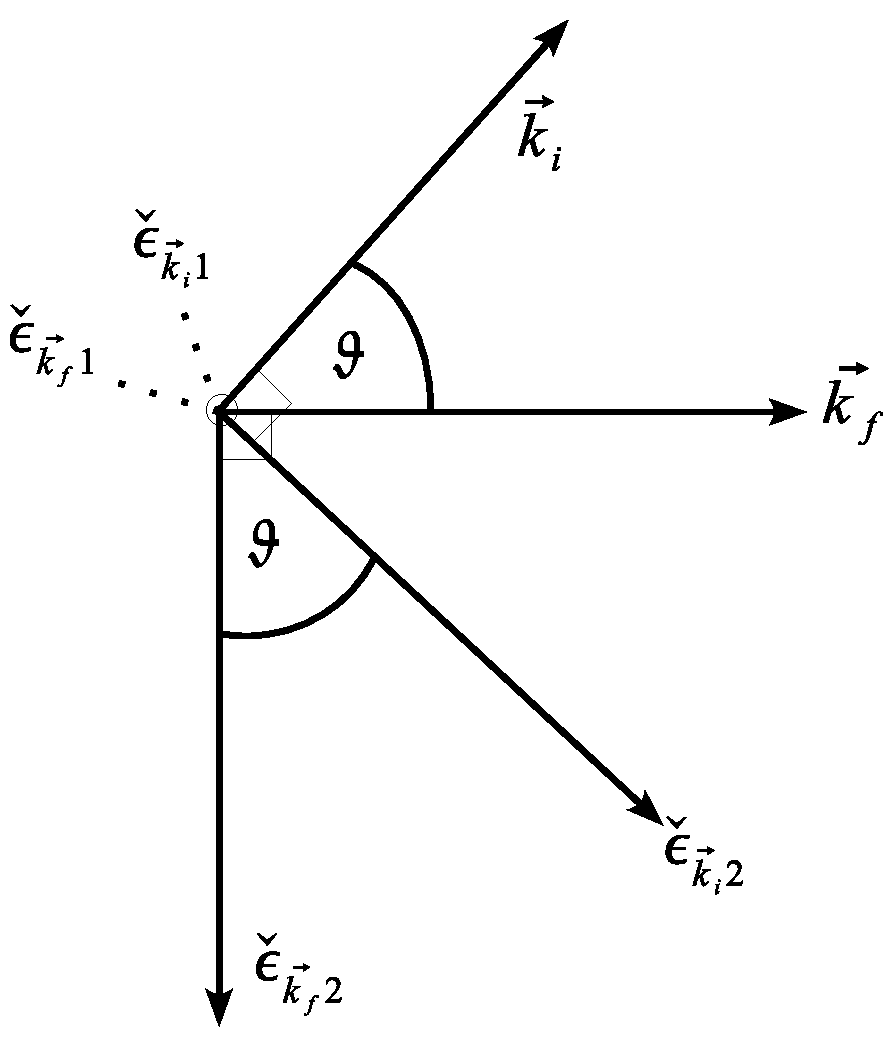
\includegraphics[height=4cm]{figs/fig-kikf.pdf}
	\caption{Geometr'ia del scattering.}
   \label{geomscat}
\end{center}
\end{figure}
\begin{eqnarray}
\frac{1}{2}\sum_{\sigma_f=1}^2\sum_{\sigma_i=1}^2\left|
\check{\varepsilon}_{\vec{k}_i\sigma_i}\cdot\check{\varepsilon}_{_{\vec
{k}_f\sigma_f}}\right|^2 & = &\frac{1}{2}\sum_{\sigma_f=1}%
^2\left\{ \left| \check{\varepsilon}_{\vec{k}_i1}\cdot\check
{\varepsilon}_{_{\vec{k}_f\sigma_f}}\right|^2+\left|
\check{\varepsilon}_{\vec{k}_i2}\cdot\check{\varepsilon}_{_{\vec{k}%
_f\sigma_f}}\right|^2\right\} \\
& = &\frac{1}{2}\left\{ \left| \check{\varepsilon}_{\vec{k}_i1}%
\cdot\check{\varepsilon}_{_{\vec{k}_f1}}\right|^2+\left|
\check{\varepsilon}_{\vec{k}_i2}\cdot\check{\varepsilon}_{_{\vec{k}_f1}%
}\right|^2\right. \nonumber\\
&&\left.+\left| \check{\varepsilon}_{\vec{k}_i1}\cdot
\check{\varepsilon}_{_{\vec{k}_f2}}\right|^2+\left|
\check{\varepsilon}_{\vec{k}_i2}\cdot\check{\varepsilon}_{_{\vec{k}_f2}%
}\right|^2\right\} \\
& = &\frac{1}{2}\left\{ 1+\cos^2\vartheta\right\} .
\end{eqnarray}


Finalmente, de estos resultados encontramos que la secci'on diferencial de
scattering de fotones con
electrones libres viene dada por:
\begin{equation}
\frac{d\sigma_{T}}{d\Omega_f}=\frac{1}{2}\left( \frac{e^2}{mc^2%
}\right)^2\left\{ 1+\cos^2\vartheta\right\}
,\label{Seccion diferencial 1}%
\end{equation}
que coincide con la secci'on transversal de scattering de Thomson.

% \subsection{Contribuci'on de segundo orden en $\hat{H}'$}
% 
% Calculemos ahora la contribuci'on a segundo orden\footnote{Esta
% contribuci'on, al igual que la dada por $\left\langle f\right| \hat
% {H}"\left| i\right\rangle  ,$ contiene t'erminos del tipo $\left\{
% \hat{a}_{\vec{k}\sigma}\hat{a}_{\vec{k}'\sigma
% '},\hat{a}_{\vec{k}\sigma}\hat{a}_{\vec{k}'\sigma
% '}^\dagger ,\hat{a}_{\vec{k}\sigma}^\dagger \hat{a}_{\vec{k}'\sigma
% '},\hat{a}_{\vec{k}\sigma}^\dagger \hat{a}_{\vec{k}'\sigma
% '}^\dagger \right\}$.} (segundo t'ermino del miembro derecho de
% (\ref{Mfi(3)})) del Hamiltoniano de interacci'on $\hat{H}'$:
% \begin{equation}
% M_{\rm fi}^{\left( 2\right) }=\sum_{I}\frac{\left\langle
%f\right|\hat{H}'\left|
% I\right\rangle  \left\langle I\right| \hat{H}'\left|
%i\right\rangle }{E_i-E_{I}}.
% \end{equation}
% 
% Nuevamente, nos preocupamos del scattering de fotones, por lo tanto los
% 'unicos t'erminos que contribuyen son
% $\hat{a}_{\vec{k}\sigma}^\dagger \hat{a}_{\vec{k}'\sigma '}$ (que producen
% procesos de \textit{absorci'on-emisi'on). }Debido a que
% en esta contribuci'on hay que considerar todos los estados intermedios para
% el electr'on libre, el diagrama del proceso es de la forma mostrada en
% la figura
% \ref{fefe}:
% \begin{figure}
% \begin{center}
% \begin{fmffile}{d4}
% \begin{fmfgraph*}(40,70)
%  \fmfbottom{ei,fi}\fmflabel{$q_i$}{ei}\fmflabel{$k_i$}{fi}
%  \fmftop{ef,ff}\fmflabel{$q_f$}{ef}\fmflabel{$k_f$}{ff}
%  \fmf{photon}{fi,v1}
%  \fmf{fermion}{ei,v1}
%  \fmf{fermion,label=$q_I$}{v1,v2}
%  \fmf{fermion}{v2,ef}
% \fmf{photon}{v2,ff}
%  %\fmfdot{v1}
%  \end{fmfgraph*}
% \end{fmffile}
% \caption{Contribuci'on a segundo orden debido a $\hat{H}'$.}
% \label{fefe}
% \end{center}
% \end{figure}
% 
% 
% Los estados inicial y final del sistema compuesto se mantienen igual al caso
% anterior (ecuaciones(\ref\label{|i>} ),(\ref{|f>} )). Denotando
% $\Theta:=\sum_{\vec{q}_{I}}\left\langle f\right| \hat{H}'\left|
% \vec{q}_{I}\right\rangle  \left\langle \vec{q}_{I}\right|\hat{H}'\left|
%i\right\rangle $,
% podemos escribir
% \begin{eqnarray}
% \Theta & = &\sum_{\vec{q}_{I}}\left\langle f\right|
% \left( -\frac{e}{mc}\sqrt{\frac{2\pi\hbar c^2}{L^3}}\sum_{\vec{k},\sigma}
%\frac{\hat{\vec{p}}\cdot\check{\varepsilon}_{\vec{k}\sigma}}{\omega
%_k^{1/2}}\left\{\hat{a}_{\vec{k}\sigma}e^{i\vec{k}\cdot\vec{x}}+\hat{a}_{\vec{k
%}\sigma}^{\dagger
% }e^{-i\vec{k}\cdot\vec{x}}\right\} \right)\left| \vec{q}_{I}\right\rangle  \\
% && \times\left\langle \vec{q}_{I}\right| \left( -\frac{e}{mc}\sqrt
% {\frac{2\pi\hbar c^2}{L^3}}\sum_{\vec{k},\sigma}\frac{\vec
% {\hat{p}}\cdot\check{\varepsilon}_{\vec{k}\sigma}}{\omega_k^{1/2}}\left\{
% \hat{a}_{\vec{k}\sigma}e^{i\vec{k}\cdot\vec{x}}+\hat{a}_{\vec{k}\sigma
% }^\dagger e^{-i\vec{k}\cdot\vec{x}}\right\} \right) \left|
% i\right\rangle  \\
% & = &\left( \frac{e}{mc}\right)^2\left( \frac{2\pi\hbar c^2}{L^3%
% }\right) \sum_{\vec{q}_{I}}\sum_{\vec{k},\sigma,\vec{k}',\sigma '}\left(
% \omega_k\omega_{k'}\right) ^{-\frac{1}{2}}\\
% && \times\left\langle \vec{q}_f\right| \left\langle \dots,n_{\vec{k}%
% _i\sigma_i}-1,\dots,n_{\vec{k}_f\sigma_f}+1,\dots\right|
% \hat{\vec{p}}\cdot\check{\varepsilon}_{\vec{k}'\sigma '}\left\{
% \hat{a}_{\vec{k}'\sigma '}e^{i\vec{k}'\cdot\vec{x}}+\hat{a}_{\vec{k}'\sigma
% '}^\dagger e^{-i\vec{k}'\cdot\vec{x}}\right\} \left| \vec{q}_{I}\right\rangle 
%\\
% && \times\left\langle \vec{q}_{I}\right| \hat{\vec{p}}%
% \cdot\check{\varepsilon}_{\vec{k}\sigma}\left\{ \hat{a}_{\vec{k}\sigma
% }e^{i\vec{k}\cdot\vec{x}}+\hat{a}_{\vec{k}\sigma}^\dagger e^{-i\vec{k}%
% \cdot\vec{x}}\right\} \left| \vec{q}_i\right\rangle  \left|
% \dots,n_{\vec{k}_i\sigma_i},\dots,n_{\vec{k}_f\sigma_f},\dots\right\rangle  \\
% & = &\left( \frac{e}{mc}\right)^2\left( \frac{2\pi\hbar c^2}{L^3%
% }\right) \sum_{\vec{q}_{I}}\sum_{\vec{k},\sigma,\vec{k}',\sigma '}\left(
% \omega_k\omega_{k'}\right) ^{-\frac{1}{2}}\\
% && \times\left\{\left\langle \gamma_f\right| \hat{a}_{\vec{k}'\sigma
% '}\hat{a}_{\vec{k}\sigma}\left| \gamma_i\right\rangle  \left\langle
% \vec{q}_f\right|
% \hat{\vec{p}}\cdot\check{\varepsilon}_{\vec{k}'\sigma
% '}e^{i\vec{k}'\cdot\vec{x}}\left| \vec{q}_{I}\right\rangle  \left\langle
%\vec{q}%
% _{I}\right| \hat{\vec{p}}\cdot\check{\varepsilon}_{\vec
% {k}\sigma}e^{i\vec{k}\cdot\vec{x}}\left| \vec{q}_i\right\rangle \right. \\
% &&+\left\langle \gamma_f\right| \hat{a}_{\vec{k}'\sigma
% '}\hat{a}_{\vec{k}\sigma}^\dagger \left| \gamma_i\right\rangle \left\langle
% \vec{q}_f\right| \hat{\vec{p}}\cdot
% \check{\varepsilon}_{\vec{k}'\sigma '}e^{i\vec{k}'\cdot\vec{x}}\left|
% \vec{q}_{I}\right\rangle  \left\langle \vec{q}%
% _{I}\right| \hat{\vec{p}}\cdot\check{\varepsilon}_{\vec
% {k}\sigma}e^{-i\vec{k}\cdot\vec{x}}\left| \vec{q}_i\right\rangle  \\
% &&+\left\langle \gamma_f\right| \hat{a}_{\vec{k}'\sigma
% '}^\dagger \hat{a}_{\vec{k}\sigma}\left| \gamma_i\right\rangle \left\langle
% \vec{q}_f\right| \hat{\vec{p}}\cdot
% \check{\varepsilon}_{\vec{k}'\sigma '}e^{-i\vec{k}'\cdot\vec{x}}\left|
% \vec{q}_{I}\right\rangle  \left\langle
% \vec{q}_{I}\right|\hat{\vec{p}}\cdot\check{\varepsilon}_{\vec{k}
% \sigma}e^{i\vec{k}\cdot\vec{x}}\left| \vec{q}_i\right\rangle  \\
% &&+\left\langle \gamma_f\right| \hat{a}_{\vec{k}'\sigma
% '}^\dagger \hat{a}_{\vec{k}\sigma}^\dagger \left| \gamma_i\right\rangle 
% \left\langle \vec{q}_f\right| \hat{\vec{p}}\cdot
% \check{\varepsilon}_{\vec{k}'\sigma '}e^{-i\vec{k}'\cdot\vec{x}}\left|
% \vec{q}_{I}\right\rangle  \left\langle \vec{q}_{I}\right|
% \hat{\vec{p}}\cdot\check{\varepsilon}_{\vec
% {k}\sigma}e^{-i\vec{k}\cdot\vec{x}}\left| \vec{q}_i\right\rangle  \\
% & = &\left( \frac{e}{mc}\right)^2\left( \frac{2\pi\hbar c^2}{L^3%
% }\right) \sum_{\vec{q}_{I}}\sum_{\vec{k},\sigma,\vec{k}',\sigma '}\left(
% \omega_k\omega_{k'}\right) ^{-\frac{1}{2}}\\
% && \times\left\{\left\langle \gamma_f\right| \hat{a}_{\vec{k}'\sigma
% '}\hat{a}_{\vec{k}\sigma}^\dagger \left| \gamma_i\right\rangle 
% \left\langle \vec{q}_f\right|
% \hat{\vec{p}}\cdot\check{\varepsilon}_{\vec{k}'\sigma
% '}e^{i\vec{k}'\cdot\vec{x}}\left| \vec{q}_{I}\right\rangle  \left\langle
%\vec{q}%
% _{I}\right| \hat{\vec{p}}\cdot\check{\varepsilon}_{\vec
% {k}\sigma}e^{-i\vec{k}\cdot\vec{x}}\left| \vec{q}_i\right\rangle  \right.\\
% &&+\left\langle \gamma_f\right| \hat{a}_{\vec{k}' \sigma
% '}^\dagger \hat{a}_{\vec{k}\sigma}\left| \gamma_i\right\rangle 
% \left\langle \vec{q}_f\right|
% \hat{\vec{p}}\cdot\check{\varepsilon}_{\vec{k}'\sigma
% '}e^{-i\vec{k}'\cdot\vec{x}}\left| \vec{q}_{I}\right\rangle  \left\langle
%\vec{q}%
% _{I}\right| \hat{\vec{p}}\cdot\check{\varepsilon}_{\vec
% {k}\sigma}e^{i\vec{k}\cdot\vec{x}}\left| \vec{q}_i\right\rangle  \\
% & = &\left( \frac{e}{mc}\right)^2\left( \frac{2\pi\hbar c^2}{L^3%
% }\right) \sum_{\vec{q}_{I}}\sum_{\vec{k},\sigma,\vec{k}',\sigma '}\left(
% \omega_k\omega_{k'}\right) ^{-\frac{1}{2}}\\
% && \times\left\{\left\langle \gamma_f\right| \hat{a}_{\vec{k}'\sigma
% '}\hat{a}_{\vec{k}\sigma}^\dagger \left| \gamma_i\right\rangle 
% \delta_{\vec{k},\vec{k}_i}\delta_{\vec{k}',\vec{k}_f}\delta_{\sigma,\sigma^{
% i}}\delta_{\sigma ',\sigma_f}\left\langle \vec{q}_f\right|
% \hat{\vec{p}}\cdot\check{\varepsilon}_{\vec{k}'\sigma
% '}e^{i\vec{k}'\cdot\vec{x}}\left| \vec{q}_{I}\right\rangle  \left\langle
% \vec{q}_{I}\right|
% \hat{\vec{p}}\cdot\check{\varepsilon}_{\vec{k}\sigma}e^{-i\vec{k}
% \cdot\vec{x}}\left| \vec{q}_i\right\rangle  \right.\\
% &&+\left\langle \gamma_f\right| \hat{a}_{\vec{k}'\sigma
% '}\hat{a}_{\vec{k}\sigma}^\dagger \left|
% \gamma_i\right\rangle \delta_{\vec{k},\vec{k}_f}\delta_{\vec{k}',\vec{k}_i}
% \delta_{\sigma,\sigma_f}\delta_{\sigma
% ',\sigma_i}\left\langle\vec{q}_f\right|\hat{\vec{p}}\cdot\check{
% \varepsilon}_{\vec{k}'\sigma '}e^{i\vec{k}'\cdot\vec{x}}\left|
% \vec{q}_{I}\right\rangle  \left\langle \vec{q}_{I}\right|
% \hat{\vec{p}}\cdot\check{\varepsilon}_{\vec{k}\sigma}e^{-i\vec{k}
% \cdot\vec{x}}\left| \vec{q}_i\right\rangle  \\
% &&+\left\langle \gamma_f\right| \hat{a}_{\vec{k}'\sigma
% '}^\dagger \hat{a}_{\vec{k}\sigma}\left|
% \gamma_i\right\rangle \delta_{\vec{k},\vec{k}_i}\delta_{\vec{k}',\vec{k}_f}
% \delta_{\sigma,\sigma_i}\delta_{\sigma ',\sigma_f}\left\langle
% \vec{q}_f\right| \hat{\vec{p}}%
% \cdot\check{\varepsilon}_{\vec{k}'\sigma '}e^{-i\vec{k}'\cdot\vec{x}}\left|
% \vec{q}_{I}\right\rangle  \left\langle \vec{q}_{I}\right|
% \hat{\vec{p}}\cdot\check{\varepsilon}_{\vec{k}\sigma}e^{i\vec{k}
% \cdot\vec{x}}\left| \vec{q}_i\right\rangle  \\
% &&+\left\langle \gamma_f\right| \hat{a}_{\vec{k}'\sigma
% '}^\dagger \hat{a}_{\vec{k}\sigma}\left|
% \gamma_i\right\rangle \delta_{\vec{k},\vec{k}_f}\delta_{\vec{k}',\vec{k}_i}
% \delta_{\sigma,\sigma_f}\delta_{\sigma ',\sigma_i}\left\langle
% \vec{q}_f\right| \hat{\vec{p}}%
% \cdot\check{\varepsilon}_{\vec{k}'\sigma '}e^{-i\vec{k}'\cdot\vec{x}}\left|
% \vec{q}_{I}\right\rangle  \left\langle \vec{q}_{I}\right|
% \hat{\vec{p}}\cdot\check{\varepsilon}_{\vec{k}\sigma}e^{i\vec{k}
% \cdot\vec{x}}\left| \vec{q}_i\right\rangle  \\
% & = &\left( \frac{e}{mc}\right)^2\left( \frac{2\pi\hbar c^2}{L^3%
% }\right) \left( \omega_{ki}\omega_{k_f}\right) ^{-\frac{1}{2}}\\
% && \times\sum_{\vec{q}_{I}}\left\{
% \left\langle \gamma_f\right| \hat{a}_{\vec{k}_f\sigma_f}\hat
% {a}_{\vec{k}_i\sigma_i}^\dagger \left| \gamma_i\right\rangle 
% \left\langle \vec{q}_f\right| \hat{\vec{p}}\cdot
% \check{\varepsilon}_{\vec{k}_f\sigma_f}e^{i\vec{k}_f\cdot\vec{x}%
% }\left| \vec{q}_{I}\right\rangle  \left\langle \vec{q}_{I}\right|
% \hat{\vec{p}}\cdot\check{\varepsilon}_{\vec{k}_i\sigma_i%
% }e^{-i\vec{k}_i\cdot\vec{x}}\left| \vec{q}_i\right\rangle  \right.\\
% &&+\left\langle \gamma_f\right| \hat{a}_{\vec{k}_i\sigma_i}\hat
% {a}_{\vec{k}_f\sigma_f}^\dagger \left| \gamma_i\right\rangle 
% \left\langle \vec{q}_f\right| \hat{\vec{p}}\cdot
% \check{\varepsilon}_{\vec{k}_i\sigma_i}e^{i\vec{k}_i\cdot\vec{x}%
% }\left| \vec{q}_{I}\right\rangle  \left\langle \vec{q}_{I}\right|
% \hat{\vec{p}}\cdot\check{\varepsilon}_{\vec{k}_f\sigma_f%
% }e^{-i\vec{k}_f\cdot\vec{x}}\left| \vec{q}_i\right\rangle  \\
% &&+\left\langle \gamma_f\right| \hat{a}_{\vec{k}_f\sigma_f}^{\dagger
% }\hat{a}_{\vec{k}_i\sigma_i}\left| \gamma_i\right\rangle 
% \left\langle \vec{q}_f\right| \hat{\vec{p}}\cdot
% \check{\varepsilon}_{\vec{k}_f\sigma_f}e^{-i\vec{k}_f\cdot\vec{x}%
% }\left| \vec{q}_{I}\right\rangle  \left\langle \vec{q}_{I}\right|
% \hat{\vec{p}}\cdot\check{\varepsilon}_{\vec{k}_i\sigma_i%
% }e^{i\vec{k}_i\cdot\vec{x}}\left| \vec{q}_i\right\rangle  \\
% &&+\left\langle \gamma_f\right| \hat{a}_{\vec{k}_i\sigma_i}^{\dagger
% }\hat{a}_{\vec{k}_f\sigma_f}\left| \gamma_i\right\rangle 
% \left\langle \vec{q}_f\right| \hat{\vec{p}}\cdot
% \check{\varepsilon}_{\vec{k}_i\sigma_i}e^{-i\vec{k}_i\cdot\vec{x}%
% }\left| \vec{q}_{I}\right\rangle  \left\langle \vec{q}_{I}\right|
% \hat{\vec{p}}\cdot\check{\varepsilon}_{\vec{k}_f\sigma_f%
% }e^{i\vec{k}_f\cdot\vec{x}}\left| \vec{q}_i\right\rangle  \\
% & = &\left( \frac{e}{mc}\right)^2\left( \frac{2\pi\hbar c^2}{L^3%
% }\right) \sqrt{\frac{n_{\vec{k}_i\sigma_i}\left( n_{\vec{k}_f%
% \sigma_f}+1\right) }{\omega_{ki}\omega_{k_f}}}\sum_{\vec{q}_{I}}\left\{
% \left\langle \vec{q}_f\right| \hat{\vec{p}}\cdot
% \check{\varepsilon}_{\vec{k}_i\sigma_i}e^{i\vec{k}_i\cdot\vec{x}%
% }\left| \vec{q}_{I}\right\rangle  \left\langle \vec{q}_{I}\right|
% \hat{\vec{p}}\cdot\check{\varepsilon}_{\vec{k}_f\sigma_f%
% }e^{-i\vec{k}_f\cdot\vec{x}}\left| \vec{q}_i\right\rangle  \right.\\
% &&+\left\langle \vec{q}_f\right| \hat{\vec{p}}\cdot
% \check{\varepsilon}_{\vec{k}_f\sigma_f}e^{-i\vec{k}_f\cdot\vec{x}%
% }\left| \vec{q}_{I}\right\rangle  \left\langle \vec{q}_{I}\right|
% \hat{\vec{p}}\cdot\check{\varepsilon}_{\vec{k}_i\sigma_i%
% }e^{i\vec{k}_i\cdot\vec{x}}\left| \vec{q}_i\right\rangle  \\
% & = &\left( \frac{e}{mc}\right)^2\left( \frac{2\pi\hbar c^2}{L^3%
% }\right) \sqrt{\frac{n_{\vec{k}_i\sigma_i}\left( n_{\vec{k}_f%
% \sigma_f}+1\right) }{\omega_{ki}\omega_{k_f}}}S\left( \vec{q}%
% _{I}\right) ,
% \end{eqnarray}
% donde hemos usado el hecho que los t'erminos del tipo $\hat{a}_{\vec{k}'\sigma
% '}\hat{a}_{\vec{k}\sigma}$ y $\hat{a}_{\vec{k}'\sigma
% '}^\dagger \hat{a}_{\vec{k}\sigma}^\dagger $ se anulan al calcular el
% correspondiente elemento $\left\langle \gamma_f\right| \left.
% {}\right. \left| \gamma_i\right\rangle  $. Analizando por separado los
%t'erminos,
% encontramos que
% \begin{eqnarray}
% \left\langle \vec{q}_f\right| \hat{\vec{p}}\cdot
% \check{\varepsilon}_{\vec{k}_i\sigma_i}e^{i\vec{k}_i\cdot\vec{x}%
% }\left| \vec{q}_{I}\right\rangle  & = &\hbar\left( \vec{q}_f\cdot
% \check{\varepsilon}_{\vec{k}_i\sigma_i}\right) \left\langle \vec{q}%
% _f\right| e^{i\vec{k}_i\cdot\vec{x}}\left| \vec{q}_{I}%
% \right\rangle  \\
% & = &\hbar\left( \vec{q}_f\cdot\check{\varepsilon}_{\vec{k}_i\sigma_i%
% }\right) \int_{L^3}\left( \frac{1}{\sqrt{L^3}}e^{-i\vec{q}_f\cdot
% \vec{x}}\right) e^{i\vec{k}_i\cdot\vec{x}}\left( \frac{1}{\sqrt{L^3}%
% }e^{i\vec{q}_{I}\cdot\vec{x}}\right) d^3x\\
% & = &\frac{\hbar}{L^3}\left( \vec{q}_f\cdot\check{\varepsilon}_{\vec
% {k}_i\sigma_i}\right) \int_{L^3}e^{i\left\{ \vec{q}_{I}-\left(
% \vec{q}_f-\vec{k}_i\right) \right\} \cdot\vec{x}}d^3x\\
% & = &\frac{\hbar}{L^3}\left( \vec{q}_f\cdot\check{\varepsilon}_{\vec
% {k}_i\sigma_i}\right) \left\{ L^3\delta_{\vec{q}_{I},\vec{q}_f%
% -\vec{k}_i}\right\} \\
% & = &\hbar\left( \vec{q}_f\cdot\check{\varepsilon}_{\vec{k}_i\sigma_i%
% }\right) \delta_{\vec{q}_{I},\vec{q}_f-\vec{k}_i},
% \end{eqnarray}
% \begin{eqnarray}
% \left\langle \vec{q}_{I}\right| \hat{\vec{p}}\cdot
% \check{\varepsilon}_{\vec{k}_f\sigma_f}e^{-i\vec{k}_f\cdot\vec{x}%
% }\left| \vec{q}_i\right\rangle  & = &\hbar\left( \vec{q}_{I}\cdot
% \check{\varepsilon}_{\vec{k}_f\sigma_f}\right) \left\langle \vec{q}%
% _{I}\right| e^{-i\vec{k}_f\cdot\vec{x}}\left| \vec{q}_i%
% \right\rangle  \\
% & = &\hbar\left( \vec{q}_{I}\cdot\check{\varepsilon}_{\vec{k}_f\sigma_f%
% }\right) \int_{L^3}\left( \frac{1}{\sqrt{L^3}}e^{-i\vec{q}_{I}\cdot
% \vec{x}}\right) e^{-i\vec{k}_f\cdot\vec{x}}\left( \frac{1}{\sqrt{L^3}%
% }e^{i\vec{q}_i\cdot\vec{x}}\right) d^3x\\
% & = &\frac{\hbar}{L^3}\left( \vec{q}_{I}\cdot\check{\varepsilon}_{\vec
% {k}_f\sigma_f}\right) \int_{L^3}e^{-i\left\{ \vec{q}_{I}-\left(
% \vec{q}_i-\vec{k}_f\right) \right\} \cdot\vec{x}}d^3x\\
% & = &\frac{\hbar}{L^3}\left( \vec{q}_{I}\cdot\check{\varepsilon}_{\vec
% {k}_f\sigma_f}\right) \left\{ L^3\delta_{\vec{q}_{I},\vec{q}_i%
% -\vec{k}_f}\right\} \\
% & = &\hbar\left( \vec{q}_{I}\cdot\check{\varepsilon}_{\vec{k}_f\sigma_f%
% }\right) \delta_{\vec{q}_{I},\vec{q}_i-\vec{k}_f},
% \end{eqnarray}
% \begin{eqnarray}
% \left\langle \vec{q}_f\right| \hat{\vec{p}}\cdot
% \check{\varepsilon}_{\vec{k}_f\sigma_f}e^{-i\vec{k}_f\cdot\vec{x}%
% }\left| \vec{q}_{I}\right\rangle  & = &\hbar\left( \vec{q}_f\cdot
% \check{\varepsilon}_{\vec{k}_f\sigma_f}\right) \left\langle \vec{q}%
% _f\right| e^{-i\vec{k}_f\cdot\vec{x}}\left| \vec{q}_{I}%
% \right\rangle  \\
% & = &\hbar\left( \vec{q}_f\cdot\check{\varepsilon}_{\vec{k}_f\sigma_f%
% }\right) \int_{L^3}\left( \frac{1}{\sqrt{L^3}}e^{-i\vec{q}_f\cdot
% \vec{x}}\right) e^{-i\vec{k}_f\cdot\vec{x}}\left( \frac{1}{\sqrt{L^3}%
% }e^{i\vec{q}_{I}\cdot\vec{x}}\right) d^3x\\
% & = &\frac{\hbar}{L^3}\left( \vec{q}_f\cdot\check{\varepsilon}_{\vec
% {k}_f\sigma_f}\right) \int_{L^3}e^{i\left\{ \vec{q}_{I}-\left(
% \vec{q}_f+\vec{k}_f\right) \right\} \cdot\vec{x}}d^3x\\
% & = &\frac{\hbar}{L^3}\left( \vec{q}_f\cdot\check{\varepsilon}_{\vec
% {k}_f\sigma_f}\right) \left\{ L^3\delta_{\vec{q}_{I},\vec{q}_f%
% +\vec{k}_f}\right\} \\
% & = &\hbar\left( \vec{q}_f\cdot\check{\varepsilon}_{\vec{k}_f\sigma_f%
% }\right) \delta_{\vec{q}_{I},\vec{q}_f+\vec{k}_f},
% \end{eqnarray}
% \begin{eqnarray}
% \left\langle \vec{q}_{I}\right| \hat{\vec{p}}\cdot
% \check{\varepsilon}_{\vec{k}_i\sigma_i}e^{i\vec{k}_i\cdot\vec{x}%
% }\left| \vec{q}_i\right\rangle  & = &\hbar\left( \vec{q}_{I}\cdot
% \check{\varepsilon}_{\vec{k}_i\sigma_i}\right) \left\langle \vec{q}%
% _{I}\right| e^{i\vec{k}_i\cdot\vec{x}}\left| \vec{q}_i%
% \right\rangle  \\
% & = &\hbar\left( \vec{q}_{I}\cdot\check{\varepsilon}_{\vec{k}_i\sigma_i%
% }\right) \int_{L^3}\left( \frac{1}{\sqrt{L^3}}e^{-i\vec{q}_{I}\cdot
% \vec{x}}\right) e^{i\vec{k}_i\cdot\vec{x}}\left( \frac{1}{\sqrt{L^3}%
% }e^{i\vec{q}_i\cdot\vec{x}}\right) d^3x\\
% & = &\frac{\hbar}{L^3}\left( \vec{q}_{I}\cdot\check{\varepsilon}_{\vec
% {k}_i\sigma_i}\right) \int_{L^3}e^{-i\left\{ \vec{q}_{I}-\left(
% \vec{k}_i+\vec{q}_i\right) \right\} \cdot\vec{x}}d^3x\\
% & = &\frac{\hbar}{L^3}\left( \vec{q}_{I}\cdot\check{\varepsilon}_{\vec
% {k}_i\sigma_i}\right) \left\{ L^3\delta_{\vec{q}_{I},\vec{k}_i%
% +\vec{q}_i}\right\} \\
% & = &\hbar\left( \vec{q}_{I}\cdot\check{\varepsilon}_{\vec{k}_i\sigma_i%
% }\right) \delta_{\vec{q}_{I},\vec{k}_i+\vec{q}_i}.
% \end{eqnarray}
% Luego:
% \begin{eqnarray}
% S\left( \vec{q}_{I}\right) & = &\sum_{\vec{q}_{I}}\left\{ \left[
% \hbar\left( \vec{q}_f\cdot\check{\varepsilon}_{\vec{k}_i\sigma_i%
% }\right) \delta_{\vec{q}_{I},\vec{q}_f-\vec{k}_i}\right] \left[
% \hbar\left( \vec{q}_{I}\cdot\check{\varepsilon}_{\vec{k}_f\sigma_f%
% }\right) \delta_{\vec{q}_{I},\vec{q}_i-\vec{k}_f}\right] +\left[
% \hbar\left( \vec{q}_f\cdot\check{\varepsilon}_{\vec{k}_f\sigma_f%
% }\right) \delta_{\vec{q}_{I},\vec{q}_f+\vec{k}_f}\right] \left[
% \hbar\left( \vec{q}_{I}\cdot\check{\varepsilon}_{\vec{k}_i\sigma_i%
% }\right) \delta_{\vec{q}_{I},\vec{k}_i+\vec{q}_i}\right] \right\} \\
% & = &\sum_{\vec{q}_{I}}\left\{ \hbar^2\left( \vec{q}_f\cdot
% \check{\varepsilon}_{\vec{k}_i\sigma_i}\right) \left( \vec{q}_{I}%
% \cdot\check{\varepsilon}_{\vec{k}_f\sigma_f}\right) \delta_{\vec{q}%
% _{I},\vec{q}_f-\vec{k}_i}\delta_{\vec{q}_{I},\vec{q}_i-\vec{k}_f%
% }+\hbar^2\left( \vec{q}_f\cdot\check{\varepsilon}_{\vec{k}_f\sigma_f%
% }\right) \left( \vec{q}_{I}\cdot\check{\varepsilon}_{\vec{k}_i\sigma_i%
% }\right) \delta_{\vec{q}_{I},\vec{q}_f+\vec{k}_f}\delta_{\vec{q}_{I}%
% ,\vec{k}_i+\vec{q}_i}\right\} .
% \end{eqnarray}
% 
% 
% As'i, el elemento de matriz buscado es:%
% \begin{eqnarray}
% \sum_{I}\frac{\left\langle f\right| \hat{H}'\left|
% I\right\rangle  \left\langle I\right| \hat{H}'\left|
% i\right\rangle  }{E_i-E_{I}} & = &\left( \frac{e}{mc}\right)^2\left(
% \frac{2\pi\hbar c^2}{L^3}\right) \sqrt{\frac{n_{\vec{k}_i\sigma_i%
% }\left( n_{\vec{k}_f\sigma_f}+1\right) }{\omega_{ki}\omega_{k_f}}%
% }\nonumber\\
% && \times\sum_{\vec{q}_{I}}\left\{\frac{\hbar^2\left(
% \vec{q}_f\cdot\check{\varepsilon}_{\vec{k}_i%
% \sigma_i}\right) \left( \vec{q}_{I}\cdot\check{\varepsilon}_{\vec{k}%
% _f\sigma_f}\right) }{\left( \frac{\hbar^2}{2m}\vec{q}_i^2%
% +\hbar\omega_{k_i}n_{\vec{k}_i\sigma_i}\right) -\left( \frac{\hbar
%^2}{2m}\vec{q}_{I}^2+\hbar\omega_{k_i}n_{\vec{k}_i\sigma_i}%
% -\hbar\omega_{k_i}\right) }\delta_{\vec{q}_{I},\vec{q}_f-\vec{k}_i%
% }\delta_{\vec{q}_{I},\vec{q}_i-\vec{k}_f}\right.\\
% &&\left.+\frac{\hbar^2\left( \vec{q}_f\cdot\check{\varepsilon}_{\vec{k}_f%
% \sigma_f}\right) \left( \vec{q}_{I}\cdot\check{\varepsilon}_{\vec{k}%
% _i\sigma_i}\right) }{\left( \frac{\hbar^2}{2m}\vec{q}_i^2%
% +\hbar\omega_{k_i}n_{\vec{k}_i\sigma_i}\right) -\left( \frac{\hbar
%^2}{2m}\vec{q}_{I}^2+\hbar\omega_{k_i}n_{\vec{k}_i\sigma_i}%
% -\hbar\omega_{k_i}\right) }\delta_{\vec{q}_{I},\vec{q}_f+\vec{k}_f%
% }\delta_{\vec{q}_{I},\vec{k}_i+\vec{q}_i} \right.\nonumber\\
% & = &\left( \frac{e}{mc}\right)^2\left( \frac{2\pi\hbar c^2}{L^3%
% }\right) \sqrt{\frac{n_{\vec{k}_i\sigma_i}\left( n_{\vec{k}_f%
% \sigma_f}+1\right) }{\omega_{ki}\omega_{k_f}}}\nonumber\\
% && \times\sum_{\vec{q}_{I}}\left\{
% \frac{\hbar^2\left( \vec{q}_f\cdot\check{\varepsilon}_{\vec{k}_i%
% \sigma_i}\right) \left( \vec{q}_{I}\cdot\check{\varepsilon}_{\vec{k}%
% _f\sigma_f}\right) }{\frac{\hbar^2}{2m}\left( \vec{q}_i^2-\vec
% {q}_{I}^2\right) +\hbar\omega_{k_i}}\delta_{\vec{q}_{I},\vec{q}_f%
% -\vec{k}_i}\delta_{\vec{q}_{I},\vec{q}_i-\vec{k}_f}\right.\\
% &&+\frac{\hbar^2\left( \vec{q}_f\cdot\check{\varepsilon}_{\vec{k}_f%
% \sigma_f}\right) \left( \vec{q}_{I}\cdot\check{\varepsilon}_{\vec{k}%
% _i\sigma_i}\right) }{\frac{\hbar^2}{2m}\left( \vec{q}_i^2-\vec
% {q}_{I}^2\right) +\hbar\omega_{k_i}}\delta_{\vec{q}_{I},\vec{q}_f%
% +\vec{k}_f}\delta_{\vec{q}_{I},\vec{k}_i+\vec{q}_i}%
%  \nonumber\\
% & = &\left( \frac{e}{mc}\right)^2\left( \frac{2\pi\hbar c^2}{L^3%
% }\right) \sqrt{\frac{n_{\vec{k}_i\sigma_i}\left( n_{\vec{k}_f%
% \sigma_f}+1\right) }{\omega_{ki}\omega_{k_f}}}\nonumber\\
% && \times\left\{
% \frac{\hbar^2\left( \vec{q}_f\cdot\check{\varepsilon}_{\vec{k}_i%
% \sigma_i}\right) \left( \left( \vec{q}_i-\vec{k}_f\right)
% \cdot\check{\varepsilon}_{\vec{k}_f\sigma_f}\right)
% }{\frac{\hbar^2}{2m}\left( \vec{q}_i^2-\left(
% \vec{q}_i-\vec{k}_f\right)
%^2\right) +\hbar\omega_{k_i}}\delta_{\vec{q}_i-\vec{k}_f,\vec{q}%
% _f-\vec{k}_i}\right.\\
% &&+\frac{\hbar^2\left( \vec{q}_f\cdot\check{\varepsilon}_{\vec{k}_f%
% \sigma_f}\right) \left( \left( \vec{k}_i+\vec{q}_i\right)
% \cdot\check{\varepsilon}_{\vec{k}_i\sigma_i}\right)
% }{\frac{\hbar^2}{2m}\left( \vec{q}_i^2-\left(
% \vec{k}_i+\vec{q}_i\right)^2\right)
% +\hbar\omega_{k_i}}\delta_{\vec{k}_i+\vec{q}_i,\vec{q}%
% _f+\vec{k}_f}
% \nonumber\\
% & = &2\left( \frac{e^2}{2mc^2}\right) \left( \frac{2\pi\hbar c^2%
% }{L^3}\right) \sqrt{\frac{n_{\vec{k}_i\sigma_i}\left( n_{\vec{k}%
% _f\sigma_f}+1\right) }{\omega_{ki}\omega_{k_f}}}\delta_{\vec{k}%
% _i+\vec{q}_i,\vec{q}_f+\vec{k}_f}\nonumber\\
% && \times\left\{ \frac{\frac{\hbar^2}{m}\left( \vec{q}_f\cdot
% \check{\varepsilon}_{\vec{k}_i\sigma_i}\right) \left( \vec{q}_i%
% \cdot\check{\varepsilon}_{\vec{k}_f\sigma_f}-\vec{k}_f\cdot
% \check{\varepsilon}_{\vec{k}_f\sigma_f}\right) }{\frac{\hbar^2}%
% {2m}\left( 2\vec{q}_i\cdot\vec{k}_f+\vec{k}_f^2\right) +\hbar
% \omega_{k_i}}+\frac{\frac{\hbar^2}{m}\left( \vec{q}_f\cdot
% \check{\varepsilon}_{\vec{k}_f\sigma_f}\right) \left( \vec{k}_i%
% \cdot\check{\varepsilon}_{\vec{k}_i\sigma_i}+\vec{q}_i\cdot
% \check{\varepsilon}_{\vec{k}_i\sigma_i}\right) }{\hbar\omega_{k_i%
% }-\frac{\hbar^2}{2m}\left( 2\vec{k}_i\cdot\vec{q}_i+\vec{k}_i%
%^2\right) }\right\} ,\label{Sum<f|H1|I><I|H1|i\rangle /deltaE}%
% \end{eqnarray}
% pero sabemos que%
% \begin{eqnarray}
% \vec{k}_i\cdot\check{\varepsilon}_{\vec{k}_i\sigma_i} & = &0,\\
% \vec{k}_f\cdot\check{\varepsilon}_{\vec{k}_f\sigma_f} & = &0,
% \end{eqnarray}
% ya que las ondas que describen al fot'on son transversales. Entonces, vamos a
% tener que:%
% \begin{eqnarray}
% \left| M_{\rm fi}^{\left( 2\right) }\right|^2 & = &\left|
% \sum_{I}\frac{\left\langle f\right| \hat{H}'\left|
% I\right\rangle  \left\langle I\right| \hat{H}'\left|
% i\right\rangle  }{E_i-E_{I}}\right|^2\\
% & = &4\left( \frac{e^2}{2mc^2}\right)^2\left( \frac{2\pi\hbar c^2%
% }{L^3}\right)^2\frac{n_{\vec{k}_i\sigma_i}\left( n_{\vec{k}%
% _f\sigma_f}+1\right) }{\omega_{ki}\omega_{k_f}}\\
% && \times\left| \frac{\frac{\hbar^2}{m}\left( \vec{q}_f\cdot
% \check{\varepsilon}_{\vec{k}_i\sigma_i}\right) \left( \vec{q}_i%
% \cdot\check{\varepsilon}_{\vec{k}_f\sigma_f}\right) }{\frac{\hbar^2%
% }{2m}\left( 2\vec{q}_i\cdot\vec{k}_f+\vec{k}_f^2\right) +\hbar
% \omega_{k_i}}+\frac{\frac{\hbar^2}{m}\left( \vec{q}_f\cdot
% \check{\varepsilon}_{\vec{k}_f\sigma_f}\right) \left( \vec{q}_i%
% \cdot\check{\varepsilon}_{\vec{k}_i\sigma_i}\right) }{\hbar\omega_{k_i%
% }-\frac{\hbar^2}{2m}\left( 2\vec{k}_i\cdot\vec{q}_i+\vec{k}_i%
%^2\right) }\right|^2\delta_{\vec{k}_i+\vec{q}_i,\vec{q}_f%
% +\vec{k}_f},
% \end{eqnarray}
% y as'i, la probabilidad por unidad de tiempo de que los fotones incidentes
% sean dispersados por el electr'on es:%
% \begin{eqnarray}
% \left( \frac{P}{t}\right) _{%
% \genfrac{.}{.}{0pt}{}{Photon}{Scattering}%
% } & = &\frac{2\pi}{\hbar}\left| M_{\rm fi}\right|^2\delta\left(
% E_f-E_i\right) \\
% & = &\frac{8\pi}{\hbar}\left( \frac{e^2}{2mc^2}\right)^2\left(
% \frac{2\pi\hbar c^2}{L^3}\right)^2\frac{n_{\vec{k}_i\sigma_i%
% }\left( n_{\vec{k}_f\sigma_f}+1\right) }{\omega_{ki}\omega_{k_f}}\\
% && \times\left| \frac{\frac{\hbar^2}{m}\left( \vec{q}_f\cdot
% \check{\varepsilon}_{\vec{k}_i\sigma_i}\right) \left( \vec{q}_i%
% \cdot\check{\varepsilon}_{\vec{k}_f\sigma_f}\right) }{\frac{\hbar^2%
% }{2m}\left( 2\vec{q}_i\cdot\vec{k}_f+\vec{k}_f^2\right) +\hbar
% \omega_{k_i}}+\frac{\frac{\hbar^2}{m}\left( \vec{q}_f\cdot
% \check{\varepsilon}_{\vec{k}_f\sigma_f}\right) \left( \vec{q}_i%
% \cdot\check{\varepsilon}_{\vec{k}_i\sigma_i}\right) }{\hbar\omega_{k_i%
% }-\frac{\hbar^2}{2m}\left( 2\vec{k}_i\cdot\vec{q}_i+\vec{k}_i%
%^2\right) }\right|^2\\
% && \times\delta_{\vec{k}_i+\vec{q}_i,\vec{q}_f+\vec{k}_f}\delta\left(
% \frac{\left( \hbar\vec{q}_f\right)^2}{2m}+\hbar\omega_{k_f}%
% -\frac{\left( \hbar\vec{q}_i\right)^2}{2m}-\hbar\omega_{k_i}\right)
% .
% \end{eqnarray}
% 
% 
% Reemplazando la expresi'on anterior en (\ref{Seccion Transversal Absorcion}%
% ), y haciendo nuevamente\footnote{Ya que como vimos, el t'ermino $\left(
% n_{\vec{k}_f\sigma_f}+1\right) $ es interpretado como emisi'on
% estimulada por los fotones $\vec{k}_f\sigma_f$ en el estado final.}
% $n_{\vec{k}_f\sigma_f}=0$, tendremos:%
% \begin{eqnarray}
% \sigma\left( \vec{k}\sigma\right) & = &\frac{\left( \frac{P}{t}\right) _{%
% \genfrac{.}{.}{0pt}{}{Photon}{Scattering}}}{\frac{n_{\vec{k}_i\sigma_i}}{L^{
% 3}}c}\nonumber\\
% & = &\frac{8\pi L^3}{\hbar c}\left( \frac{e^2}{2mc^2}\right)
%^2\left( \frac{2\pi\hbar c^2}{L^3}\right)^2\frac{1}{\omega
% _{ki}\omega_{k_f}}\nonumber\\
% && \times\left| \frac{\frac{\hbar^2}{m}\left( \vec{q}_f\cdot
% \check{\varepsilon}_{\vec{k}_i\sigma_i}\right) \left( \vec{q}_i%
% \cdot\check{\varepsilon}_{\vec{k}_f\sigma_f}\right) }{\frac{\hbar^2%
% }{2m}\left( 2\vec{q}_i\cdot\vec{k}_f+\vec{k}_f^2\right) +\hbar
% \omega_{k_i}}+\frac{\frac{\hbar^2}{m}\left( \vec{q}_f\cdot
% \check{\varepsilon}_{\vec{k}_f\sigma_f}\right) \left( \vec{q}_i%
% \cdot\check{\varepsilon}_{\vec{k}_i\sigma_i}\right) }{\hbar\omega_{k_i%
% }-\frac{\hbar^2}{2m}\left( 2\vec{k}_i\cdot\vec{q}_i+\vec{k}_i%
%^2\right) }\right|^2\nonumber\\
% && \times\delta_{\vec{k}_i+\vec{q}_i,\vec{q}_f+\vec{k}_f}\delta\left(
% \frac{\left( \hbar\vec{q}_f\right)^2}{2m}+\hbar\omega_{k_f}%
% -\frac{\left( \hbar\vec{q}_i\right)^2}{2m}-\hbar\omega_{k_i}\right)
% .\label{Seccion Transversal Absorcion <f|H1|I><I|H1|i\rangle }%
% \end{eqnarray}
% 
% 
% Las leyes de conservaci'on resultan ser las mismas que el caso anterior,
% tal cu'al se esperaba ya que los estados iniciales y finales son los mismos
% para ambos casos.
% 
% De (\ref{<f|H2|i>} ) y (\ref{Sum<f|H1|I><I|H1|i\rangle /deltaE}) tenemos
% entonces que la matriz de transici'on ser'a:%
% \begin{eqnarray}
% \left| M_{\rm fi}\right|^2 & = &\left| \left\langle f\right|
% \hat{H}''\left| i\right\rangle  +\sum_{I}\frac{\left\langle
% f\right| \hat{H}'\left| I\right\rangle  \left\langle
% I\right| \hat{H}'\left| i\right\rangle  }{E_i-E_{I}%
% }\right|^2\\
% & = &4\left( \frac{e^2}{2mc^2}\right)^2\left( \frac{2\pi\hbar c^2%
% }{L^3}\right)^2\frac{n_{\vec{k}_i\sigma_i}}{\omega_{k_i}%
% \omega_{k_f}}\left|
% \begin{array}
% [c]{c}%
% \left( \check{\varepsilon}_{\vec{k}_i\sigma_i}\cdot\check{\varepsilon
% }_{_{\vec{k}_f\sigma_f}}\right) +\frac{\frac{\hbar^2}{m}\left( \vec
% {q}_f\cdot\check{\varepsilon}_{\vec{k}_i\sigma_i}\right) \left(
% \vec{q}_i\cdot\check{\varepsilon}_{\vec{k}_f\sigma_f}-\vec{k}_f%
% \cdot\check{\varepsilon}_{\vec{k}_f\sigma_f}\right) }{\frac{\hbar^2%
% }{2m}\left( 2\vec{q}_i\cdot\vec{k}_f+\vec{k}_f^2\right) +\hbar
% \omega_{k_i}}\\
% +\frac{\frac{\hbar^2}{m}\left( \vec{q}_f\cdot\check{\varepsilon}_{\vec
% {k}_f\sigma_f}\right) \left( \vec{k}_i\cdot\check{\varepsilon}%
% _{\vec{k}_i\sigma_i}+\vec{q}_i\cdot\check{\varepsilon}_{\vec{k}%
% _i\sigma_i}\right) }{\hbar\omega_{k_i}-\frac{\hbar^2}{2m}\left(
% 2\vec{k}_i\cdot\vec{q}_i+\vec{k}_i^2\right) }%
% \end{array}
% \right|^2\delta_{\vec{q}_f+\vec{k}_f,\vec{q}_i+\vec{k}_i}.
% \end{eqnarray}
% 
% 
% Por lo tanto la secci'on transversal de absorci'on para los dos
% t'erminos considerados en la expansi'on perturbativa queda como:%
% \begin{eqnarray}
% \sigma\left( \vec{k}\sigma\right) & = &\frac{2\pi L^3}{\hbar cn_{\vec
% {k}_i\sigma_i}}\left| M_{\rm fi}\right|^2\delta\left( E_f%
% -E_i\right) \\
% & = &\frac{8\pi L^3}{\hbar c\omega_{k_i}\omega_{k_f}}\left( \frac{e^2%
% }{2mc^2}\right)^2\left( \frac{2\pi\hbar c^2}{L^3}\right)
%^2\left|
% \begin{array}
% [c]{c}%
% \left( \check{\varepsilon}_{\vec{k}_i\sigma_i}\cdot\check{\varepsilon
% }_{_{\vec{k}_f\sigma_f}}\right) +\frac{\frac{\hbar^2}{m}\left( \vec
% {q}_f\cdot\check{\varepsilon}_{\vec{k}_i\sigma_i}\right) \left(
% \vec{q}_i\cdot\check{\varepsilon}_{\vec{k}_f\sigma_f}-\vec{k}_f%
% \cdot\check{\varepsilon}_{\vec{k}_f\sigma_f}\right) }{\frac{\hbar^2%
% }{2m}\left( 2\vec{q}_i\cdot\vec{k}_f+\vec{k}_f^2\right) +\hbar
% \omega_{k_i}}\\
% +\frac{\frac{\hbar^2}{m}\left( \vec{q}_f\cdot\check{\varepsilon}_{\vec
% {k}_f\sigma_f}\right) \left( \vec{k}_i\cdot\check{\varepsilon}%
% _{\vec{k}_i\sigma_i}+\vec{q}_i\cdot\check{\varepsilon}_{\vec{k}%
% _i\sigma_i}\right) }{\hbar\omega_{k_i}-\frac{\hbar^2}{2m}\left(
% 2\vec{k}_i\cdot\vec{q}_i+\vec{k}_i^2\right) }%
% \end{array}
% \right|^2\\
% && \times\delta_{\vec{q}_f+\vec{k}_f,\vec{q}_i+\vec{k}_i}\delta\left(
% \frac{\left( \hbar\vec{q}_f\right)^2}{2m}+\hbar\omega_{k_f}%
% -\frac{\left( \hbar\vec{q}_i\right)^2}{2m}-\hbar\omega_{k_i}\right)
% ,
% \end{eqnarray}
% y si sumamos sobre todos los estados finales del fot'on y del electr'on,
% tendremos la secci'on transversal de scattering total de absorci'on del
% fot'on:%
% \begin{eqnarray}
% \sigma_{T} & = &\sum_{\vec{k}_f}\sum_{\sigma_f=1}^2\sum_{\vec{q}_f%
% }\sigma\left( \vec{k}\sigma\right) \\
% & = &\frac{8\pi L^3}{\hbar c}\left( \frac{e^2}{2mc^2}\right)
%^2\left( \frac{2\pi\hbar c^2}{L^3}\right)^2\sum_{\vec{k}_f}%
% \sum_{\sigma_f=1}^2\sum_{\vec{q}_f}\frac{\delta_{\vec{k}_i+\vec{q}%
% _i,\vec{q}_f+\vec{k}_f}}{\omega_{k_i}\omega_{k_f}}\delta\left(
% \frac{\left( \hbar\vec{q}_f\right)^2}{2m}+\hbar\omega_{k_f}%
% -\frac{\left( \hbar\vec{q}_i\right)^2}{2m}-\hbar\omega_{k_i}\right)
% \\
% && \times\left| \left( \check{\varepsilon}_{\vec{k}_i\sigma_i}%
% \cdot\check{\varepsilon}_{_{\vec{k}_f\sigma_f}}\right) +\frac{\frac
% {\hbar^2}{m}\left( \vec{q}_f\cdot\check{\varepsilon}_{\vec{k}_i%
% \sigma_i}\right) \left( \vec{q}_i\cdot\check{\varepsilon}_{\vec{k}%
% _f\sigma_f}\right) }{\frac{\hbar^2}{2m}\left( 2\vec{q}_i\cdot\vec
% {k}_f+\vec{k}_f^2\right) +\hbar\omega_{k_i}}+\frac{\frac{\hbar^2%
% }{m}\left( \vec{q}_f\cdot\check{\varepsilon}_{\vec{k}_f\sigma_f%
% }\right) \left( \vec{q}_i\cdot\check{\varepsilon}_{\vec{k}_i\sigma_i%
% }\right) }{\hbar\omega_{k_i}-\frac{\hbar^2}{2m}\left( 2\vec{k}_i%
% \cdot\vec{q}_i+\vec{k}_i^2\right) }\right|^2\\
% & = &\frac{8\pi L^3}{\hbar c}\left( \frac{e^2}{2mc^2}\right)
%^2\left( \frac{2\pi\hbar c^2}{L^3}\right)^2\sum_{\vec{k}_f}%
% \sum_{\sigma_f=1}^2\frac{\delta\left( \frac{\hbar^2\left( \vec{k}%
% _i+\vec{q}_i-\vec{k}_f\right)^2}{2m}+\hbar\omega_{k_f}%
% -\frac{\left( \hbar\vec{q}_i\right)^2}{2m}-\hbar\omega_{k_i}\right)
% }{\omega_{k_i}\omega_{k_f}}\\
% && \times\left| \left( \check{\varepsilon}_{\vec{k}_i\sigma_i}%
% \cdot\check{\varepsilon}_{_{\vec{k}_f\sigma_f}}\right) +\frac{\frac
% {\hbar^2}{m}\left( \left( \vec{k}_i+\vec{q}_i-\vec{k}_f\right)
% \cdot\check{\varepsilon}_{\vec{k}_i\sigma_i}\right) \left( \vec{q}%
% _i\cdot\check{\varepsilon}_{\vec{k}_f\sigma_f}\right) }{\frac{\hbar
%^2}{2m}\left( 2\vec{q}_i\cdot\vec{k}_f+\vec{k}_f^2\right)
% +\hbar\omega_{k_i}}+\frac{\frac{\hbar^2}{m}\left( \left( \vec{k}%
% _i+\vec{q}_i-\vec{k}_f\right) \cdot\check{\varepsilon}_{\vec{k}%
% _f\sigma_f}\right) \left( \vec{q}_i\cdot\check{\varepsilon}_{\vec
% {k}_i\sigma_i}\right) }{\hbar\omega_{k_i}-\frac{\hbar^2}{2m}\left(
% 2\vec{k}_i\cdot\vec{q}_i+\vec{k}_i^2\right) }\right|^2\\
% & = &\frac{8\pi L^3}{\hbar c}\left( \frac{e^2}{2mc^2}\right)
%^2\left( \frac{2\pi\hbar c^2}{L^3}\right)^2\sum_{\vec{k}_f}%
% \sum_{\sigma_f=1}^2\frac{\delta\left( \frac{2\hbar^2\vec{q}_i%
% \cdot\left( \vec{k}_i-\vec{k}_f\right) }{2m}+\frac{\hbar^2\left(
% \vec{k}_i-\vec{k}_f\right)^2}{2m}+\hbar\omega_{k_f}-\hbar
% \omega_{k_i}\right) }{\omega_{k_i}\omega_{k_f}}\\
% && \times\left| \left( \check{\varepsilon}_{\vec{k}_i\sigma_i}%
% \cdot\check{\varepsilon}_{_{\vec{k}_f\sigma_f}}\right) +\frac{\frac
% {\hbar^2}{m}\left( \vec{q}_i\cdot\check{\varepsilon}_{\vec{k}_i%
% \sigma_i}-\vec{k}_f\cdot\check{\varepsilon}_{\vec{k}_i\sigma_i%
% }\right) \left( \vec{q}_i\cdot\check{\varepsilon}_{\vec{k}_f\sigma_f%
% }\right) }{\frac{\hbar^2}{2m}\left( 2\vec{q}_i\cdot\vec{k}_f+\vec
% {k}_f^2\right) +\hbar\omega_{k_i}}+\frac{\frac{\hbar^2}{m}\left(
% \vec{k}_i\cdot\check{\varepsilon}_{\vec{k}_f\sigma_f}+\vec{q}_i%
% \cdot\check{\varepsilon}_{\vec{k}_f\sigma_f}\right) \left( \vec{q}%
% _i\cdot\check{\varepsilon}_{\vec{k}_i\sigma_i}\right) }{\hbar
% \omega_{k_i}-\frac{\hbar^2}{2m}\left( 2\vec{k}_i\cdot\vec{q}_i%
% +\vec{k}_i^2\right) }\right|^2.
% \end{eqnarray}
% 
% 
% Haciendo paso al continuo (y luego escribir en coordenadas esf'ericas:
% $d^3k_f=k_f^2dk_fd\Omega_{k_f}$) obtenemos:%
% \begin{eqnarray}
% \sigma_{T} & = &\frac{8\pi L^3}{\hbar c}\left( \frac{e^2}{2mc^2%
% }\right)^2\left( \frac{2\pi\hbar c^2}{L^3}\right)^2\sum
% _{\sigma_f=1}^2\left( \frac{L^3}{\left( 2\pi\right) ^3}\int_{L^3%
% }d^3k_f\right) \frac{\delta\left( \frac{2\hbar^2\vec{q}_i%
% \cdot\left( \vec{k}_i-\vec{k}_f\right) }{2m}+\frac{\hbar^2\left(
% \vec{k}_i-\vec{k}_f\right)^2}{2m}+\hbar\omega_{k_f}-\hbar
% \omega_{k_i}\right) }{\omega_{k_i}\omega_{k_f}}\\
% && \times\left| \left( \check{\varepsilon}_{\vec{k}_i\sigma_i}%
% \cdot\check{\varepsilon}_{_{\vec{k}_f\sigma_f}}\right) +\frac{\frac
% {\hbar^2}{m}\left( \vec{q}_i\cdot\check{\varepsilon}_{\vec{k}_i%
% \sigma_i}-\vec{k}_f\cdot\check{\varepsilon}_{\vec{k}_i\sigma_i%
% }\right) \left( \vec{q}_i\cdot\check{\varepsilon}_{\vec{k}_f\sigma_f%
% }\right) }{\frac{\hbar^2}{2m}\left( 2\vec{q}_i\cdot\vec{k}_f+\vec
% {k}_f^2\right) +\hbar\omega_{k_i}}+\frac{\frac{\hbar^2}{m}\left(
% \vec{k}_i\cdot\check{\varepsilon}_{\vec{k}_f\sigma_f}+\vec{q}_i%
% \cdot\check{\varepsilon}_{\vec{k}_f\sigma_f}\right) \left( \vec{q}%
% _i\cdot\check{\varepsilon}_{\vec{k}_i\sigma_i}\right) }{\hbar
% \omega_{k_i}-\frac{\hbar^2}{2m}\left( 2\vec{k}_i\cdot\vec{q}_i%
% +\vec{k}_i^2\right) }\right|^2\\
% & = &\frac{\hbar e^{4}}{m^2c}\sum_{\sigma_f=1}^2\int dk_fd\Omega
% _f\frac{k_f^2}{\omega_{k_i}\omega_{k_f}}\delta\left( \frac
% {2\hbar^2\vec{q}_i\cdot\left( \vec{k}_i-\vec{k}_f\right) }{2m}%
% +\frac{\hbar^2\left( \vec{k}_i-\vec{k}_f\right)^2}{2m}+\hbar
% \omega_{k_f}-\hbar\omega_{k_i}\right) \\
% && \times\left| \left( \check{\varepsilon}_{\vec{k}_i\sigma_i}%
% \cdot\check{\varepsilon}_{_{\vec{k}_f\sigma_f}}\right) +\frac{\frac
% {\hbar^2}{m}\left( \vec{q}_i\cdot\check{\varepsilon}_{\vec{k}_i%
% \sigma_i}-\vec{k}_f\cdot\check{\varepsilon}_{\vec{k}_i\sigma_i%
% }\right) \left( \vec{q}_i\cdot\check{\varepsilon}_{\vec{k}_f\sigma_f%
% }\right) }{\frac{\hbar^2}{2m}\left( 2\vec{q}_i\cdot\vec{k}_f+\vec
% {k}_f^2\right) +\hbar\omega_{k_i}}+\frac{\frac{\hbar^2}{m}\left(
% \vec{k}_i\cdot\check{\varepsilon}_{\vec{k}_f\sigma_f}+\vec{q}_i%
% \cdot\check{\varepsilon}_{\vec{k}_f\sigma_f}\right) \left( \vec{q}%
% _i\cdot\check{\varepsilon}_{\vec{k}_i\sigma_i}\right) }{\hbar
% \omega_{k_i}-\frac{\hbar^2}{2m}\left( 2\vec{k}_i\cdot\vec{q}_i%
% +\vec{k}_i^2\right) }\right|^2.
% \end{eqnarray}
% 
% 
% Escogiendo los vectores seg'un la figura 3, es evidente que:%
% \begin{eqnarray}
% \vec{k}_i\cdot\check{\varepsilon}_{\vec{k}_i\sigma_i} & = &0,\\
% \vec{k}_f\cdot\check{\varepsilon}_{\vec{k}_f\sigma_f} & = &0,
% \end{eqnarray}
% como ya se hab'ia se\~{n}alado. Tambi'en se cumple:%
% \begin{eqnarray}
% \vec{k}_f\cdot\check{\varepsilon}_{\vec{k}_i\sigma_i} & = &%
% \genfrac{\{}{.}{0pt}{}{0\qquad\qquad,\sigma_i=1}{k_f\sin\vartheta
% \qquad\qquad,\sigma_i=2},\\
% \vec{k}_i\cdot\check{\varepsilon}_{\vec{k}_f\sigma_f} & = &%
% \genfrac{\{}{.}{0pt}{}{0\qquad\qquad,\sigma_f=1}{k_i\sin\vartheta
% \qquad\qquad,\sigma_f=2}%
% ,\\
% \check{\varepsilon}_{\vec{k}_i\sigma_i}\cdot\check{\varepsilon}_{_{\vec
% {k}_f\sigma_f}} & = &\left\{
% \begin{array}
% [c]{c}%
% 1\qquad\qquad,\sigma_i=\sigma_f=1\\
% 0\qquad\qquad,\sigma_i\neq\sigma_f\\
% \cos\vartheta\qquad\qquad,\sigma_i=\sigma_f=2
% \end{array}
% \right. ,
% \end{eqnarray}
% entonces, si promediamos sobre la polarizaci'on inicial del fot'on
% (debido a que inicialmente el fot'on incidente no tiene una
% polarizaci'on definida), $\sigma_{T}$ se reduce a la expresi'on:%
% \begin{eqnarray}
% \sigma_{T} & = &\frac{\hbar e^{4}}{m^2c^3}\sum_{\sigma_f=1}^2\int
% \frac{k_f}{k_i}\left( \frac{1}{2}\sum_{\sigma_{i=1}}^2\left|
% \begin{array}
% [c]{c}%
% \left( \check{\varepsilon}_{\vec{k}_i\sigma_i}\cdot\check{\varepsilon
% }_{_{\vec{k}_f\sigma_f}}\right) +\frac{\frac{\hbar^2}{m}\left( \vec
% {q}_i\cdot\check{\varepsilon}_{\vec{k}_i\sigma_i}-\vec{k}_f\cdot
% \check{\varepsilon}_{\vec{k}_i\sigma_i}\right) \left( \vec{q}_i%
% \cdot\check{\varepsilon}_{\vec{k}_f\sigma_f}\right) }{\frac{\hbar^2%
% }{2m}\left( 2\vec{q}_i\cdot\vec{k}_f+\vec{k}_f^2\right) +\hbar
% \omega_{k_i}}\\
% +\frac{\frac{\hbar^2}{m}\left( \vec{k}_i\cdot\check{\varepsilon}_{\vec
% {k}_f\sigma_f}+\vec{q}_i\cdot\check{\varepsilon}_{\vec{k}_f\sigma_f%
% }\right) \left( \vec{q}_i\cdot\check{\varepsilon}_{\vec{k}_i\sigma_i%
% }\right) }{\hbar\omega_{k_i}-\frac{\hbar^2}{2m}\left( 2\vec{k}_i%
% \cdot\vec{q}_i+\vec{k}_i^2\right) }%
% \end{array}
% \right|^2\right) \nonumber\\
% & \times\delta\left( \frac{2\hbar^2\vec{q}_i\cdot\left( \vec{k}%
% _i-\vec{k}_f\right) }{2m}+\frac{\hbar^2\left( \vec{k}_i-\vec{k}%
% _f\right)^2}{2m}+\hbar c\left( k_f-k_i\right) \right)
% dk_fd\Omega_f\nonumber\\
% & = &\frac{\hbar e^{4}}{2m^2c^3}\int\frac{k_f}{k_i}S\left( \sigma
% _f,\sigma_i\right) \delta\left( \frac{2\hbar^2\vec{q}_i\cdot\left(
% \vec{k}_i-\vec{k}_f\right) }{2m}+\frac{\hbar^2\left( \vec{k}_f%
% -\vec{k}_i\right)^2}{2m}+\hbar c\left( k_f-k_i\right) \right)
% dk_fd\Omega_f.\label{Seccion Transversal Total Absorcion}%
% \end{eqnarray}
% 
% 
% Desarrollando el t'ermino:%
% \begin{equation}
% S\left( \sigma_f,\sigma_i\right) =\sum_{\sigma_f=1}^2\sum
% _{\sigma_i=1}^2\left| \left( \check{\varepsilon}_{\vec{k}_i%
% \sigma_i}\cdot\check{\varepsilon}_{_{\vec{k}_f\sigma_f}}\right)
% +\frac{\frac{\hbar^2}{m}\left( \vec{q}_i\cdot\check{\varepsilon}_{\vec
% {k}_i\sigma_i}-\vec{k}_f\cdot\check{\varepsilon}_{\vec{k}_i\sigma_i%
% }\right) \left( \vec{q}_i\cdot\check{\varepsilon}_{\vec{k}_f\sigma_f%
% }\right) }{\frac{\hbar^2}{2m}\left( 2\vec{q}_i\cdot\vec{k}_f+\vec
% {k}_f^2\right) +\hbar\omega_{k_i}}+\frac{\frac{\hbar^2}{m}\left(
% \vec{k}_i\cdot\check{\varepsilon}_{\vec{k}_f\sigma_f}+\vec{q}_i%
% \cdot\check{\varepsilon}_{\vec{k}_f\sigma_f}\right) \left( \vec{q}%
% _i\cdot\check{\varepsilon}_{\vec{k}_i\sigma_i}\right) }{\hbar
% \omega_{k_i}-\frac{\hbar^2}{2m}\left( 2\vec{k}_i\cdot\vec{q}_i%
% +\vec{k}_i^2\right) }\right|^2,
% \end{equation}
% donde:%
% \begin{eqnarray}
% S\left( \sigma_i\right) & = &\sum_{\sigma_i=1}^2\left| \left(
% \check{\varepsilon}_{\vec{k}_i\sigma_i}\cdot\check{\varepsilon}_{_{\vec
% {k}_f\sigma_f}}\right) +\frac{\frac{\hbar^2}{m}\left( \vec{q}_i%
% \cdot\check{\varepsilon}_{\vec{k}_i\sigma_i}-\vec{k}_f\cdot
% \check{\varepsilon}_{\vec{k}_i\sigma_i}\right) \left( \vec{q}_i%
% \cdot\check{\varepsilon}_{\vec{k}_f\sigma_f}\right) }{\frac{\hbar^2%
% }{2m}\left( 2\vec{q}_i\cdot\vec{k}_f+\vec{k}_f^2\right) +\hbar
% \omega_{k_i}}+\frac{\frac{\hbar^2}{m}\left( \vec{k}_i\cdot
% \check{\varepsilon}_{\vec{k}_f\sigma_f}+\vec{q}_i\cdot\check
% {\varepsilon}_{\vec{k}_f\sigma_f}\right) \left( \vec{q}_i\cdot
% \check{\varepsilon}_{\vec{k}_i\sigma_i}\right) }{\hbar\omega_{k_i%
% }-\frac{\hbar^2}{2m}\left( 2\vec{k}_i\cdot\vec{q}_i+\vec{k}_i%
%^2\right) }\right|^2\\
% & = &\left| \left( \check{\varepsilon}_{\vec{k}_i1}\cdot\check
% {\varepsilon}_{_{\vec{k}_f\sigma_f}}\right) +\frac{\frac{\hbar^2}%
% {m}\left( \vec{q}_i\cdot\check{\varepsilon}_{\vec{k}_i1}-\vec{k}_f%
% \cdot\check{\varepsilon}_{\vec{k}_i1}\right) \left( \vec{q}_i\cdot
% \check{\varepsilon}_{\vec{k}_f\sigma_f}\right) }{\frac{\hbar^2}%
% {2m}\left( 2\vec{q}_i\cdot\vec{k}_f+\vec{k}_f^2\right) +\hbar
% \omega_{k_i}}+\frac{\frac{\hbar^2}{m}\left( \vec{k}_i\cdot
% \check{\varepsilon}_{\vec{k}_f\sigma_f}+\vec{q}_i\cdot\check
% {\varepsilon}_{\vec{k}_f\sigma_f}\right) \left( \vec{q}_i\cdot
% \check{\varepsilon}_{\vec{k}_i1}\right) }{\hbar\omega_{k_i}-\frac
% {\hbar^2}{2m}\left( 2\vec{k}_i\cdot\vec{q}_i+\vec{k}_i^2\right)
% }\right|^2\\
% & +\left| \left( \check{\varepsilon}_{\vec{k}_i2}\cdot\check
% {\varepsilon}_{_{\vec{k}_f\sigma_f}}\right) +\frac{\frac{\hbar^2}%
% {m}\left( \vec{q}_i\cdot\check{\varepsilon}_{\vec{k}_i2}-\vec{k}_f%
% \cdot\check{\varepsilon}_{\vec{k}_i2}\right) \left( \vec{q}_i\cdot
% \check{\varepsilon}_{\vec{k}_f\sigma_f}\right) }{\frac{\hbar^2}%
% {2m}\left( 2\vec{q}_i\cdot\vec{k}_f+\vec{k}_f^2\right) +\hbar
% \omega_{k_i}}+\frac{\frac{\hbar^2}{m}\left( \vec{k}_i\cdot
% \check{\varepsilon}_{\vec{k}_f\sigma_f}+\vec{q}_i\cdot\check
% {\varepsilon}_{\vec{k}_f\sigma_f}\right) \left( \vec{q}_i\cdot
% \check{\varepsilon}_{\vec{k}_i2}\right) }{\hbar\omega_{k_i}-\frac
% {\hbar^2}{2m}\left( 2\vec{k}_i\cdot\vec{q}_i+\vec{k}_i^2\right)
% }\right|^2\\
% & = &\left| \left( \check{\varepsilon}_{\vec{k}_i1}\cdot\check
% {\varepsilon}_{_{\vec{k}_f\sigma_f}}\right) +\frac{\frac{\hbar^2}%
% {m}\left( \vec{q}_i\cdot\check{\varepsilon}_{\vec{k}_i1}\right) \left(
% \vec{q}_i\cdot\check{\varepsilon}_{\vec{k}_f\sigma_f}\right) }%
% {\frac{\hbar^2}{2m}\left( 2\vec{q}_i\cdot\vec{k}_f+\vec{k}_f%
%^2\right) +\hbar\omega_{k_i}}+\frac{\frac{\hbar^2}{m}\left( \vec
% {k}_i\cdot\check{\varepsilon}_{\vec{k}_f\sigma_f}+\vec{q}_i\cdot
% \check{\varepsilon}_{\vec{k}_f\sigma_f}\right) \left( \vec{q}_i%
% \cdot\check{\varepsilon}_{\vec{k}_i1}\right) }{\hbar\omega_{k_i}%
% -\frac{\hbar^2}{2m}\left( 2\vec{k}_i\cdot\vec{q}_i+\vec{k}_i%
%^2\right) }\right|^2\\
% & +\left| \left( \check{\varepsilon}_{\vec{k}_i2}\cdot\check
% {\varepsilon}_{_{\vec{k}_f\sigma_f}}\right) +\frac{\frac{\hbar^2}%
% {m}\left( \vec{q}_i\cdot\check{\varepsilon}_{\vec{k}_i2}-k_f%
% \sin\vartheta\right) \left( \vec{q}_i\cdot\check{\varepsilon}_{\vec{k}%
% _f\sigma_f}\right) }{\frac{\hbar^2}{2m}\left( 2\vec{q}_i\cdot\vec
% {k}_f+\vec{k}_f^2\right) +\hbar\omega_{k_i}}+\frac{\frac{\hbar^2%
% }{m}\left( \vec{k}_i\cdot\check{\varepsilon}_{\vec{k}_f\sigma_f}%
% +\vec{q}_i\cdot\check{\varepsilon}_{\vec{k}_f\sigma_f}\right) \left(
% \vec{q}_i\cdot\check{\varepsilon}_{\vec{k}_i2}\right) }{\hbar
% \omega_{k_i}-\frac{\hbar^2}{2m}\left( 2\vec{k}_i\cdot\vec{q}_i%
% +\vec{k}_i^2\right) }\right|^2.
% \end{eqnarray}
% 
% 
% Luego:%
% \begin{eqnarray}
% S\left( \sigma_f,\sigma_i\right) & = &\sum_{\sigma_f=1}^2S\left(
% \sigma_i\right) \\
% & = &\sum_{\sigma_f=1}^2\left\{
% \begin{array}
% [c]{c}%
% \left| \left( \check{\varepsilon}_{\vec{k}_i1}\cdot\check{\varepsilon
% }_{_{\vec{k}_f\sigma_f}}\right) +\frac{\frac{\hbar^2}{m}\left( \vec
% {q}_i\cdot\check{\varepsilon}_{\vec{k}_i1}\right) \left( \vec{q}%
% _i\cdot\check{\varepsilon}_{\vec{k}_f\sigma_f}\right) }{\frac{\hbar
%^2}{2m}\left( 2\vec{q}_i\cdot\vec{k}_f+\vec{k}_f^2\right)
% +\hbar\omega_{k_i}}+\frac{\frac{\hbar^2}{m}\left( \vec{k}_i\cdot
% \check{\varepsilon}_{\vec{k}_f\sigma_f}+\vec{q}_i\cdot\check
% {\varepsilon}_{\vec{k}_f\sigma_f}\right) \left( \vec{q}_i\cdot
% \check{\varepsilon}_{\vec{k}_i1}\right) }{\hbar\omega_{k_i}-\frac
% {\hbar^2}{2m}\left( 2\vec{k}_i\cdot\vec{q}_i+\vec{k}_i^2\right)
% }\right|^2\\
% +\left| \left( \check{\varepsilon}_{\vec{k}_i2}\cdot\check{\varepsilon
% }_{_{\vec{k}_f\sigma_f}}\right) +\frac{\frac{\hbar^2}{m}\left( \vec
% {q}_i\cdot\check{\varepsilon}_{\vec{k}_i2}-k_f\sin\vartheta\right)
% \left( \vec{q}_i\cdot\check{\varepsilon}_{\vec{k}_f\sigma_f}\right)
% }{\frac{\hbar^2}{2m}\left( 2\vec{q}_i\cdot\vec{k}_f+\vec{k}_f%
%^2\right) +\hbar\omega_{k_i}}+\frac{\frac{\hbar^2}{m}\left( \vec
% {k}_i\cdot\check{\varepsilon}_{\vec{k}_f\sigma_f}+\vec{q}_i\cdot
% \check{\varepsilon}_{\vec{k}_f\sigma_f}\right) \left( \vec{q}_i%
% \cdot\check{\varepsilon}_{\vec{k}_i2}\right) }{\hbar\omega_{k_i}%
% -\frac{\hbar^2}{2m}\left( 2\vec{k}_i\cdot\vec{q}_i+\vec{k}_i%
%^2\right) }\right|^2%
% \end{array}
% \right\} \\
% & = &\sum_{\sigma_f=1}^2\left| \left( \check{\varepsilon}_{\vec{k}%
% _i1}\cdot\check{\varepsilon}_{_{\vec{k}_f\sigma_f}}\right) +\frac
% {\frac{\hbar^2}{m}\left( \vec{q}_i\cdot\check{\varepsilon}_{\vec{k}_i%
% 1}\right) \left( \vec{q}_i\cdot\check{\varepsilon}_{\vec{k}_f\sigma_f%
% }\right) }{\frac{\hbar^2}{2m}\left( 2\vec{q}_i\cdot\vec{k}_f+\vec
% {k}_f^2\right) +\hbar\omega_{k_i}}+\frac{\frac{\hbar^2}{m}\left(
% \vec{k}_i\cdot\check{\varepsilon}_{\vec{k}_f\sigma_f}+\vec{q}_i%
% \cdot\check{\varepsilon}_{\vec{k}_f\sigma_f}\right) \left( \vec{q}%
% _i\cdot\check{\varepsilon}_{\vec{k}_i1}\right) }{\hbar\omega_{k_i%
% }-\frac{\hbar^2}{2m}\left( 2\vec{k}_i\cdot\vec{q}_i+\vec{k}_i%
%^2\right) }\right|^2\\
% & +\sum_{\sigma_f=1}^2\left| \left( \check{\varepsilon}_{\vec{k}%
% _i2}\cdot\check{\varepsilon}_{_{\vec{k}_f\sigma_f}}\right) +\frac
% {\frac{\hbar^2}{m}\left( \vec{q}_i\cdot\check{\varepsilon}_{\vec{k}_i%
% 2}-k_f\sin\vartheta\right) \left( \vec{q}_i\cdot\check{\varepsilon
% }_{\vec{k}_f\sigma_f}\right) }{\frac{\hbar^2}{2m}\left( 2\vec{q}%
% _i\cdot\vec{k}_f+\vec{k}_f^2\right) +\hbar\omega_{k_i}}+\frac
% {\frac{\hbar^2}{m}\left( \vec{k}_i\cdot\check{\varepsilon}_{\vec{k}%
% _f\sigma_f}+\vec{q}_i\cdot\check{\varepsilon}_{\vec{k}_f\sigma_f%
% }\right) \left( \vec{q}_i\cdot\check{\varepsilon}_{\vec{k}_i2}\right)
% }{\hbar\omega_{k_i}-\frac{\hbar^2}{2m}\left( 2\vec{k}_i\cdot\vec{q}%
% _i+\vec{k}_i^2\right) }\right|^2\\
% & = &\left| \left( \check{\varepsilon}_{\vec{k}_i1}\cdot\check
% {\varepsilon}_{_{\vec{k}_f1}}\right) +\frac{\frac{\hbar^2}{m}\left(
% \vec{q}_i\cdot\check{\varepsilon}_{\vec{k}_i1}\right) \left( \vec{q}%
% _i\cdot\check{\varepsilon}_{\vec{k}_f1}\right) }{\frac{\hbar^2}%
% {2m}\left( 2\vec{q}_i\cdot\vec{k}_f+\vec{k}_f^2\right) +\hbar
% \omega_{k_i}}+\frac{\frac{\hbar^2}{m}\left( \vec{k}_i\cdot
% \check{\varepsilon}_{\vec{k}_f1}+\vec{q}_i\cdot\check{\varepsilon}%
% _{\vec{k}_f1}\right) \left( \vec{q}_i\cdot\check{\varepsilon}_{\vec
% {k}_i1}\right) }{\hbar\omega_{k_i}-\frac{\hbar^2}{2m}\left( 2\vec
% {k}_i\cdot\vec{q}_i+\vec{k}_i^2\right) }\right|^2\\
% & +\left| \left( \check{\varepsilon}_{\vec{k}_i1}\cdot\check
% {\varepsilon}_{_{\vec{k}_f2}}\right) +\frac{\frac{\hbar^2}{m}\left(
% \vec{q}_i\cdot\check{\varepsilon}_{\vec{k}_i1}\right) \left( \vec{q}%
% _i\cdot\check{\varepsilon}_{\vec{k}_f2}\right) }{\frac{\hbar^2}%
% {2m}\left( 2\vec{q}_i\cdot\vec{k}_f+\vec{k}_f^2\right) +\hbar
% \omega_{k_i}}+\frac{\frac{\hbar^2}{m}\left( \vec{k}_i\cdot
% \check{\varepsilon}_{\vec{k}_f2}+\vec{q}_i\cdot\check{\varepsilon}%
% _{\vec{k}_f2}\right) \left( \vec{q}_i\cdot\check{\varepsilon}_{\vec
% {k}_i1}\right) }{\hbar\omega_{k_i}-\frac{\hbar^2}{2m}\left( 2\vec
% {k}_i\cdot\vec{q}_i+\vec{k}_i^2\right) }\right|^2\\
% & +\left| \left( \check{\varepsilon}_{\vec{k}_i2}\cdot\check
% {\varepsilon}_{_{\vec{k}_f1}}\right) +\frac{\frac{\hbar^2}{m}\left(
% \vec{q}_i\cdot\check{\varepsilon}_{\vec{k}_i2}-k_f\sin\vartheta\right)
% \left( \vec{q}_i\cdot\check{\varepsilon}_{\vec{k}_f1}\right) }%
% {\frac{\hbar^2}{2m}\left( 2\vec{q}_i\cdot\vec{k}_f+\vec{k}_f%
%^2\right) +\hbar\omega_{k_i}}+\frac{\frac{\hbar^2}{m}\left( \vec
% {k}_i\cdot\check{\varepsilon}_{\vec{k}_f1}+\vec{q}_i\cdot\check
% {\varepsilon}_{\vec{k}_f1}\right) \left( \vec{q}_i\cdot\check
% {\varepsilon}_{\vec{k}_i2}\right) }{\hbar\omega_{k_i}-\frac{\hbar^2%
% }{2m}\left( 2\vec{k}_i\cdot\vec{q}_i+\vec{k}_i^2\right) }\right|
%^2\\
% & +\left| \left( \check{\varepsilon}_{\vec{k}_i2}\cdot\check
% {\varepsilon}_{_{\vec{k}_f2}}\right) +\frac{\frac{\hbar^2}{m}\left(
% \vec{q}_i\cdot\check{\varepsilon}_{\vec{k}_i2}-k_f\sin\vartheta\right)
% \left( \vec{q}_i\cdot\check{\varepsilon}_{\vec{k}_f2}\right) }%
% {\frac{\hbar^2}{2m}\left( 2\vec{q}_i\cdot\vec{k}_f+\vec{k}_f%
%^2\right) +\hbar\omega_{k_i}}+\frac{\frac{\hbar^2}{m}\left( \vec
% {k}_i\cdot\check{\varepsilon}_{\vec{k}_f2}+\vec{q}_i\cdot\check
% {\varepsilon}_{\vec{k}_f2}\right) \left( \vec{q}_i\cdot\check
% {\varepsilon}_{\vec{k}_i2}\right) }{\hbar\omega_{k_i}-\frac{\hbar^2%
% }{2m}\left( 2\vec{k}_i\cdot\vec{q}_i+\vec{k}_i^2\right) }\right|
%^2\\
% & = &\left| 1+\left\{ \frac{\frac{\hbar^2}{m}}{\frac{\hbar^2}%
% {2m}\left( 2\vec{q}_i\cdot\vec{k}_f+\vec{k}_f^2\right) +\hbar
% \omega_{k_i}}+\frac{\frac{\hbar^2}{m}}{\hbar\omega_{k_i}-\frac{\hbar
%^2}{2m}\left( 2\vec{k}_i\cdot\vec{q}_i+\vec{k}_i^2\right)
% }\right\} \left( \vec{q}_i\cdot\check{\varepsilon}_{\vec{k}_i1}\right)
% \left( \vec{q}_i\cdot\check{\varepsilon}_{\vec{k}_f1}\right) \right|
%^2\\
% & +\left| \left\{ \frac{\frac{\hbar^2}{m}\left( \vec{q}_i%
% \cdot\check{\varepsilon}_{\vec{k}_f2}\right) }{\frac{\hbar^2}{2m}\left(
% 2\vec{q}_i\cdot\vec{k}_f+\vec{k}_f^2\right) +\hbar\omega_{k_i}%
% }+\frac{\frac{\hbar^2}{m}\left( k_i\sin\vartheta+\vec{q}_i\cdot
% \check{\varepsilon}_{\vec{k}_f2}\right) }{\hbar\omega_{k_i}-\frac
% {\hbar^2}{2m}\left( 2\vec{k}_i\cdot\vec{q}_i+\vec{k}_i^2\right)
% }\right\} \left( \vec{q}_i\cdot\check{\varepsilon}_{\vec{k}_i1}\right)
% \right|^2\\
% & +\left| \left\{ \frac{\frac{\hbar^2}{m}\left( \vec{q}_i%
% \cdot\check{\varepsilon}_{\vec{k}_i2}-k_f\sin\vartheta\right) }%
% {\frac{\hbar^2}{2m}\left( 2\vec{q}_i\cdot\vec{k}_f+\vec{k}_f%
%^2\right) +\hbar\omega_{k_i}}+\frac{\frac{\hbar^2}{m}\left( \vec
% {q}_i\cdot\check{\varepsilon}_{\vec{k}_i2}\right) }{\hbar\omega_{k_i%
% }-\frac{\hbar^2}{2m}\left( 2\vec{k}_i\cdot\vec{q}_i+\vec{k}_i%
%^2\right) }\right\} \left( \vec{q}_i\cdot\check{\varepsilon}_{\vec
% {k}_f1}\right) \right|^2\\
% & +\left| \cos\vartheta+\left\{ \frac{\frac{\hbar^2}{m}\left( \vec
% {q}_i\cdot\check{\varepsilon}_{\vec{k}_i2}-k_f\sin\vartheta\right)
% \left( \vec{q}_i\cdot\check{\varepsilon}_{\vec{k}_f2}\right) }%
% {\frac{\hbar^2}{2m}\left( 2\vec{q}_i\cdot\vec{k}_f+\vec{k}_f%
%^2\right) +\hbar\omega_{k_i}}+\frac{\frac{\hbar^2}{m}\left( k_i%
% \sin\vartheta+\vec{q}_i\cdot\check{\varepsilon}_{\vec{k}_f2}\right)
% \left( \vec{q}_i\cdot\check{\varepsilon}_{\vec{k}_i2}\right) }%
% {\hbar\omega_{k_i}-\frac{\hbar^2}{2m}\left( 2\vec{k}_i\cdot\vec{q}%
% _i+\vec{k}_i^2\right) }\right\} \right|^2.
% \end{eqnarray}
% 
% 
% Entonces (\ref{Seccion Transversal Total Absorcion}) queda como:%
% \begin{eqnarray}
% \sigma_{T} & = &\frac{\hbar e^{4}}{2m^2c^3}\int\frac{k_f}{k_i}\left\{
% %
% \begin{array}
% [c]{c}%
% \left| 1+\left\{ \frac{\frac{\hbar^2}{m}}{\frac{\hbar^2}{2m}\left(
% 2\vec{q}_i\cdot\vec{k}_f+\vec{k}_f^2\right) +\hbar\omega_{k_i}%
% }+\frac{\frac{\hbar^2}{m}}{\hbar\omega_{k_i}-\frac{\hbar^2}{2m}\left(
% 2\vec{k}_i\cdot\vec{q}_i+\vec{k}_i^2\right) }\right\} \left(
% \vec{q}_i\cdot\check{\varepsilon}_{\vec{k}_i1}\right) \left( \vec{q}%
% _i\cdot\check{\varepsilon}_{\vec{k}_f1}\right) \right|^2\\
% +\left| \left\{ \frac{\frac{\hbar^2}{m}\left( \vec{q}_i\cdot
% \check{\varepsilon}_{\vec{k}_f2}\right) }{\frac{\hbar^2}{2m}\left(
% 2\vec{q}_i\cdot\vec{k}_f+\vec{k}_f^2\right) +\hbar\omega_{k_i}%
% }+\frac{\frac{\hbar^2}{m}\left( k_i\sin\vartheta+\vec{q}_i\cdot
% \check{\varepsilon}_{\vec{k}_f2}\right) }{\hbar\omega_{k_i}-\frac
% {\hbar^2}{2m}\left( 2\vec{k}_i\cdot\vec{q}_i+\vec{k}_i^2\right)
% }\right\} \left( \vec{q}_i\cdot\check{\varepsilon}_{\vec{k}_i1}\right)
% \right|^2\\
% +\left| \left\{ \frac{\frac{\hbar^2}{m}\left( \vec{q}_i\cdot
% \check{\varepsilon}_{\vec{k}_i2}-k_f\sin\vartheta\right) }{\frac
% {\hbar^2}{2m}\left( 2\vec{q}_i\cdot\vec{k}_f+\vec{k}_f^2\right)
% +\hbar\omega_{k_i}}+\frac{\frac{\hbar^2}{m}\left( \vec{q}_i\cdot
% \check{\varepsilon}_{\vec{k}_i2}\right) }{\hbar\omega_{k_i}-\frac
% {\hbar^2}{2m}\left( 2\vec{k}_i\cdot\vec{q}_i+\vec{k}_i^2\right)
% }\right\} \left( \vec{q}_i\cdot\check{\varepsilon}_{\vec{k}_f1}\right)
% \right|^2\\
% +\left| \cos\vartheta+\left\{ \frac{\frac{\hbar^2}{m}\left( \vec
% {q}_i\cdot\check{\varepsilon}_{\vec{k}_i2}-k_f\sin\vartheta\right)
% \left( \vec{q}_i\cdot\check{\varepsilon}_{\vec{k}_f2}\right) }%
% {\frac{\hbar^2}{2m}\left( 2\vec{q}_i\cdot\vec{k}_f+\vec{k}_f%
%^2\right) +\hbar\omega_{k_i}}+\frac{\frac{\hbar^2}{m}\left( k_i%
% \sin\vartheta+\vec{q}_i\cdot\check{\varepsilon}_{\vec{k}_f2}\right)
% \left( \vec{q}_i\cdot\check{\varepsilon}_{\vec{k}_i2}\right) }%
% {\hbar\omega_{k_i}-\frac{\hbar^2}{2m}\left( 2\vec{k}_i\cdot\vec{q}%
% _i+\vec{k}_i^2\right) }\right\} \right|^2%
% \end{array}
% \right\} \\
% & \times\delta\left( \frac{2\hbar^2\vec{q}_i\cdot\left( \vec{k}%
% _i-\vec{k}_f\right) }{2m}+\frac{\hbar^2\left( \vec{k}_f-\vec{k}%
% _i\right)^2}{2m}+\hbar c\left( k_f-k_i\right) \right)
% dk_fd\Omega_f.
% \end{eqnarray}
% 
% 
% Considerando la aproximaci'on $\vec{k}_f-\vec{k}_i\approx0,$ tenemos
% que la delta se reduce a:%
% \begin{eqnarray}
% \delta\left( \frac{2\hbar^2\vec{q}_i\cdot\left( \vec{k}_i-\vec{k}%
% _f\right) }{2m}+\frac{\hbar^2\left( \vec{k}_f-\vec{k}_i\right)
%^2}{2m}+\hbar c\left( k_f-k_i\right) \right) & = &\delta\left( \hbar
% c\left( k_f-k_i\right) \right) \\
% & = &\frac{1}{\hbar c}\delta\left( k_f-k_i\right) ,
% \end{eqnarray}
% lo que nos dice que:%
% \begin{equation}
% k_f=k_i.
% \end{equation}
% 
% 
% Por lo tanto; $S\left( \sigma_f,\sigma_i\right) $ se simplifica a:%
% \begin{eqnarray}
% S\left( \sigma_f,\sigma_i\right) & = &\left| 1+\left\{ \frac
% {\frac{\hbar^2}{m}}{\frac{\hbar^2}{2m}\left( 2\vec{q}_i\cdot\vec{k}%
% _f+\vec{k}_f^2\right) +\hbar\omega_{k_f}}+\frac{\frac{\hbar^2}{m}%
% }{\hbar\omega_{k_f}-\frac{\hbar^2}{2m}\left( 2\vec{k}_f\cdot\vec{q}%
% _i+\vec{k}_f^2\right) }\right\} \left( \vec{q}_i\cdot
% \check{\varepsilon}_{\vec{k}_f1}\right) \left( \vec{q}_i\cdot
% \check{\varepsilon}_{\vec{k}_f1}\right) \right|^2\\
% & +\left| \left\{ \frac{\frac{\hbar^2}{m}\left( \vec{q}_i%
% \cdot\check{\varepsilon}_{\vec{k}_f2}\right) }{\frac{\hbar^2}{2m}\left(
% 2\vec{q}_i\cdot\vec{k}_f+\vec{k}_f^2\right) +\hbar\omega_{k_f}%
% }+\frac{\frac{\hbar^2}{m}\left( k_f\sin\vartheta+\vec{q}_i\cdot
% \check{\varepsilon}_{\vec{k}_f2}\right) }{\hbar\omega_{k_f}-\frac
% {\hbar^2}{2m}\left( 2\vec{k}_f\cdot\vec{q}_i+\vec{k}_f^2\right)
% }\right\} \left( \vec{q}_i\cdot\check{\varepsilon}_{\vec{k}_f1}\right)
% \right|^2\\
% & +\left| \left\{ \frac{\frac{\hbar^2}{m}\left( \vec{q}_i%
% \cdot\check{\varepsilon}_{\vec{k}_f2}-k_f\sin\vartheta\right) }%
% {\frac{\hbar^2}{2m}\left( 2\vec{q}_i\cdot\vec{k}_f+\vec{k}_f%
%^2\right) +\hbar\omega_{k_f}}+\frac{\frac{\hbar^2}{m}\left( \vec
% {q}_i\cdot\check{\varepsilon}_{\vec{k}_f2}\right) }{\hbar\omega_{k_f%
% }-\frac{\hbar^2}{2m}\left( 2\vec{k}_f\cdot\vec{q}_i+\vec{k}_f%
%^2\right) }\right\} \left( \vec{q}_i\cdot\check{\varepsilon}_{\vec
% {k}_f1}\right) \right|^2\\
% & +\left| \cos\vartheta+\left\{ \frac{\frac{\hbar^2}{m}\left( \vec
% {q}_i\cdot\check{\varepsilon}_{\vec{k}_f2}-k_f\sin\vartheta\right)
% \left( \vec{q}_i\cdot\check{\varepsilon}_{\vec{k}_f2}\right) }%
% {\frac{\hbar^2}{2m}\left( 2\vec{q}_i\cdot\vec{k}_f+\vec{k}_f%
%^2\right) +\hbar\omega_{k_f}}+\frac{\frac{\hbar^2}{m}\left( k_f%
% \sin\vartheta+\vec{q}_i\cdot\check{\varepsilon}_{\vec{k}_f2}\right)
% \left( \vec{q}_i\cdot\check{\varepsilon}_{\vec{k}_f2}\right) }%
% {\hbar\omega_{k_f}-\frac{\hbar^2}{2m}\left( 2\vec{k}_f\cdot\vec{q}%
% _i+\vec{k}_f^2\right) }\right\} \right|^2\\
% & = &\left( \frac{\hbar^2}{m}\right)^2\left\{
% \begin{array}
% [c]{c}%
% \left| \frac{m}{\hbar^2}+\left\{ \frac{2\hbar ck_f}{\left( \hbar
% ck_f\right)^2-\left\{ \frac{\hbar^2}{2m}\left( 2\vec{q}_i\cdot
% \vec{k}_f+\vec{k}_f^2\right) \right\}^2}\right\} \left( \vec
% {q}_i\cdot\check{\varepsilon}_{\vec{k}_f1}\right)^2\right|^2\\
% +\left| \left\{ \frac{2\hbar ck_f\left( \vec{q}_i\cdot
% \check{\varepsilon}_{\vec{k}_f2}\right) +\hbar ck_f^2\sin
% \vartheta+\frac{\hbar^2}{2m}k_f\left( 2\vec{q}_i\cdot\vec{k}_f%
% +\vec{k}_f^2\right) \sin\vartheta}{\left( \hbar ck_f\right)
%^2-\left\{ \frac{\hbar^2}{2m}\left( 2\vec{q}_i\cdot\vec{k}_f+\vec
% {k}_f^2\right) \right\}^2}\right\} \left( \vec{q}_i\cdot
% \check{\varepsilon}_{\vec{k}_f1}\right) \right|^2\\
% +\left| \left\{ \frac{2\hbar ck_f\left( \vec{q}_i\cdot
% \check{\varepsilon}_{\vec{k}_f2}\right) -\hbar ck_f^2\sin
% \vartheta+\frac{\hbar^2}{2m}k_f\left( 2\vec{q}_i\cdot\vec{k}_f%
% +\vec{k}_f^2\right) \sin\vartheta}{\left( \hbar ck_f\right)
%^2-\left\{ \frac{\hbar^2}{2m}\left( 2\vec{q}_i\cdot\vec{k}_f+\vec
% {k}_f^2\right) \right\}^2}\right\} \left( \vec{q}_i\cdot
% \check{\varepsilon}_{\vec{k}_f1}\right) \right|^2\\
% +\left| \frac{m}{\hbar^2}\cos\vartheta+\left\{ \frac{2\hbar
% ck_f\left( \vec{q}_i\cdot\check{\varepsilon}_{\vec{k}_f2}\right)
% +\frac{\hbar^2}{2m}k_f\left( 2\vec{q}_i\cdot\vec{k}_f+\vec{k}_f%
%^2\right) \left\{ 1+\sin\vartheta\right\} }{\left( \hbar ck_f\right)
%^2-\left\{ \frac{\hbar^2}{2m}\left( 2\vec{q}_i\cdot\vec{k}_f+\vec
% {k}_f^2\right) \right\}^2}\right\} \left( \vec{q}_i\cdot
% \check{\varepsilon}_{\vec{k}_f2}\right) \right|^2%
% \end{array}
% \right\} ,
% \end{eqnarray}
% y $\sigma_{T}$ queda como:%
% \begin{eqnarray}
% \sigma_{T} & = &\frac{\hbar e^{4}}{2m^2c^3}\int\frac{k_f}{k_i}S\left(
% \sigma_f,\sigma_i\right) \delta\left( \frac{2\hbar^2\vec{q}_i%
% \cdot\left( \vec{k}_i-\vec{k}_f\right) }{2m}+\frac{\hbar^2\left(
% \vec{k}_f-\vec{k}_i\right)^2}{2m}+\hbar c\left( k_f-k_i\right)
% \right) dk_fd\Omega_f\\
% & = &\frac{\hbar e^{4}}{2m^2c^3}\int\frac{k_f}{k_i}\left( \frac
% {\hbar^2}{m}\right)^2\left\{
% \begin{array}
% [c]{c}%
% \left| \frac{m}{\hbar^2}+\left\{ \frac{2\hbar ck_f}{\left( \hbar
% ck_f\right)^2-\left\{ \frac{\hbar^2}{2m}\left( 2\vec{q}_i\cdot
% \vec{k}_f+\vec{k}_f^2\right) \right\}^2}\right\} \left( \vec
% {q}_i\cdot\check{\varepsilon}_{\vec{k}_f1}\right)^2\right|^2\\
% +\left| \left\{ \frac{2\hbar ck_f\left( \vec{q}_i\cdot
% \check{\varepsilon}_{\vec{k}_f2}\right) +\hbar ck_f^2\sin
% \vartheta+\frac{\hbar^2}{2m}k_f\left( 2\vec{q}_i\cdot\vec{k}_f%
% +\vec{k}_f^2\right) \sin\vartheta}{\left( \hbar ck_f\right)
%^2-\left\{ \frac{\hbar^2}{2m}\left( 2\vec{q}_i\cdot\vec{k}_f+\vec
% {k}_f^2\right) \right\}^2}\right\} \left( \vec{q}_i\cdot
% \check{\varepsilon}_{\vec{k}_f1}\right) \right|^2\\
% +\left| \left\{ \frac{2\hbar ck_f\left( \vec{q}_i\cdot
% \check{\varepsilon}_{\vec{k}_f2}\right) -\hbar ck_f^2\sin
% \vartheta+\frac{\hbar^2}{2m}k_f\left( 2\vec{q}_i\cdot\vec{k}_f%
% +\vec{k}_f^2\right) \sin\vartheta}{\left( \hbar ck_f\right)
%^2-\left\{ \frac{\hbar^2}{2m}\left( 2\vec{q}_i\cdot\vec{k}_f+\vec
% {k}_f^2\right) \right\}^2}\right\} \left( \vec{q}_i\cdot
% \check{\varepsilon}_{\vec{k}_f1}\right) \right|^2\\
% +\left| \frac{m}{\hbar^2}\cos\vartheta+\left\{ \frac{2\hbar
% ck_f\left( \vec{q}_i\cdot\check{\varepsilon}_{\vec{k}_f2}\right)
% +\frac{\hbar^2}{2m}k_f\left( 2\vec{q}_i\cdot\vec{k}_f+\vec{k}_f%
%^2\right) \left\{ 1+\sin\vartheta\right\} }{\left( \hbar ck_f\right)
%^2-\left\{ \frac{\hbar^2}{2m}\left( 2\vec{q}_i\cdot\vec{k}_f+\vec
% {k}_f^2\right) \right\}^2}\right\} \left( \vec{q}_i\cdot
% \check{\varepsilon}_{\vec{k}_f2}\right) \right|^2%
% \end{array}
% \right\} \\
% & \times\frac{1}{\hbar c}\delta\left( k_f-k_i\right) dk_fd\Omega
% _f\\
% & = &\frac{e^{4}\hbar^{4}}{2m^{4}c^{4}}\int\left\{
% \begin{array}
% [c]{c}%
% \left| \frac{m}{\hbar^2}+\left\{ \frac{2\hbar ck_i}{\left( \hbar
% ck_i\right)^2-\left\{ \frac{\hbar^2}{2m}\left( 2\vec{q}_i\cdot
% \vec{k}_i+\vec{k}_i^2\right) \right\}^2}\right\} \left( \vec
% {q}_i\cdot\check{\varepsilon}_{\vec{k}_i1}\right)^2\right|^2\\
% +\left| \left\{ \frac{2\hbar ck_i\left( \vec{q}_i\cdot
% \check{\varepsilon}_{\vec{k}_i2}\right) +\hbar ck_i^2\sin
% \vartheta+\frac{\hbar^2}{2m}k_i\left( 2\vec{q}_i\cdot\vec{k}_i%
% +\vec{k}_i^2\right) \sin\vartheta}{\left( \hbar ck_i\right)
%^2-\left\{ \frac{\hbar^2}{2m}\left( 2\vec{q}_i\cdot\vec{k}_i+\vec
% {k}_i^2\right) \right\}^2}\right\} \left( \vec{q}_i\cdot
% \check{\varepsilon}_{\vec{k}_i1}\right) \right|^2\\
% +\left| \left\{ \frac{2\hbar ck_i\left( \vec{q}_i\cdot
% \check{\varepsilon}_{\vec{k}_i2}\right) -\hbar ck_i^2\sin
% \vartheta+\frac{\hbar^2}{2m}k_i\left( 2\vec{q}_i\cdot\vec{k}_i%
% +\vec{k}_i^2\right) \sin\vartheta}{\left( \hbar ck_i\right)
%^2-\left\{ \frac{\hbar^2}{2m}\left( 2\vec{q}_i\cdot\vec{k}_i+\vec
% {k}_i^2\right) \right\}^2}\right\} \left( \vec{q}_i\cdot
% \check{\varepsilon}_{\vec{k}_i1}\right) \right|^2\\
% +\left| \frac{m}{\hbar^2}\cos\vartheta+\left\{ \frac{2\hbar
% ck_i\left( \vec{q}_i\cdot\check{\varepsilon}_{\vec{k}_i2}\right)
% +\frac{\hbar^2}{2m}k_i\left( 2\vec{q}_i\cdot\vec{k}_i+\vec{k}_i%
%^2\right) \left\{ 1+\sin\vartheta\right\} }{\left( \hbar ck_i\right)
%^2-\left\{ \frac{\hbar^2}{2m}\left( 2\vec{q}_i\cdot\vec{k}_i+\vec
% {k}_i^2\right) \right\}^2}\right\} \left( \vec{q}_i\cdot
% \check{\varepsilon}_{\vec{k}_i2}\right) \right|^2%
% \end{array}
% \right\} d\Omega_f.
% \end{eqnarray}
% 
% 
% As'i, la secci'on diferencial del fot'on incidente, que ser'a
% scattereado en el 'angulo s'olido $d\Omega_f$ est'a dado por:%
% \begin{equation}
% \frac{d\sigma_{T}}{d\Omega_f}=\frac{e^{4}\hbar^{4}}{2m^{4}c^{4}}\left\{
% \begin{array}
% [c]{c}%
% \left| \frac{m}{\hbar^2}+\left\{ \frac{2\hbar ck_i}{\left( \hbar
% ck_i\right)^2-\left\{ \frac{\hbar^2}{2m}\left( 2\vec{q}_i\cdot
% \vec{k}_i+\vec{k}_i^2\right) \right\}^2}\right\} \left( \vec
% {q}_i\cdot\check{\varepsilon}_{\vec{k}_i1}\right)^2\right|^2\\
% +\left| \left\{ \frac{2\hbar ck_i\left( \vec{q}_i\cdot
% \check{\varepsilon}_{\vec{k}_i2}\right) +\hbar ck_i^2\sin
% \vartheta+\frac{\hbar^2}{2m}k_i\left( 2\vec{q}_i\cdot\vec{k}_i%
% +\vec{k}_i^2\right) \sin\vartheta}{\left( \hbar ck_i\right)
%^2-\left\{ \frac{\hbar^2}{2m}\left( 2\vec{q}_i\cdot\vec{k}_i+\vec
% {k}_i^2\right) \right\}^2}\right\} \left( \vec{q}_i\cdot
% \check{\varepsilon}_{\vec{k}_i1}\right) \right|^2\\
% +\left| \left\{ \frac{2\hbar ck_i\left( \vec{q}_i\cdot
% \check{\varepsilon}_{\vec{k}_i2}\right) -\hbar ck_i^2\sin
% \vartheta+\frac{\hbar^2}{2m}k_i\left( 2\vec{q}_i\cdot\vec{k}_i%
% +\vec{k}_i^2\right) \sin\vartheta}{\left( \hbar ck_i\right)
%^2-\left\{ \frac{\hbar^2}{2m}\left( 2\vec{q}_i\cdot\vec{k}_i+\vec
% {k}_i^2\right) \right\}^2}\right\} \left( \vec{q}_i\cdot
% \check{\varepsilon}_{\vec{k}_i1}\right) \right|^2\\
% +\left| \frac{m}{\hbar^2}\cos\vartheta+\left\{ \frac{2\hbar
% ck_i\left( \vec{q}_i\cdot\check{\varepsilon}_{\vec{k}_i2}\right)
% +\frac{\hbar^2}{2m}k_i\left( 2\vec{q}_i\cdot\vec{k}_i+\vec{k}_i%
%^2\right) \left\{ 1+\sin\vartheta\right\} }{\left( \hbar ck_i\right)
%^2-\left\{ \frac{\hbar^2}{2m}\left( 2\vec{q}_i\cdot\vec{k}_i+\vec
% {k}_i^2\right) \right\}^2}\right\} \left( \vec{q}_i\cdot
% \check{\varepsilon}_{\vec{k}_i2}\right) \right|^2%
% \end{array}
% \right\} ,\label{Seccion diferencial de Scattering a segundo orden}%
% \end{equation}
% resultado que s'olo depende de cantidades iniciales.
% 
% Ahora, si inicialmente asumimos que el electr'on est'a en reposo
% ($\vec{q}_i=\vec{0}$), la secci'on diferencial de scattering se reduce a:%
% \begin{eqnarray}
% \frac{d\sigma_{T}}{d\Omega_f} & = %&\frac{e^{4}\hbar^{4}}{2m^{4}c^{4}}\left\{
% \left( \frac{m}{\hbar^2}\right)^2+\left( \frac{m}{\hbar^2}\right)
%^2\cos^2\vartheta\right\} \\
% & = &\frac{1}{2}\left( \frac{e^2}{mc^2}\right)^2\left\{ 1+\cos
%^2\vartheta\right\} ,
% \end{eqnarray}
% que concuerda con (\ref{Seccion diferencial 1}), que es el resultado obtenido
% s'olo para la contribuci'on del t'ermino de primer orden para
% $H''.$



\section{Emisi'on de radiaci'on por un 'atomo excitado}

Consideraremos ahora el problema de describir la interacción de un electr'on
ligado a un 'atomo con el campo cuantizado de radiaci'on. Para esto,
modelaremos la interacci'on entre el electron (o electrones) con el n'ucleo (y,
eventualmente, entre los electrones) usando el potencial coulombiano cl'asico.

Por simplicidad, nos concentraremos en electrones ligados a un 'atomo
hidrogenoide. Por esto, el hamiltoniano cl'asico del electr'on ligado est'a
dado por
\begin{equation}
 \hat{H}_{e}=\frac{\hat{\vec{p}}^2}{2m}-\frac{Ze^2}{r},
\end{equation} 
que reemplazar'a al hamiltoniano libre $\hat{H}_{\rm
libre}=\frac{\hat{\vec{p}}^2}{2m}$ en (\ref{H0}). Con esto, los estados que
diagonalizan el hamiltoniano libre (\ref{H0}) son de la forma
$|a\rangle \otimes|\gamma\rangle $, donde $|a\rangle $ es un estado propio del
hamiltoniano at'omico  $\hat{H}_{e}$ y $|\gamma\rangle $ denota estados propios
del campo electromagn'etico cuantizado.

Calcularemos la probabilidad de que un 'atomo emita un fot'on, con momentum
$\vec{k}$ y polarizaci'on $\sigma$ bien definidos, al efectuar una transici'on
desde un nivel superior a un nivel inferior inmediatamente adyacente.
Obtendremos el valor de esta probabilidad c'alculando la probabilidad de
transici'on por unidad de tiempo $P/t$ dada por la regla de oro de Fermi, la
cual establece que:
\begin{equation}
\frac{P}{t}=\frac{2\pi}{\hbar}|M_{\rm fi}|^2\delta(E_i-E_f),
\end{equation}
donde $E_i$ y $E_f$ son las energ'ias asociadas a los niveles involucrados en la
transici'on. Haciendo uso de Teor'ia de Perturbaciones a primer orden es posible
mostrar que el coeficiente $M_{\rm fi}$ est'a dado por la expresi'on:
\begin{equation}
M_{\rm fi}=\langle f|H'|i\rangle ,
\end{equation}
donde los estados inicial y final son $|i\rangle $ y $|f\rangle $
respectivamente.

En nuestro caso estamos interesados en una transici'on que involucra los estados
\begin{equation}
|i\rangle =|a_i\rangle \otimes|n_{\vec{k}\sigma}\rangle 	
\qquad
|f\rangle =|a_f\rangle \otimes|n_{\vec{k}\sigma}+1\rangle 	
\end{equation}
donde $|a_i\rangle $ y $|a_f\rangle $ son los estados at'omicos inicial y final
respectivamente y la notaci'on $n_{\vec{k}\sigma}$ indica un estado del campo
electromagn'etico con $n$ fotones en el modo $(\vec{k}\sigma)$ y cero fotones
en
los modos restantes. En 'esta transici'on el 'atomo decae desde el nivel
$|a_i\rangle $ al nivel $|a_f\rangle $ emitiendo un fot'on de momentum $\vec{k}$
y
polarizaci'on $\sigma$. Hemos considerado que en este proceso el campo,
inicialmente con $n$ fotones en el modo $(\vec{k}\sigma)$, adquiere un nuevo
fot'on en este modo.  

El operador Hamiltoniano relevante en este proceso es:
\begin{equation}
{\hat H}_{int}=-\frac{e}{mc}\sum_{\vec{k}'\sigma'}
\sqrt{\frac{2\pi\hbar c^2}{L^3 \omega_{k'}}}
\thinspace
{\hat\vec{p}}\cdot\check{\varepsilon}_{\vec{k}'\sigma'}
\Big(
{\hat a}_{\vec{k}'\sigma'}e^{i\vec{k}'\cdot\vec{x}}+{\hat
a}^\dagger _{\vec{k}'\sigma'}e^{-i\vec{k}'\cdot\vec{x}}
\Big).
\end{equation}
Luego, para el coeficiente $M_{\rm fi}$ obtenemos:
\begin{equation}
\langle f|{\hat H}_{int}|i\rangle =-\frac{e}{mc}\sum_{\vec{k}'\sigma'}
\sqrt{\frac{2\pi\hbar c^2}{L^3 \omega_{k'}}}
\thinspace
\Big(\langle f|{\hat\vec{p}}\cdot\check{\varepsilon}_{\vec{k}'\sigma'}
{\hat a}_{\vec{k}'\sigma'}e^{i\vec{k}'\cdot\vec{x}}|i\rangle 
+
\langle f|{\hat\vec{p}}\cdot\check{\varepsilon}_{\vec{k}'\sigma'}
{\hat a}^\dagger _{\vec{k}'\sigma'}e^{-i\vec{k}'\cdot\vec{x}}|i\rangle \Big).
\end{equation}
Ambos t'erminos en la expresi'on anterior permiten separar las
contribuciones provenientes de los estados at'omicos de las originadas en los
estados del campo:
\begin{eqnarray}
\langle f|{\hat\vec{p}}\cdot\check{\varepsilon}_{\vec{k}'\sigma'}
{\hat a}_{\vec{k}'\sigma'}e^{i\vec{k}'\cdot\vec{x}}|i\rangle 
&=&
\langle
a_f|{\hat\vec{p}}\cdot\check{\varepsilon}_{\vec{k}'\sigma'}e^{i\vec{k}'\cdot\vec
{x}}|a_i\rangle \langle (1+n)_{\vec{k}\sigma}|{\hat
a}_{\vec{k}'\sigma'}|n_{\vec{k}\sigma}\rangle ,
\\
\langle f|{\hat\vec{p}}\cdot\check{\varepsilon}_{\vec{k}'\sigma'}
{\hat a}^\dagger _{\vec{k}'\sigma'}e^{-i\vec{k}'\cdot\vec{x}}|i\rangle 
&=&
\langle a_f|{\hat\vec{p}}\cdot\check{\varepsilon}_{\vec{k}'\sigma'}e^{-i\vec{k}
'\cdot\vec{x}}|a_i\rangle \langle (1+n)_{\vec{k}\sigma}|{\hat
a}^\dagger _{\vec{k}'\sigma'}|n_{\vec{k}\sigma}\rangle .
\end{eqnarray}
Los productos escalares puden ser evaluados facilmente:
\begin{enumerate}
\item\begin{eqnarray}
\langle (1+n)_{\vec{k}\sigma}|{\hat
a}_{\vec{k}'\sigma'}|n_{\vec{k}\sigma}\rangle &=&
\langle (1+n)_{\vec{k}\sigma}|\delta_{\vec{k},\vec{k}'}\delta_{\sigma\sigma'}
\thinspace\sqrt{n_{\vec{k}\sigma}}|(n-1)_{\vec{k}\sigma}\rangle 
\\
&=&\delta_{\vec{k},\vec{k}'}\delta_{\sigma\sigma'}
\thinspace\sqrt{n_{\vec{k}\sigma}}\langle
(1+n)_{\vec{k}\sigma}|(n-1)_{\vec{k}\sigma}\rangle 
\\
&=&\delta_{\vec{k},\vec{k}'}\delta_{\sigma\sigma'}
\thinspace\sqrt{n_{\vec{k}\sigma}}\delta_{n+1,n-1}
\\
&=&0
\end{eqnarray}
\item An'alogamente, tenemos
\begin{eqnarray}
\langle (1+n)_{\vec{k}\sigma}|{\hat
a}^\dagger _{\vec{k}'\sigma'}|n_{\vec{k}\sigma}\rangle &=&
\sqrt{n_{\vec{k}\sigma}+1}\delta_{\vec{k},\vec{k}'}\delta_{\sigma\sigma'}.
\end{eqnarray}
\end{enumerate}
Usando este resultado en la expresi'on para el coeficiente $M_{\rm fi}$
obtenemos
\begin{eqnarray}
M_{\rm fi}&=&-\frac{e}{mc}\sum_{\vec{k}'\sigma'}
\sqrt{\frac{2\pi\hbar c^2}{L^3 \omega_{k'}}}\thinspace
\langle a_f|{\hat\vec{p}}\cdot\check{\varepsilon}_{\vec{k}'\sigma'}e^{-i\vec{k}
'\cdot\vec{x}}|a_i\rangle \sqrt{n_{\vec{k}\sigma}+1}\delta_{\vec{k},\vec{k}'}
\delta_{\sigma\sigma'} \\
&=&-\frac{e}{mc}\sqrt{\frac{2\pi\hbar c^2}{L^3 \omega_k}}
\langle a_f|{\hat\vec{p}}\cdot\check{\varepsilon}_{\vec{k}\sigma}e^{-i\vec{k}
\cdot\vec{x}}|a_i\rangle \sqrt{n_{\vec{k}\sigma}+1}.
\end{eqnarray}
Finalmente, la probabilidad de transici'on por unidad de tiempo est'a dada por
\begin{equation}
\left( \frac{P}{t}\right)_{\rm em}=\frac{4\pi^2e^2}{m^2L^3\omega_k}
|\langle a_f|{\hat\vec{p}}\cdot\check{\varepsilon}_{\vec{k}\sigma}e^{-i\vec{k}
\cdot\vec{x}}|a_i\rangle |^2\left( n_{\vec{k}\sigma}+1\right)
\delta(E_{a_f}-E_{a_i}+\hbar\omega_k),
\end{equation}
donde hemos usado $E_i=E_0+E_{a_i}+n_{\vec{k}\sigma}\hbar\omega_k$ y
$E_f=E_0+E_{a_f}+(n_{\vec{k}\sigma}+1)\hbar\omega_k$.

De la expresi'on para la probabilidad de transici'on por unidad de tiempo vemos
que 'esta es proporcional al t'ermino $(n+1)$. Esta dependencia en el n'umero de
fotones tiene importantes consecuencias:
\begin{enumerate}
\item La existencia de fotones en el campo induce o estimula la emisi'on,
aumentando la probabilidad de transici'on por unidad de tiempo.
\item La probabilidad de emisi'on no se anula a'un cuando el campo se encuentre
en el vacio. A este fen'omeno de le denomina \textit{emisi'on espontanea}. Es
consecuencia directa de las relaciones de conmutaci'on de los operadores de
creaci'on y destrucci'on de fotones y, por lo tanto, de origen p'uramente 
cu'antico. Notemos que un modelo de la interacci'on 'atomo-campo que considere
'atomos con estructura interna pero un campo electromagn'etico cl'asico no
predice la existencia de la emisi'on espontanea.
\end{enumerate}

\section{Absorci'on de fotones}

Haciendo uso de la regla de oro de Fermi podemos tambi'en calcular la
probabilidad de que un 'atomo absorba un fot'on al pasar de un nivel inferior a
otro superior. En este caso los estados iniciales y finales est'an dados por las
expresiones:
\begin{equation}
|i\rangle =|a_i\rangle \otimes|n_{\vec{k}\sigma}\rangle 
\qquad
|f\rangle =|a_f\rangle \otimes|(n-1)_{\vec{k}\sigma}\rangle .
\end{equation}
Luego, el coeficiente $M_{\rm fi}$ es, a primer orden en $\hat{H}'$,
\begin{eqnarray}
M_{\rm fi}=&-&\frac{e}{mc}\sum_{\vec{k}'\sigma'}\sqrt{\frac{2\pi\hbar
c^2}{L^3\omega_{k'}}}\Big(\langle
a_f|{\hat\vec{p}}\cdot\check{\varepsilon}_{\vec{k}'\sigma'}e^{i\vec{k}'\cdot\vec
{x}}|a_i\rangle \langle (n-1)_{\vec{k}\sigma}|{\hat
a}_{\vec{k}'\sigma'}|n_{\vec{k}\sigma}\rangle 
\nonumber\\
&+&
\langle
a_f|{\hat\vec{p}}\cdot\check{\varepsilon}_{\vec{k}'\sigma'}e^{-i\vec{k}
'\cdot\vec
{x}}|a_i\rangle 
\langle (n-1)_{\vec{k}\sigma}|{\hat
a}_{\vec{k}'\sigma'}^\dagger |n_{\vec{k}\sigma}\rangle 
\Big).
\end{eqnarray} 
Los t'erminos en esta expresi'on que involucran operadores de creaci'on y
destrucci'on pueden ser evaluados facilmente, esto es:
\begin{enumerate}
\item \begin{eqnarray}
\langle (n-1)_{\vec{k}\sigma}|{\hat
a}_{\vec{k}'\sigma'}|n_{\vec{k}\sigma}\rangle &=&
\langle
(n-1)_{\vec{k}\sigma}|\delta_{\vec{k}',\vec{k}}\delta_{\sigma',\sigma}\sqrt{(n)_
{\vec{k}\sigma}}
|(n-1)_{\vec{k}\sigma}\rangle 
\nonumber\\
&=&\delta_{\vec{k}',\vec{k}}\delta_{\sigma',\sigma}\sqrt{n_{\vec{k}\sigma}}
\langle (n-1)_{\vec{k}\sigma}|(n-1)_{\vec{k}\sigma}\rangle 
\nonumber\\
&=&\delta_{\vec{k}',\vec{k}}\delta_{\sigma',\sigma}\sqrt{n_{\vec{k}\sigma}}
\end{eqnarray}
\item \begin{eqnarray}
\langle (n-1)_{\vec{k}\sigma}|{\hat
a}_{\vec{k}'\sigma'}^\dagger |n_{\vec{k}\sigma}\rangle &=&
\delta_{\vec{k}',\vec{k}}\delta_{\sigma',\sigma}\sqrt{(n-1)_{\vec{k}\sigma}}
\langle (n-2)_{\vec{k}\sigma}|n_{\vec{k}\sigma}\rangle 
\nonumber\\
&=&0
\end{eqnarray}
\end{enumerate}
Vemos entonces que el coeficiente $M_{\rm fi}$ es
\begin{equation}
M_{\rm fi}=\frac{e}{mc}\sqrt{\frac{2\pi\hbar c^2}{L^3\omega_k}}
\sqrt{n_{\vec{k}\sigma}}
\langle
a_f|{\hat\vec{p}}\cdot\check{\varepsilon}_{\vec{k}\sigma}e^{i\vec{k}\cdot\vec{x}
}|a_i\rangle .
\end{equation}
Considerando que las energ'ias inicial y final involucradas en el proceso est'an
dadas por las expresiones
\begin{equation}
E_f=E_{a_f}+(n-1)_{\vec{k},\sigma}\hbar\omega_k
\qquad
E_i=E_{a_i}+(n)_{\vec{k},\sigma}\hbar\omega_k
\end{equation}
y que
\begin{equation}
\langle
a_f|{\hat\vec{p}}\cdot\check{\varepsilon}_{\vec{k}\sigma}e^{i\vec{k}\cdot\vec{x}
}|a_i\rangle ^*=\langle
a_i|{\hat\vec{p}}\cdot\check{\varepsilon}_{\vec{k}\sigma}e^{-i\vec{k}\cdot\vec{x
}
}|a_f\rangle ,
\end{equation}
obtenemos que la probabilidad de absorber un fot'on con momentum $\hbar\vec{k}$
y polarizaci'on $\sigma$ es
\begin{equation}
\left( \frac{P}{t}\right)_{\rm abs} =\frac{4\pi^2e^2}{m^2L^3\omega_k}
|\langle
a_i|{\hat\vec{p}}\cdot\check{\varepsilon}_{\vec{k}\sigma}e^{-i\vec{k}\cdot\vec{x
}
}|a_f\rangle |^2n_{\vec{k}\sigma}\delta(E_{a_i}-E_{a_f}+\hbar\omega_k).
\end{equation}

\section{Espectro de radiaci'on de cuerpo negro}

Consideramos una muestra de \'atomos en equilibrio t\'ermico, es decir, el
n\'umero total de \'atomos desexcitados debido a las colisiones t\'ermicas y 
el n\'umero total de \'atomos que son excitados permanece constante en el
tiempo. El n\'umero de \'atomos se denota como: 

\begin{eqnarray}
N_i&=&\text{n\'umero de \'atomos en nivel inicial (excitado)} , \\
N_f&=&\text{n\'umero de \'atomos en nivel final (desexcitado)} .
\end{eqnarray} 

Transiciones ocurren entre dos estados $|i\rangle $ y $|f\rangle $, es
decir, fotones pueden ser absorbidos o emitidos del campo de radiaci\'on. La
tasa de cambio del n'umero de 'atomos excitados y desexcitados puede
ser descrita con dos ecuaciones diferenciales acopladas
\begin{eqnarray*}
\dot N_f  &=& - N_f (P/t)_{\rm abs}+ N_i \ (P/t)_{\rm em} ,\\
\dot N_i  &=&  N_f (P/t)_{\rm abs}- N_i \ (P/t)_{\rm em} .
\end{eqnarray*}
El punto representa la tasa del n\'umero total de \'atomos que realizan una
transici\'on  por unidad de tiempo y $(P/t)_{\rm abs/em}$ las probabilidades
de absorci'on/emisi'on por unidad de tiempo. 

En equilibrio, $ \dot N_f = \dot N_i =0$,  de modo que
\begin{equation}
 0 = - N_f (P/t)_{\rm abs}+ N_i \ (P/t)_{\rm em} .
\end{equation} 
De aqu'i, y usando los resultados de las secciones anteriores para
las probabilidades de absorci'on/emisi'on por unidad de tiempo, obtenemos, 
\begin{equation}
 \frac{N_f}{N_i}= \frac{(P/t)_{\rm em}}{(P/t)_{\rm abs}}=\frac{n_{k
\sigma}+1}{n_{k\sigma}}= 1+ \frac{1}{n_{k \sigma}}. \label{nf/ni1}
\end{equation} 
Por otro lado, de la ecuaci\'on de Boltzmann, tenemos que 
\begin{equation}
\frac{N_f}{N_i}=\frac{\exp(-E_f/k T)}{\exp(-E_i/k
T)}=e^{(E_i-E_f)/kT}=e^{\hbar \omega_k /kT},\label{nf/ni2}
\end{equation}
ya que $\hbar\omega_k = E_i-E_f$. Igualando (\ref{nf/ni1}) con
(\ref{nf/ni2}) y despejando $n_{k\sigma}$ obtenemos la distribuci\'on de
Planck para el n'umero de fotones con estado $k\sigma$ en equilibrio t'ermico
con los 'atomos del cuerpo negro:
\begin{equation}
n_{k \sigma}= \frac{1}{e^{\hbar \omega _k /kT}-1}.
\end{equation}
A partir de esta distribuci'on, podemos calcular la correspondiente densidad de
energ\'ia almacenada en el campo de radiaci'on:
\begin{equation}
\rho = \frac{E_T}{V}= \frac{1}{L^3} \sum _{k \sigma} n_{k \sigma} \hbar \omega
_k =\frac{2}{L^3} \sum _{k } n_{k \sigma} \hbar \omega _k = \frac{2}{L^3} \sum
_{k } \frac{\hbar \omega _k }{e^{\hbar \omega _k / k T} -1} .
\end{equation}
En el l'imite continuo $V\rightarrow\infty$ encontramos:
\begin{equation}
\rho= \frac{2}{L^3} \left( \frac{L}{2 \pi} \right)^3 \int d ^3 k\,
\frac{\hbar\omega_k}{e^{\hbar \omega _k / k T} -1}= \frac{\hbar}{4
\pi ^3} \int d ^3k\, \frac{\omega _k}{e^{\hbar \omega _k / k T}-1}.
\end{equation} 
Usando la relaci'on $\omega =kc$  podemos escribir:
\begin{eqnarray*}
d^3 k = k^2 d k  d \Omega _k = \frac{\omega ^2}{c^3} d \omega d \Omega _k,
\end{eqnarray*}
y entonces 
\begin{equation}
\rho %=\frac{\hbar}{4 \pi ^3} \int \frac{\omega ^2}{c^3} d\omega d \Omega _k
   %\frac{\omega _k}{\left( e^{\hbar \omega _k / k T} -1\right)}
=\frac{\hbar}{c^3 \pi ^2} \int_0^\infty\frac{\omega^3_k}{e^{\hbar \omega _k / k
T}-1}d \omega _k =: \int_0^\infty u (\omega _k ) d \omega _k,
\end{equation}
donde hemos introducido la densidad de energ'ia por unidad de intervalo de
frecuencia angular $u(\omega_k)$:
\begin{equation}
u(\omega _k)=\frac{\hbar}{c^3 \pi ^2} \frac{\omega
_k^3}{e^{\hbar\omega_k/kT}-1}.
\end{equation}

\section{Vida media de un estado excitado}

La cantidad $P/t$ representa la probabilidad de transici'on por unidad de
tiempo. El inverso de esta cantidad corresponde a la \textit{vida media} $\tau$
del proceso de desexcitaci'on $i\rightarrow f$ est'a dada
por\footnote{Considere un conjunto de $N\gg1$ 'atomos id'enticos, todos en el
estado excitado $|a_i\rangle $. Dado que $(P/t)_{i\rightarrow f}$ es la
probabilidad de decaimiento por unidad de tiempo, entonces
$N\cdot (P/t)_{i\rightarrow f}$ es el n'umero de 'atomos que decaen por unidad
de tiempo. De este modo, la expresi'on que describe el decaimiento de la
poblaci'on de 'atomos excitados es: $\dot{N}=-N\cdot (P/t)_{i\rightarrow f}$. De
aqu'i obtenemos una ley de decaimiento exponencial de la forma $N(t)=N(0)
e^{-t/\tau}$, donde $\tau=\left[(P/t)_{i\rightarrow f}\right]^{-1}$ es el tiempo
caracter'istico del decaimiento, llamado \textit{vida media} de la transici'on
$i\rightarrow f$.}

\begin{equation}
\left(\frac{1}{\tau}\right)_{\rm i\rightarrow
f}=\frac{2\pi}{\hbar}\sum_{\vec{k}\sigma}
|\langle f|{\hat H}'|i\rangle |^2\delta(E_{a_f}-E_{a_i}+\hbar\omega_k),
\end{equation} 
expresi'on en la que la suma considera la emisi'on de un 'unico fot'on con todos
los valores posibles de momentum y polarizaci'on.
Haciendo uso de la probabilidad por unidad de tiempo para la emisi'on espontanea
de un fot'on con momentum y polarizaci'on definidos, obtenemos para el tiempo
$\tau$
\begin{equation}
\left(\frac{1}{\tau}\right)_{\rm i\rightarrow f}=
(\frac{2\pi e}{m})^2
\sum_{\vec{k}\sigma}
\frac{1}{L^3\omega_k}
|\langle a_f|{\hat\vec{p}}\cdot\check{\varepsilon}_{\vec{k}\sigma}e^{-i\vec{k}
\cdot\vec{x}}|a_i\rangle |^2\delta(E_{a_f}-E_{a_i}+\hbar\omega_k).
\end{equation}
Considerando un 'atomo que se encuentra en el espacio libre, podemos tomar el
paso al continuo en la expresi'on anterior. Luego
\begin{equation}
\left(\frac{1}{\tau}\right)_{\rm i\rightarrow f}=
(\frac{2\pi e}{m})^2
(\frac{L}{2\pi})^3\int d^3k
\frac{1}{L^3\omega_k}\sum_{\sigma}
|\langle
a_f|{\hat\vec{p}}\cdot\check{\varepsilon}_{\vec{k}\sigma}
e^{-i\vec{k}\cdot\vec{x}}|a_i\rangle |^2\delta(E_{a_f}-E_{a_i}+\hbar\omega_k).
\end{equation}
Podemos escoger los vectores de
polarizaci'on $\check{\varepsilon}_{\vec{k}\sigma}$ de manera que
$\check{\varepsilon}_{\vec{k}2}$ est'e en el mismo plano que
$\langle a_i|{\hat \vec{p}}e^{-i\vec{k}\cdot\vec{x}}|a_f\rangle $ y
$\check{\varepsilon}_{\vec{k}1}$ sea
perpendicular a ese plano.  Eliminamos as'i la suma sobre la polarizaci'on en la
expresi'on para $\tau$, esto es
\begin{equation}\label{vm}
\left(\frac{1}{\tau}\right)_{\rm i\rightarrow
f}=(\frac{e}{m})^2\frac{1}{2\pi}\int d^3k
\frac{1}{\omega_k}|\langle
a_f|{\hat\vec{p}}\cdot\check{\varepsilon}_{\vec{k}2}e^{
-i\vec{k}\cdot\vec{x}}|a_i\rangle |^2\delta(E_{a_f}-E_{a_i}+\hbar\omega_k).
\end{equation}
La radiaci'on emitida por 'atomos tiene t'ipicamente energ'ias cercanas a 
$\hbar\omega\approx 10$ eV. Como la integral que contiene
$e^{-i\vec{k}\cdot\vec{x}}$ se extiende sobre regiones con dimensiones
at'omicas, entonces
\begin{equation}
 \vec{k}\cdot\vec{x}\approx |k|a_{\rm Bohr}=\frac{\omega}{c}a_{\rm
Bohr}=\frac{\hbar\omega}{\hbar c}a_{\rm Bohr}=\frac{10\text{ eV} \cdot
0.5\times 10^{-8}\text{ cm}}{1.97\times 10^-5 \text{ eV cm}}\approx 2.7\times
10^{-3} \ll 1.
\end{equation} 
Esto justifica la approximaci'on
$e^{-i\vec{k}\cdot\vec{x}}=1-i\vec{k}\cdot\vec{x}-\frac{1}{2}(\vec{k}\cdot\vec{
x})^2+\cdots\approx 1$ en la integral (\ref{vm}), conocida como
\textit{aproximaci'on dipolar}
\begin{equation}
\left(\frac{1}{\tau}\right)_{\rm i\rightarrow f}=
(\frac{e}{m})^2
\frac{1}{2\pi}\int d^3k
\frac{1}{\omega_k}
|\check{\varepsilon}_{\vec{k}2}\cdot\langle a_f|{\hat\vec{p}}|a_i\rangle |^2
\delta(E_{a_f}-E_{a_i}+\hbar\omega_k).
\end{equation}
Usando coordenadas esf'ericas en las cuales el 'angulo $\vartheta$ corresponde
al 'angulo entre el vector
$\langle a_f|{\hat\vec{p}}|a_i\rangle $ y el vector $\vec{k}$ obtenemos
\begin{eqnarray}
\left(\frac{1}{\tau}\right)_{\rm i\rightarrow f}&=&
(\frac{e}{m})^2\frac{1}{c^3}\int d\omega_k \omega_k |
\langle a_f|{\hat\vec{p}}|a_i\rangle |^2 \delta(E_{a_f}-E_{a_i}+\hbar\omega_k)
\int d\vartheta \sin^3\vartheta\nonumber\\
&=&\frac{4}{3}\frac{e^2\omega^2_{\rm fi}}{\hbar c^3}|
\langle a_f|{\hat\vec{p}}|a_i\rangle |^2,
\end{eqnarray}
con 
\begin{equation}
\omega_{\rm fi}:=\frac{1}{\hbar}(E_{a_f}-E_{a_i}).
\end{equation}

Podemos usar la ecuaci'on de evoluci'on de Heisenberg, para reescribir
$\vec{\hat{p}}=m\dot{\vec{\hat{x}}}+\frac{q}{c}\vec{\hat{A}}$ en $\langle
a_f|{\hat\vec{p}}|a_i\rangle $, obteniendo
\begin{eqnarray}
\langle a_f|{\hat\vec{p}}|a_i\rangle  &=&\left\langle a_i\right| m\dot{\vec
{\hat{x}}}\left| a_f\right\rangle \\
& = & -\frac{im}{\hbar}\left\langle a_i\right|\left[ \vec{\hat{x}},\hat{H}%
_{a}\right] \left| a_f\right\rangle  \\
& = & -\frac{im}{\hbar}\left\langle a_i\right|
\left(\vec{\hat{x}}\hat{H}_{a}-\hat{H}_{a}\vec{\hat{x}}\right) \left|
a_f\right\rangle  \\
& = &  -\frac{im}{\hbar}\left[ \left\langle a_i\right|
\vec{\hat{x}}\hat{H}_{a}\left| a_f\right\rangle  -\left\langle a_i\right|
\hat{H}_{a}\vec{\hat{x}}\left| a_f\right\rangle \right] \\
& = &  -\frac{im}{\hbar}\left[ E_{a_f}\left\langle a_i\right|
\vec{\hat{x}}\left| a_f\right\rangle  -E_{a_i}\left\langle
a_i\right|\vec{\hat{x}}\left| a_f\right\rangle \right] \\
& = & -\frac{im}{\hbar}\left( E_{a_f}-E_{ai}\right) \left\langle a_i\right|
\vec{\hat{x}}\left| a_f\right\rangle \\
& = & -im\omega_{\rm fi}\left\langle a_i\right| \vec{\hat{x}}\left|
a_f\right\rangle .
\end{eqnarray}
Con esto, obtenemos
\begin{equation}\label{taux}
 \left(\frac{1}{\tau}\right)_{\rm i\rightarrow f}=\frac{4e^2\omega^3_{\rm
fi}}{3\hbar c^3}|\langle a_f|{\hat\vec{x}}|a_i\rangle |^2.
\end{equation} 
Similarmente, podemos escribir
\begin{equation}
 \langle a_f|{\hat\vec{x}}|a_i\rangle =-\omega^2_{\rm fi}\langle 
a_f| {\hat\vec{x}} |a_i\rangle ,
\end{equation} 
y, por lo tanto, 
\begin{equation}
 \left(\frac{1}{\tau}\right)_{\rm i\rightarrow f}=\frac{4e^2}{3\hbar
c^3\omega_{\rm
fi}}|\langle a_f|{\hat\vec{a}}|a_i\rangle |^2.
\end{equation} 
Con este resultado, podemos calcular la taza promedio de emisi'on de energ'ia
de 'atomos decayendo desde el estado inicial $|a_i\rangle $ hasta el final
$|a_f\rangle $:
\begin{equation}
 \langle P\rangle = \left(\frac{\hbar\omega_{\rm fi}}{\tau}\right)_{\rm
i\rightarrow f}=\frac{4e^2}{3c^3}|\langle a_f|{\hat\vec{a}}|a_i\rangle |^2,
\end{equation} 
que puede ser comparada con el resultado de electrodin'amica cl'asica
para la potencia promedio irradiada por una carga $e$ con aceleraci'on
$\vec{a}$ (f'ormula de Larmor):
\begin{equation}
 \langle P\rangle =\frac{4e^2}{3c^3}|\vec{a}|^2.
\end{equation} 


\subsection{Reglas de selecci'on para transiciones electricas dipolares}

*** Ejercicio 2.1, Greiner ***


Reglas de selecci'on para las transiciones dipolares:
\begin{equation}
\Delta l=\pm1, \qquad \Delta m=\pm 1,
\end{equation} 
para las componentes $x$ e $y$, y
\begin{equation}
\Delta l=\pm1, \qquad \Delta m=0,
\end{equation} 
para la componente $z$.

\section{Vida media del estado $2p$ con $m=0$ del 'atomo de Hidr'ogeno respecto
a decaimientos al estado fundamental}

Para nuestro caso particular, tenemos que:
\begin{eqnarray}
\left| a_i\right\rangle  & = &\left| 1s\right\rangle  ,\\
\left| a_f\right\rangle  & = &\left| 2p,m=0\right\rangle  ,
\end{eqnarray}
cuyas funciones de onda en coordenadas esf'ericas est'an dadas
respectivamente por:
\begin{eqnarray}
\Psi_{1s} & = &\frac{1}{\sqrt{\pi a^3}}e^{-\frac{r}{a}} ,\\
\Psi_{2p,m=0} & = &\frac{1}{8\sqrt{\pi a^3}}\frac{r}{a}%
e^{-\frac{r}{2a}}\sqrt{2}\cos\theta ,
\end{eqnarray}
donde $a:=\frac{\hbar^2}{me^2}$ es el radio de Bohr.

Por otro lado, la frecuencia de transici'on para este caso es 
\begin{eqnarray}
\omega_{2p,1s} & = &\frac{E_{2p}-E_{1s}}{\hbar}\\
& = &\frac{1}{\hbar}\frac{me^{4}}{2\hbar^2}\left( 1-\frac{1}{4}\right) \\
& = &\frac{3}{8}\frac{e^2}{\hbar a} .
\end{eqnarray}

De las reglas de selecci'on tenemos que la 'unica componente que contribuye a
(\ref{taux}) es la componente $z$, ya que%
\begin{eqnarray}
p & \rightarrow l=1,\qquad m=0,\\
s & \rightarrow l=0,\qquad m=0.
\end{eqnarray}
Luego, la vida media requerida adopta la forma:
\begin{eqnarray}
 \left(\frac{1}{\tau}\right)_{2p \rightarrow
1s}&=&\frac{4e^2\omega^3_{2p,1s}}{3\hbar c^3}|\langle
a_f|{\hat\vec{x}}|a_i\rangle |^2 \\
&=&\frac{4e^2}{3\hbar c^3}\left( \frac{3}{8}\frac{e^2}{\hbar a}\right)^3
|\left\langle 1s\right| r\cos\theta\left| 2p,m=0\right\rangle |^2 
\end{eqnarray}
Adem'as, tenemos que
\begin{eqnarray}
\left\langle
1s\right| r\cos\theta\left| 2p,m=0\right\rangle & = &\int
d^3x\,\Psi^{\ast}_{1s}\left( r\cos\theta\right)\Psi_{2p,m=0} \\
& = &\frac{\sqrt{2}}{8\pi a^3}\int\left[ e^{-\frac{r}{a}}\right] \left(
r\cos\theta\right) \left[ \frac
{r}{a}e^{-\frac{r}{2a}}\cos\theta\right] r^2\sin\theta\,dr d\theta
d\varphi\\
& = &\frac{\sqrt{2}}{8\pi a^{4}}\int_{0}^{\infty}\int_{0}^{\pi}\int_{0}^{2\pi
}r^{4}e^{-\frac{3r}{2a}}\cos^2\theta\sin\theta\, drd\theta d\varphi\\
& = &\frac{\sqrt{2}}{4\pi a^{4}}\left( 2\pi\right) \int_{0}^{\infty}\int
_{0}^{\pi}r^{4}e^{-\frac{3r}{2a}}\cos^2\theta\sin\theta drd\theta\\
& = &\frac{\sqrt{2}}{4a^{4}}\left( \frac{2}{3}\right) \int_{0}^{\infty}%
r^{4}e^{-\frac{3r}{2a}}dr\\
& = &4\sqrt{2}\left( \frac{2}{3}\right) ^{5}a .
\end{eqnarray} 
Usando este resultado, obtenemos
\begin{equation}
\tau_{2p \rightarrow 1s}=\left(\frac{3}{2}\right)^8\frac{a}{c}\left(\frac{\hbar
c}{e^2}\right)^4=\left(\frac{3}{2}\right)^8\frac{a}{c\alpha^4}.
\end{equation} 
Al evaluar esta expresi'on, obtenemos
\begin{equation}
 \tau_{2p \rightarrow 1s}\approx 1,6\times 10^{-9} \text{s}.
\end{equation} 


\section{Ancho natural de l'ineas espectrales y auto-energ'ia}

\section{Efecto Casimir}

La energ\'{\i}a del vac\'{\i}o o estado fundamental del campo
electromagn\'{e}tico cuantizado es infinita y est\'{a} dada por%

\begin{equation}
E=\frac{1}{2}\sum_{\vec{k},\sigma}\hbar\omega_{\vec{k}}=\infty. \label{cas1}
\end{equation}

En general en las aplicaciones se consideran solo diferencias de energ\'{\i}a
por lo que no se toma en cuenta la energ\'{\i}a infinita del vac\'{\i}o. sin
embargo existen efectos medibles que involucran la energ\'{\i}a infinita del
vac\'{\i}o. (Casimir dijo que exist\'{\i}a esa posibilidad y Lifschitz y Fierz
investigaron el argumento en mas detalle). La idea es la siguiente:

Las frecuencias $\omega_{n}$ ($n$ reemplaza a $\vec{k},\sigma$) del campo
electromagn\'{e}tico depende de la geometr\'{\i}a del vol\'{u}men en el cual
el campo est\'{a} confinado. Si la forma geom\'{e}trica cambia, las
frecuencias de los modos cambia, y por lo tanto la energ\'{\i}a del vac\'{\i}o
cambia.

Consideremos una caja rectangular de longitud $R$ y \'{a}rea basal $A$. Esta
caja con paredes conductoras representa nuestro vol\'{u}men de
cuantizaci\'{o}nque determina las frecuencias del campo electromagn\'{e}tico
por medio de su geometr\'{\i}a.

Introduciremos una segunda placa a una distancia $d$ con respectoal borde de
la caja. Estamos interesados en la energ\'{\i}a del sistema dependiendo de la
posici\'{o}n de la placa.

Consideraremos adem\'{a}s una configuraci\'{o}n de referencia en la cual el
plato m\'{o}vil est\'{a} fijo a una distancia $\frac{R}{\eta}$ (por ejemplo
$\eta=2$, la placa est\'{a} al medio de la caja). Consideraremos la diferencia
de energ\'{\i}a entre estas dos configuraciones (ver figura).

%\begin{figure}[!h]
%\centerline{\psfig{file=cas4.eps,height=5cm,angle=0}}
%\end{figure}

La diferencia de energ\'{\i}a es:
\begin{equation}
U\left(  d,R,A\right)  =\left(  E_{I}+E_{II}\right)  -\left(  E_{III}%
+E_{IV}\right)  , \label{cas2}%
\end{equation}
donde $E_{i}$ ,$(i=I,II,III,IV)$ representa la energ\'{\i}a del vac\'{\i}o del
campo electromagn\'{e}tico en las correspondientes regiones mostradas en la
figura. Notemos que no hay ning\'{u}n fot\'{o}n al interior de las regiones,
s\'{o}lo se encuentra el campo electromagn\'{e}tico en su estado fundamental.
Luego debemos hacer tender $R$ al infinito pues en la pr\'{a}ctica nos
interesa solo la separaci\'{o}n $d$ de las placas y adem\'{a}s al hacer tender
$R$ a infinito, $R/\eta$ tiende a infinito y por lo tanto la diferencia de
energ\'{\i}a la consideramos con respecto al infinito (La energ\'{\i}a es como
una energ\'{\i}a potencial.).

Debido a que la energ\'{\i}a en cada una de las regiones es infinita , no
podemos hacer directamente la diferencia de energ\'{\i}as. Para solucionar
este problema escribiremos la energ\'{\i}a del vac\'{\i}o como
\begin{equation}
E_{i}=\underset{n}{\sum}\frac{1}{2}\hbar\omega_{n}\exp\left(  -\lambda
\frac{\omega_{n}}{c}\right)  , \label{cas3}%
\end{equation}
hay que hacer el c\'{a}lculo con esta definici\'{o}n de energ\'{\i}a y
despu\'{e}s tomar ell\'{\i}mite cuando $\lambda$ tiende cero. Esta
def\'{\i}nici\'{o}n hace que la energ\'{\i}a del vac\'{\i}o no diverja y que
podamos operar con ella.

La energ\'{\i}a al interior de una caja de dimensi\'{o}n $d\times L\times L$
es:
\begin{equation}
U=\hbar c\underset{l,m,n}{\sum}k_{lmn}\left(  d,L,L\right)  \exp\left[
-\lambda k_{lmn}\left(  d,L,L\right)  \right]  , \label{cas4}%
\end{equation}
donde
\begin{equation}
k_{lmn}=\sqrt{\left(  \frac{l\pi}{d}\right)  ^{2}+\left(  \frac{m\pi}%
{L}\right)  ^{2}+\left(  \frac{n\pi}{L}\right)  ^{2}}. \label{cas5}%
\end{equation}


Utilizando esta \'{u}ltima expresi\'{o}n podemos tomar la diferencia de
energ\'{\i}a (\ref{cas2}). Luego de realizar un tedioso c\'{a}lculo y tomar
los l\'{\i}mites correspondientes se obtiene que la diferencia de energ\'{\i}a
es:%

\[
U\left(  d,A\right)  =-\frac{\pi^{2}}{720}\frac{\hbar cA}{d^{3}},
\]
este resultado muestra que la energ\'{\i}a es proporcional a $d^{-3}$. De este
resultado podemos calcular la fuerza por unidad de \'{a}rea que sienten las
placas
\[
F=-\frac{\partial}{\partial d}\left(  \frac{U\left(  d,A\right)  }{A}\right)
=-\frac{\hbar c\pi^{2}}{240d^{4}}.
\]


Observemos que la fuerza por unidad de \'{a}rea depende solo de constantes
universales y de la separaci\'{o}n de las placas. La fuerza es atractiva.

La primera medida del efecto Casimir fue hecha por Abrikosova (1957) y
tambi\'{e}n por Sparnaay (1958). Los resultados obtenidos por Sparnaay se
muestran en el siguiente gr\'{a}fico.

\smallskip

Lo que muestra un muy buen ajuste con los valores predichos.


\chapter{El campo de Schr\"{o}dinger}



AQUI HAY QUE CORREGIR VARIAS COSAS !!

\section{Teor'ia Cl'asica de Campos para el Campo de Schr\"{o}dinger}

El punto de partida es la conocida ecuaci'on de Schr\"{o}dinger:%
\begin{equation}
i\hbar \frac{\partial \varphi }{\partial t}=-\frac{\hbar ^{2}}{2m}\partial
_{i}^{2}\varphi +V(x,t)\varphi \label{EcSchrodinger}
\end{equation}%
para la funci'on de onda $\varphi (x,t)$ de una part%
'icula sujeta a un potencial externo arbitrario $V(x,t).
$ En el contexto de la teor'ia de campos, podr'iamos considerar a la
funci'on de onda como un campo complejo cl'asico, mientras que a la ec
de Schr\"{o}dinger como la ecuaci'on cl'asica de campo\footnote{%
En analog'ia con la ecuaci'on de ondas cl'asica para el campo EM, que al
ser cuantizada da origen a los fotones.} que debe satisfacer $\varphi \left(
x_{j},t\right) .$

Para poder hacer uso de la maquinaria conocida de la teor'ia de campos,
debemos conocer la densidad Lagrangeana que de origen al campo cl'asico
de Schr\"{o}dinger dado por la ecuaci'on (\ref{EcSchrodinger}).

La densidad Lagrangeana debe ser:%
\begin{equation}
{\cal L}\left( \psi ,\partial _{i}^{2},\dot{\psi}\right) =i\hbar \psi ^{\ast
}\dot{\psi}-\frac{\hbar ^{2}}{2m}\left( \partial _{i}\psi ^{\ast }\right)
\left( \partial _{i}\psi \right) -V(x,t)\psi ^{\ast }\psi ,
\label{DensidadLagrangeanadeSchrodinger}
\end{equation}%
donde $\psi (x,t)$ y $\psi ^{\ast }(x,t)$
son tratados como dos campos independientes.

Para verificar que efectivamente (\ref{DensidadLagrangeanadeSchrodinger}) es
la densidad Lagrangeana buscada, debemos calcular las conocidas ecuaciones
de movimiento de Euler-Lagrange\footnote{%
Recordemos que las ecuaci'on de Euler-Lagrange para un campo arbitrario $\varphi
\left( \vec{x},t\right) $ est'a dada por:%
\begin{equation*}
\frac{\partial {\cal L}}{\partial \varphi }-\partial _{i}\left( \frac{%
\partial {\cal L}}{\partial \left( \partial _{i}\varphi \right) }\right) -%
\frac{\partial }{\partial t}\left( \frac{\partial {\cal L}}{\partial \dot{%
\varphi}}\right) =0.
\end{equation*}%
} para los campos $\psi (x,t)$ y $\psi ^{\ast }\left(
x_{j},t\right) $. En efecto, considerando (\ref%
{DensidadLagrangeanadeSchrodinger}), obtenemos:%
\begin{eqnarray}
\frac{\partial {\cal L}}{\partial \psi }-\partial _{i}\left( \frac{\partial
{\cal L}}{\partial \left( \partial _{i}\psi \right) }\right) -\frac{\partial 
}{\partial t}\left( \frac{\partial {\cal L}}{\partial \dot{\psi}}\right)
&=&0 \notag \\
\frac{\partial }{\partial \psi }\left( -V(x,t)\psi ^{\ast
}\psi \right) -\partial _{i}\left( -\frac{\hbar ^{2}}{2m}\partial _{i}\psi
^{\ast }\right) -\frac{\partial }{\partial t}\left( i\hbar \psi ^{\ast
}\right) &=&0 \notag \\
-V(x,t)\psi ^{\ast }+\frac{\hbar ^{2}}{2m}\partial
_{i}^{2}\psi ^{\ast }-i\hbar \dot{\psi}^{\ast } &=&0 \notag \\
i\hbar \dot{\psi}^{\ast }+\frac{\hbar ^{2}}{2m}\partial _{i}^{2}\psi ^{\ast
}-V(x,t)\psi ^{\ast } &=&0, \label{EcSchrodingerdePhi*}
\end{eqnarray}%
y:%
\begin{eqnarray}
\frac{\partial {\cal L}}{\partial \psi ^{\ast }}-\partial _{i}\left( \frac{%
\partial {\cal L}}{\partial \left( \partial _{i}\psi ^{\ast }\right) }%
\right) -\frac{\partial }{\partial t}\left( \frac{\partial {\cal L}}{%
\partial \dot{\psi}^{\ast }}\right) &=&0 \notag \\
\frac{\partial }{\partial \psi ^{\ast }}\left( i\hbar \psi ^{\ast }\dot{\psi}%
-V(x,t)\psi ^{\ast }\psi \right) -\partial _{i}\left( -%
\frac{\hbar ^{2}}{2m}\partial _{i}\psi \right) &=&0 \notag \\
i\hbar \dot{\psi}+\frac{\hbar ^{2}}{2m}\partial _{i}^{2}\psi -V\left(
x_{j},t\right) \psi &=&0 \label{EcSchrodingerdePhi}
\end{eqnarray}%
que son las correspondientes ecuaci'on de Schr\"{o}dinger (\ref{EcSchrodinger})
para los campos $\psi (x,t)$ y $\psi ^{\ast }\left(
x_{j},t\right) .$

Una vez conocida la densidad Lagrangeana, la densidad de momentum conjugado
asociada a cada varible de campo, la calculamos de:%
\begin{equation}
\Pi (x,t)=\frac{\partial {\cal L}}{\partial \dot{\psi}},
\label{DensidaddeMomentumConjugadodePhi}
\end{equation}%
y:%
\begin{equation}
\Pi ^{\ast }(x,t)=\frac{\partial {\cal L}}{\partial \dot{%
\psi}^{\ast }}. \label{DensidaddeMomentumConjugadodePhi*}
\end{equation}

As'i, de (\ref{DensidaddeMomentumConjugadodePhi}) y (\ref%
{DensidaddeMomentumConjugadodePhi*}) obtenemos respectivamente:%
\begin{equation}
\Pi (x,t)=i\hbar \psi ^{\ast }(x,t)
\label{DensidaddeMomentumConjugadodeSchrodinger}
\end{equation}%
y:%
\begin{equation*}
\Pi ^{\ast }(x,t)=0.
\end{equation*}

Por lo tanto, tenemos s'olo dos varibles de campo independientes: $\psi
(x,t)$ y $\Pi (x,t)$ cuyas ecuaciones de
movimiento son respectivamente (\ref{EcSchrodingerdePhi}) y\footnote{%
Para 'esta última hemos ocupado la ecuaci'on (\ref{EcSchrodingerdePhi*}).}:%
\begin{equation*}
\dot{\Pi}-\frac{i\hbar }{2m}\partial _{i}^{2}\Pi +\frac{i}{\hbar }V\left(
x_{j},t\right) \Pi =0
\end{equation*}

Otra cantidad importante en la teor'ia de campos, que se deriva de la
Densidad Lagrangeana, es la Densidad Hamiltoniana:%
\begin{eqnarray}
{\cal H} (x,t) &=&\Pi (x,t)\dot{\psi}\left(
x_{j},t\right) -{\cal L}(x,t)\notag \\
&=&i\hbar \psi ^{\ast }\dot{\psi}-\left( i\hbar \psi ^{\ast }\dot{\psi}-%
\frac{\hbar ^{2}}{2m}\left( \partial _{i}\psi ^{\ast }\right) \left(
\partial _{i}\psi \right) -V(x,t)\psi ^{\ast }\psi \right)
\notag \\
&=&\frac{\hbar ^{2}}{2m}\left( \partial _{i}\psi ^{\ast }\right) \left(
\partial _{i}\psi \right) +V(x,t)\psi ^{\ast }\psi ,
\label{DensidadHamiltonianadeSchrodinger}
\end{eqnarray}%
la cual nos permite calcular el Hamiltoniano del campo. En efecto:%
\begin{eqnarray*}
H &=&\int d^{3}x{\cal H} (x,t) \\
&=&\int d^{3}x\left\{ \frac{\hbar ^{2}}{2m}\left( \partial _{i}\psi ^{\ast
}\right) \left( \partial _{i}\psi \right) +V(x,t)\psi
^{\ast }\psi \right\} .
\end{eqnarray*}

Ahora, integrando por partes el primer t'ermino del lado derecho,
obtenemos finalmente que el Hamiltoniano del campo es de la forma:%
\begin{equation}
H=\int d^{3}x\psi ^{\ast }\left\{ -\frac{\hbar ^{2}}{2m}\partial
_{i}^{2}+V(x,t)\right\} \psi .
\label{HamiltonianodeSchroginger}
\end{equation}

\section{Cuantizaci'on del Campo de Schr\"{o}dinger.}

Para poder cuantizar el campo de Schr\"{o}dinger, debemos reemplazar las
variables cl'asicas de campo $\psi (x,t)$ y $\Pi \left(
x_{j},t\right) ,$ por los operadores $\hat{\psi}(x,t),$ $%
\hat{\pi}(x,t).$ Y, a su vez, el campo cl'asico
conjugado $\psi ^{\ast }(x,t),$ debe ser reemplazado por el
operador herm'itico adjunto $\psi ^{\dagger }(x,t).$ De
esta manera, es directo que:%
\begin{equation}
\hat{{\cal L}}\left( \hat{\psi},\partial _{i}^{2},\overset{\cdot }{\hat{\psi}%
}\right) =i\hbar \hat{\psi}^{\dagger }\overset{\cdot }{\hat{\psi}}-\frac{%
\hbar ^{2}}{2m}\left( \partial _{i}\hat{\psi}^{\dagger }\right) \left(
\partial _{i}\hat{\psi}\right) -V(x,t)\hat{\psi}^{\dagger }%
\hat{\psi}, \label{OperadorDensidadLagrangeanadeSchrodinger}
\end{equation}%
\begin{equation}
\hat{\pi}(x,t)=i\hbar \psi ^{\dagger }(x,t)
, \label{OperadorDensidaddeMomentumConjugadodePhi}
\end{equation}%
\begin{equation}
\hat{H}=\int d^{3}x\hat{\psi}^{\dagger }d\hat{\psi}
\label{OperadorHamiltonianodeSchrodinger}
\end{equation}%
son los operadores de densidad Lagrangeana, densidad de momentum conjugado y
Hamiltoniano del campo, respectivamente. El operador:%
\begin{equation*}
d=-\frac{\hbar ^{2}}{2m}\partial _{i}^{2}+V(x,t)
\end{equation*}%
es llamado operador diferencial de Schr\"{o}dinger.

Por otro lado, postulamos que los operadores de campo deben satisfacer las
siguientes relaciones de conmutaci'on:%
\begin{eqnarray*}
\left[ \hat{\psi}(x,t),\hat{\Pi}\left( x'_{j},t\right) \right] &=&\delta
^{\left( 3\right) }\left( x_{j}-x'_{j}\right) , \\
\left[ \hat{\psi}(x,t),\hat{\Pi}\hat{\psi}\left( x'_{j},t\right) \right] &=&0,
\\
\left[ \hat{\pi}(x,t),\hat{\Pi}\left( x'_{j},t\right) \right] &=&0,
\end{eqnarray*}%
o, alternativamente ocupando (\ref{OperadorDensidaddeMomentumConjugadodePhi}%
), 'estas pueden ser escritas en la forma:%
\begin{eqnarray*}
\left[ \hat{\psi}(x,t),\psi ^{\dagger }\left( x'_{j},t\right) \right] &=&\delta
^{\left( 3\right) }\left( x_{j}-x'_{j}\right) , \\
\left[ \hat{\psi}(x,t),\hat{\psi}\left( x'_{j},t\right) \right] &=&0, \\
\left[ \psi ^{\dagger }(x,t),\psi ^{\dagger }\left( x'_{j},t\right) \right]
&=&0.
\end{eqnarray*}

Podemos justificar el reemplazo de las variables de campo cl'asicas por
operadores de campo, que satisfacen las relaciones de conmutaci'on
mostradas; demostrando que las ecuaci'ones de movimiento para los
operadores de campo, son las mismas que para sus an'alogos cl'asicos.
En efecto, sabemos que la din'amica de los operadores est'a gobernada
por la ecuaci'on de movimento de Heisenberg, por lo tanto tendremos:%
\begin{eqnarray*}
\overset{\cdot }{\hat{\psi}} &=&-\frac{i}{\hbar }\left[ \hat{\psi},\hat{H}%
\right] , \\
\overset{\cdot }{\hat{\Pi}} &=&-\frac{i}{\hbar }\left[ \hat{\Pi},\hat{H}%
\right] .
\end{eqnarray*}

Ocupando el Hamiltoniano (\ref{OperadorHamiltonianodeSchrodinger}), tenemos
de la primera de las ecuaciones anteriores que:%
\begin{eqnarray*}
i\hbar \overset{\cdot }{\hat{\psi}} &=&\left[ \hat{\psi}\left( x_{j}\right)
,\int d^{3}x'\hat{\psi}^{\dagger }\left( x'_{j}\right) d'\hat{\psi}\left(
x'_{j}\right) \right] \\
&=&\int d^{3}x'\left[ \hat{\psi}\left( x_{j}\right) ,\hat{\psi}^{\dagger }\left(
x'_{j}\right) d'\hat{\psi}\left( x'_{j}\right) \right] \\
&=&\int d^{3}x'\left\{ \left[ \hat{\psi}\left( x_{j}\right) ,\hat{\psi}^{\dagger
}\left( x'_{j}\right) \right] d'\hat{\psi}\left( x'_{j}\right)
+\hat{\psi}^{\dagger }\left( x'_{j}\right) d'\left[ \hat{\psi}\left(
x_{j}\right) ,\hat{\psi}\left( x'_{j}\right) \right] \right\} \\
&=&\int d^{3}x'\delta ^{\left( 3\right) }\left( x_{j}-x'_{j}\right)
d'\hat{\psi}\left( x'_{j}\right) \\
&=&d\hat{\psi}\left( x_{j}\right) \\
&=&-\frac{\hbar ^{2}}{2m}\partial _{i}^{2}\hat{\psi}+V(x,t)
\hat{\psi}
\end{eqnarray*}%
que corresponde a la ecuaci'on de Schr\"{o}dinger para el operador de campo
$\hat{%
\psi}(x,t) .$

La soluci'on para esta ecuaci'on de movimiento sabemos puede ser escrita como
una expansi'on en serie de Fourier de la forma:%
\begin{equation}
\hat{\psi}(x,t) =\sum_{n}\hat{a}_{n}(t)
u_{n}\left( x^{i}\right) , \label{SeriedeFourierparaPhi}
\end{equation}%
de donde es directo que:%
\begin{equation}
\hat{\psi}^{\dagger }(x,t) =\sum_{n}\hat{a}_{n}^{\dagger
}(t) u_{n}^{\ast }\left( x^{i}\right) .
\label{SeriedeFourierparaPhiDaga}
\end{equation}

Las funciones $u_{n}\left( x^{i}\right) $ forman un conjunto ortogonal
completo de funciones complejas, es decir:%
\begin{eqnarray}
\int d^{3}xu_{n}^{\ast }\left( x^{i}\right) u_{n'}\left( x^{i}\right) &=&\delta
_{nn'}, \label{Relaciones1} \\
\sum_{n}u_{n}\left( x^{i}\right) u_{n}^{\ast }\left( x'_{i}\right) &=&\delta
^{\left( 3\right) }\left( x^{i}-x'_{i}\right) \label{Relaciones2}
\end{eqnarray}%
mientras que $\hat{a}_{n}(t) $ son los coeficientes de la expansi%
'on. Mas tarde, reconoceremos a $\hat{a}_{n}^{\dagger }(t) $
y $\hat{a}_{n}(t) $ como los operadores de creaci'on y
destrucci'on respectivamente.

Al realizar la expansi'on en serie de Fourier, estamos haciendo un cambio
de variables de campo que nos permite describir el campo en t'erminos de
los operadores $\hat{a}_{n}(t) $ y $\hat{a}_{n}^{\dagger }\left(
t\right) ,$ reduciendo as'i los grados de libertad del sistema. Como
ahora tenemos nuevas variables de campo, debemos encontrar las nuevas
relaciones de conmutaci'on. Para esto, es necesario invertir las
ecuaciones(\ref%
{SeriedeFourierparaPhi}) y (\ref{SeriedeFourierparaPhiDaga}), y esto lo
logramos haciendo uso de las relaciones (\ref{Relaciones1}) y (\ref%
{Relaciones2}). En efecto, multiplicando ambos lados de (\ref%
{SeriedeFourierparaPhi}) por $\int d^{3}xu_{n}^{\ast }\left( x^{i}\right) $:%
\begin{eqnarray*}
\sum_{n}\hat{a}_{n}(t) \int d^{3}xu_{n}\left( x^{i}\right) u_{n'}^{\ast }\left(
x^{i}\right) &=&\int d^{3}x\hat{\psi}(x,t)u_{n'}^{\ast }\left( x^{i}\right) \\
\sum_{n}\hat{a}_{n}(t) \delta _{nn'} &=&\int d^{3}x\hat{\psi}(x,t) u_{n'}^{\ast
}\left( x^{i}\right) \\
\hat{a}_{n'}(t) &=&\int d^{3}xu_{n'}^{\ast }\left( x^{i}\right) \hat{\psi}(x,t)
,
\end{eqnarray*}%
y haciendo lo mismo con (\ref{SeriedeFourierparaPhiDaga}):%
\begin{eqnarray*}
\sum_{n}\hat{a}_{n}^{\dagger }(t) \int d^{3}xu_{n}^{\ast }\left(
x^{i}\right) u_{n'}\left( x^{i}\right) &=&\int d^{3}xu_{n'}\left( x^{i}\right)
\hat{\psi}^{\dagger }(x,t) \\
\sum_{n}\hat{a}_{n}^{\dagger }(t) \delta _{nn'} &=&\int d^{3}xu_{n'}\left(
x^{i}\right) \hat{\psi}^{\dagger }(x,t) \\
\hat{a}_{n'}^{\dagger }(t) &=&\int d^{3}xu_{n'}\left( x^{i}\right)
\hat{\psi}^{\dagger }(x,t) .
\end{eqnarray*}

Ahora, podemos calcular:%
\begin{eqnarray}
\left[ \hat{a}_{n}(t) ,\hat{a}_{n'}^{\dagger }(t) \right] &=&\hat{a}_{n}(t)
\hat{a}_{n'}^{\dagger }(t) -\hat{a}_{n'}^{\dagger }(t) \hat{a}_{n}(t) \notag \\
&=&\int d^{3}xd^{3}x'u_{n'}\left( x'_{i}\right) u_{n}^{\ast }\left( x^{i}\right)
\hat{\psi}(x,t)
\hat{\psi}^{\dagger }\left( x'_{i},t\right) -\int d^{3}xd^{3}x'u_{n'}\left(
x'_{i}\right) u_{n}^{\ast }\left( x^{i}\right) \hat{\psi}^{\dagger }\left(
x'_{i},t\right) \hat{\psi}(x,t) \notag \\
&=&\int d^{3}xd^{3}x'u_{n'}\left( x'_{i}\right) u_{n}^{\ast }\left( x^{i}\right)
\left\{ \hat{\psi}\left(
x^{i},t\right) \hat{\psi}^{\dagger }\left( x'_{i},t\right) -\hat{\psi}^{\dagger
}\left( x'_{i},t\right) \hat{\psi}(x,t) \right\} \notag \\
&=&\int d^{3}xd^{3}x'u_{n'}\left( x'_{i}\right) u_{n}^{\ast }\left( x^{i}\right)
\left[ \hat{\psi}\left(
x^{i},t\right) ,\hat{\psi}^{\dagger }\left( x'_{i},t\right) \right] \notag \\
&=&\int d^{3}xd^{3}x'u_{n'}\left( x'_{i}\right) u_{n}^{\ast }\left( x^{i}\right)
\delta ^{\left( 3\right)
}\left( x^{i}-x'_{i}\right) \notag \\
&=&\int d^{3}xu_{n'}\left( x^{i}\right) u_{n}^{\ast }\left( x^{i}\right) \notag
\\
&=&\delta _{nn'}. \label{RelConmutacion1}
\end{eqnarray}

Analogamente, los otros conmutadores dan:%
\begin{eqnarray}
\left[ \hat{a}_{n}(t) ,\hat{a}_{n'}(t) \right] &=&\hat{a}_{n}(t) \hat{a}_{n'}(t)
-\hat{a}_{n'}(t) \hat{a}_{n}(t) \notag \\
&=&\int d^{3}xd^{3}x'u_{n}^{\ast }\left( x^{i}\right) u_{n'}^{\ast }\left(
x'_{i}\right) \hat{\psi}(x,t) \hat{\psi}\left( x'_{i},t\right) -\int
d^{3}xd^{3}x'u_{n'}^{\ast }\left( x'_{i}\right) u_{n}^{\ast }\left( x^{i}\right)
\hat{\psi}\left( x'_{i},t\right) \hat{\psi}(x,t) \notag \\
&=&\int d^{3}xd^{3}x'u_{n}^{\ast }\left( x^{i}\right) u_{n'}^{\ast }\left(
x'_{i}\right) \left\{ \hat{\psi}(x,t) \hat{\psi}\left( x'_{i},t\right)
-\hat{\psi}\left( x'_{i},t\right) \hat{\psi}(x,t) \right\} \notag \\
&=&\int d^{3}xd^{3}x'u_{n}^{\ast }\left( x^{i}\right) u_{n'}^{\ast }\left(
x'_{i}\right) \left[ \hat{\psi}(x,t) ,\hat{\psi}\left( x'_{i},t\right) \right]
\notag \\
&=&0, \label{RelConmutacion2}
\end{eqnarray}%
y:%
\begin{eqnarray}
\left[ \hat{a}_{n}^{\dagger }(t) ,\hat{a}_{n'}^{\dagger }(t) \right]
&=&\hat{a}_{n}^{\dagger }(t) \hat{a}_{n'}^{\dagger }(t) -\hat{a}_{n'}^{\dagger
}(t) \hat{a}_{n}^{\dagger }(t) \notag \\
&=&\int d^{3}xd^{3}x'u_{n}\left( x^{i}\right) u_{n'}\left( x'_{i}\right)
\hat{\psi}^{\dagger }(x,t) \hat{\psi}^{\dagger}\left( x'_{i},t\right) -\int
d^{3}xd^{3}x'u_{n}\left( x^{i}\right) u_{n'}\left( x'_{i}\right)
\hat{\psi}^{\dagger }\left( x'_{i},t\right) \hat{\psi}^{\dagger }(x,t) \notag \\
&=&\int d^{3}xd^{3}x'u_{n}\left( x^{i}\right) u_{n'}\left( x'_{i}\right) \left\{
\hat{\psi}^{\dagger }(x,t) \hat{\psi}^{\dagger }\left( x'_{i},t\right)
-\hat{\psi}^{\dagger }\left( x'_{i},t\right) \hat{\psi}^{\dagger }(x,t) \right\}
\notag \\
&=&\int d^{3}xd^{3}x'u_{n}\left( x^{i}\right) u_{n'}\left( x'_{i}\right) \left[
\hat{\psi}^{\dagger }(x,t) ,\hat{\psi}^{\dagger }\left( x'_{i},t\right) \right]
\notag \\
&=&0. \label{RelConmutacion3}
\end{eqnarray}

Si el sistema no depende expl'icitamente del tiempo, es decir, el
potencial es del tipo $V=V\left( x^{i}\right) ,$ es natural hacer que las
funciones $u_{n}\left( x^{i}\right) $ que ocupamos como base para expadir el
operador de campo, sean las funciones de onda o eigenfunciones de la ecuaci%
'on estacionaria de Schr\"{o}dinger:%
\begin{equation*}
\left( -\frac{\hbar ^{2}}{2m}\partial _{i}^{2}+V\left( x_{j}\right) \right)
u_{n}\left( x_{j}\right) =E_{n}u_{n}\left( x_{j}\right) ,
\end{equation*}%
por lo tanto el Hamiltoniano (\ref{OperadorHamiltonianodeSchrodinger}) en t%
'erminos de las nuevas variables de campo se puede escribir como:

\begin{eqnarray}
\hat{H} &=&\int d^{3}x\hat{\psi}^{\dagger }\left( -\frac{\hbar ^{2}}{2m}%
\partial _{i}^{2}+V\left( x_{j}\right) \right) \hat{\psi} \notag \\
&=&\int d^{3}x\left( \sum_{n}\hat{a}_{n}^{\dagger }(t)
u_{n}^{\ast }\left( x_{j}\right) \right) \left( -\frac{\hbar ^{2}}{2m}%
\partial _{i}^{2}+V\left( x_{j}\right) \right) \left( \sum_{n'}\hat{a}_{n'}(t)
u_{n''}\left( x_{j}\right) \right) \notag \\
&=&\sum_{n}\sum_{n'}\hat{a}_{n}^{\dagger }(t) \hat{a}_{n'}(t) \int
d^{3}xu_{n}^{\ast }\left( x_{j}\right) \left( -\frac{%
\hbar ^{2}}{2m}\partial _{i}^{2}+V\left( x_{j}\right) \right) u_{n'}\left(
x_{j}\right) \notag \\
&=&\sum_{n}\sum_{n'}\hat{a}_{n}^{\dagger }(t) \hat{a}_{n'}(t) E_{n'}\int
d^{3}xu_{n}^{\ast }\left( x_{j}\right) u_{n'}\left( x_{j}\right) \notag \\
&=&\sum_{n}\sum_{n'}E_{n'}\hat{a}_{n}^{\dagger }(t) \hat{a}_{n'}(t) \delta
_{nn'} \notag \\
&=&\sum_{n}E_{n}\hat{a}_{n}^{\dagger }(t) \hat{a}_{n}\left(
t\right) \notag \\
&=&\hbar \sum_{n}\omega _{n}\hat{N}_{n},
\label{OperadorHamiltonianodeSchrodinger2}
\end{eqnarray}%
con $\hat{N}_{n}=\hat{a}_{n}^{\dagger }(t) \hat{a}_{n}\left(
t\right) $ como el operador de Número.

El Hamiltoniano anterior representa un sistema de infinitos osciladores arm%
'onicos desacoplados con energ'ias $E_{n}=\hbar \omega _{n}.$ Es por
eso y por las relaciones de conmutaci'on (\ref{RelConmutacion1}), (\ref{RelConmutacion2}) y (\ref{RelConmutacion3}), que, como ya hab'iamos
mencionado, podemos reconocer a $\hat{a}_{n}^{\dagger }(t) $ y $%
\hat{a}_{n}(t) $ como los operadores de creaci'on y destrucci'on.


\part{Mec'anica Cu'antica Relativista}
%\input 50-Klein-Gordon.tex
\chapter{La ecuaci'on de Dirac}

Deseamos obtener una ecuaci'on de onda relativista covariante de la forma
de la ecuaci'on de Schr\"{o}dinger 
\begin{equation}
i\hbar \frac{\partial \psi }{\partial t}=\hat{H}\psi,
\label{Schro}
\end{equation}
que adem'as tenga densidad de probabilidad definida positiva. Consideraremos una
ecuaci'on de la forma:
\begin{eqnarray}
i\hbar \frac{\partial \psi }{\partial t}&=&\left[ \frac{\hbar c}{i} 
\hat{\alpha}^i\partial_i +\hat{\beta}mc^2\right] \psi \label{Dirac1}\\
&=&\left[ \frac{\hbar c}{i}\left( 
\hat{\alpha}^1\partial_1+\hat{\alpha}^2\partial_2+\hat{\alpha}^{3}
\partial_3\right) +\hat{\beta}mc^2\right] \psi \\
&=& \hat{H}\psi .
\label{Dirac01}
\end{eqnarray}
Dado que la ecuaci'on (\ref{Schro}) es de primer orden en el tiempo, asumiremos
que tambi'en lo es en las derivadas espaciales. De esta forma la ecuaci'on
(\ref{Dirac01}) tiene posibilidades de ser covariante bajo transformaciones de
Lorentz, las cuales combinan \textit{linealmente} las coordenadas
espaciotemporales al pasar de un sistema de referencia inercial a otro.

Como veremos, los coeficientes (a'un desconocidos) $\hat{\alpha}^i$ no pueden
ser simples n'umeros. Consideraremos a los $\hat{\alpha}^i$ como matrices de
orden
$N$ arbitrario. Luego, las soluciones $\psi$ de la ecuaci'on (\ref{Dirac01})
ser'an vectores columna de orden $N$, esto es 
\begin{equation}
\psi (x) =\left[ 
\begin{array}{c}
\psi^1\left( \vec{x},t\right) \\ 
\psi^2\left( \vec{x},t\right) \\ 
\vdots \\ 
\psi^{N}\left( \vec{x},t\right)
\end{array}
\right].
\end{equation}
Llamaremos a dichas soluciones \textit{spinores}, en aluci'on directa a las
soluciones de la ecuaci'on de Pauli. En notaci'on indicial tenemos $\psi^\sigma
(x)$ con $\sigma=1,\ldots,N$, de modo que la ecuaci'on (\ref{Dirac01}) adopta la
forma 
\begin{equation}
i\hbar \frac{\partial \psi^{\sigma }}{\partial t}=\hat{H}^\sigma_{\ \tau}
\psi^{\tau }.
\end{equation}
De esta forma $\hat{H}^\sigma_{\ \tau}$ es una matriz de orden $N\times N$ cuyos
coeficientes son las derivadas con respecto a las coordenadas espaciales.

A continuaci'on buscaremos condiciones que aseguren que las ondas planas de la
forma
\begin{equation}\label{plana01}
\psi=\psi_0\, e^{-\frac{i}{\hbar}p_\mu x^\mu}=\psi_0\,
e^{-\frac{i}{\hbar}(Et-\vec{p}\cdot\vec{x})},
\end{equation} 
sean soluciones de la ecuaci'on (\ref{Dirac01}) y adem'as satisfagan la
relaci'on relativista entre energ'ia y momentum para una part'icula libre, esto
es
\begin{equation}\label{emrel}
E^2=\vec{p}^2c^2+m^2c^{4}.
\end{equation}

Para determinar dichas condiciones introducimos en la ecuaci'on (\ref{Dirac01})
las ondas planas (\ref{plana01}), obteniendo
\begin{equation}\label{Diracplana}
E\psi=\left[ -c\hat{\alpha}^i p_i+\hat{\beta}mc^2\right] \psi.
\end{equation}
De este resultado calculamos $E^2\psi$ encontrando que
\begin{eqnarray}\label{Diracplana}
E^2\psi&=&\left[ -c\hat{\alpha}^i p_i+\hat{\beta}mc^2\right]\left[
-c\hat{\alpha}^ip_i
+\hat{\beta}mc^2\right] \psi 
\nonumber\\
&=&\left[ c^2 \hat{\alpha}^i \hat{\alpha}^j p_i p_j -mc^3\left(\hat{\alpha}^i
\hat{\beta}+\hat{\beta}\hat{\alpha}^i \right)p_i+m^2c^4\hat{\beta}^2 \right]
\psi .
\end{eqnarray}
De esta relaci'on vemos que es posible que cada una de las componentes del
spinor $\psi$ satisfaga la relaci'on (\ref{emrel}), bajo la condici'on que
las matrices $\hat{\alpha}^i$ y $\hat\beta$ satisfagan
\begin{eqnarray}
\hat{\alpha}^i\hat{\alpha}^{j}+\hat{\alpha}^{j}\hat{\alpha}^i
&=&2\delta^{ij}\hat{1} , \label{alfalgebra1} \\
\hat{\alpha}^i\hat{\beta}+\hat{\beta}\hat{\alpha}^i &=&0,
\label{alfalgebra2} \\
\hat{\beta}^2 &=&\hat{1},
\label{alfalgebra3}
\end{eqnarray}
donde $\hat{1}$ es la matriz identidad de orden $N$.

Analizemos las tres condiciones anteriores. La primera de estas relaciones, con
$i=j$, nos dice que debe cumplirse
tambi'en 
\begin{equation}
(\hat{\alpha}^i)^2=\hat{1}=\hat{\beta}^2. \label{alfa2=1}
\end{equation}
Adem'as, para garantizar que los valores propios del Hamiltoniano $\hat{H}$ en
(\ref{Dirac01}) sean reales exigimos que 'este sea herm'itico. Luego, es
necesario que las matrices $\hat{\alpha}_i$ y $\hat{\beta}$ tambi'en sean
herm'iticas, esto es
\begin{equation}
\hat{\alpha}^{i\dagger }=\hat{\alpha}^i,\qquad \hat{\beta}^{\dagger }=
\hat{\beta}.
\end{equation}
Por lo tanto, los valores propios de estas matrices tambi'en deben ser reales.
Dado que, de
acuerdo a (\ref{alfa2=1}), tenemos que $(\hat{\alpha}^i)^2=\hat{\beta}^2=
\hat{1}$, se sigue que los respectivos eigenvalores s'olo pueden tener
los valores $+1$ y $-1$. De las relaciones de anticonmutaci'on
(\ref{alfalgebra1})-(\ref{alfalgebra3}) se sigue que
\begin{equation}
\hat{\alpha}^i=-\hat{\beta}\hat{\alpha}^i\hat{\beta},
\end{equation}
y, por lo tanto, 
\begin{equation}
{Tr}\left( \hat{\alpha}^i\right) =-{Tr}\left( \hat{\beta}%
\hat{\alpha}^i\hat{\beta}\right).
\end{equation}
Utilizando la propiedad c'iclica de la traza, esto es, ${Tr}\left( ABC\right)
={Tr}\left( CAB\right) $, encontramos que
\begin{equation}
{Tr}\left( \hat{\alpha}^i\right) =-{Tr}\left(
\hat{\beta}\hat{\beta}\hat{\alpha}^i\right) =-{Tr}\left(
\hat{\beta}^2\hat{\alpha}^i\right) =-{Tr}\left( \hat{\alpha}^i\right) ,
\end{equation}
lo cual nos conduce a 
\begin{equation}
{Tr}\left( \hat{\alpha}^i\right) =0.
\end{equation}
Entonces, la traza de cada una de las matrices $\hat{\alpha}^i$ y
$\hat{\beta}$ debe ser cero. Dado que la traza de una matriz es igual a la suma
de sus valores propios y puesto que como vimos anteriormente los valores propios
de $\hat{\alpha}^i$ y $\hat{\beta}$ son $\pm 1$, se sigue que cada una de
estas matrices debe poseer tantos valores propios positivos como negativos. Esto
implica que las matrices $\hat{\alpha}^i$ y $\hat{\beta}$ deben, por
lo tanto, ser de \textit{dimensi'on par}. La dimensi'on par m'as peque\~{n}a,
$N=2$, s'olo admite una soluci'on trivial de las condiciones
(\ref{alfalgebra1})-(\ref{alfalgebra3}), dado que s'olo existen tres matrices
linealmente independientes de orden $N=2$ que anticonmutan (las matrices de
Pauli $\hat{\sigma}^i$). Luego, la dimensi'on m'as peque~na para la cual las
condiciones (\ref{alfalgebra1})-(\ref{alfalgebra3}) pueden ser satisfechos de
forma no trivial es $N=4$.

Una representaci'on expl'icita de las matrices de Dirac $\hat{\alpha}^i$ y
$\hat{\beta}$ en el caso $N=4$ es la siguiente 
\begin{equation}
\hat{\alpha}^i=\left[ 
\begin{array}{cc}
0 & \hat{\sigma}^i \\ 
\hat{\sigma}^i & 0
\end{array}
\right] ,\qquad \hat{\beta}=\left[ 
\begin{array}{cc}
\hat{1} & 0 \\ 
0 & -\hat{1}
\end{array}
\right] , 
\label{DiracMatPauli}
\end{equation}
donde $\hat{\sigma}^i$\ son las matrices de Pauli de $2\times 2$ y $\hat{1}$
es la matriz identidad de orden $2$. Con la forma expl'icita de las matrices de
Pauli 
\begin{equation}
\hat{\sigma}^1=\left[ 
\begin{array}{cc}
0 & 1 \\ 
1 & 0
\end{array}
\right] ,\qquad \hat{\sigma}^2=\left[ 
\begin{array}{cc}
0 & -i \\ 
i & 0
\end{array}
\right] ,\qquad \hat{\sigma}^{3}=\left[ 
\begin{array}{cc}
1 & 0 \\ 
0 & -1
\end{array}
\right] ,
\end{equation}
tenemos que las matrices $\hat{\alpha}^i$ y $\hat{\beta}$ est'an dadas por
\begin{eqnarray}
\hat{\alpha}^1 &=&\left[ 
\begin{array}{cccc}
0 & 0 & 0 & 1 \\ 
0 & 0 & 1 & 0 \\
0 & 1 & 0 & 0 \\ 
1 & 0 & 0 & 0
\end{array}
\right] ,\qquad \hat{\alpha}^2=\left[ 
\begin{array}{cccc}
0 & 0 & 0 & -i \\ 
0 & 0 & i & 0 \\ 
0 & -i & 0 & 0 \\ 
i & 0 & 0 & 0
\end{array}
\right] , \notag \\
\hat{\alpha}^{3} &=&\left[ 
\begin{array}{cccc}
0 & 0 & 1 & 0 \\ 
0 & 0 & 0 & -1 \\ 
1 & 0 & 0 & 0 \\ 
0 & -1 & 0 & 0
\end{array}
\right] ,\qquad \hat{\beta}=\left[ 
\begin{array}{cccc}
1 & 0 & 0 & 0 \\ 
0 & 1 & 0 & 0 \\ 
0 & 0 & -1 & 0 \\ 
0 & 0 & 0 & -1
\end{array}
\right] . \label{DiracMat}
\end{eqnarray}
Es directo comprobar, usando la propiedad
$\hat{\sigma}^i\hat{\sigma}^{j}+\hat{\sigma}^{j}\hat{\sigma}^i
=2\delta^{ij}\hat{1}_2$ de las matrices de Pauli, que todas las condiciones
(\ref{alfalgebra1}) se satisfacen para estas cuatro matrices. Esta es una
representaci'on particular de las matrices de Dirac. Debemos notar que cualquier
set de matrices $\hat{\alpha}^i\prime$ y $\hat{\beta}\prime$, construido
unitariamente a partir de las matrices $\hat{\alpha}^i$ y $\hat{\beta}$ que
satisfacen las condiciones (\ref{alfalgebra1}), tambi'en satisface las
condiciones (\ref{alfalgebra1}). 
% Luego, los fen'omenos descritos por la
% ecuaci'on de Dirac no dependen de la representaci'on particular escogida para
% las matrices de Dirac, aunque pueden hacer su descripci'on m'as sencilla.

\section{Cuadricorriente conservada}
Ahora construiremos la densidad de 4-corriente y la ecuaci'on de continuidad
para la ecuaci'on de Dirac. Para ello multiplicamos la ecuaci'on de Dirac,
por la izquierda por (la ``matrix de $1\times N$") $\psi^{\dagger
}=(\psi^{1*},\dots,\psi^{4*})$, para obtener 
\begin{equation}
i\hbar \psi^{\dagger }\partial_t \psi=\frac{\hbar c}{i}\psi
^{\dagger}\hat{\alpha}^i\partial_i \psi+mc^2\psi^{\dagger }\hat{\beta}\psi
. \label{psi*D}
\end{equation}
A'un m'as, tomando el conjugado herm'itico de (\ref{Dirac1}) y multiplicando a
la derecha por $\psi $, obtenemos
\begin{equation}
-i\hbar (\partial_t\psi^{\dagger })\psi =-\frac{\hbar
c}{i}\partial_i\psi^{\dagger }\hat{\alpha}^{i\dagger }\psi +mc^2\psi^{\dagger
}\hat{\beta}^{\dagger }\psi ,
\end{equation}
o bien, recordando que las matrices de Dirac son herm'iticas, 
\begin{equation}
-i\hbar (\partial_t\psi^{\dagger })\psi =-\frac{\hbar
c}{i}\partial_i\psi^{\dagger }\hat{\alpha}^i\psi +mc^2\psi^{\dagger
}\hat{\beta}\psi. \label{D*psi}
\end{equation}
Sustrayendo (\ref{D*psi}) de (\ref{psi*D}) encontramos 
\begin{eqnarray*}
i\hbar \partial_t(\psi^{\dagger }\psi)&=&\frac{\hbar
c}{i}\partial_i(\psi^{\dagger }\hat{\alpha}^i\psi) ,
\end{eqnarray*}
o bien, 
\begin{equation}
\frac{\partial \rho }{\partial t}+\partial _ij^i=0, \label{cont1}
\end{equation}
con
\begin{equation}
\rho :=\psi^{\dagger }\psi .\label{rho}
\end{equation}
Ya que $\rho$ es una cantidad definida positiva, intentaremos
interpretarla interpretaremos como la \emph{densidad de probabilidad}. Como
consecuencia,
\begin{equation}
j^i:=c\psi^{\dagger }\hat{\alpha}^i\psi, \label{jota}
\end{equation}
ser'a interpretada como la correspondiente \emph{densidad de corriente de
probabilidad}. 

A'un tenemos que demostrar que $\left( c\rho ,j^i\right) $ forma un
4-vector bajo transformaciones de Lorentz, y que la ecuaci'on de Dirac es
covariante bajo estas transformaciones, antes de aceptarla como una
leg'itima ecuaci'on de onda relativista.

\section{Soluciones de la ecuaci'on de Dirac libre}

Consideremos ahora las soluciones de la ecuaci'on de Dirac (\ref{Diracplana})
libre, es decir en ausencia de potenciales, para ondas planas de la forma
\begin{equation}
\psi=\left( \begin{array}{c}\varphi \\ \chi\end{array}\right)=\psi_0\,
e^{-\frac{i}{\hbar}p_\mu x^\mu}=\left( \begin{array}{c}\varphi_0 \\
\chi_0\end{array}\right) e^{-\frac{i}{\hbar}p_\mu x^\mu}.
\end{equation} 
Insertando 'esta en la ecuaci'on de Dirac obtenemos
\begin{equation}\label{Diracplana2}
E\psi=\left[ +c\,\hat{\vec{\alpha}}\cdot\vec{p}+\hat{\beta}mc^2\right] \psi ,
\end{equation}
donde a continuaci'on consideraremos la representaci'on
\begin{equation}
\hat{\alpha}^i=\left(
\begin{array}[c]{cc} 0 & \hat{\sigma}^i\\
\hat{\sigma}^i & 0
\end{array}\right), \qquad 
\hat{\beta}=\left(
\begin{array}
[c]{cc}%
\hat{1} & 0\\
0 & -\hat{1}
\end{array}
\right) .
\end{equation} 

De esta forma, obtenemos para los vectores $\varphi_0$ y $\chi_0$ de dos
componentes (o \textit{bi-spinores}) las siguientes ecuaciones
\begin{align}
E\varphi_0 & =c\,\hat{\vec{\sigma}}\cdot\vec{p}\chi_0+mc^2\varphi_0,
\label{s1}\\
E\chi_0 & =c\,\hat{\vec{\sigma}}\cdot\vec{p}\varphi_0-mc^2\chi_0 
\label{s2}.
\end{align}
Este es un sistema homogeneo de ecuaciones lineales para $\varphi_0$ y $\chi_0$,
que s'olo tiene soluci'on no trivial si el correspondiente determinate es nulo,
es decir, si
\begin{equation}
\left|
\begin{array}
[c]{cc}%
\left( E-mc^2\right) \hat{1} & -c\hat{\vec{\sigma}}\cdot\vec{p}\\
-c\hat{\vec{\sigma}}\cdot\vec{p} & \left( E+mc^2\right) \hat{1}%
\end{array}
\right|  =0 .
\end{equation} 
Es simple verificar que esta condici'on es equivalente a
\begin{equation}
\left( E^2-m^2c^{4}\right) \hat{1}-c^2\left(
\vec{\sigma}\cdot\vec{p}\right)^2 =0.
\end{equation} 
Usando la identidad
\begin{equation}\label{idsigma}
\left( \hat{\sigma}^iA^i\right) \left( \hat{\sigma}^{j}B^{j}\right)
=A^iB^i\hat{1}+i\varepsilon^{ijk}\,\hat{\sigma}^iA^{j}B^{k},
\end{equation} 
podemos reescribir las ecuaciones anteriores como
\begin{equation}
\left( E^2-m^2c^{4}\right) \hat{1}-c^2 \vec{p}^2\hat{1}  =0,
\end{equation} 
es decir, 
\begin{equation}
E=\pm E_{p}=:\lambda E_p, \qquad \lambda=\pm 1,
\end{equation}
con
\begin{equation}
E_{p}:=c\sqrt{{\vec p}^2+m^2c^2}.
\end{equation} 
De esta forma, hemos recobrado la condici'on que la relaci'on relativista entre
energ'ia y momentum debe ser satisfecha. Adem'as, vemos que la ecuaci'on de
Dirac admite dos tipos de soluciones de ondas planas, distinguidas por el valor
de $\lambda$. Se denomina a dichas soluciones \textit{positivas} y
\textit{negativas}.

Volviendo al sistema (\ref{s1})-(\ref{s2}), podemos despejar $\varphi_0$ de
(\ref{s2}), obteniendo
\begin{equation}
\chi_0=\left( \frac{c\vec{\sigma}\cdot\vec{p}}{mc^2+\lambda E_p}\right)
\varphi_0 .
\end{equation} 
Si consideramos que el bi-spinor $\varphi_0$ es de la forma
\begin{equation}
\varphi_0=U=\left(
\begin{array}
[c]{c}
U^1\\
U^2
\end{array}
\right),
\end{equation} 
con la normalizaci'on
\begin{equation}
U^{\dagger}U=U^{1\ast}U^1+U^{2\ast}U^2=1,
\end{equation} 
entonces, la soluci'on general de onda plana para la ecuaci'on de Dirac libre
puede ser escrita en la forma 
\begin{equation}\label{sol01}
\psi_{p\lambda}(\vec{x},t) =N\left(
\begin{array}
[c]{c}%
U\\
\frac{c\vec{\sigma}\cdot\vec{p}}{mc^2+\lambda E_{p}}U
\end{array}
\right) \frac{1}{\sqrt{2\pi}\hbar^{3}}\exp\left( 
-\frac{i}{\hbar}\left(+\lambda E_{p}t-\vec{p}\cdot\vec{x}	\right) 
\right),
\end{equation}
con $\lambda=\pm1$. La constante $N$ puede fijarse imponiendo la condici'on de
normalizaci'on
\begin{equation}
\int\psi_{p\lambda}^{\dagger}(\vec{x},t) \psi_{p'%
\lambda'}(\vec{x},t) d^{3}x=\delta_{\lambda\lambda'%
}\delta\left( \vec{p}-\vec{p}'\right).
\end{equation}
Para la soluci'on (\ref{sol01}) esto implica que
\begin{equation}
N^2\left( U^{\dagger}U+U^{\dagger}\frac{c^2\left(
\vec{\sigma}\cdot\vec{p}\right)^2}{\left( mc^2+\lambda E_{p}\right) 
^2}U\right)=1.
\end{equation}
Usando nuevamente la identidad (\ref{idsigma}), encontramos
\begin{equation}
N=\sqrt{\frac{mc^2+\lambda E_{p}}{2\lambda E_{p}}},
\end{equation}
de modo que nuestra soluci'on tiene la forma
\begin{equation}\label{sol02}
\psi_{p\lambda}(\vec{x},t) =\sqrt{\frac{mc^2+\lambda E_{p}}{2\lambda
E_{p}}}\left(
\begin{array}
[c]{c}%
U\\
\frac{c\vec{\sigma}\cdot\vec{p}}{mc^2+\lambda E_{p}}U
\end{array}
\right) \frac{1}{\sqrt{2\pi}\hbar^{3}}\exp\left( 
-\frac{i}{\hbar}\left(+\lambda E_{p}t-\vec{p}\cdot\vec{x}	\right) 
\right).
\end{equation}
Es interesante notar que el espectro de la ecuaci'on de Dirac para la part'icula
libre, como en el caso de la ecuaci'on de Klein-Gordon, no es acotado. Es decir,
tiene energ'ias tanto positivas como negativas que se extienden en ambos
sentidos indefinidamente. Existe adem'as un gap en el espectro de energ'ia de
valor $2mc^2$.

\section{Helicidad}

Las soluciones para la part'icula libre de la ecuaci'on de Dirac
$\psi_{p\lambda}(\vec{x},t)$ presentan degeneraci'on con respecto del momentum.
Para cada valor de $\lambda=\pm 1$, las soluciones $\psi_{p\lambda}(\vec{x},t)$
son funciones propias del momentum, 
\begin{equation}
\hat{p}^i\psi_{p\lambda}(\vec{x},t) =p^i\psi_{p\lambda}(\vec{x},t),
\end{equation}
con $\hat{p}^i=-\hat{p}_i:=-i\hbar \partial_i$. Ya que $\psi$ es un spinor
de 4 componentes, entonces para cada $\lambda=\pm 1$ existen dos
estados con el mismo momentum. Estos estados degenerados en el momentum pueden
ser distinguidos usando otro n'umero cu'antico, que llamaremos
\textit{helicidad}. Primero, definimos el operador ``vectorial'' de spin:
\begin{equation}
\hat{S}^i:=\frac{\hbar}{2}\hat{\Sigma}^i:=\frac{\hbar}{2}\left(
\begin{array}
[c]{cc}%
\hat{\sigma}^i & 0\\
0 & \hat{\sigma}^i%
\end{array}
\right).
\end{equation}
Es f'acil verficar que este operador no conmuta con el hamiltoniano de Dirac.
Sin embargo, 
\begin{equation}
\left[ \hat{H},\hat{\vec{S}}\cdot\hat{\vec{p}}\right] =0,
\end{equation}
de modo que $\hat{H}$ y $\hat{\vec{S}}\cdot\hat{\vec{p}}$ pueden ser
diagonalizados en una base com\'{u}n. Lo mismo ocurre para el operador de
helicidad (definido para estados de \textit{part'icula libre}):
\begin{equation}
\hat{\Lambda}_{S}:=\frac{\hat{\vec{S}}\cdot\hat{\vec{p}}}{|\vec{p}|}=\frac{\hbar
}{2}\,\hat {\vec{\Sigma}}\cdot\frac{\hat{\vec{p}}}{|\vec{p}|}.
\end{equation}
Este puede ser entendido como la proyecci'on del spin en la direcci'on del
momentum. Por ejemplo, si tenemos un electr'on propag'andose en la direcci'on
del eje $z$, es decir con un vector momentum dado por
\begin{equation}
\vec{p}=\left( 0,0,p\right),
\end{equation}
tenemos que
\begin{equation}
\hat{\Lambda}_{S}=\frac{\hbar}{2}\hat{\Sigma}_{z}=\frac{\hbar}{2}\left(
\begin{array}
[c]{cccc}%
1 & 0 & 0 & 0\\
0 & -1 & 0 & 0\\
0 & 0 & 1 & 0\\
0 & 0 & 0 & -1
\end{array}
\right),
\end{equation}
y por lo tanto, los vectores propios de $\hat{\Lambda}_{S}$ son, con eigenvalor
$\frac{\hbar}{2}$,
\begin{equation}
\left(
\begin{array}
[c]{c}%
u_{1}\\
0
\end{array}
\right) ,\quad
\left(
\begin{array}
[c]{c}%
0\\
u_{1}%
\end{array}
\right),
\end{equation}
y con eigenvalor $-\frac{\hbar}{2}$,
\begin{equation}
\left(\begin{array}[c]{c}u_{-1}\\ 0 \end{array}\right) ,\quad
\left(\begin{array}[c]{c} 0\\u_{-1}\end{array}\right),
\end{equation}
donde
\begin{equation}
u_{1}:=\left(\begin{array}[c]{c} 1\\ 0 \end{array}\right) , \quad 
u_{-1}:=\left(\begin{array}[c]{c} 0\\ 1 \end{array}\right).
\end{equation}
Luego, con respecto a la helicidad podemos clasificar las soluciones de la
ecuaci'on de Dirac para una part'icula libre propag'andose en el eje $z$ como
\begin{equation}
\psi_{p\lambda,+1/2} 
=N\left(\begin{array}[c]{c}\left(\begin{array}[c]{c} 1\\ 0 \end{array}\right) \\
\frac{c\hat{\sigma}_{z}p}{mc^2+\lambda E_{p}}\left(
\begin{array}
[c]{c}%
1\\
0
\end{array}
\right)
\end{array}
\right) e^{\frac{i}{\hbar}\left( pz-\lambda E_{p}t\right) },
\end{equation}
y
\begin{equation}
\psi_{p\lambda,-1/2}=N\left(\begin{array}[c]{c}
\left(\begin{array}[c]{c}
0\\
1
\end{array}
\right) \\
\frac{c\hat{\sigma}_{z}p}{mc^2+\lambda E_{p}}\left(
\begin{array}
[c]{c}
0\\
1
\end{array}
\right)
\end{array}
\right) e^{\frac{i}{\hbar}\left( pz-\lambda E_{p}t\right) }.
\end{equation}
Podemos verificar que se cumple la siguiente relaci'on de ortonormalidad
\begin{equation}
\int\psi_{p,\lambda,S_{z}}^{\dagger}(\vec{x},t) \psi_{p^{\prime
},\lambda',S_{z}'}(\vec{x},t) d^{3}x=\delta
_{\lambda\lambda'}\delta_{S_{z}S_{z}'}\delta\left(
p_{z}-p_{z}'\right).
\end{equation}

\section{Campo de Dirac interactuando con el campo electrom'agn'etico}

Para modelar la interacci'on del electr'on, descrito por la ecuaci'on de Dirac,
con el campo electromagn'etico recurrimos al \textit{acoplamiento minimal} del
campo de Dirac con el cuadripotencial electromagn'etico
$A_\mu=(\phi,-\vec{A})$, que consiste en sustituir $\partial_t$ por $\partial_t+(ie/\hbar)\phi$ y $\vec{\nabla}$ por $\vec{\nabla}-(ie/\hbar c)\vec{A}$. En notaci'on
relativista, el \textit{acoplamiento minimal} adopta la forma
\begin{equation}
\partial_\mu \quad \rightarrow\quad
\nabla_\mu:=\partial_\mu+i(e/\hbar c)A_\mu 
\end{equation}
o, en t'erminos del operador de mom'entum can'onico 
\begin{equation}
\hat{\Pi}_\mu:=i\hbar\nabla_\mu=i\hbar\left(\partial_\mu+i(e/\hbar c)A_\mu \right)
= \hat{p}_\mu-(e/c)A_\mu.
\end{equation}
Con esto, la ecuaci'on de Dirac acoplada minimalmente al campo electromagn'etico
adopta la forma
\begin{equation}
\left( i\hbar\partial_{t}-e\phi\right) \psi  =\left[ 
-c\hat{\alpha}^i\left(i\hbar\partial_i-\frac{e}{c}A_i\right)
+\hat{\beta}mc^2\right]  \psi,
\end{equation} 
o bien,
\begin{eqnarray}
 i\hbar\partial_{t} \psi &=&\left[ -c\hat{\alpha}^i\left(i\hbar
\partial_i-\frac{e}{c}A_i\right) +\hat{\beta}mc^2+e\phi \right]  \psi \\
 &=&\left[\hat{H}_{\rm libre}+\hat{H}_{\rm int}\right] \psi,
\end{eqnarray} 
con
\begin{equation}
\hat{H}_{\rm int}:=e\hat{\alpha}^iA_i +e\phi =-e\,\hat{\vec{\alpha}}\cdot
\vec{A} +e\phi 
\end{equation} 
como hamiltoniano de interacci'on. Note que este hamiltoniano, a diferencia del an'alogo no-relativista \eqref{Hintnorel}, depende \textit{linealmente} de los potenciales electromagn'eticos.


\section{L'imite no-relativista de la Ecuaci'on de Dirac.}

Consideremos las soluciones para part'iculas en reposo ($\vec{p}=\vec{0}$):
\begin{align}
\psi^{(1)} & =\left(
\begin{array}
[c]{c}%
1\\
0\\
0\\
0
\end{array}
\right) e^{-i\frac{mc^2}{\hbar}t}, \qquad
\psi^{\left(
2\right)}=\left(
\begin{array}
[c]{c}%
0\\
1\\
0\\
0
\end{array}
\right) e^{-i\frac{mc^2}{\hbar}t} , \label{Solrep1}\\
\psi^{(3) } & =\left(
\begin{array}
[c]{c}%
0\\
0\\
1\\
0
\end{array}
\right) e^{i\frac{mc^2}{\hbar}t},\qquad
\psi^{\left(
4\right) }=\left(
\begin{array}
[c]{c}%
0\\
0\\
0\\
1
\end{array}
\right) e^{i\frac{mc^2}{\hbar}t}. \label{Solrep2}
\end{align}
Las dos primeras funciones corresponden a estados de ``energ'ia positiva'' y los
dos 'ultimos a ``energ'ia negativa". Nos concentraremos en (superposiciones de) los estados de energ'ia positiva $\psi^{(1)}$ y $\psi^{(2)}$. Vemos que en este caso s'olo las dos primeras componentes del
spinor de Dirac (en la representaci'on standard) son no nulas. En el caso en que el campo de Dirac interact'ua con el campo electromagn'etico, las cuatro componentes est'an acopladas, por lo que en general son todas no nulas. Sin embargo, podemos considerar consistentemente que, bajo ciertas condiciones, las primeras dos componentes del spinor de Dirac (e.d., $\varphi$) son mucho mayores que las componentes 3 y 4 (e.d., $\chi$).

Usando 
\begin{equation}
\psi=\left(
\begin{array}
[c]{c}%
\tilde{\varphi}\\
\tilde{\chi}%
\end{array}
\right) ,\quad 
\hat{\alpha}^i=\left(
\begin{array}
[c]{cc}%
0 & \hat{\sigma}^i\\
\hat{\sigma}^i & 0
\end{array}
\right) ,\quad
\hat{\beta}=\left(
\begin{array}
[c]{cc}%
\hat{1} & 0\\
0 & -\hat{1}%
\end{array}
\right),
\end{equation}
podemos escribir la ecuaci'on de Dirac como
\begin{eqnarray}
i\hbar\partial_{t}\left(
\begin{array}
[c]{c}%
\tilde{\varphi}\\
\tilde{\chi}%
\end{array}
\right) &=&c\left(
\begin{array}
[c]{cc}%
0 & \hat{\sigma}^i\hat{\Pi}^i\\
\hat{\sigma}^i\hat{\Pi}^i & 0
\end{array}
\right) \left(
\begin{array}
[c]{c}%
\tilde{\varphi}\\
\tilde{\chi}%
\end{array}
\right) +mc^2\left(
\begin{array}
[c]{cc}%
\hat{1} & 0\\
0 & -\hat{1}%
\end{array}
\right) \left(
\begin{array}
[c]{c}%
\tilde{\varphi}\\
\tilde{\chi}%
\end{array}
\right) +e\phi\left(
\begin{array}
[c]{c}%
\tilde{\varphi}\\
\tilde{\chi}%
\end{array}
\right)\\
 &=&c\left(
\begin{array}
[c]{c}%
\hat{\sigma}^i\hat{\Pi}^i\tilde{\chi}\\
\hat{\sigma}^i\hat{\Pi}^i\tilde{\varphi}%
\end{array}
\right) +mc^2\left(
\begin{array}
[c]{c}%
\tilde{\varphi}\\
-\tilde{\chi}%
\end{array}
\right) +e\phi\left(
\begin{array}
[c]{c}%
\tilde{\varphi}\\
\tilde{\chi}%
\end{array}
\right).
\end{eqnarray}
Si ahora hacemos el anzats
\begin{equation}
\left(
\begin{array}
[c]{c}%
\tilde{\varphi}\\
\tilde{\chi}%
\end{array}
\right) =\left(
\begin{array}
[c]{c}%
\varphi\\
\chi
\end{array}
\right) e^{-i\frac{mc^2}{\hbar}t},
\end{equation}
pues suponemos que la energ'ia predominante del sistema es la energ'ia
de reposo, entonces
\begin{equation}
\partial_{t}\left(
\begin{array}
[c]{c}%
\tilde{\varphi}\\
\tilde{\chi}%
\end{array}
\right) =-i\frac{mc^2}{\hbar}\left(
\begin{array}
[c]{c}%
\varphi\\
\chi
\end{array}
\right) e^{-i\frac{mc^2}{\hbar}t}+e^{-i\frac{mc^2}{\hbar}%
t}\partial_{t}\left(
\begin{array}
[c]{c}%
\varphi\\
\chi
\end{array}
\right).
\end{equation}
Con esto, obtenemos que
\begin{equation}
i\hbar e^{-i\frac{mc^2}{\hbar}t}\left\{ -i\frac{mc^2}{\hbar}\left(
\begin{array}
[c]{c}%
\varphi\\
\chi
\end{array}
\right)+\partial_{t}\left(
\begin{array}
[c]{c}%
\varphi\\
\chi
\end{array}
\right) \right\} =e^{-i\frac{mc^2}{\hbar}t}\left\{c\left(
\begin{array}
[c]{c}%
\hat{\sigma}_i\hat{\Pi}^i\chi\\
\hat{\sigma}_i\hat{\Pi}^i\varphi
\end{array}
\right) +mc^2\left(
\begin{array}
[c]{c}%
\varphi\\
-\chi
\end{array}
\right) +e\phi\left(
\begin{array}
[c]{c}%
\varphi\\
\chi
\end{array}
\right)\right\},
\end{equation}
y por lo tanto,
\begin{equation}
i\hbar\partial_{t}\left(
\begin{array}
[c]{c}%
\varphi\\
\chi
\end{array}
\right) =c\left(
\begin{array}
[c]{c}%
\hat{\sigma}^i\hat{\Pi}^i\chi\\
\hat{\sigma}^i\hat{\Pi}^i\varphi
\end{array}
\right) -2mc^2\left(
\begin{array}
[c]{c}%
0\\
\chi
\end{array}
\right) +e\phi\left(
\begin{array}
[c]{c}%
\varphi\\
\chi
\end{array}
\right).
\end{equation}
Consideremos por ahora el segundo t\'{e}rmino de la igualdad anterior:
\begin{equation}
i\hbar\partial_{t}\chi=c\hat{\sigma}^i\hat{\Pi}^i\varphi-2mc^2%
\chi+e\phi\chi .
\end{equation}
Si imponemos las condiciones
\begin{align}
\left| i\hbar\frac{\partial\chi}{\partial t}\right|  & \ll\left| mc^2\chi\right|
\qquad \text{ (energ'ia cin\'{e}tica }\ll\text{energ'ia de reposo)},\\
\left| e\phi\right|  & \ll\left| mc^2\right| \qquad\ \ 
\text{(energ'ia potencial}\ll\text{energ'ia de reposo)},
\end{align}
obtenemos
\begin{equation}
\chi\approx\frac{\hat{\sigma}^i\hat{\Pi}^i}{2mc}\varphi
\end{equation}
Si reemplazamos esto en la ecuaci'on para la primera componente,
\begin{equation}
i\hbar\partial_{t}\varphi  =c\hat{\sigma}^i\hat{\Pi}^i\chi+e\phi\varphi,
\end{equation} 
obtenemos
\begin{equation}
i\hbar\partial_{t}\varphi  \approx\frac{1}{2m}\hat{\sigma}^i\hat{\Pi}^i%
\hat{\sigma}^{j}\hat{\Pi}^{j}\varphi+e\phi\varphi .
\end{equation} 
Usando las propiedades de las matrices de Pauli, podemos escribir:
\begin{align}
\left( \hat{\sigma}^i\hat{\Pi}^i\right) \left( \hat{\sigma}^{j}\hat
{\Pi}^{j}\right)  &
=-\hat{\Pi}^i\hat{\Pi}^i\hat{1}+i\hat{\sigma}^i\varepsilon^{ijk}\hat{\Pi}^
{j}\hat{\Pi}^{k}\\
& =\hat{\vec{\Pi}}^2+i\hat{\sigma}^i\varepsilon^{ijk}\left(
i\hbar\partial^{j}-\frac{e}{c}A^{j}\right) \left( 
i\hbar\partial^{k}-\frac{e}{c}A^{k}\right) \\
& =\left( \hat{p}^i-\frac{e}{c}A^i\right)
^2+i\hat{\sigma}^i\varepsilon^{ijk}\left( i\hbar
i\hbar\partial^{j}\partial^{k}-\frac{e}{c}i\hbar\partial^{j}A^{k}-\frac{e}{c}A^{
j}i\hbar\partial^{k}-\frac{e}{c}A^{j}\frac{e}{c}A^{k}\right) \\
& =\left( 
\hat{p}^i-\frac{e}{c}A^i\right)^2+i\hat{\sigma}^i\varepsilon^{ijk}\left(
 -\frac{e}{c}i\hbar\partial^{j}A^{k}-\frac{e}{c}A^{j}i\hbar\partial^{k}\right) 
\\
& =\left( \hat{p}^i-\frac{e}{c}A^i\right)^2+\frac{e}{c}\hbar
\hat{\sigma}^i\varepsilon^{ijk}\partial^{j}A^{k}\\
& =\left( \hat{p}^i-\frac{e}{c}A^i\right)^2-\frac{e}{c}\hbar
\hat{\sigma}^i\varepsilon^{ijk}\partial^{j}A^{k}\\
& =\left( 
\hat{p}^i-\frac{e}{c}A^i\right)^2-\frac{e}{c}\hbar\hat{\sigma}^iB^i.
\end{align}
De esta forma, obtenemos que la ecuaci'on que gobierna las componentes de
``energ'ia positiva'', e.d. el 2-spinor $\varphi$, en el l'imite no
relativista es:
\begin{equation}
i\hbar\,\partial_{t}\varphi=\frac{1}{2m}\left( \left( \vec{p}-\frac
{e}{c}\vec{A}\right)^2-\frac{e}{c}\hbar\,\hat{\vec{\sigma}}\cdot\vec{B}\right)
\varphi+e\phi\varphi .
\end{equation}
Vemos entonces que en el l'imite no relativista la ecuaci'on de Dirac acoplada
minimalmente al campo electromagn'etico reproduce la ecuaci'on de Pauli,
que describe la interacci'on de una part'icula no-relativista de sp'in $1/2$ con
un campo electromagn'etico externo. 

\begin{center}
AGREGAR CASO $\vec{B}=$cte
\end{center}

\section{Formulaci'on covariante de la Ecuaci'on de Dirac.}

Comenzemos escribiendo la ecuaci'on de Dirac en una forma m'as compacta.
Si multiplicamos la ecuaci'on de Dirac (\ref{Dirac1}) por la izquierda
con la matriz de Dirac $\hat\beta$, y usando (\ref{alfa2=1}), obtenemos
\begin{equation}
i\hbar\left(\hat{\beta}\partial_0\psi+\hat{\beta}\hat{\alpha}^i\partial_i
\psi\right)-mc\psi = 0.
\end{equation}
Definiendo las matrices $\gamma^\mu$ como
\begin{align}
\gamma^0 & :=\hat{\beta},\\
\gamma^i & :=\hat{\alpha}^i,
\end{align}
la ecuaci'on de Dirac puede ser escrita en la forma:
\begin{equation}
\left[ i\hbar\gamma^\mu\partial_\mu -mc\right] \psi =0.
\end{equation}
La propiedad fundamental de las matrices $\gamma^\mu$ es
\begin{equation}
\gamma^\mu\gamma^\mu+\gamma^\mu\gamma^\mu
=2\eta^{\mu\nu}\hat{1}
\label{gammaanticom},
\end{equation}
que puede ser derivada del 'algebra de las matrices de Dirac $\hat\alpha^i$
y $\hat\beta$. Las matrices $\gamma^i$ (con $i=1,2,3$) son unitarias y
antiherm'iticas, 
\begin{equation}
\left( \gamma^i\right)^{\dagger }=\left( \gamma^i\right)^{-1},\qquad
\left( \gamma^i\right)^{\dagger }=-\gamma^i,
\end{equation}
en tanto que $\gamma^0$ es unitaria y herm'itica: 
\begin{equation}
\left( \gamma^0\right)^{\dagger }=\left( \gamma^0\right)^{-1},\qquad
\left( \gamma^0\right)^{\dagger }=\gamma^0.
\end{equation}

La covariancia de la ecuaci'on de Dirac significa dos cosas diferentes:

\begin{enumerate}
\item Debe haber una regla expl'icita que permita a un observador $B$
calcular su $\psi' (x') $ si $\psi \left(
x\right) $ de un observador $A$ es dada. As'i, $\psi' \left(
x' \right) $ de $B$ describe el mismo estado f'isico que $\psi
(x) $ de $A$.

\item De acuerdo al Principio de la Relatividad, el cual establece que todos
los sistemas de referencia inerciales son equivalentes (indistinguibles) y,
como consecuencia, las ecuaciones que gobiernan un sistema f'isico
deben tener la misma forma en todos los sistemas inerciales. En nuestro caso,
esto implica que el 2-spinor $\psi' (x')$, en el
sistema $B$, debe ser una soluci'on de una ecuaci'on de Dirac que tiene la
forma 
\begin{equation}
\left( i\hbar \gamma^{\prime \mu }\partial'_\mu-mc\right) \psi' (x') =0.
\label{Digam}
\end{equation}
\end{enumerate}

Adicionalmente los $\gamma^{\prime\mu}$ deben tambi'en tener los mismos
valores (constantes) que en el sistema $A$, e.d. $\gamma^{\prime
\mu}=\gamma^\mu$. Este tambi'en es un
requerimiento del Principio de Relatividad, ya que de otro modo
observadores podr'ian distinguir si se encuentran en los sistemas inerciales 
$A$ o $B$.
Por lo tanto, en el sistema inercial $B$ debemos tener:
\begin{equation}
\left( i\hbar \gamma^{\mu }\partial'_\mu-mc\right) \psi' (x') =0. 
\label{diracprima}
\end{equation}

\subsection{La transformaci'on $\hat{S}$}

Ahora construiremos expl'icitamente la transformaci'on entre $\psi(x) $ y
$\psi' (x') $. Asumiremos que esta transformaci'on
sea lineal, dado que tanto la ecuaci'on de Dirac como la transformaci'on de
Lorentz $x^{\prime \mu }=\Lambda^{\mu}_{\ \nu}x^\nu $ son lineales. Con esto,
consideraremos que existe una matriz ($4\times 4$) $\hat{S}(\Lambda)$, asociada
a cada transformaci'on de Lorentz $\Lambda$, tal que
\begin{equation}
\psi' (x') =\psi' (\Lambda x)
=\hat{S}(\Lambda) \psi (x) =\hat{S}(\hat{a}) \psi \left(
\Lambda^{-1}x' \right) . \label{psi'}
\end{equation}
 
Considere ahora un nuevo sistema de referencia inertial, $C$. En este sistema
la part'icula es descrita por un spinor de Dirac $\psi''$. Si la
transformaci'on de Lorentz que relaciona $B$ con $C$ es $\Lambda'$, entonces
\begin{equation}
\psi'' =\hat{S}(\Lambda') \psi'. \label{psi''}
\end{equation}
Usando (\ref{psi'}) podemos escribir
\begin{equation}
 \psi'' =\hat{S}(\Lambda') \hat{S}(\Lambda)\psi. \label{psi''2}
\end{equation} 
Por otro lado, los sistemas $A$ y $C$ pueden ser directamente conectados por la
transformaci'on de Lorentz $\Lambda''=\Lambda'\Lambda$, y por lo tanto debemos
tener adicionalment que
\begin{equation}
\psi'' =\hat{S}(\Lambda'') \psi. \label{psi''3}
\end{equation}
Comparando (\ref{psi''3}) y (\ref{psi''2}) obtenemos que las matrices de
transformaci'on $\hat{S}$ deben satisfacer la siguiente condici'on:
\begin{equation}
 \hat{S}(\Lambda'\Lambda)=\hat{S}(\Lambda')\hat{S}(\Lambda). \label{compS}
\end{equation} 
Adicionalmente, es natural requerir que la matrix $\hat{S}$
correspondiente a la transformaci'on de Lorentz trivial ($\Lambda^\mu_{\
\nu}=\delta^\mu_\nu$) sea la matriz identidad (de $4\times 4$), de modo que el
spinor de Dirac no sea transformado en este caso. Esta condici'on, junto con
(\ref{compS}) requieren que el conjunto de todas las matrices $\hat{S}(\Lambda)$
constituya una \textit{representaci'on del grupo de Lorentz}\footnote{En rigor,
debido a que dos spinores son equivalentes si se diferencian s'olo por una fase
global, en suficiente que las matrices $\hat{S}(\Lambda)$ definan una
\textit{representaci'on proyectiva} del grupo de Lorentz, e.d. que satisfagan
$\hat{S}(\Lambda')\hat{S}(\Lambda)=e^{i\varphi}\hat{S}(\Lambda'\Lambda)$, donde
$e^{i\varphi}$ es una fase arbitraria.}

En particular, si elegimos $\Lambda'=\Lambda^{-1}$ en (\ref{compS}), obtenemos
\begin{equation}
\hat{S}(\Lambda^{-1})=\hat{S}^{-1}(\Lambda). \label{Sinv}
\end{equation}

Ahora impondremos la condici'on que la ecuaci'on de Dirac sea covariante bajo
transformaciones de Lorentz. A partir de (\ref{Digam}), (\ref{psi'}) y
(\ref{Sinv}) podemos escribir
\begin{eqnarray}
0&=& \left( i\hbar \gamma^\mu\partial_\mu-mc\right) \psi \\
&=&  \left[ i\hbar\gamma^\mu\left((\Lambda^{-1})^\nu_{\
\mu}\partial'_\nu\right)-mc\right] \left(\hat{S}^{-1}\psi'\right) \\
&=&  \hat{S}^{-1}\left[ i\hbar\left(\hat{S}\gamma^\mu
\hat{S}^{-1}(\Lambda^{-1})^\nu_{\
\mu}\right)\partial'_\nu-mc\right] \psi' . \label{covD}
\end{eqnarray} 
Queremos $\psi'$ satisfaga la ecuaci'on (\ref{diracprima}), de modo que podemos
reemplazar $mc\psi'=i\hbar \gamma^\mu\partial'_\mu\psi'$ en (\ref{covD}). Con
esto, obtenemos
\begin{eqnarray}
0&=& \hat{S}^{-1}\left[ i\hbar\left(\hat{S}\gamma^\mu
\hat{S}^{-1}(\Lambda^{-1})^\nu_{\ \mu}\right)\partial'_\nu-mc\right] \psi' \\
&=& \hat{S}^{-1}\left[ i\hbar\left(\hat{S}\gamma^\mu
\hat{S}^{-1}(\Lambda^{-1})^\nu_{\ \mu}-\gamma^\nu\right)\partial'_\nu\right]
\psi' .
\end{eqnarray} 
Vemos entonces que la condici'on de covariancia ser'a satisfecha si
\begin{equation}
\hat{S}(\Lambda) \gamma^{\mu }\hat{S}^{-1}(\Lambda)
(\Lambda^{-1})^\nu_{\ \mu}=\gamma^\nu , \label{gtrans}
\end{equation}
o equivalentemente, 
\begin{equation}
\hat{S}(\Lambda) \gamma^\mu \hat{S}^{-1}(\Lambda)
=(\Lambda)^\mu_{\ \nu}\gamma^{\nu }. \label{Sfund}
\end{equation}
Esta es la relaci'on fundamental para determinar el operador $\hat{S}$:
encontrar $\hat{S}$ significa resolver (\ref{Sfund}). Una vez que
hallamos demostrado que existe una soluci'on $\hat{S}\left( \Lambda %
\right) $\ de (\ref{Sfund}) y la hallamos encontrado, habremos probado la
covariancia de la ecuaci'on de Dirac. Podemos ahora especificar m'as
precisamente la definici'on de un spinor: en general, una funci'on de
onda es llamada un spinor de Lorentz de 4 componentes si transforma de
acuerdo a (\ref{psi'}) por medio de la relaci'on fundamental (\ref
{Sfund}). 

Usando las leyes de transformaci'on (\ref{psi'}) y la condici'on (\ref{Sfund})
es posible verificar que  $J^\mu:=\left( c\rho ,j^i\right) $, con $\rho$ y
$j^i$ definidos en (\ref{rho}) y (\ref{jota}), transforma efectivamente como un
vector bajo transformaciones de Lorentz.


\subsection{Construcci'on de $\hat{S}$ para transformaciones de Lorentz
infinitesimales.}

En general es m'as f'acil generar una
transformaci'on de un grupo continuo construyendo los operadores del
grupo para transformaciones infinitesimales y luego componiendo estas 
trasformaciones infinitesimales. Siguiendo el mismo patr'on en nuestro
caso de transformaciones de Lorentz, primero construimos el operador
$\hat{S}\left( 
\Lambda \right) $ para \emph{transformaciones de Lorentz propias
infinitesimales} dadas por 
\begin{equation}
\Lambda^\mu_{\ \nu }=\delta^\mu_\nu +\Delta \omega^\mu_{\ \nu }.
\label{LorInf}
\end{equation}
Aqu'i los par'ametros infinitesimales $\Delta \omega^{\mu\nu}:=\Delta
\omega^\mu_{\ \lambda}\eta^{\lambda\nu}$ son antisim'etricos, $\Delta
\omega^{\nu \mu }=-\Delta \omega^{\mu \nu }$ y hay, por lo tanto, seis de ellos.


Determinaremos ahora el operador $\hat{S}(\Lambda) =\hat{S}%
\left( \Delta \omega^{\mu \nu }\right) $ expandiendo $\hat{S}$ en potencias
de $\Delta \omega^{\mu \nu }$ y manteniendo s'olo los t'erminos
lineales de los generadores infinitesimales; as'i escribimos 
\begin{eqnarray}
\hat{S}\left( \Delta \omega^{\mu \nu }\right) &=&\hat{1}-\frac{i}{4}\hat{%
\sigma}_{\mu \nu }\Delta \omega^{\mu \nu }, \label{S} \\
\hat{S}^{-1}\left( \Delta \omega^{\mu \nu }\right) &=&\hat{1}+\frac{i}{4}%
\hat{\sigma}_{\mu \nu }\Delta \omega^{\mu \nu }. \label{S-1}
\end{eqnarray}
Cada uno de los seis $\left( \hat{\sigma}_{\mu \nu }=-\hat{\sigma}_{\nu \mu
}\right) $ coeficientes $\hat{\sigma}_{\mu \nu }$ es una matriz de $4\times
4 $. Encontrando los $\hat{\sigma%
}_{\mu \nu }$, podemos determinar el operador $\hat{S}$. Insertando
(\ref{S}), (\ref{S-1}) y (\ref{LorInf}) en (\ref{Sfund}), encontramos 
\begin{equation}
\left( \hat{1}-\frac{i}{4}\hat{\sigma}_{\alpha \beta }\Delta
\omega^{\alpha \beta }\right) \gamma^\mu \left( \hat{1}+\frac{i}{4}%
\hat{\sigma}_{\rho \sigma }\Delta \omega^{\rho \sigma }\right) 
=\left( \delta^\mu_\nu +\Delta \omega^\mu_{\ \nu }\right) \gamma^{\nu }.
\end{equation}
Desarrollando y omitiendo t'erminos cuadr'aticos en
$\Delta\omega^{\alpha\beta}$, obtenemos  
% \begin{eqnarray}
% \gamma^\nu +\Delta \omega _{\mu }^{\;\nu }\gamma^{\mu } &=&\left( 
% \hat{1}-\frac{i}{4}\hat{\sigma}_{\alpha \beta }\Delta \omega^{\alpha
% \beta }\right) \left( \gamma^\nu +\frac{i}{4}\gamma^\nu \hat{\sigma}%
% _{\rho \sigma }\Delta \omega^{\rho \sigma }\right) , \notag \\
% \gamma^\nu +\Delta \omega _{\mu }^{\;\nu }\gamma^{\mu } &=&\gamma^{\nu
% }+\frac{i}{4}\gamma^\nu \hat{\sigma}_{\alpha \beta }\Delta \omega
% ^{\alpha \beta }-\frac{i}{4}\hat{\sigma}_{\alpha \beta }\Delta \omega
% ^{\alpha \beta }\left( \gamma^\nu +\frac{i}{4}\gamma^\nu \hat{\sigma}%
% _{\rho \sigma }\Delta \omega^{\rho \sigma }\right) , \notag \\
% \Delta \omega _{\mu }^{\;\nu }\gamma^{\mu } &=&\frac{i}{4}\gamma^\nu %
% \hat{\sigma}_{\alpha \beta }\Delta \omega^{\alpha \beta }-\frac{i}{4}\hat{%
% \sigma}_{\alpha \beta }\Delta \omega^{\alpha \beta }\gamma^\nu , \notag
% \\
% \Delta \omega _{\mu }^{\;\nu }\gamma^{\mu } &=&-\frac{i}{4}\left( \hat{%
% \sigma}_{\alpha \beta }\gamma^\nu -\gamma^\nu \hat{\sigma}_{\alpha
% \beta }\right) \Delta \omega^{\alpha \beta }. \label{dwG}
% \end{eqnarray}
% Introduciendo la delta de Kronecker $\delta _{\sigma }^\nu \equiv
% g_{\;\sigma }^\nu $\ y la m'etrica $g_{\mu \beta }$\ en el lado
% izquierdo de esta expresi'on, 
% \begin{eqnarray*}
% g_{\;\alpha }^\nu \Delta \omega _{\mu }^{\;\alpha }\gamma^{\mu } &=&-%
% \frac{i}{4}\left( \hat{\sigma}_{\alpha \beta }\gamma^\nu -\gamma^\nu %
% \hat{\sigma}_{\alpha \beta }\right) \Delta \omega^{\alpha \beta }, \\
% g_{\;\alpha }^\nu g_{\mu \beta }\Delta \omega^{\beta \alpha }\gamma^{\mu
% } &=&-\frac{i}{4}\left( \hat{\sigma}_{\alpha \beta }\gamma^\nu -\gamma
% ^\nu \hat{\sigma}_{\alpha \beta }\right) \Delta \omega^{\alpha \beta }, \\
% g_{\;\alpha }^\nu g_{\mu \beta }\Delta \omega^{\beta \alpha }\gamma^{\mu
% } &=&-\frac{i}{4}\left( \hat{\sigma}_{\alpha \beta }\gamma^\nu -\gamma
% ^\nu \hat{\sigma}_{\alpha \beta }\right) \Delta \omega^{\alpha \beta }, \\
% g_{\;\alpha }^\nu \Delta \omega^{\beta \alpha }\gamma _{\beta } &=&-\frac{%
% i}{4}\left( \hat{\sigma}_{\alpha \beta }\gamma^\nu -\gamma^\nu \hat{%
% \sigma}_{\alpha \beta }\right) \Delta \omega^{\alpha \beta },
% \end{eqnarray*}
% e invocando la antisimetr'ia de $\Delta \omega^{\alpha \beta }$,
% llegamos a 
% \begin{eqnarray*}
% \frac{1}{2}Y_{\;\alpha }^\nu \gamma _{\beta }\Delta \omega^{\beta \alpha
% }+\frac{1}{2}Y_{\;\alpha }^\nu \gamma _{\beta }\Delta \omega^{\beta
% \alpha } &=&-\frac{i}{4}\left( \hat{\sigma}_{\alpha \beta }\gamma^{\nu
% }-\gamma^\nu \hat{\sigma}_{\alpha \beta }\right) \Delta \omega^{\alpha
% \beta }, \\
% \frac{1}{2}Y_{\;\alpha }^\nu \gamma _{\beta }\Delta \omega^{\beta \alpha
% }+\frac{1}{2}Y_{\;\beta }^\nu \gamma _{\alpha }\Delta \omega^{\alpha
% \beta } &=&-\frac{i}{4}\left( \hat{\sigma}_{\alpha \beta }\gamma^{\nu
% }-\gamma^\nu \hat{\sigma}_{\alpha \beta }\right) \Delta \omega^{\alpha
% \beta }, \\
% \frac{1}{2}Y_{\;\alpha }^\nu \gamma _{\beta }\Delta \omega^{\beta \alpha
% }-\frac{1}{2}Y_{\;\beta }^\nu \gamma _{\alpha }\Delta \omega^{\beta
% \alpha } &=&-\frac{i}{4}\left( \hat{\sigma}_{\alpha \beta }\gamma^{\nu
% }-\gamma^\nu \hat{\sigma}_{\alpha \beta }\right) \Delta \omega^{\alpha
% \beta }, \\
% -\frac{1}{2}\left( g_{\;\alpha }^\nu \gamma _{\beta }-g_{\;\beta }^{\nu
% }\gamma _{\alpha }\right) \Delta \omega^{\alpha \beta } &=&-\frac{i}{4}%
% \left( \hat{\sigma}_{\alpha \beta }\gamma^\nu -\gamma^\nu \hat{\sigma}%
% _{\alpha \beta }\right) \Delta \omega^{\alpha \beta }.
% \end{eqnarray*}
% As'i, terminamos con una relaci'on del tipo 
\begin{equation}
 \left( \hat{\sigma}_{\alpha \beta }\gamma^\nu -\gamma^\nu \hat{\sigma}_{\alpha
\beta }\right) =-2i\left( \delta_\alpha^\nu \gamma _{\beta}-\delta_\beta^\nu
\gamma _{\alpha }\right) , 
\end{equation} 
es decir,
\begin{equation}
 \left[ \hat{\sigma}_{\alpha \beta },\gamma^\nu \right]=-2i\left(
\delta_\alpha^\nu \gamma _{\beta }-\delta_\beta^\nu \gamma _{\alpha}\right) .
\label{[s,g]}
\end{equation} 

El problema de construir $\hat{S}$ de acuerdo a la relaci'on fundamental (%
\ref{Sfund}) se reduce a hora a determinar las seis matrices $\hat{\sigma}%
_{\alpha \beta }$. Dado que $\hat{\sigma}_{\alpha \beta }$\ tiene que ser
antisim'etrico en ambos 'indices, es natural tratar con un producto
antisim'etrico de matrices: 
\begin{equation}
\hat{\sigma}_{\alpha \beta }=\frac{i}{2}\left[ \gamma _{\alpha },\gamma
_{\beta }\right] . \label{sab}
\end{equation}
Esta forma cumple con el requerimiento (\ref{[s,g]}), lo que puede ser
verificado tomando en consideraci'on las relaciones de conmutaci'on (%
\ref{gammaanticom}). 


Con esta soluci'on, ell operador $\hat{S}\left( \Delta \omega
^{\mu \nu }\right) $ para transformaciones de Lorentz propias
infinitesimales viene dado por
\begin{equation}
\hat{S}\left( \Delta \omega^{\mu \nu }\right) =\hat{1}-\frac{i}{4}\hat{%
\sigma}_{\mu \nu }\Delta \omega^{\mu \nu }=\hat{1}+\frac{1}{8}\left[
\gamma _{\mu },\gamma _\nu \right] \Delta \omega^{\mu \nu }.
\label{S(dw)}
\end{equation}

\subsection{El Operador $\hat{S}$ para transformaciones de Lorentz propias}

A partir de las matrices $\hat{S}(\Lambda)$ correspondientes a
transformaciones de Lorentz infinitesimales podemos construir 
las matrices finitas. Para esto, consideramos la composici'on de $N$
transformaciones infinitesimales, cada una con par'ametros $\Delta \omega^{\mu
\nu }/N$, donde ahora $\Delta \omega^{\mu \nu }=-\Delta \omega^{\nu\mu}$ son
6 par'ametros \textit{finitos}, y $N\rightarrow\infty$. Entonces
\begin{equation}
\hat{S}(\Lambda) =\lim_{N\rightarrow \infty }\left[ \hat{1}-\frac{i}{4N}\hat{%
\sigma}_{\mu \nu }\Delta \omega^{\mu \nu }\right]^{N}
=\exp\left[-\frac{i}{4}\hat{\sigma}_{\mu \nu }\Delta \omega^{\mu \nu }\right].
\label{Sfin}
\end{equation}
Esta matriz $\hat{S}$ corresponde a la transformaci'on de Lorentz dada por
\begin{equation}
\Lambda^\mu_{\ \nu}=\lim_{N\rightarrow \infty }\left[\left(1-\frac{\Delta
\omega}{N}\right)^{N}\right]^\mu_{\ \nu}
=\left[\exp(-\Delta\omega)\right]^\mu_{\ \nu}.
\end{equation}


\subsection{Spinor adjunto}

Para consideraciones posteriores es 'util introducir la abreviaci'on 
\begin{equation}
\bar{\psi}:=\psi^{\dagger }\gamma^0.
\end{equation}
Las cuatro componentes de $\bar{\psi}=(\bar{\psi}^0,\cdots,\bar{\psi}^4)$
forman el llamado \textit{spinor adjunto}. 'Este transforma, bajo transformacion
es de Lorentz, de acuerdo a
\begin{eqnarray*}
\bar{\psi}' (x') &=&\psi^{\prime \dagger
}(x') \gamma^0 \\
&=&\left[ \hat{S}\psi (x) \right]^{\dagger }\gamma^0 \\
&=&\psi^{\dagger }(x) \hat{S}^{\dagger }\gamma^0 \\
&=&\psi^{\dagger }(x) \gamma^0\hat{S}^{-1},
\end{eqnarray*}
es decir, 
\begin{equation}
\bar{\psi}' (x') =\bar{\psi}(x) 
\hat{S}^{-1}.
\end{equation}
Aquí hemos usado la identidad
\begin{equation}
 \gamma^0\hat{S}^\dagger\gamma^0=\hat{S}^{-1},
\end{equation} 
que puede ser verificada a partir de (\ref{Sfin}).

\subsection{Spinores bajo Reflexiones Espaciales: Paridad}

La transformaci'on de paridad $t\rightarrow t$, $\vec{x}\rightarrow -\vec{x}$
corresponde a la transformaci'on de Lorentz
\begin{equation}
\Lambda_{\ \nu}^{\mu}=\left(
\begin{array}
[c]{cccc}%
1 & 0 & 0 & 0\\
0 & -1 & 0 & 0\\
0 & 0 & -1 & 0\\
0 & 0 & 0 & -1
\end{array}
\right) .
\end{equation}
En este caso, la correspondiente matriz $\hat{S}$ que opera sobre un
spinor es denotada por $\hat{P}$. 

De la condici'on (\ref{Sfund}) obtenemos que $\hat{P}$ debe satisfacer
\begin{equation}
 \hat{P}\gamma^\lambda\hat{P}^{-1} =\Lambda^\mu_{\ \nu}\gamma^\nu,
\end{equation} 
que, para $\mu=0$ implica
\begin{equation}
\left[\hat{P},\gamma^0\right]=0
\end{equation} 
y, para $\mu=i$, 
\begin{equation}
\left\{\hat{P},\gamma^i\right\}=0
\end{equation} 
De las relaciones (\ref{gammaanticom}) vemos que estan condiciones son
satisfechas si
\begin{equation}
 \hat{P}=\alpha \gamma^0.
\end{equation} 
Para que $\hat{P}$ satisfaga la ley de composici'on es necesario que
$\alpha=e^{i\varphi}$, de modo que
\begin{equation}
\hat{P} =e^{i\varphi}\gamma^0, \qquad 
\hat{P}^{-1}  =e^{-i\varphi}\gamma^0=\hat{P}^\dagger ,
\end{equation}
donde $e^{i\varphi}$ es una fase arbitraria no observable.

\subsubsection{L'imite No-Relativista.}
En general, para un spinor $\psi=(\psi^{(1)},\cdots,\psi^{(4)})$ tendremos que
\begin{align}
\hat{P}\psi^{(1)} & =e^{i\varphi}\psi^{(1)},\\
\hat{P}\psi^{(2)} & =e^{i\varphi}\psi^{(2) },\\
\hat{P}\psi^{(3)} & =-e^{i\varphi}\psi^{(3) },\\
\hat{P}\psi^{(4)} & =-e^{i\varphi}\psi^{(4) }.%
\end{align}
En el l'imite no-relativista, el spinor se reduce b'asicamente a dos componentes
no nulas:
\begin{equation}
\psi\left( x\right) \approx\left(
\begin{array}
[c]{c}%
\varphi\\
0
\end{array}
\right),
\end{equation}
de modo que el spinor $\varphi$ (de ``energ'ia positiva'') son vectores propios
del operador paridad, con autonvalor (``paridad interna'') $+1$, opuesta a la de
los de ``energ'ia negativa''.


\subsection{Construcci'on de soluciones de la ecuaci'on libre de Dirac
mediante transformaciones de Lorentz.}

Las soluciones de la ecuaci'on de Dirac para un electr'on en reposo est'an
dadas por las expresiones (\ref{Solrep1}) y (\ref{Solrep2}), que 
escribiremos en forma m\'{a}s compacta como
\begin{equation}
\psi^{(r)}=\omega^{(r)}(0) e^{-\frac{i}{\hbar}\varepsilon_{r}mc^2t}%
\end{equation}
con
\begin{equation}
\varepsilon_{r}:=\left\{
\begin{array}
[c]{c}%
+1,\quad\text{para }r=1,2\\
-1,\quad\text{para }r=3,4
\end{array}
\right.
\end{equation}
y
\begin{equation}
\omega^{(1)}(0) :=\left(
\begin{array}
[c]{c}%
1\\
0\\
0\\
0
\end{array}
\right),
\quad \omega^{(2)}(0) :=\left(
\begin{array}
[c]{c}%
0\\
1\\
0\\
0
\end{array}
\right),
\quad\omega^{(3)}(0) :=\left(
\begin{array}
[c]{c}%
0\\
0\\
1\\
0
\end{array}
\right),
\quad\omega^{(4)}(0) :=\left(
\begin{array}
[c]{c}%
0\\
0\\
0\\
1
\end{array}
\right).
\end{equation}

Estas cuatro soluciones de la ecuaci'on de Dirac son tambi'en estados propios de

\begin{equation}
\hat{S}_{z}=\frac{\hbar}{2}\hat{\Sigma}_{z}=\frac{\hbar}{2}\left(
\begin{array}
[c]{cccc}%
1 & 0 & 0 & 0\\
0 & -1 & 0 & 0\\
0 & 0 & 1 & 0\\
0 & 0 & 0 & -1
\end{array}
\right),
\end{equation}
es decir
\begin{equation}
\hat{\Sigma}_{z}\psi^{(r)}\left( x\right) =\pm\psi^{(r)}\left( x\right),
\end{equation}
donde los eigenvalores $+1$ son para $r=1,3$ y $-1$ para $r=2,4$.

Anteriormente obtuvimos las soluciones de la ecuaci'on de Dirac para la
part'icula libre resolvi'endola directamente. Ahora usaremos un m'etodo
distinto: aplicaremos una transformaci'on de Lorentz a un sistema que
se mueve con velocidad $-v^i$ con respecto al sistema en donde el electr'on
est\'{a} en reposo. Para ello usamos la forma invariante de la soluci'on en el
sistema en reposo:
\begin{equation}
e^{-\frac{i}{\hbar}\varepsilon_{r}mc^2t}=e^{-i\varepsilon_{r}%
\frac{p_\mu x^\mu}{\hbar}}=e^{-i\varepsilon_{r}\frac{p'_\mu x'^\mu}{\hbar}},
\end{equation}
donde 
\begin{align}
x'^\mu & =\Lambda^\mu_{\ \nu}x^\nu ,\\
p'^\mu & =\Lambda^\mu_{\ \nu}p^\nu,
\end{align}
y
\begin{equation}
p^\mu=\left[ mc,0,0,0\right] =\left[ \frac{E}{c},0,0,0\right].
\end{equation}

Comenzemos notando que \emph{las soluciones para energ'ia negativa, y para
energ'ia positiva, no se mezclan bajo transformaciones de Lorentz propias ni
bajo reflexiones espaciales}. El 4-momentum de una part'icula libre es siempre
tipo tiempo, e.d. $p^\mu p_\mu=m^2c^2>0$, de modo que siempre est'an contenidas
dentro del cono de luz. El 4-momentum de las soluciones con ``energ'ias
positivas'', $p^0>0$ est'a contenido dentro del cono de luz futuro, mientras
aquellas con $p^0<0$ en el cono de luz pasado. Las transformaciones de Lorentz
propias y la transformaci'on de paridad preservan la orientaci'on de los
cuadrivectores tipo tiempo en los conos de luz futuro y pasado.

Para el caso particular de un boost a lo largo del eje $x$ tenemos
\begin{equation}
\hat{S}\left( w^{01}\right) =\exp\left( -\frac{i}{4}\left[
\hat{\sigma}_{\mu\nu}\right]w^{01}\left[ I_{01}\right]
^{\mu\nu}\right)
\end{equation}
con
\begin{equation}
\left[ I_{01}\right]^{\mu\nu}=\left(
\begin{tabular}
[c]{l|lll}%
$0$ & $1$ & $0$ & $0$\\\hline
$1$ & $0$ & $0$ & $0$\\
$0$ & $0$ & $0$ & $0$\\
$0$ & $0$ & $0$ & $0$%
\end{tabular}
\right) .
\end{equation}
Luego,
\begin{align}
\hat{S}\left( w^{01}\right)  & =\exp\left( -\frac{i}{2}\left[
\hat{\sigma}_{01}\right]  w^{01}\left[
I_{01}\right]^{01}\right) \\
& =\exp\left( -\frac{i}{2}\left[ \hat{\sigma}_{01}\right] w^{01}\right),
\end{align}
donde el par'ametro de la transformaci'on est'a dado por
\begin{equation}
w^{01}=-\arctan\left( \frac{v_{x}}{c}\right)=-\arctan(\beta). \label{param}
\end{equation}
Esto nos conduce a las usuales transformaciones de Lorentz
\begin{align}
x'^0 & =\cosh(\omega^{01})\left( x^0-x^1\tanh w^{01}\right)
=\frac{1}{\sqrt{1-\beta^2}}\left( x^0+\beta x^1\right) ,\\
x'^1 & =\cosh(\omega^{01})\left( x^1-x^0\tanh w^{01}\right)
=\frac{1}{\sqrt{1-\beta^2}}\left( x^1+\beta x^0\right)
\end{align}
y considerando que
\begin{equation}
\hat{\sigma}_{01}=\frac{i}{2}\left( \gamma_0\gamma_{1}-\gamma_{1}\gamma
_0\right) =i\gamma_0\gamma_{1}=-i\gamma^0\gamma^1=-i\hat{\alpha}^1,
\end{equation}
y la transformaci'on $\hat{S}$ con la forma reducida
\begin{align}
\hat{S} \left( w^{01}\right)  & =\exp\left( -\frac{1}%
{2}\omega\,\hat{\alpha}^1  \right) \\
& = \cosh\frac{\omega}{2}\,\hat{1}- \senh\frac{\omega}{2}\,\hat{\alpha}^1.
\end{align}
Definimos
\begin{equation}
\omega^{(r)}\left( p_{x}\right) :=\hat{S} \omega^{(r)}(0),
\end{equation}
de modo que
\begin{align}
\omega^1\left( p_{x}\right)  & =\cosh\frac{\omega}{2}\left(
\begin{array}
[c]{c}%
1\\
0\\
0\\
-\tanh\frac{\omega}{2}%
\end{array}
\right) \text{, \ \ }\omega^2\left( p_{x}\right) =\cosh\frac{\omega}%
{2}\left(
\begin{array}
[c]{c}%
0\\
1\\
-\tanh\frac{\omega}{2}\\
0
\end{array}
\right) \text{,}\\
\omega^{3}\left( p_{x}\right)  & =\cosh\frac{\omega}{2}\left(
\begin{array}
[c]{c}%
0\\
-\tanh\frac{\omega}{2}\\
1\\
0
\end{array}
\right) \text{, \ \ }\omega^{4}\left( p_{x}\right) =\cosh\frac{\omega}%
{2}\left(
\begin{array}
[c]{c}%
-\tanh\frac{\omega}{2}\\
0\\
0\\
1
\end{array}
\right) \text{.}%
\end{align}
Es posible demostrar, a partir de (\ref{param}), que
\begin{align}
-\tanh\frac{\omega}{2} & =\frac{p_{x}c}{E+mc^2},\\
\cosh\frac{\omega}{2} & =\sqrt{\frac{E+mc^2}{2mc^2}}.
\end{align}
Usando esto, obtenemos:
\begin{equation}
\hat{S}(w^{01}) 
 =\sqrt{\frac{E+mc^2}{2mc^2}}\left(
\begin{array}
[c]{cccc}%
1 & 0 & 0 & \frac{p_xc}{E+mc^2}\\
0 & 1 & \frac{p_xc}{E+mc^2} & 0\\
0 & \frac{p_xc}{E+mc^2} & 1 & 0\\
\frac{p_xc}{E+mc^2} & -0 & 0 & 1
\end{array}
\right) .
\end{equation} 


An'alogamente, se puede demostrar que para una transformaci'on de Lorentz con
boost general,
\begin{align}
\hat{S}\left( -v^i\right)  & =\hat{S}\left( -\frac{p^i}{E}\right)
=\exp\left( -\frac{1}{2}\omega\,\hat{\vec{\alpha}}\cdot\check{v}\right) \\
& =\sqrt{\frac{E+mc^2}{2mc^2}}\left(
\begin{array}
[c]{cccc}%
1 & 0 & \frac{cp_{z}}{E+mc^2} & \frac{cp_{-}}{E+mc^2}\\
0 & 1 & \frac{cp_{+}}{E+mc^2} & -\frac{cp_{z}}{E+mc^2}\\
\frac{cp_{z}}{E+mc^2} & \frac{cp_{-}}{E+mc^2} & 1 & 0\\
\frac{cp_{+}}{E+mc^2} & -\frac{cp_{z}}{E+mc^2} & 0 & 1
\end{array}
\right),
\end{align}
con
\begin{equation}
p_{\pm}=:p_{x}\pm ip_{y}.
\end{equation}
Por lo tanto,
\begin{equation}
\psi^{r}=\hat{S}\left( -v^i\right) \omega^{r}(0)
e^{-i\varepsilon_{r}\frac{p_\mu x^\mu}{\hbar}}.
\end{equation}
Es un buen ejercicio verificar que esta forma es equivalente a aquella dada por
las relaciones (\ref{sol02}).

\subsection{Covariantes Bilineares de los Spinores de Dirac.}

Deben existir $16$ matrices linealmente independientes de orden $N=4$.
Denotaremos estas matrices por
\begin{equation}
\left( \hat{\Gamma}^{n}\right) _{\beta}^{\alpha}\text{, }n=1,...,16.
\end{equation}
Las matrices $\hat{\Gamma}^{n}$ pueden ser construidas, a partir de las matrices
$\gamma_\mu$ de Dirac, de la siguiente forma
\begin{equation}
\begin{array}
[c]{ll}%
\hat{\Gamma}^{S}=1 & 1\text{ matriz}\\
\hat{\Gamma}_\mu^{V}=\gamma_\mu  & 4\text{ matrices}\\
\hat{\Gamma}_{\mu\nu}^{T}=\hat{\sigma}_{\mu\nu}=\hat{\sigma}_{\nu\mu} &
6\text{ matrices}\\
\hat{\Gamma}^{P}=i\gamma_0\gamma_{1}\gamma_{2}\gamma_{3}=\gamma_{5}
=\gamma^{5} & 1\text{ matriz}\\
\hat{\Gamma}_\mu^{A}=\gamma_{5}\gamma_\mu  & 4\text{ matrices}
\end{array}.
\end{equation}
Las letras \textbf{S, V, T, P} y \textbf{A} se refieren a sus propiedades de
transformaci'on, indicando escalares, vectores, tensores, pseudovectores y
pseudotensores respectivamente.

Algunas propiedades de estas matrices son:

\begin{itemize}
\item $(\Gamma^n)^2=\pm 1_{4\times 4}$.
\item Para cada $\Gamma^n$, exceptuando $\Gamma^S$, existe al menos un
$\Gamma^m$ tal que
\begin{equation}
\Gamma^n\Gamma^m=-\Gamma^m\Gamma^n
\end{equation}
Esta propiedad implica que todas las matrices $\Gamma^n$, excepto $\Gamma^S$,
tienen traza nula.
\item Para $\Gamma^a$ y $\Gamma^b$ dados, con $a\ne b$, existe un
$\Gamma^n\ne\Gamma^S$ tal que
\begin{equation}
\Gamma^a\Gamma^b=f_{ab}^n\Gamma^n,
\end{equation}
con $f_{ab}^n$ complejo.
\end{itemize}
Estas propiedades nos permiten probar la independencia lineal de las matrices
$\Gamma^n$, es decir que
\begin{equation}
\sum_n a_n\Gamma^n=0\iff a_n=0~~~\forall n.
\end{equation}
Consideremos la expresi'on
\begin{equation}
\sum_n a_n\Gamma^n=0
\end{equation}
y multipliquemosla por la derecha con $\Gamma^m\ne\Gamma^s$. Obtenemos
\begin{equation}
\sum_n a_n\Gamma^n\Gamma^m=0.
\end{equation}
La traza de la expresi'on anterior es
\begin{equation}
a_mTr((\Gamma^m)^2)+\sum_{n\ne m} a_nTr(\Gamma^n\Gamma^n)=0.
\end{equation}
Esta expresi'on puede ser escrita en la forma
\begin{equation}
a_mTr((\Gamma^m)^2)+\sum_{n\ne m} a_nTr(f_{nm}^\nu\Gamma^nu)=0.
\end{equation}
En el segundo t'ermino del lado derecho no aparece la matriz $\Gamma^s$. Luege
'este se anula. Adem'as, $Tr((\Gamma^m)^2)=Tr(\pm 1)=\pm4$. Luego,
\begin{equation}
a_m=0~~~\forall m\ne s.
\end{equation}
En el caso en que multipliquemos por la matriz $\Gamma^s$ tenemos
\begin{equation}
a_sTr((\Gamma^s)^2)+\sum_{n\ne s} a_nTr(\Gamma^n)=0,
\end{equation}
expresi'on que se reduce a
\begin{equation}
a_s=0.
\end{equation}
Luego, las matrices $\Gamma$ son linealmente independientes.

Ahora examinaremos el comportamiento de expresiones bilineares dela forma
$\bar{\psi}(x)\Gamma^n\psi(x)$ bajo transformasiones de Lorentz.

Comenzemos por estudiar como transforma la cantidad $\bar{\psi}(x)\psi(x)$. En
el sistema de referencia primado tenemos que esta cantidad es
$\bar{\psi}'(x')\psi'(x')$, o equivalentemente
\begin{equation}
\bar{\psi}'(x')\psi'(x')=\psi'^\dagger(x')\gamma^0\psi'(x').
\end{equation}
Dado que el spinor $\psi(x)$ transforma como $\psi'(x')=\hat S\psi(x)$ tenemos
\begin{equation}
\bar{\psi}'(x')\psi'(x')=\psi'^\dagger(x')\hat S^\dagger\gamma^0\hat S\psi(x).
\end{equation}
Si consideramos ademas que $\hat S^{-1}=\gamma^0\hat S^\dagger\gamma^0$ o
equivalentemente $\hat S^\dagger\gamma^0=\gamma^0S^{-1}$ tenemos que la
expresi'on anterior es
\begin{equation}
\bar{\psi}'(x')\psi'(x')=\psi'^\dagger(x')\gamma^0\hat S^{-1}\hat S\psi(x),
\end{equation}
de la cual se obtiene que la forma bilinear
\begin{equation}
\bar{\psi}'(x')\psi'(x')=\bar{\psi}
'(x')\psi'(x')=\psi'^\dagger(x')\gamma^0\psi(x)=\bar{\psi}(x)\psi(x)
\end{equation}
tiene el mismo valor en cualquier sistema de referencia. La combinaci'on
bilineal $\bar{\psi}(x)\Gamma^s\psi(x)$ es por lo tanto un escalar de Lorentz.

Consideremos ahora la forma bilinear $\bar{\psi}(x)\gamma^\mu\psi(x)$. Esta
forma en el sistema primado es
\begin{equation}
\bar{\psi'}(x')\gamma^\mu\psi'(x')=\bar{\psi}(x)\hat S^{-1}\gamma^\mu\hat
S\psi(x).
\end{equation}
Recordando que las transformaciones spinoriales transforman como
\begin{equation}
\hat S^{-1}\gamma^\mu\hat S=a^\mu_\nu\gamma^\nu,
\end{equation}
tenemos que
\begin{equation}
\bar{\psi'}(x')\gamma^\mu\psi'(x')=\bar{\psi}(x)a^\mu_\nu\gamma^\nu\psi(x)=
a^\mu_\nu\bar{\psi}(x)\gamma^\nu\psi(x).
\end{equation}
Luego $\bar{\psi}(x)\gamma^\mu\psi(x)$ transforma como un vector de Lorentz.

Una forma bilinear un poco m'as interesante es $\bar{\psi}(x)\gamma_5\psi(x)$.
Esta en el sistema primado es
\begin{equation}
\bar{\psi'}(x')\gamma_5\psi'(x')=\bar{\psi}(x)\hat S^{-1}\gamma_5\hat S\psi(x).
\end{equation}
Para resolver el lado derecho de la expresi'on anterior basta con hacer uso de
las propiedades
\begin{equation}
[\hat S,\gamma_5]=0\qquad\{\hat P,\gamma_5\}=0,
\end{equation}
donde $\hat P=e^{i\phi}\gamma^0$ es el operador de inversi'on espacial de los
espinores. Ambas expresiones pueden ser resumidas como
\begin{equation}
\hat S\gamma_5=det|a|\gamma_5\hat S,
\end{equation} 
expresi'on que nos permite escribir
\begin{equation}
\bar{\psi'}(x')\gamma_5\psi'(x')=det|a|\bar{\psi}(x)\gamma_5\psi(x),
\end{equation}
de modo que la forma bilineal $\bar{\psi}(x)\gamma_5\psi(x)$ transforma como un
pseudoescalar, puesto que el signo de la trasnformaci'on depende del tipo
(propia o impropia) de transformaci'on de Lorentz.

Similarmente, podemos mostrar que la forma bilinear
$\bar{\psi}(x)\gamma_5\gamma^\mu\psi(x)$ transforma como un pseudovector. En
efecto
\begin{eqnarray}
\bar{\psi}'(x')\gamma_5\gamma^\mu\psi'(x')&=&\bar{\psi}(x)\hat
S^{-1}\gamma_5\gamma^\mu\hat S\psi(x),
\nonumber\\
&=&\bar{\psi}(x)det|a|\gamma_5 \hat S^{-1}\gamma^\mu\hat S\psi(x),
\nonumber\\
&=&\bar{\psi}(x)det|a|\gamma_5 a^\mu_\nu\gamma^\nu\psi(x),
\nonumber\\
&=&det|a|a^\mu_\nu\bar{\psi}(x)\gamma_5\gamma^\nu\psi(x).
\end{eqnarray}

Finalmente, mostraremos que la forma bilineal
$\bar{\psi}(x)\hat\sigma^{\mu\nu}\psi(x)$ transforma como un tensor de segundo
rango, esto es
\begin{eqnarray}
\bar{\psi}'(x')\hat\sigma^{\mu\nu}\psi'(x')&=&\bar{\psi}(x)\hat
S^{-1}\hat\sigma^{\mu\nu}\hat S\psi(x),
\nonumber\\
&=&\frac{i}{2}\bar{\psi}(x)\hat
S^{-1}(\gamma^\mu\gamma^\nu-\gamma^\nu\gamma^\mu)\hat S\psi(x),
\nonumber\\
&=&\frac{i}{2}\bar{\psi}(x)\hat S^{-1}(\gamma^\mu\hat S\hat
S^{-1}\gamma^\nu-\gamma^\nu\hat S\hat S^{-1}\gamma^\mu)\hat S\psi(x),
\nonumber\\
&=&\frac{i}{2}\bar{\psi}(x)(\hat S^{-1}\gamma^\mu\hat S\hat S^{-1}\gamma^\nu\hat
S-\hat S^{-1}\gamma^\nu\hat S\hat S^{-1}\gamma^\mu\hat S)\psi(x),
\nonumber\\
&=&\frac{i}{2}\bar{\psi}(x)(a^\mu_\eta\gamma^\eta
a^\nu_\xi\gamma^\xi-a^\nu_\xi\gamma^\xi a^\mu_\eta\gamma^\eta)\psi(x),
\nonumber\\
&=&a^\mu_\eta
a^\nu_\xi\bar{\psi}(x)\frac{i}{2}
(\gamma^\eta\gamma^\xi-\gamma^\xi\gamma^\eta)\psi(x),
\nonumber\\
&=&a^\mu_\eta a^\nu_\xi\bar{\psi}(x)\hat\sigma^{\eta\xi}\psi(x).
\end{eqnarray}



\section{Part'iculas de Dirac en campos externos: Ejemplos y problemas}




\section{Densidad Lagrangeana y Tensor de Mom'entum-Energ'ia de la
ecuaci'on libre de Dirac}

La densidad lagrangeana libre de Dirac tiene la forma 
\begin{equation}
\mathcal{L}=\bar{\psi}\left( i\hbar c\gamma^{\mu }\partial _{\mu
}-mc^2\right) \psi ,
\end{equation}
en donde $\bar{\psi}\equiv \psi^{\dagger }\gamma^0$ es llamado el spinor
adjunto a $\psi $ y la abreviaci'on $\gamma^{\mu }$ representa $\gamma
^0=\hat{\beta},\gamma^i=\hat{\beta}\hat{\alpha}_i$. Tambi'en
usamos la abreviaci'on $\partial _{\mu }\equiv \partial /\partial x^{\mu
} $. Ahora realizamos la variaci'on con respecto a $\bar{\psi}$, o sea,
aplicaremos las ecuaciones de Euler-Lagrange para $\bar{\psi}$: 
\begin{equation}
\frac{\partial \mathcal{L}}{\partial \bar{\psi}}-\frac{\partial }{\partial
x^\nu }\frac{\partial \mathcal{L}}{\partial \bar{\psi}_{,\nu }}=0.
\end{equation}
Para ello, como de costumbre calculamos las derivadas necesarias: 
\begin{eqnarray*}
\frac{\partial \mathcal{L}}{\partial \bar{\psi}} &=&\left( i\hbar c\gamma
^{\mu }\partial _{\mu }-mc^2\right) \psi , \\
\frac{\partial \mathcal{L}}{\partial \bar{\psi}_{,\nu }} &=&0.
\end{eqnarray*}
Luego, 
\begin{equation}
\left( i\hbar c\gamma^{\mu }\partial _{\mu }-mc^2\right) \psi =0,
\label{Dirac2}
\end{equation}
o bien 
\begin{equation}
\left( \gamma^{\mu }\partial _{\mu }+i\frac{mc}{\hbar }\right) \psi =0.
\end{equation}
Aqu'i la combinaci'on $\lambda \equiv \hbar /mc$ es la longitud de
onda de Compton de la part'icula de masa $m$.

Ahora calculamos el tensor mom'entum energ'ia a partir de la
expresi'on 
\begin{equation}
T_{\;\nu }^{\mu }=\frac{\partial \mathcal{L}}{\partial \psi _{,\mu }}%
\partial _\nu \psi +\frac{\partial \mathcal{L}}{\partial \bar{\psi}_{,\mu }%
}\partial _\nu \bar{\psi}-\delta _{\;\nu }^{\mu }\mathcal{L}.
\end{equation}
Tenemos: 
\begin{eqnarray*}
\frac{\partial \mathcal{L}}{\partial \psi _{,\mu }} &=&\frac{\partial }{%
\partial \psi _{,\mu }}\left( i\hbar c\bar{\psi}\gamma^\nu \psi _{,\nu
}-mc^2\bar{\psi}\psi \right) , \\
\frac{\partial \mathcal{L}}{\partial \psi _{,\mu }} &=&i\hbar c\bar{\psi}%
\gamma^{\mu },
\end{eqnarray*}
por lo que 
\begin{equation}
T_{\;\nu }^{\mu }=i\hbar c\bar{\psi}\gamma^{\mu }\partial _\nu \psi
-\delta _{\;\nu }^{\mu }\bar{\psi}\left( i\hbar c\gamma^{\lambda
}\partial _{\lambda }\psi -mc^2\psi \right) ,
\end{equation}
o bien, 
\begin{equation}
T_{\;\nu }^{\mu }=mc^2\left[ \frac{i\hbar }{mc}\bar{\psi}\left( \gamma
^{\mu }\partial _\nu -\delta _{\;\nu }^{\mu }\gamma^{\lambda }\partial
_{\lambda }\right) \psi +\delta _{\;\nu }^{\mu }\bar{\psi}\psi \right] ,
\label{MomEnDirac}
\end{equation}
es la expresi'on para el tensor de mom'entum-energ'ia de la
ecuaci'on libre de Dirac. Si $\psi $\ es una soluci'on a la
ecuaci'on de Dirac (\ref{Dirac2}), entonces (\ref{MomEnDirac}) se reduce
a 
\begin{equation}
T_{\;\nu }^{\mu }=i\hbar c\bar{\psi}\gamma^{\mu }\partial _\nu \psi .
\label{MomEnDirac2}
\end{equation}
De aqu'i obtenemos la densidad de energ'ia $T_{\;0}^0$: 
\begin{eqnarray*}
T_{\;0}^0 &=&mc^2\left[ \frac{i\hbar }{mc}\bar{\psi}\left( \gamma
^0\partial _0-\delta _{\;0}^0\gamma^{\lambda }\partial _{\lambda
}\right) \psi +\delta _{\;0}^0\bar{\psi}\psi \right] , \\
T_{\;0}^0 &=&mc^2\left[ \frac{i\hbar }{mc}\bar{\psi}\left( \gamma
^0\partial _0-\gamma^{\lambda }\partial _{\lambda }\right) \psi +\bar{%
\psi}\psi \right] , \\
T_{\;0}^0 &=&mc^2\left[ -\frac{i\hbar }{mc}\bar{\psi}\left( {\bf %
\gamma }\cdot \nabla \right) \psi +\bar{\psi}\psi \right] ,
\end{eqnarray*}
en donde hemos usado $\gamma^{\mu }=\left( \gamma^0,{\bf \gamma }%
\right) $. Introduciendo ${\bf \hat{p}}=-i\hbar \nabla $, nos queda 
\begin{eqnarray*}
T_{\;0}^0 &=&c\bar{\psi}\left( {\bf \gamma }\cdot {\bf \hat{p}}%
\right) \psi +mc^2\bar{\psi}\psi , \\
T_{\;0}^0 &=&\bar{\psi}\left[ c\left( {\bf \gamma }\cdot {\bf \hat{p}%
}\right) +mc^2\right] \psi \\
T_{\;0}^0 &=&\psi^{\dagger }\hat{H}_{f}\psi ,
\end{eqnarray*}
ya que 
\begin{equation}
\hat{H}_{f}\equiv c\left( {\bf \hat{\alpha}}\cdot {\bf \hat{p}}\right)
+\hat{\beta}mc^2=\hat{\beta}\left[ c\left( \hat{\beta}{\bf \hat{\alpha}}%
\cdot {\bf \hat{p}}\right) +mc^2\right] =\gamma^0\left[ c\left( 
{\bf \gamma }\cdot {\bf \hat{p}}\right) +mc^2\right] ,
\end{equation}
y $\bar{\psi}=\psi^{\dagger }\gamma^0$. Luego, $\int T_{\;0}^0d^{3}x$
no es m'as que el valor de expectaci'on del hamiltoniando $\hat{H}_{f}$
en el estado $\psi $. Otra forma de ver esto es partir directamente de (\ref
{MomEnDirac2}) y hacer 
\begin{eqnarray*}
T_{\;0}^0 &=&i\hbar c\bar{\psi}\gamma^0\partial _0\psi , \\
T_{\;0}^0 &=&\bar{\psi}\gamma^0i\hbar \frac{\partial \psi }{\partial t%
}, \\
T_{\;0}^0 &=&\psi^{\dagger }\hat{H}_{f}\psi ,
\end{eqnarray*}
en virtud de la ecuaci'on de Schr\"{o}dinger $\hat{H}_{f}\psi =i\hbar
\partial \psi /\partial t$. Aqu'i ocupamos $\bar{\psi}\gamma^0=\psi
^{\dagger }$, relaci'on que es tambi'en v'alida dado que $\gamma
^0\gamma^0=\hat{1}$.

La traza $T$ del tensor mom'entum-energ'ia es 
\begin{eqnarray}
T &\equiv &T_{\;\mu }^{\mu }=i\hbar c\bar{\psi}\gamma^{\mu }\partial
_{\mu }\psi \notag \\
T &=&i\hbar c\bar{\psi}\frac{mc}{i\hbar }\psi , \notag \\
T &=&mc^2\bar{\psi}\psi . \label{Traza(Tmn)}
\end{eqnarray}
Uno debe notar que esto no es proporcional a la densidad de carga, la cual
est'a dada por 
\begin{equation}
\rho =e\bar{\psi}\gamma^0\psi =e\psi^{\dagger }\psi .
\end{equation}



\section{Part'iculas de Dirac en campos externos: Ejemplos y problemas}



\part{Ap\'endice}
\appendix
\chapter{Teor'ia de Campos Cl'asica}
\section{Formulaci'on Funcional}

Uno de los problemas m'as recurrentes en f'isica es el intentar minimizar una
expresi'on que no s'olo depende de una variable continua sino que tambi'en de todos
los valores de una funci'on sobre dicha variable y, posiblemente, de derivadas de
dicha funci'on. Este tipo de problema jug'o un rol crucial en el desarrollo de la
F'isica Cl'asica en los siglos XVIII y XIX y su importancia se vi'o reforzada con
el advenimiento de las Teor'ias de Campo en el siglo pasado. La formulaci'on
matem'atica de este problema corresponde al c'alculo de variaciones.

Tres problemas famosos relacionados con el c'aculo de variaciones son:

\begin{itemize}
\item C'alculo de la curva de longitud m'as corta que une dos puntos.
\item Dados dos puntos en el plano vertical encontrar la trayectoria de tiempo
m'inimo que una part'icula sigue entre dichos puntos suponiendo que 
su aceleraci'on es debida a la gravedad. 
\item Encontrar la  superficie m'inima de revoluci'on que pasa por dos puntos
dados.
\end{itemize}

\subsubsection{Definici'on de derivada funcional}

Usualmente una funci'on $y(x)$ en F'isica asume valores reales sobre una variable
$x$ cuyos valores est'an comprendidos en un intervalo $I=\left[ a,b\right] $.
Consideremos ahora $N$ puntos en dicho intervalo y escojamos los puntos $x_n\in
I$ de la forma $x_n=a+\epsilon b$, con $N\epsilon=b-a$. Podemos ahora
representar la funci'on $y(x)$ por los valores de 'esta en los puntos $x_n$, es
decir por la funci'on $y_n=y(x_n)=y(a+\epsilon b)$. En el l'imite
$N\rightarrow\infty$, o equivalentemente $\epsilon\rightarrow 0 $, la funci'on
$y_n$ entrega la misma informaci'on que la funci'on $y(x)$.

Ahora, podemos definir una funci'on $F$ sobre todos los $y_n$, es decir
$F(\left\lbrace y_n\right\rbrace)$. En el l'imite $N\rightarrow\infty$, $F$ es
una funci'on de $y(x)$. \textit{Llamamos a $F$} funcional de $y(x)$ y lo
denotamos por $F\left[ y\right] $. $F$ es una funci'on de todos los valores de
$y(x)$ en el intervalo $\left[ a,b\right] $. Luego, $F$ depende de un n'umero
infinito de variables independientes y su valor es un n'umero.

Un ejemplo simple de funcional es aquel que selecciona el valor de una funci'on
en un punto determinado, por ejemplo $F\left[ y\right]=y(x=3)$, de modo que
$F\left[ y^3\right]=27 $ y $F\left[ y=\sin(\pi x)\right]=0 $. Otro ejemplo
simple de funcional es $F\left[ y\right]=\int_0^1y(x)dx$, de modo que $F$
depende de la forma completa de la funci'on $y(x)$. Obviamente, existen
funcionales m'as interesantes.

Veamos qu'e sucede con $F(\left\lbrace y_n\right\rbrace)$ si cambiamos el valor
de los $y_n$ alrededor del set de valores $\left\lbrace y^0\right\rbrace$ . El
cambio en $F$ est'a dado por 
\begin{equation}
dF=\sum_{n=1}^N\left( \frac{\partial F}{\partial y_n}\right)_{y^0} dy_n.
\end{equation}
Para ver c'omo se comporta el cambio en $F$ en el l'imite $\epsilon\rightarrow 0$
reescribimos la expresi'on anterior en la forma
\begin{equation}
dF=\sum_{n=1}^N \epsilon\left(\frac{1}{\epsilon} \frac{\partial F}{\partial
y_n}\right)_{y^0} dy_n,
\end{equation}
la cual claramente evoca la definici'on  de integral por Riemann, es decir,
\begin{equation}
\int_{a}^b f(x)dx=\lim_{\epsilon\rightarrow 0}\sum_{n=1}^N \epsilon f(x_n).
\end{equation}
Luego, tomando el l'imite $\epsilon\rightarrow 0$ con $x=a+n\epsilon $ y usando
la notaci'on $dy_n=\delta y(x)$ obtenemos
\begin{equation}
dF=\int_a^b dx \left( \frac{\delta F}{\delta y(x)}\right)_{y^0(x)}\delta y(x),
\end{equation}
donde la $y^0(x)$ es la funci'on particular $y(x)$ que sirve como punto de
partida para el cambio infinitesimal $\delta y(x)$, y el factor $1/\epsilon$ ha
sido incluido en el t'ermino $\delta F/\delta y(x)$.

El resultado anterior puede ser interpretado de la siguiente forma: El cambio en
$F$ es una suma de t'erminos proporcionales a los cambios infinitesimales $\delta
y(x)$, cuyas constantes de proporcionalidad son la derivada funcional $\delta
F/\delta y(x)$. Para fines pr'acticos podemos considerar este resultado como la
definici'on de derivada funcional.

\subsubsection{Ejemplo simple de c'alculo de derivada funcional}

Consideremos ahora el funcional $F$ definido como
\begin{equation}
F\left[ y\right]=\int_0^1y(x)^2dx.
\end{equation}
Para calcular la derivada funcional comenzamos calculando el cambio $dF$ debido
a un cambio infinitesimal $\delta y(x)$ en las variables independientes, esto es
\begin{eqnarray}
F\left[ y+\delta y\right]&=&\int_0^1(y(x)+\delta y(x))^2 dx 
\\
&=&\int_0^1(y(x)^2+2y(x)\delta y(x)+\delta y(x)^2) dx.
\end{eqnarray}
Considerando que tomaremos el l'imite $\delta y(x)\rightarrow 0$ podemos eliminar
el t'ermino cuadr'atico en $\delta y$, obteniendo de esta forma
\begin{equation}
F\left[ y+\delta y\right]=\int_0^1\delta y(x)^2 dx 
+\int_0^12y(x)\delta y(x) dx.
\end{equation}
De modo que tenemos
\begin{equation}
dF=F\left[ y+\delta y\right]-F\left[ y+\delta y\right]=\int_0^12y(x)\delta y(x)
dx.
\end{equation}
Comparando con la definici'on de derivada funcional obtenemos finalmente que
\begin{equation}
\frac{\delta F}{\delta y(x)}=2y(x).
\end{equation}

En general, un funcional puede depender de m'as de una funci'on, por ejemplo
\begin{equation}
F\left[y(x), z(x)\right]=\int_0^1y(x)^2z(x)^3dx.
\end{equation}
En este caso tenemos que
\begin{eqnarray}
\frac{\delta F}{\delta y(x)}&=&2y(x)z(x)^3,
\\
\frac{\delta F}{\delta z(x)}&=&3y(x)^2z(x)^2.
\end{eqnarray}
Es posible tambi'en que la o las funciones dependan de m'as de una variable, por
ejemplo
\begin{equation}
F\left[ f(x,y,z)\right]=\int_{V}dV \left[ f(x,y,z)\right] ^3, 
\end{equation}
de donde vemos que la derivada funcional
\begin{equation}
\frac{\delta F}{\delta f(x,y,z)}=3\left[ f(x,y,z)\right] ^2
\end{equation}
es tal como en el caso unidimensional.

\subsubsection{Ecuaciones de Euler I}

En algunos casos especiales es posible obtener expresiones simples para las
derivadas de funcionales gen'ericos con dependencias simples. Consideremos por
ejemplo el funcional
\begin{equation}
F\left[ y\right] = \int dx L(x, y(x)).
\end{equation}
Éste es una integral simple cuyo integrando es una funci'on de $x$ e $y(x)$.
Variando $y(x)$ tenemos
\begin{equation}
F\left[ y+\delta y\right] = \int dx L(x, y+\delta y)=\int \left(
L(x,y)+\frac{\partial L(x,y)}{\partial y}\delta y\right), 
\end{equation}
donde hemos omitido todos los t'erminos de orden superior a $\delta y$. Esto nos
conduce a
\begin{equation}
F\left[ y+\delta y\right]-F\left[ y\right]=\int \frac{\partial L(x,y)}{\partial
y}\delta y, 
\end{equation}
de donde obtenemos que
\begin{equation}
\frac{\delta F}{\delta y(x)}=\frac{\partial L(x,y(x))}{\partial y(x)}.
\end{equation}

Un caso un tanto m'as complicado es un funcional de la forma
\begin{equation}
F\left[ y\right] = \int dx L(x, y(x), y'(x)),
\end{equation}
donde $y'(x)=dy(x)/dx$. Una variaci'on de $y(x)$ nos conduce a
\begin{equation}
F\left[ y+\delta y\right] = \int dx L(x, y+\delta y, y'+\delta y'),
\end{equation}
donde $\delta y'$ corresponde a $d(\delta y)/dx$, es decir a la derivada de la
variaci'on. Expandiendo a primer orden en la variaci'on y sus derivadas obtenemos
\begin{equation}
F\left[ y+\delta y\right]=\int dx\left( 
L(x,y,y')+\frac{\partial L(x,y,y')}{\partial y}\delta y+\frac{\partial
L(x,y,y')}{\partial y'}\delta y'
\right).
\end{equation}
Para poder usar la definici'on de derivada funcional debemos escribir el 'ultimo
t'ermino en funci'on de la variaci'on $\delta y$. Esto puede ser hecho por medio de
una integraci'on por partes, es decir,
\begin{equation}
\int_a^b \frac{\partial L(x,y,y')}{\partial y'}\delta y'dx=
\left[ \frac{\partial L(x,y,y')}{\partial y'}\delta y\right]_a^b-
\int_a^b dx \frac{d}{dx}
\left( 
\frac{\partial L(x,y,y')}{\partial y'}
\right)  \delta y(x).
\end{equation} 
Luego, obtenemos que
\begin{equation}
F\left[ y+\delta y\right]-F\left[ y\right]= 
\int_a^b dx \frac{\partial L(x,y,y')}{\partial y}\delta y(x)
-\int_a^b dx \frac{d}{dx}
\left( 
\frac{\partial L(x,y,y')}{\partial y'}
\right)  \delta y(x)
+\left[ \frac{\partial L(x,y,y')}{\partial y'}\delta y\right]_a^b.
\end{equation}
Agrupando t'erminos la expresi'on anterior es
\begin{equation}
F\left[ y+\delta y\right]-F\left[ y\right]= 
\int_a^b dx \left[ \frac{\partial L(x,y,y')}{\partial y}
-\frac{d}{dx}
\left( 
\frac{\partial L(x,y,y')}{\partial y'}
\right)\right]   \delta y(x)
+\left[ \frac{\partial L(x,y,y')}{\partial y'}\delta y(x)\right]_a^b.
\end{equation}
Asumiendo que el segundo t'ermino se anula, obtenemos que la derivada funcional
est'a dada por
\begin{equation}
\frac{\delta F}{\delta y(x)}=\frac{\partial L(x,y,y')}{\partial y}
-\frac{d}{dx}
\left( 
\frac{\partial L(x,y,y')}{\partial y'}
\right).
\end{equation}
Éstas son las ecuaciones de Euler cuando la derivada funcional se iguala a cero.

Otro conjunto util de ecuaciones tipo Euler es obtenido al considerar un
funcional de la forma
\begin{equation}
F\left[ f(x,y,z)\right]=\int_Vdxdydz L(x, y, z, f, f_x, f_y, f_z),
\end{equation}
donde vemos que la funci'on $f$ depende ahora de tres variables independientes y
$L$ depende de las primeras derivadas de $f$ con respecto a las variables
independientes.
La variaci'on de la funci'on $f$ nos lleva a
\begin{equation}
F\left[ f+\delta f\right]=\int_Vdxdydz
L(x, y, z, f+\delta f, f_x+\delta f_x, f_y+\delta f_y, f_z+\delta f_z).
\end{equation}
Expandiendo hasta primer orden en las variaciones y las derivadas de las
variaciones obtenemos
\begin{equation}
F\left[ f+\delta f\right]=\int_Vdxdydz
\left( 
L+
\frac{\partial L}{\partial f}\delta f+
\frac{\partial L}{\partial x}\delta f_x+
\frac{\partial L}{\partial y}\delta f_y+
\frac{\partial L}{\partial z}\delta f_z
\right). 
\end{equation}
Los t'erminos proporcionales a las variaciones $\delta f_x$, $\delta f_y$ y
$\delta f_z$ pueden ser relacionados con la variaci'on $\delta f$ por medio de
integraci'on por partes,
esto es
\begin{equation}
\int_Vdxdydz\frac{\partial L}{\partial x}\delta f_x=
\left[ \frac{\partial L}{\partial f_x}\delta f\right]_{\partial V}-
\int_V dxdydz \frac{\partial}{\partial x}
\left( 
\frac{\partial L}{\partial f_x}
\right)  \delta f(x,y,z),
\end{equation}
\begin{equation}
\int_Vdxdydz\frac{\partial L}{\partial y}\delta f_y=
\left[ \frac{\partial L}{\partial f_y}\delta f\right]_{\partial V}-
\int_V dxdydz \frac{\partial}{\partial y}
\left( 
\frac{\partial L}{\partial f_y}
\right)  \delta f(x,y,z),
\end{equation}
y
\begin{equation}
\int_Vdxdydz\frac{\partial L}{\partial z}\delta f_z=
\left[ \frac{\partial L}{\partial f_z}\delta f\right]_{\partial V}-
\int_V dxdydz \frac{\partial}{\partial z}
\left( 
\frac{\partial L}{\partial f_z}
\right)  \delta f(x,y,z).
\end{equation}
Usando las ecuaciones anteriores, el cambio en $F$ debido a la variaci'on en $f$
puede ser escrito como
\begin{eqnarray}
F\left[ f+\delta f\right]-F\left[ f\right]&=&
\int_Vdxdydz \frac{\partial L}{\partial f}\delta f
\nonumber
\\
&+&
\left[ \frac{\partial L}{\partial f_x}\delta f\right]_{\partial V}
-
\int_V dxdydz \frac{\partial}{\partial x}
\left( 
\frac{\partial L}{\partial f_x}
\right)  \delta f(x,y,z)
\nonumber
\\
&+&
\left[ \frac{\partial L}{\partial f_y}\delta f\right]_{\partial V}
-
\int_V dxdydz \frac{\partial}{\partial y}
\left( 
\frac{\partial }{\partial f_y}
\right)  \delta f(x,y,z)
\nonumber
\\
&+&
\left[ \frac{\partial L}{\partial f_z}\delta f\right]_{\partial V}
-
\int_V dxdydz \frac{\partial}{\partial z}
\left( 
\frac{\partial L}{\partial f_z}
\right)  \delta f(x,y,z).
\end{eqnarray}
Agrupando t'erminos obtenemos
\begin{eqnarray}
F\left[ f+\delta f\right]-F\left[ f\right]&=&
\int_Vdxdydz \frac{\partial L}{\partial f}\delta f
-
\int_V dxdydz \frac{\partial}{\partial x}
\left( 
\frac{\partial L}{\partial f_x}
\right)  \delta f(x,y,z)
\nonumber
\\
&-&
\int_V dxdydz \frac{\partial}{\partial y}
\left( 
\frac{\partial }{\partial f_y}
\right)  \delta f(x,y,z)
-
\int_V dxdydz \frac{\partial}{\partial z}
\left( 
\frac{\partial L}{\partial f_z}
\right)  \delta f(x,y,z)
\nonumber
\\
&+&\left[ \frac{\partial L}{\partial f_x}\delta f\right]_{\partial V}
\nonumber
+\left[ \frac{\partial L}{\partial f_y}\delta f\right]_{\partial V}
+\left[ \frac{\partial L}{\partial f_z}\delta f\right]_{\partial V}.
\end{eqnarray}
Asumiendo que la variaci'on se anula en la frontera obtenemos finalmente que la
derivada funcional de $F$ est'a dada por
\begin{equation}
\frac{\delta F}{\delta f}=\frac{\partial L}{\partial f}
-\frac{\partial}{\partial x}\left( \frac{\partial L}{\partial f_x}\right)  
-\frac{\partial}{\partial y}\left( \frac{\partial L}{\partial f_y}\right)
-\frac{\partial}{\partial z}\left( \frac{\partial L}{\partial f_z}\right).
\end{equation}

\subsubsection{Ecuaciones de Euler II}

En esta secci'on obtendremos las ecuaciones de Euler por un procedimiento
ligeramente distinto. Nuestro objetivo es minimizar la integral
\begin{equation}
F=\int_{x_a}^{x_b} L(x,y,y')dx,
\end{equation}
donde $L$ es una funci'on fija de $x$, $y$ e $y'$. Los valores de $x_a$, $x_b$,
$y(x_a)=y_a$ e $y(x_a)=y_a$ son dados (fijos). 

Para resolver el problema presentado por la minimizaci'on de $F$ usaremos una
familia de funciones $y(x,\epsilon)$. Dicha familia est'a parametrizada por medio
de $\epsilon\in\left[0,1 \right] $ y sus miembros satisfacen las siguientes
propiedades:
\begin{itemize}
\item $y(x_a,\epsilon)=y_a$ y $y(x_b,\epsilon)=y_b$ para todo valor de
$\epsilon$.
\item $y(x,\epsilon=0)=y(x)$ minimiza $F$.
\item $y(x,\epsilon)$ y sus derivadas hasta el segundo orden son continuas en
$x$ y $\epsilon$.
\end{itemize}

Usaremos el siguiente funci'on de $\epsilon$ para comparar con $F$
\begin{equation}
F(\epsilon)=\int_{x_a}^{x_b} L(x,y(x,\epsilon),y'(x,\epsilon))dx.
\end{equation}
Dado que $y(x,\epsilon=0)$ minimiza a $F(\epsilon)$ y siendo $F(\epsilon)$ una
funci'on diferenciable y continua de $\epsilon$, podemos aplicar los m'etodos del
c'alculo elemental para obtener el m'inimo. Una condici'on necesaria para obtener
el m'inimo es
\begin{equation}
\left( \frac{dF}{d\epsilon}\right)_{\epsilon=0}=0. 
\end{equation}
Esta condici'on nos lleva a
\begin{equation}
\frac{dF}{d\epsilon}=\int_{x_a}^{x_b} 
\left( 
\frac{\partial L}{\partial y}\frac{dy}{d\epsilon}+
\frac{\partial L}{\partial y'}\frac{dy'}{d\epsilon}
\right)dx. 
\end{equation}
Esta expresi'on puede ser puesta en la forma
\begin{equation}
\frac{dF}{d\epsilon}=\int_{x_a}^{x_b} 
\left( 
\frac{\partial L}{\partial y}\frac{dy}{d\epsilon}+
\frac{\partial L}{\partial y'}\frac{d}{dx}\left( \frac{dy}{d\epsilon}\right)
\right)dx. 
\end{equation}
El segundo t'ermino puede ser integrado por partes, de modo que obtenemos
\begin{equation}
\frac{dF}{d\epsilon}=\int_{x_a}^{x_b}  
\frac{\partial L}{\partial y}\frac{dy}{d\epsilon}dx
-
\int_{x_a}^{x_b}\frac{dy}{d\epsilon}\frac{d}{dx}\left( \frac{\partial L}{
\partial y'}\right)dx
+
\left[ 
\frac{dy}{d\epsilon}\frac{\partial L}{\partial y'}
\right]_{x_a}^{x_b}.  
\end{equation}
Puesto que los extremos de la variaci'on son fijos se cumple que 
\begin{equation}
\left( \frac{dy}{d\epsilon}\right)_{x=x_a}=\left(
\frac{dy}{d\epsilon}\right)_{x=x_b}=0.
\end{equation}
Por lo tanto, obtenemos finalmente:
\begin{equation}
\frac{dF}{d\epsilon}=\int_{x_a}^{x_b}  
\frac{\partial L}{\partial y}\frac{dy}{d\epsilon}dx
-
\int_{x_a}^{x_b}\frac{dy}{d\epsilon}\frac{d}{dx}\left( \frac{\partial L}{
\partial y'}\right)dx.
\end{equation}
Aplicando la condici'on necesaria para obtener el m'inimo llegamos a
\begin{equation}
\int_{x_a}^{x_b} \left[  
\frac{\partial L}{\partial y}
-
\frac{d}{dx}\left( \frac{\partial L}{ \partial y'}\right)\right] 
\left( \frac{dy}{d\epsilon}\right)_{\epsilon=0} 
dx=0.
\end{equation}
Puesto que la funci'on
\begin{equation}
\eta(x)=\left( \frac{dy}{d\epsilon}\right)_{\epsilon=0}
\end{equation}
es arbitraria tenemos que el resto del integrando debe anularse, luego
\begin{equation}
\frac{\partial L}{\partial y}
-
\frac{d}{dx}\left( \frac{\partial L}{ \partial y'}\right)=0.
\end{equation}
\subsubsection{Conexi'on con Mec'anica Cl'asica}

En Mec'anica Cl'asica las trayectorias que sigue un sistema son soluciones de las
ecuaciones de Lagrange, las que a su vez son obtenidas como una extremizaci'on de
la acci'on. Ésta est'a definida de la siguiente forma:
\begin{equation}
S=\int_{t_1}^{t_2}dt L(t, x(t), x'(t)),
\end{equation}
donde $L(t, x(t), x'(t))$ es el Lagrangeano del sistema. Considerando las
ecuaciones de Euler antes deducidas con las equivalencias $x\rightarrow t$,
$y(x)\rightarrow x(t)$ e $y'(x)\rightarrow x'(t)$ obtenemos entonces que la
derivada funcional de la acci'on est'a dada por
\begin{equation}
\frac{\delta S}{\delta x(t)}=
\frac{\partial L(t,x(t),x'(t))}{\partial x}
-\frac{d}{dt}
\left( 
\frac{\partial L(t,x(t),x'(t))}{\partial y'}
\right).
\end{equation}
El principio (de m'inima acci'on) de Hamilton establece que las trayectorias
f'isicas son aquellas que extreman la acci'on (pueden ser m'inimos o m'aximos), es
decir aquellas que son soluciones de $\delta S/\delta x(t)$ o,equivalentemente,
\begin{equation}
\frac{\partial L(t,x(t),x'(t))}{\partial x}
-\frac{d}{dt}
\left( 
\frac{\partial L(t,x(t),x'(t))}{\partial x'}
\right)=0.
\end{equation}
N'otese que los extremos de la acci'on son obtenidos de la misma forma que cuando
se extrema una funci'on. Este conjunto de ecuaciones es conocido como las
ecuaciones de Euler-Lagrange. Dado que en el pricipio variacional de Hamilton
las condiciones de frontera $x(t_1)$ y $x(t_2)$ est'an fijas, no es necesario
considerar los t'erminos de frontera en la derivada funcional de la acci'on.

\subsubsection{Conexi'on con Teor'ia Cl'asica de Campos}



\chapter{Cuantizaci'on del oscilador arm'onico unidimensional.}

Sabemos que el Hamiltoniano de un oscilador arm'onico unidimensional de
masa $m$ y frcuencia $\omega$ tiene la forma:%
\begin{equation}
H=\frac{\hat{p}^{2}}{2m}+\frac{m}{2}\omega^{2}\hat{q}^{2},
\end{equation}
donde $\hat{p}$ y $\hat{q}$ son los operadores de momentum lineal y de posici'on, respectivamente.

\section{Energ'ia m'inima y niveles de energ'ia.}

Dos formas simples de estudiar al oscilador arm'onico y de encontrar sus
niveles de energ'ia permitidos son usando el principio de
indeterminaci'on de Heisenberg y la regla de cuantizaci'on de
Bohr-Sommerfeld. A pesar de su simplicidad, no nos permiten un estudio
completo del problema ya que no podemos por ejemplo obtener los estados
correspondientes a cada energ'ia. Tampoco suministran un m'etodo que
podamos utilizar para luego abordar problemas m'as complejos, como la
cuantizaci'on del campo electromagn'etico, que son modelados mediante el
oscilador arm'onico.

\subsection{Principio de Indeterminaci'on.}

En realidad este camino nos lleva directamente a encontrar s'olo la
energ'ia minima que puede tener el oscilador.

Para esto, resulta obvio calcular el valor esperado de la energ'ia
ocupando el Hamiltoniano del sistema:%
\begin{equation}
\left\langle E\right> =\left\langle \hat{H}\right> =\frac{1}%
{2m}\left\langle \hat{p}^{2}\right> +\frac{m}{2}\omega^{2}\left\langle
\hat{q}^{2}\right> . \label{ValEspEa}
\end{equation}


Las expresiones $\left\langle \hat{p}^{2}\right> $ y $\left\langle
\hat{q}^{2}\right> $ podemos obtenerlas de la relaci'on de
desviaci'on cuadr'atica para un operador arbitrario $\hat{O}$ :
\begin{equation}
\left( \Delta\hat{O}\right) ^{2}=\left\langle \hat{O}^{2}\right>
-\left\langle \hat{O}\right> ^{2} .
\end{equation}
luego, para nuestros operadores:%
\begin{equation}
\left\langle \hat{p}^{2}\right> =\left( \Delta\hat{p}\right)
^{2}+\left\langle \hat{p}\right> ^{2},\label{DesCuaP2}
\end{equation}
\begin{equation}
\left\langle \hat{q}^{2}\right> =\left( \Delta\hat{q}\right)
^{2}+\left\langle \hat{q}\right> ^{2}.\label{DesCuaQ2}
\end{equation}


Sabemos que
\begin{equation}
\left\langle \hat{q}\right> =\left\langle \psi\right| \hat
{q}\left| \psi\right>=\int_{-\infty}^{\infty}q\left| \psi\left( q\right) \right| ^{2}dq,
\end{equation} 
pero $q\left| \psi\left( q\right) \right| ^{2}$ es una funci'on
antisim'etrica que est'a siendo integrada sobre un intervalo sim'etrico,
y por lo tanto, su valor es cero.

Por otro lado, para el operador momentum tenemo que
\begin{equation}
\left\langle \hat{p}\right>
=\left\langle \psi\right| \hat{p}\left| \psi\right>
=-i\hbar\int_{-\infty}^{\infty}dq\psi^{\ast}\left( q\right) \frac
{\partial}{\partial q}\psi\left( q\right) .
\end{equation} 
Haciendo el cambio de variable $\zeta=\frac{\hat{q}}{\lambda}$ con
\begin{equation}
\lambda=\sqrt
{\frac{\hbar}{m\omega}},\label{sust}
\end{equation}
obtenemos
\begin{equation}
\left\langle \hat{p}\right> =-i\hbar\int_{-\infty}^{\infty}d\zeta
\psi^{\ast}\left( \zeta\right) \frac{\partial}{\partial\zeta}\psi\left(
\zeta\right) .\label{p}
\end{equation}
Pero
\begin{equation}
\frac{\partial}{\partial\zeta}\psi\left( \zeta\right) =\frac{e^{-\frac
{\zeta^{2}}{2}}}{N}\frac{\partial H\left( \zeta\right) }{\partial\zeta
}+\zeta\psi\left( \zeta\right) ,\label{zeta}%
\end{equation}
donde la funci'on $H$ son los polinomios de Hermite y $N$ es una constante de
normalizaci'on. La funci'on de onda $\psi\left( \zeta\right) $
est'a relacionada con los polinomios de Hermite mediante%
\begin{equation}
\psi\left( \zeta\right) =H\left( \zeta\right) e^{-\frac{\zeta^{2}}{2}},
\end{equation}
que corresponde a la soluci'on de la ecuaci'on diferencial
\begin{equation}
\frac{\partial^{2}}{\partial\zeta^{2}}\psi\left( \zeta\right) -\zeta^{2}%
\psi\left( \zeta\right) =0,
\end{equation}
que se deriva de la ecuaci'on de Schr\"{o}dinger para el oscilador
arm'onico en la representaci'on de coordenadas
\begin{eqnarray}
\hat{H}\left| \psi\right> &=& E\left| \psi\right>  \\
\frac{\hat{p}^{2}}{2m}+\frac{m}{2}\omega^{2}\hat{q}^{2}\left|
\psi\right> & = &E\left| \psi\right>
\end{eqnarray}
de modo que
\begin{equation}
-\frac{\hbar^{2}}{2m}\frac{\partial^{2}}{\partial q^{2}}\psi\left( q\right)
+\frac{m}{2}\omega^{2}q^{2}\psi\left( q\right) =E\psi\left( q\right).
\end{equation}

Cuando hacemos la sustituci'on dada por la ecuaci'on (\ref{sust}) donde
\begin{eqnarray}
\frac{\partial^{2}}{\partial q^{2}}\psi\left( q\right) & = &\frac{\partial
}{\partial q}\left( \frac{\partial\psi\left( q\right) }{\partial q}\right)
\\
& = &\frac{\partial}{\partial q}\left( \frac{\partial\psi}{\partial\zeta}
\frac{\partial\zeta}{\partial q}\right) \\
& = &\frac{\partial}{\partial q}\left( \sqrt{\frac{m\omega}{\hbar}}
\frac{\partial\psi}{\partial\zeta}\right) \\
& = &\sqrt{\frac{m\omega}{\hbar}}\left( \frac{\partial}{\partial\zeta}
\frac{\partial\zeta}{\partial q}\right) \left( \frac{\partial\psi}
{\partial\zeta}\right) \\
& = &\sqrt{\frac{m\omega}{\hbar}}\left( \sqrt{\frac{m\omega}{\hbar}}
\frac{\partial}{\partial\zeta}\right) \left( \frac{\partial\psi}
{\partial\zeta}\right) \\
& = &\frac{m\omega}{\hbar}\frac{\partial^{2}\psi}{\partial\zeta^{2}},
\end{eqnarray}
entonces
\begin{equation}
-\frac{\hbar\omega}{2}\frac{\partial^{2}\psi\left( \zeta\right) }
{\partial\zeta^{2}}+\frac{\hbar\omega}{2}\zeta^{2}\psi\left( \zeta\right)
=E\psi\left( \zeta\right),
\end{equation}
o, equivalentemente,
\begin{equation}
\frac{\partial^{2}\psi\left( \zeta\right) }{\partial\zeta^{2}}+\left(
\frac{2E}{\hbar\omega}-\zeta^{2}\right) \psi\left( \zeta\right) =0,
\end{equation} 
y considerando desplazamientos grandes, e.d., $\zeta$ $\gg\frac{2E}{\hbar\omega}$,
\begin{equation}
\frac{\partial^{2}\psi\left( \zeta\right) }{\partial\zeta^{2}}-\zeta^{2}%
\psi\left( \zeta\right) =0.\label{EcDifZeta}%
\end{equation}


La soluci'on de esta ecuaci'on diferencial la asumimos como
\begin{equation}
\psi\left( \zeta\right) =H\left( \zeta\right) e^{-\frac{\zeta^{2}}{2}}.
\end{equation}


La ecuaci'on (\ref{zeta}) la obtenemos f'acilmente sustituyendo la soluci'on
anterior en la ecuaci'on diferencial (\ref{EcDifZeta}) y luego integrando una vez
con respecto a $\zeta.$

Volviendo a lo nuestro, reemplazamos la ecuaci'on (\ref{zeta}) en la ecuaci'on (\ref{p}) del
valor esperado del momentum $p$ obtenemos que este 'ultimo puede ser
escrito como:%
\begin{eqnarray}
\left\langle \hat{p}\right> & = &-i\hbar\int_{-\infty}^{\infty}d\zeta
\psi^{\ast}\left( \zeta\right) \left( \frac{e^{-\frac{\zeta^{2}}{2}}}%
{N}\frac{\partial H\left( \zeta\right) }{\partial\zeta}+\zeta\psi\left(
\zeta\right) \right) \\
& = &-\frac{i\hbar}{N}\int_{-\infty}^{\infty}d\zeta\psi^{\ast}\left(
\zeta\right) e^{-\frac{\zeta^{2}}{2}}\frac{\partial H\left( \zeta\right)
}{\partial\zeta}-i\hbar\int_{-\infty}^{\infty}d\zeta\psi^{\ast}\left(
\zeta\right) \zeta\psi\left( \zeta\right) \\
& = &-\frac{i\hbar}{N}\int_{-\infty}^{\infty}\psi^{\ast}\left( \zeta\right)
e^{-\frac{\zeta^{2}}{2}}\frac{\partial H\left( \zeta\right) }{\partial\zeta
}d\zeta-i\hbar\int_{-\infty}^{\infty}\zeta\left| \psi\left( \zeta\right)
\right| ^{2}d\zeta\\
& = &-\frac{i\hbar}{N}\int_{-\infty}^{\infty}e^{-\zeta^{2}}H\left(
\zeta\right) \frac{\partial H\left( \zeta\right) }{\partial\zeta}%
d\zeta-i\hbar\int_{-\infty}^{\infty}\zeta\left| \psi\left( \zeta\right)
\right| ^{2}d\zeta,
\end{eqnarray}
pero, como los polinomios de Hermite son sim'etricos o antisim'etricos en su argumento, el
producto $H\left( \zeta\right) \frac{\partial H\left( \zeta\right)
}{\partial\zeta}$ es siempre antisim'etrico. Por lo tanto, la integral se anula.
Adem'as, la segunda integral tambi'en se anula por la misma raz'on que se
anulaba la correspondiente a $\left\langle \hat{q}\right> .$

Por lo tanto, podemos decir que por razones de simetr'ia en las integrales
se cumple:%
\begin{equation}
\left\langle \hat{p}\right> =\left\langle \hat{q}\right> =0.
\end{equation}


Esto tiene sentido ya que en una oscilaci'on completa, el valor medio de la
posici'on debe anularse al igual que su momentum.

Finalmente, volviendo a las ecuaciones(\ref{DesCuaP2}) y (\ref{DesCuaQ2}) tenemos:%
\begin{equation}
\left\langle \hat{p}^{2}\right> =\left( \Delta\hat{p}\right)
^{2},\label{DesCuaP2b}
\end{equation}
\begin{equation}
\left\langle \hat{q}^{2}\right> =\left( \Delta\hat{q}\right)
^{2}.
\end{equation}


Del principio de indeterminaci'on de Heisenberg tenemos que:%
\begin{equation}
\left( \Delta\hat{p}\right) ^{2}\left( \Delta\hat{q}\right) ^{2}\geq
\frac{\hbar^{2}}{4},
\end{equation}
y, puesto que para el estado fundamental es v'alida la igualdad, de las
ecuaciones (\ref{DesCuaP2}) y (\ref{DesCuaQ2}) obtenemos%
\begin{equation}
\left\langle \hat{p}^{2}\right> \left\langle \hat{q}^{2}\right>
=\frac{\hbar^{2}}{4}.
\end{equation}

Reemplazando esta 'ultima ecuaci'on en la ecuaci'on (\ref{ValEspEa}) tenemos%
\begin{eqnarray}
\left\langle E\right> & = &\frac{1}{2m}\frac{\hbar^{2}}{4\left\langle
\hat{q}^{2}\right> }+\frac{m}{2}\omega^{2}\left\langle \hat{q}%
^{2}\right> \\
& = &\frac{\hbar^{2}}{8m}\frac{1}{\left\langle \hat{q}^{2}\right> }%
+\frac{m}{2}\omega^{2}\left\langle \hat{q}^{2}\right> \label{ValEspEb}%
\end{eqnarray}

Ahora, minimizando $\left\langle E\right> $ con respecto a $\left\langle
\hat{q}^{2}\right> $
\begin{equation}
\frac{d\left\langle E\right> }{d\left\langle \hat{q}^{2}\right>
}=0,
\end{equation}
tenemos
\begin{equation}
-\frac{\hbar^{2}}{8m}\frac{1}{\left\langle \hat{q}^{2}\right> _{\min
}^{2}}+\frac{m}{2}\omega^{2} =0,
\end{equation}
de modo que
\begin{equation}
\left\langle \hat{q}^{2}\right> _{\min} =\sqrt{\frac{\hbar^{2}%
}{4m^{2}\omega^{2}}} =\frac{\hbar}{2m\omega}.
\end{equation}

Para terminar, s'olo queda reemplazar $\left\langle \hat{q}^{2}%
\right> _{\min}$ en la ecuaci'on (\ref{ValEspEb}). Haciendo esto obtendremos
que
\begin{eqnarray}
\left\langle E\right> _{\min} & = &\frac{\hbar^{2}}{8m}\frac{1}%
{\frac{\hbar}{2m\omega}}+\frac{m}{2}\omega^{2}\frac{\hbar}{2m\omega}\\
& = &\frac{1}{2}\hbar\omega .
\end{eqnarray}
que es la energ'ia m'inima posible del oscilador arm'onico.


\section{Niveles de energ'ia y estados cu'anticos de energ'ia.}

Ahora desarrollaremos un m'etodo que nos permitir'a encontrar; adem'as de
los niveles de energ'ia, los estados cu'anticos del sistema
correspondientes a esas energ'ias y nos dar'a directrices para poder
estudiar sistemas m'as complicados.

\subsection{Operadores de Creaci'on y de Destrucci'on.}

Sabemos que el hamiltoniano cu'antico del oscilador arm'onico esta dado
por
\begin{equation}
\hat{H} =\frac{\hat{p}^{2}}{2m}+\frac{m}{2}\omega^{2}\hat{q}^{2}
=-\frac{\hbar^{2}}{2m}\frac{d^{2}}{dq^{2}}+\frac{m}{2}\omega^{2}q^{2},
\end{equation}
donde utilizamos la regla de cuantizaci'on%
\begin{equation}
\hat{p}\quad\rightarrow\quad-i\hbar\frac{d}{dq} ,
\end{equation}
para el operador de momentum lineal en la representaci'on de coordenadas.
As'i, la ecuaci'on de Schr\"{o}dinger,
\begin{equation}
\hat{H}\left| \psi\right> =E\left| \psi\right> ,
\end{equation}
para el oscilador en esta representaci'on es%
\begin{eqnarray}
\hat{H}\left| \psi\right> & = &E\left| \psi\right> ,\\
\left( \frac{\hat{p}^{2}}{2m}+\frac{m}{2}\omega^{2}\hat{q}^{2}\right) \left|
\psi\right> & = &E\left| \psi\right> ,\\
\left( -\frac{\hbar^{2}}{2m}\frac{d^{2}}{dq^{2}}+\frac{m}{2}\omega^{2}%
q^{2}\right) \psi\left( q\right) & = &E\psi\left( q\right) .
\end{eqnarray}
Ahora introducimos el cambio de variable
\begin{equation}
q=\sqrt{\frac{\hbar}{m\omega}}\zeta ,
\end{equation}
que implica
\begin{equation}
\frac{d}{dq}=\frac{d}{d\zeta}\frac{d\zeta}{dq}=\sqrt{\frac{m\omega}{\hbar}}\frac{d}{d\zeta},
\end{equation}
\begin{equation}
\frac{d^{2}}{dq^{2}}=\frac{d}{dq}\left( \frac{d}{dq}\right) =\frac{m\omega}{\hbar}\frac{d^{2}}{d\zeta^{2}}.
\end{equation} 
De este modo, $\zeta$ ser'a nuestra nueva coordenada adimensional. La ecuaci'on de Schrödinger toma la forma:%
\begin{eqnarray}
\left( -\frac{\hbar^{2}}{2m}\frac{m\omega}{\hbar}\frac{d^{2}}%
{d\zeta^{2}}+\frac{m}{2}\omega^{2}\frac{\hbar}{m\omega}\zeta^{2}\right)
\psi\left( \zeta\right) & = &E\psi\left( \zeta\right) ,\\
\left( -\frac{\hbar}{2}\omega\frac{d^{2}}{d\zeta^{2}}+\frac{\hbar}%
{2}\omega\zeta^{2}\right) \psi\left( \zeta\right) & = &E\psi\left(
\zeta\right) ,\\
\hbar\omega\left[ \frac{1}{2}\left( -\frac{d^{2}}{d\zeta^{2}}%
+\zeta^{2}\right) \right] \psi\left( \zeta\right) & = &E\psi\left(
\zeta\right) ,\\
\hbar\omega \hat{N}\psi\left( \zeta\right) & = &E\psi\left( \zeta\right) ,
\end{eqnarray}
donde
\begin{equation}
\hat{H}=\hbar\omega\hat{N}\label{H(N)} ,
\end{equation}
y%
\begin{equation}
\hat{N}=\frac{1}{2}\left( -\frac{d^{2}}{d\zeta^{2}}+\zeta%
^{2}\right) \label{N1} ,
\end{equation}
es el operador Hamiltoniano en unidades de $\hbar\omega$, llamado operador de N'umero.

Veamos qu'e podemos hacer con el t'ermino $-\frac{d^{2}}{d\zeta^{2}%
}+\zeta^{2}$. Usando
\begin{equation}
[\zeta,\frac{d}{d\zeta}]  =-1 ,
\end{equation}
podemos escribir:%
\begin{equation}
-\frac{d^{2}}{d\zeta^{2}}+\zeta^{2}=\left( -\frac{d}%
{d\zeta}+\zeta\right) \left( \frac{d}{d\zeta}+\hat{\zeta
}\right) +1 ,
\end{equation}
o, de una manera m'as conveniente,
\begin{equation}
\hat{N}=\frac{1}{\sqrt{2}}\left( -\frac{d}{d\zeta}+\zeta\right)
\frac{1}{\sqrt{2}}\left( \frac{d}{d\zeta}+\zeta\right) +\frac
{1}{2}\label{N2}.
\end{equation}
En efecto:
\begin{eqnarray}
\hat{N} & = &\frac{1}{\sqrt{2}}\left( -\frac{d}{d\zeta}+\hat{\zeta
}\right) \frac{1}{\sqrt{2}}\left( \frac{d}{d\zeta}+\zeta\right)
+\frac{1}{2}\\
& = &-\frac{1}{2}\frac{d^{2}}{d\zeta^{2}}-\frac{1}{2}\frac{d}%
{d\zeta}\zeta+\frac{1}{2}\zeta\frac{d}{d\zeta}+\frac{1}%
{2}\zeta^{2}+\frac{1}{2}\\
& = &-\frac{1}{2}\frac{d^{2}}{d\zeta^{2}}+\frac{1}{2}\left( \hat{\zeta
}\frac{d}{d\zeta}-\frac{d}{d\zeta}\zeta\right) +\frac{1}%
{2}\zeta^{2}+\frac{1}{2}\\
& = &-\frac{1}{2}\frac{d^{2}}{d\zeta^{2}}+\frac{1}{2}[\zeta%
,\frac{d}{d\zeta}]+\frac{1}{2}\zeta^{2}+\frac{1}{2}\\
& = &-\frac{1}{2}\frac{d^{2}}{d\zeta^{2}}-\frac{1}{2}+\frac{1}{2}%
\zeta^{2}+\frac{1}{2}\\
& = &\frac{1}{2}\left( -\frac{d^{2}}{d\zeta^{2}}+\zeta^{2}\right) .
\end{eqnarray}

As'i, la ecuaci'on de Schr\"{o}dinger queda escrita como:%
\begin{eqnarray}
\hbar\omega\hat{N}\psi\left( \zeta\right) & = &E\psi\left( \zeta\right)\\
\hbar\omega\left[ \frac{1}{\sqrt{2}}\left( -\frac{d}{d\zeta}%
+\zeta\right) \frac{1}{\sqrt{2}}\left( \frac{d}{d\zeta}%
+\zeta\right) +\frac{1}{2}\right] \psi\left( \zeta\right) &
=&E\psi\left( \zeta\right) \\
\hbar\omega\left[ \frac{1}{\sqrt{2}}\left( -\frac{d}{d\zeta}%
+\zeta\right) \right] \left[ \frac{1}{\sqrt{2}}\left( \frac{d%
}{d\zeta}+\zeta\right) \right] \psi\left( \zeta\right) +\frac
{\hbar\omega}{2}\psi\left( \zeta\right) & = &E\psi\left( \zeta\right)\\
\hbar\omega\left[ \frac{1}{\sqrt{2}}\left( -\frac{d}{d\zeta}%
+\zeta\right) \right] \left[ \frac{1}{\sqrt{2}}\left( \frac{d%
}{d\zeta}+\zeta\right) \right] \psi\left( \zeta\right) &
=&E\psi\left( \zeta\right) -\frac{\hbar\omega}{2}\psi\left( \zeta\right)\\
\hbar\omega\left[ \frac{1}{\sqrt{2}}\left( -\frac{d}{d\zeta}%
+\zeta\right) \right] \left[ \frac{1}{\sqrt{2}}\left( \frac{d%
}{d\zeta}+\zeta\right) \right] \psi\left( \zeta\right) & = &\left(
E-\frac{\hbar\omega}{2}\right) \psi\left( \zeta\right) \\
\hbar\omega\hat{b}^{\dagger}\hat{b}\psi\left( \zeta\right) & = &E'
\psi\left( \zeta\right) \label{EcSchrodOscArmSimpUnid}%
\end{eqnarray}
donde hemos definido los nuevos operadores%
\begin{eqnarray}
\hat{b}^{\dagger} & = &\frac{1}{\sqrt{2}}\left( -\frac{d}{d\zeta}%
+\zeta\right) \label{bdag} ,\\
\hat{b} & = &\frac{1}{\sqrt{2}}\left( \frac{d}{d\zeta}+\zeta\right) \label{b} ,
\end{eqnarray}
y redefinido la energ'ia al valor%
\begin{equation}
E'=E-\frac{\hbar}{2}\omega .
\end{equation}

Como se puede ver, hemos encontrado una forma alternativa de escribir la
ecuaci'on de Schr\"{o}dinger para el oscilador arm'onico unidimensional
en funci'on de los nuevos operadores $\hat{b}^{\dagger}$ y $\hat{b}$ que
tienen relaciones de conmutaci'on%
\begin{eqnarray}
\lbrack\hat{b},\hat{b}^{\dagger}] & = &\hat{b}\hat{b}^{\dagger}-\hat
{b}^{\dagger}\hat{b}\\
& = &\frac{1}{\sqrt{2}}\left( \frac{d}{d\zeta}+\zeta\right)
\frac{1}{\sqrt{2}}\left( -\frac{d}{d\zeta}+\zeta\right)
-\frac{1}{\sqrt{2}}\left( -\frac{d}{d\zeta}+\zeta\right)
\frac{1}{\sqrt{2}}\left( \frac{d}{d\zeta}+\zeta\right)\\
& = &\frac{1}{2}\left( -\frac{d^{2}}{d\zeta^{2}}+\frac{d}{d\zeta
}\zeta-\zeta\frac{d}{d\zeta}+\zeta^{2}\right)
-\frac{1}{2}\left( -\frac{d^{2}}{d\zeta^{2}}-\frac{d}{d\zeta}%
\zeta+\zeta\frac{d}{d\zeta}+\zeta^{2}\right)\\
& = &-\frac{1}{2}\frac{d^{2}}{d\zeta^{2}}+\frac{1}{2}\frac{d}%
{d\zeta}\zeta-\frac{1}{2}\zeta\frac{d}{d\zeta}+\frac{1}%
{2}\zeta^{2}+\frac{1}{2}\frac{d^{2}}{d\zeta^{2}}+\frac{1}{2}%
\frac{d}{d\zeta}\zeta-\frac{1}{2}\zeta\frac{d}{d\zeta
}-\frac{1}{2}\zeta^{2}\\
& = &\frac{d}{d\zeta}\zeta-\zeta\frac{d}{d\zeta
}\\
& = &[\frac{d}{d\zeta},\zeta]\\
& = &1\label{[b,bdag]} ,
\end{eqnarray}
que corresponden a las relaciones de conmutaci'on bos'onicas. Por lo
tanto, $\hat{b}$ y $\hat{b}^{\dagger}$ son operadores de Bose.

Nos podemos preguntar c'omo es el operador N'umero en funci'on de los
operadores $\hat{b}^{\dagger}$ y $\hat{b}.$ Esto se ve directamente de la
ecuaci'on (\ref{N2}) ocupando las definiciones dadas por las ecuaciones(\ref{bdag}) y
(\ref{b}), en efecto:%
\begin{equation}
\hat{N}=\hat{b}^{\dagger}\hat{b}+\frac{1}{2}\label{N3} .
\end{equation}


Por lo tanto, de la ecuaci'on (\ref{H(N)}) vemos que el Hamiltoniano del oscilador
tambien puede ser escrito como funci'on de estos nuevos operadores:%
\begin{equation}
\hat{H}=\hbar\omega\hat{N}=\hbar\omega\left( \hat{b}^{\dagger}\hat{b}%
+\frac{1}{2}\right) =\hbar\omega\left( \hat{b}\hat{b}^{\dagger}-\frac{1}%
{2}\right) \label{H(bdagb)} .
\end{equation}


\subsection{Eigenestados y Eigenenerg'ias.}

Ahora, podemos empezar a construir los eigenestados del oscilador arm'onico
simple unidimensional. Recordemos que la ecuaci'on de Schr\"{o}dinger est'a
dada por%
\begin{equation}
\hat{H}\left| \psi\right> =E\left| \psi\right> ,
\end{equation}
lo que nos dice que $\left| \psi\right> $ es un estado cu'antico
del sistema con energ'ia bien definida $E.$

Usaremos el Hamiltoniano dado por la ecuaci'on (\ref{H(bdagb)}). Por lo tanto, es
conveniente considerar a los estados cu'anticos $\left| \psi
\right> $ del oscilador, como los eigenestados $\left|
n\right> $ del operador N'umero $\hat{N}.$ Entonces:%
\begin{eqnarray}
\hat{H}\left| n\right> & = &E_{n}\left| n\right> \\
\hbar\omega\hat{b}^{\dagger}\hat{b}\left| n\right> +\frac{\hbar}%
{2}\omega\left| n\right> & = &E_{n}\left| n\right> \\
\hbar\omega\hat{b}^{\dagger}\hat{b}\left| n\right> & = &E_{n}%
\left| n\right> -\frac{\hbar}{2}\omega\left| n\right> \\
\hbar\omega\hat{b}^{\dagger}\hat{b}\left| n\right> & = &\left(
E_{n}-\frac{\hbar}{2}\omega\right) \left| n\right> \\
\hbar\omega\hat{b}^{\dagger}\hat{b}\left| n\right> & = &E_{n}'
\left| n\right> ,
\end{eqnarray}
donde  $n=0,1,2,3,\dots $, y
\begin{equation}
E_{n}\acute{}=E_{n}-\frac{1}{2}\hbar\omega .
\end{equation}

Partamos operando con $\hat{b}$ sobre el estado base $\left|
0\right> .$ Para este estado tenemos%
\begin{equation}
\hbar\omega\hat{b}^{\dagger}\hat{b}\left| 0\right> =E'
_{0}\left| 0\right> , \qquad E_{0}'=E_{0}-\frac{1}{2}\hbar\omega .
\end{equation}
Ahora, aplicando el operador $\hat{b}$ obtenemos
\begin{eqnarray}
\hbar\omega\hat{b}\hat{b}^{\dagger}\hat{b}\left| 0\right> & = &E'
_{0}\hat{b}\left| 0\right> \\
\hbar\omega\left( \hat{b}\hat{b}^{\dagger}\right) \hat{b}\left|
0\right> & = &E'
_{0}\hat{b}\left| 0\right> \\
\hbar\omega\left( 1+\hat{b}^{\dagger}\hat{b}\right) \hat{b}\left|
0\right> & = &E'
_{0}\hat{b}\left| 0\right> \\
\hbar\omega\hat{b}^{\dagger}\hat{b}\hat{b}\left| 0\right> & = &E'
_{0}\hat{b}\left| 0\right> -\hbar\omega\hat{b}\left|
0\right> \\
\hbar\omega\hat{b}^{\dagger}\hat{b}\left( \hat{b}\left| 0\right>
\right) & = &\left( E'
_{0}-\hbar\omega\right) \left( \hat{b}\left| 0\right> \right) .
\end{eqnarray}
Esta ecuaci'on nos dice que $\hat{b}\left| 0\right> $ es un nuevo
eigenvector del Hamiltoniano con eigenvalor $E'_{0}-\hbar\omega$.
Al aplicar el operador $\hat{b}$ vemos que obtenemos otro
estado con energ'ia $\hbar\omega$ veces menor$.$ Pero la suposici'on
inicial fue que estabamos en el estado de m'as baja energ'ia, por lo
tanto para evitar esta contradicci'on debe ocurrir que%
\begin{equation}
\hat{b}\left| 0\right> =0\label{EstadoFundamental} ,
\end{equation}
es decir, si el sistema est'a en el estado fundamental, no puede bajar a un
estado de menor energ'ia. Por lo tanto, su energ'ia debe ser%
\begin{equation}
E'_{0}=0 ,
\end{equation}
de donde encontramos que:%
\begin{equation}
E_{0}-\frac{1}{2}\hbar\omega  =0 ,
\end{equation}
es decir,
\begin{equation}
E_{0}  =\frac{1}{2}\hbar\omega .
\end{equation}
Ésta, como sabemos, es la m'inima energ'ia en la cual se puede encontrar
el oscilador arm'onico unidimensional.

Ahora, apliquemos el operador $\hat{b}^{\dag}$ sobre el estado base:%
\begin{eqnarray}
\hbar\omega\hat{b}^{\dag}\left( \hat{b}^{\dagger}\hat{b}\right) \left|
0\right> & = &E_{0}\hat{b}^{\dag}\left| 0\right> \\
\hbar\omega\hat{b}^{\dag}\left( \hat{b}\hat{b}^{\dagger}-1\right) \left|
0\right> & = &E_{0}\hat{b}^{\dag}\left| 0\right> \\
\hbar\omega\hat{b}^{\dag}\hat{b}\left( \hat{b}^{\dagger}\left|
0\right> \right) -\hbar\omega\left( \hat{b}^{\dag}\left|
0\right> \right) & = &E_{0}\left( \hat{b}^{\dag}\left|
0\right> \right) \\
\hbar\omega\hat{b}^{\dag}\hat{b}\left( \hat{b}^{\dagger}\left|
0\right> \right) & = &\left( E_{0}+\hbar\omega\right) \left( \hat
{b}^{\dag}\left| 0\right> \right) \\
\hbar\omega\hat{b}^{\dag}\hat{b}\left| 1\right> & = &E_{1}\left|
1\right> .
\end{eqnarray}
Es decir, el estado $\left| 1\right> =\hat{b}^{\dagger}\left|
0\right> $ es un eigenestado de $\hat{H}$ con eigenenerg'ia
$E_{1}=E_{0}+\hbar\omega$.

Ahora aplicamos $\hat{b}^{\dag}$ por la izquierda a la igualdad $\hbar\omega\hat{b}^{\dag}\hat{b}\left| 1\right>  =E_{1}\left|
1\right>$. Obtenemos
\begin{eqnarray}
\hbar\omega\hat{b}^{\dagger}\left( \hat{b}^{\dag}\hat{b}\right) \left|
1\right> & = &E_{1}\hat{b}^{\dagger}\left| 1\right> \\
\hbar\omega\hat{b}^{\dagger}\left( \hat{b}\hat{b}^{\dagger}-1\right)
\left| 1\right> & = &E_{1}\hat{b}^{\dagger}\left| 1\right>
\\
\hbar\omega\hat{b}^{\dagger}\hat{b}\left( \hat{b}^{\dagger}\left|
1\right> \right) -\hbar\omega\left( \hat{b}^{\dagger}\left|
1\right> \right) & = &E_{1}\left( \hat{b}^{\dagger}\left|
1\right> \right) \\
\hbar\omega\hat{b}^{\dagger}\hat{b}\left( \hat{b}^{\dagger}\left|
1\right> \right) & = &\left( E_{1}+\hbar\omega\right) \left( \hat
{b}^{\dagger}\left| 1\right> \right) \\
\hbar\omega\hat{b}^{\dagger}\hat{b}\left| 2\right> & = &E_{2}%
\left| 2\right> .
\end{eqnarray}
Es decir, el estado $\left| 2\right> :=\frac{1}{\sqrt{2}}\hat{b}^{\dagger}\left|
1\right> =\frac{1}{\sqrt{2}}\left( \hat{b}^{\dagger}\right)
^{2}\left| 0\right> $ es un eigenestado de $\hat{H}$ con
eigenenerg'ia $E_{2}=E_{1}+\hbar\omega=E_{0}+2\hbar\omega$ . El factor $\frac{1}{\sqrt{2}}$ es introducido de modo que el estado $\left| 2\right>$ sea normalizado (ver m'as adelante).

Si volvemos a aplicar $\hat{b}^{\dagger},$ obtendremos%
\begin{eqnarray}
\hbar\omega\hat{b}^{\dagger}\left( \hat{b}^{\dagger}\hat{b}\right)
\left| 2\right> & = &E_{2}\hat{b}^{\dagger}\left| 2\right>
\\
\hbar\omega\hat{b}^{\dagger}\left( \hat{b}\hat{b}^{\dagger}-1\right)
\left| 2\right> & = &E_{2}\hat{b}^{\dagger}\left| 2\right>
\\
\hbar\omega\hat{b}^{\dagger}\hat{b}\left( \hat{b}^{\dagger}\left|
2\right> \right) -\hbar\omega\left( \hat{b}^{\dagger}\left|
2\right> \right) & = &E_{2}\left( \hat{b}^{\dagger}\left|
2\right> \right) \\
\hbar\omega\hat{b}^{\dagger}\hat{b}\left( \hat{b}^{\dagger}\left|
2\right> \right) & = &\left( E_{2}+\hbar\omega\right) \left( \hat
{b}^{\dagger}\left| 2\right> \right) \\
\hbar\omega\hat{b}^{\dagger}\hat{b}\left| 3\right> & = &\left(
E_{2}+\hbar\omega\right) \left| 3\right> ,
\end{eqnarray}
resultado an'alogo a los dos casos anteriores.

****** INSERTAR PRUEBA GENERAL! **********

Por lo tanto, podemos concluir que:
\begin{itemize}
\item Cualquier estado $\left| n\right> $ puede se construido
aplicando $n$ veces el operador de creaci'on $\hat{b}^{\dagger}$ sobre el
estado fundamental:%
\begin{equation}
\left| n\right> =\frac{1}{\sqrt{n!}}\left( \hat{b}^{\dagger
}\right) ^{n}\left| 0\right> \label{|n>} ,
\end{equation}
donde el factor $\frac{1}{\sqrt{n!}}$ es para que los estados $\left|
n\right> $ sean ortonormales.

\item El espectro de energ'ias esta dado por la expresi'on:%
\begin{eqnarray}
E_{n} & = &E_{0}+n\hbar\omega\\
& = &\frac{1}{2}\hbar\omega+n\hbar\omega\\
& = &\hbar\omega\left( n+\frac{1}{2}\right),\qquad n=0,1,2,3,\dots
\end{eqnarray}
es decir, cada vez que se aplica el operador de creaci'on sobre un estado,
estamos creando un quantum de energ'ia $\hbar\omega.$

\item La manera como operan $\hat{b}$ y $\hat{b}^{\dagger}$ sobre los estados
$\left| n\right> $ es la siguiente%
\begin{eqnarray}
\hat{b}\left| n\right> & = &\sqrt{n}\left| n-1\right>
\label{b|n>} ,\\
\hat{b}^{\dagger}\left| n\right> & = &\sqrt{n+1}\left|
n+1\right> \label{bdag|n>} ,\\
\hat{b}^{\dagger}\hat{b}\left| n\right> & = &n\left|
n\right> \label{bdagb|n>} .
\end{eqnarray}

\end{itemize}

Demostrar el 'ultimo punto es f'acil. Para demostrar la relaci'on
dada por (\ref{b|n>}), aplicamos $\hat{b}^{\dagger}$ sobre la ecuaci'on (\ref{|n>}):%
\begin{eqnarray}
\hat{b}^{\dagger}\left| n\right> & = &\frac{1}{\sqrt{n!}}\hat
{b}^{\dagger}\left( \hat{b}^{\dagger}\right) ^{n}\left| 0\right>
\\
& = &\frac{1}{\sqrt{n!}}\frac{\sqrt{\left( n+1\right) !}}{\sqrt{\left(
n+1\right) !}}\left( \hat{b}^{\dagger}\right) ^{n+1}\left|
0\right> \\
& = &\sqrt{\frac{n!\left( n+1\right) }{n!}}\left[ \frac{1}{\sqrt{\left(
n+1\right) !}}\left( \hat{b}^{\dagger}\right) ^{n+1}\left|
0\right> \right] \\
& = &\sqrt{\left( n+1\right) }\left| n+1\right> .
\end{eqnarray}

Por otro lado sabemos que:%
\begin{equation}
\left| n-1\right> \propto\hat{b}\left| n\right>
\qquad\Leftrightarrow\qquad\left| n-1\right> =c_{n-1}\hat{b}\left|
n\right> .
\end{equation}
Luego, si multiplicamos por el bra $\left\langle n-1\right| $, podremos
encontrar la constante de proporcionalidad $c_{n-1}.$ En efecto:
\begin{eqnarray}
\left\langle n-1\right| \left. n-1\right> & = &c_{n-1}\left\langle
n-1\right| \hat{b}\left| n\right> \\
& = &c_{n-1}\left[ \left\langle n\right| c_{n-1}^{\ast}\hat{b}^{\dag
}\right] \hat{b}\left| n\right> \\
& = &c_{n-1}c_{n-1}^{\ast}\left\langle n\right| \hat{b}^{\dag}\hat
{b}\left| n\right> \\
& = &c_{n-1}c_{n-1}^{\ast}\left\langle n\right| \hat{b}^{\dag}\left(
\hat{b}\left| n\right> \right) \\
& = &c_{n-1}c_{n-1}^{\ast}\left\langle n\right| \hat{b}^{\dag}\left(
\frac{1}{c_{n-1}}\left| n-1\right> \right) \\
& = &c_{n-1}c_{n-1}^{\ast}\frac{1}{c_{n-1}}\left\langle n\right| \hat
{b}^{\dag}\left| n-1\right> \\
& = &c_{n-1}^{\ast}\sqrt{n}\left\langle n\right| \left. n\right> \\
& = &c_{n-1}^{\ast}\sqrt{n} ,
\end{eqnarray}
pero el lado izquierdo es igual a $1$, debido a que $\left\{ \left| n\right>
\right\} $ es una base ortonormal. Por lo tanto,
\begin{equation}
c_{n-1}^{\ast}\sqrt{n}  =1, \qquad n=1,2,\dots .
\end{equation}
Ya que $n$ es real, tenemos que
\begin{equation}
c_{n-1}=c_{n-1}^{\ast}=\frac{1}{\sqrt{n}}, \qquad n=1,2,\dots ,
\end{equation}
con lo que demostramos la segunda relaci'on%
\begin{eqnarray}
\hat{b}\left| n\right> & = &\frac{1}{c_{n-1}}\left|
n-1\right> \\
& = &\sqrt{n}\left| n-1\right> .
\end{eqnarray}
Demostrar (\ref{bdagb|n>}) es trivial usando (\ref{b|n>}) y (\ref{bdag|n>}).
En efecto:
\begin{eqnarray}
\hat{b}^{\dag}\left( \hat{b}\left| n\right> \right) & = &\hat
{b}^{\dag}\left( \sqrt{n}\left| n-1\right> \right) \\
& = &\sqrt{n}\left( \hat{b}^{\dag}\left| n-1\right> \right) \\
& = &\sqrt{n}\sqrt{n}\left| n\right> \\
& = &n\left| n\right> .
\end{eqnarray}

\section{Estados Coherentes}

\section{Problemas.}

\begin{enumerate}
\item El campo de radiaci'on dentro de un recinto c'ubico, que no
contiene cargas, es especificado por el estado 
\begin{equation}
\left| c\right> =\exp \left( -\frac{1}{2}\left| c\right| ^{2}\right)
\sum_{n=0}^{\infty }\frac{c^{n}}{\sqrt{n!}}\left| n\right> 
\end{equation}
donde 
\begin{equation}
c=\left| c\right| e^{i\delta }
\end{equation}
es un n'umero complejo cualquiera, y $\left| n\right> $ es el
estado 
\begin{equation}
\left| n_{r}\left( {\bf k}\right) \right> =\frac{\left[
a_{r}^{\dagger }\left( {\bf k}\right) \right] ^{n_{r}\left( {\bf k}%
\right) }}{\sqrt{n_{r}\left( k\right) !}}\left| 0\right> 
\end{equation}
em el cual hay $n$ fotones con vector de onda ${\bf k}$, y vector de
polarizaci'on ${\bf \varepsilon }_{r}\left( {\bf k}\right) $
presentes, y no otros. Derive las siguientes propiedades del estado $\left|
c\right> $:

\begin{enumerate}
\item $\left| c\right> $ es normalizado: $\left\langle
c|c\right> =1$.

\textbf{Respuesta}: En efecto,
\begin{eqnarray*}
\left\langle c|c\right> &=&\sum_{m=0}^{\infty }\left\langle m\right| 
\frac{c^{\ast m}}{\sqrt{m!}}\exp \left( -\frac{1}{2}\left| c\right|
^{2}\right) \exp \left( -\frac{1}{2}\left| c\right| ^{2}\right)
\sum_{n=0}^{\infty }\frac{c^{n}}{\sqrt{n!}}\left| n\right> \\
&=&\exp \left( -\left| c\right| ^{2}\right) \sum_{m=0}^{\infty
}\sum_{n=0}^{\infty }\left\langle m\right| \frac{c^{\ast m}}{\sqrt{m!}}\frac{%
c^{n}}{\sqrt{n!}}\left| n\right> \\
&=&\exp \left( -\left| c\right| ^{2}\right) \sum_{m=0}^{\infty
}\sum_{n=0}^{\infty }\frac{c^{\ast m}}{\sqrt{m!}}\frac{c^{n}}{\sqrt{n!}}%
\left\langle m|n\right> 
\end{eqnarray*}
pero 
\begin{eqnarray*}
\left\langle m|n\right> &=&\left\langle 0\right| \frac{\left[ a\left( 
{\bf k}\right) \right] ^{m\left( {\bf k}\right) }}{\sqrt{m\left(
k\right) !}}\frac{\left[ a^{\dagger }\left( {\bf k}\right) \right]
^{n\left( {\bf k}\right) }}{\sqrt{n\left( k\right) !}}\left|
0\right> \\
&=&\frac{1}{\sqrt{m!n!}}\left\langle 0\right| a^{m}a^{\dagger n}\left|
0\right> 
\end{eqnarray*}
y como 
\begin{eqnarray*}
a\left| n\right> &=&\sqrt{n}\left| n-1\right> \\
a^{\dagger }\left| n\right> &=&\sqrt{n+1}\left| n+1\right> 
\end{eqnarray*}
entonces 
\begin{eqnarray*}
a^{\dagger }\left| 0\right> &=&\sqrt{1}\left| 1\right> \\
a^{\dagger 2}\left| 0\right> &=&\sqrt{1}a^{\dagger }\left|
1\right> =\sqrt{1}\sqrt{2}\left| 2\right> \\
&&\vdots \\
a^{\dagger n}\left| 0\right> &=&\sqrt{n!}\left| n\right> 
\end{eqnarray*}
y de la misma forma, 
\begin{eqnarray*}
a\left| n\right> &=&\sqrt{n}\left| n-1\right> \\
a^{2}\left| n\right> &=&\sqrt{n}a\left| n-1\right> =\sqrt{n}%
\sqrt{n-1}\left| n-2\right> \\
&&\vdots \\
a^{m}\left| n\right> &=&\sqrt{\frac{n!}{\left( n-m\right) !}}\left|
n-m\right> {\rm , si }m\leq n \\
a^{m}\left| n\right> &=&0{\rm , si }m>n
\end{eqnarray*}
y entonces, 
\begin{eqnarray*}
\left\langle m|n\right> &=&\frac{1}{\sqrt{m!n!}}\left\langle 0\right|
a^{m}\sqrt{n!}\left| n\right> \\
&=&\frac{1}{\sqrt{m!}}\left\langle 0\right| a^{m}\left| n\right> \\
&=&\frac{1}{\sqrt{m!}}\left\langle 0\right| \sqrt{\frac{n!}{\left(
n-m\right) !}}\left| n-m\right> \\
&=&\frac{1}{\sqrt{m!}}\sqrt{\frac{n!}{\left( n-m\right) !}}\left\langle
0|n-m\right> 
\end{eqnarray*}
Entonces 
\begin{equation}
\left\langle m|n\right> =\delta _{m}^{n}
\end{equation}
Entonces, 
\begin{eqnarray*}
\left\langle c|c\right> &=&\exp \left( -\left| c\right| ^{2}\right)
\sum_{m=0}^{\infty }\sum_{n=0}^{\infty }\frac{c^{\ast m}}{\sqrt{m!}}\frac{%
c^{n}}{\sqrt{n!}}\left\langle m|n\right> \\
&=&\exp \left( -\left| c\right| ^{2}\right) \sum_{m=0}^{\infty
}\sum_{n=0}^{\infty }\frac{c^{\ast m}}{\sqrt{m!}}\frac{c^{n}}{\sqrt{n!}}%
\delta _{m}^{n} \\
&=&\exp \left( -\left| c\right| ^{2}\right) \sum_{n=0}^{\infty }\frac{%
c^{\ast n}c^{n}}{n!} \\
&=&\exp \left( -\left| c\right| ^{2}\right) \sum_{n=0}^{\infty }\frac{\left|
c\right| ^{n}}{n!} \\
&=&\exp \left( -\left| c\right| ^{2}\right) \exp \left( +\left| c\right|
^{2}\right) \\
&=&1.\blacksquare 
\end{eqnarray*}

\item $\left| c\right> $ es un eigenestado del operador de destrucci%
'on $a_{r}\left( {\bf k}\right) $ con el eigenvalor complejo $c$: 
\begin{equation}
a_{r}\left( {\bf k}\right) \left| c\right> =c\left| c\right> 
\end{equation}

\textbf{Respuesta}: En efecto, recordemos\footnote{%
He preferido suprimir el sub'indice $r$ y la dependencia en ${\bf k}$
de todas las variables que pone el libro, para hacer la notaci'on un poco
m'as compacta y agradable.} que 
\begin{equation}
\left| c\right> =\exp \left( -\frac{1}{2}\left| c\right| ^{2}\right)
\sum_{n=0}^{\infty }\frac{c^{n}}{\sqrt{n!}}\left| n\right> 
\end{equation}
y 
\begin{equation}
\left| n\right> =\frac{\left[ a^{\dagger }\right] ^{n}}{\sqrt{n!}}%
\left| 0\right> 
\end{equation}
Primero que nada, sabemos que 
\begin{equation}
a\left| n\right> =\sqrt{n}\left| n-1\right> 
\end{equation}
as'i que 
\begin{eqnarray*}
a\left| c\right> &=&\exp \left( -\frac{1}{2}\left| c\right|
^{2}\right) \sum_{n=0}^{\infty }\frac{c^{n}}{\sqrt{n!}}a\left|
n\right> \\
&=&\exp \left( -\frac{1}{2}\left| c\right| ^{2}\right) \sum_{n=1}^{\infty }%
\frac{c^{n}}{\sqrt{n!}}\sqrt{n}\left| n-1\right> 
\end{eqnarray*}
pues 
\begin{equation}
a\left| 0\right> =0
\end{equation}
Y as'i, 
\begin{eqnarray*}
a\left| c\right> &=&\exp \left( -\frac{1}{2}\left| c\right|
^{2}\right) \sum_{n=1}^{\infty }\frac{c^{n}}{\sqrt{\left( n-1\right) !}}%
\left| n-1\right> \\
&=&c\exp \left( -\frac{1}{2}\left| c\right| ^{2}\right) \sum_{n=1}^{\infty }%
\frac{c^{n-1}}{\sqrt{\left( n-1\right) !}}\left| n-1\right> \\
&=&c\exp \left( -\frac{1}{2}\left| c\right| ^{2}\right) \sum_{n=0}^{\infty }%
\frac{c^{n}}{\sqrt{n!}}\left| n\right> \\
&=&c\left| c\right> .\blacksquare 
\end{eqnarray*}

\item El n'umero medio $\bar{N}$ de fotones en el recinto en el estado $%
\left| c\right> $, es dado por 
\begin{equation}
\bar{N}=\left\langle c\right| N\left| c\right> =\left| c\right| ^{2}
\end{equation}
donde $N$ es operador de n'umero total de fotones.

\textbf{Respuesta}: En efecto, como
\begin{equation}
N\equiv a^{\dagger }a
\end{equation}
entonces 
\begin{eqnarray*}
\bar{N} &=&\left\langle c\right| N\left| c\right> \\
&=&\left\langle c\right| a^{\dagger }a\left| c\right> 
\end{eqnarray*}
Como de la pregunta anterior 
\begin{equation}
a\left| c\right> =c\left| c\right> ,
\end{equation}
entonces 
\begin{eqnarray*}
\bar{N} &=&\left\langle c\right| c^{\ast }c\left| c\right> \\
&=&\left| c\right| ^{2}\left\langle c|c\right> \\
&=&\left| c\right| ^{2}.\blacksquare 
\end{eqnarray*}

\item La fluctuaci'on cuadr'atica media $\Delta N$ en el n'umero
de fotones en el recinto, en el estado $\left| c\right> $, es dado por 
\begin{equation}
\left( \Delta N\right) ^{2}=\left\langle c\right| N^{2}\left| c\right>
-\bar{N}^{2}=\left| c\right| ^{2} 
\end{equation}

\textbf{Respuesta}: En efecto,
\begin{eqnarray*}
\left( \Delta N\right) ^{2} &=&\left\langle c\right| N^{2}\left|
c\right> -\bar{N}^{2} \\
&=&\left\langle c\right| a^{\dagger }aa^{\dagger }a\left| c\right>
-\left| c\right| ^{4} \\
&=&\left\langle c\right| c^{\ast }aa^{\dagger }c\left| c\right>
-\left| c\right| ^{4} \\
&=&\left| c\right| ^{2}\left\langle c\right| aa^{\dagger }\left|
c\right> -\left| c\right| ^{4}
\end{eqnarray*}
Como 
\begin{eqnarray*}
\left[ a,a^{\dagger }\right] &=&1 \\
aa^{\dagger }-a^{\dagger }a &=&1 \\
aa^{\dagger } &=&1+a^{\dagger }a
\end{eqnarray*}
entonces 
\begin{eqnarray*}
\left( \Delta N\right) ^{2} &=&\left| c\right| ^{2}\left\langle c\right|
\left( 1+a^{\dagger }a\right) \left| c\right> -\left| c\right| ^{4} \\
&=&\left| c\right| ^{2}\left[ \left\langle c|c\right> +\left\langle
c\right| a^{\dagger }a\left| c\right> \right] -\left| c\right| ^{4} \\
&=&\left| c\right| ^{2}\left[ 1+\left| c\right| ^{2}\right] -\left| c\right|
^{4} \\
&=&\left| c\right| ^{2}+\left| c\right| ^{4}-\left| c\right| ^{4} \\
&=&\left| c\right| ^{2}.\blacksquare
\end{eqnarray*}

\item El valor de expectaci'on del campo el'ectrico $\vec{E}$, en
el estado $\left| c\right> $, est'a dado por 
\begin{equation}
\left\langle c\right| \vec{E}\left| c\right> =-2{\bf \varepsilon 
}_{r}\left( {\bf k}\right) \sqrt{\frac{\hbar \omega _{{\bf k}}}{2V}}%
\left| c\right| \sin\left( {\bf k\cdot x}-\omega _{{\bf k}%
}t+\delta \right) 
\end{equation}
donde $V$ es el volumen del recinto.

\textbf{Respuesta}: En efecto, como
\begin{equation}
\vec{A}\left( \vec{x},t\right) =\sum_{{\bf k}}\sum_{r}\sqrt{\frac{%
\hbar c^{2}}{2V\omega _{{\bf k}}}}{\bf \varepsilon }_{r}\left( {\bf %
k}\right) \left[ a_{r}\left( {\bf k}\right) e^{i\left( {\bf k}\cdot 
\vec{x}-\omega _{{\bf k}}t\right) }+a_{r}^{\dagger }\left( {\bf k}%
\right) e^{-i\left( {\bf k}\cdot \vec{x}-\omega _{{\bf k}}t\right) }%
\right] 
\end{equation}
Como no hay fuentes, podemos usar 
\begin{equation}
\phi =0 
\end{equation}
y entonces, 
\begin{equation}
\vec{E}\left( \vec{x},t\right) =-\frac{1}{c}\frac{\partial \vec{A}%
\left( \vec{x},t\right) }{\partial t}=\vec{E}_{T}\left( \vec{x}%
,t\right) 
\end{equation}
As'i, 
\begin{eqnarray*}
\vec{E}\left( \vec{x},t\right) &=&-\frac{1}{c}\frac{\partial }{%
\partial t}\sum_{{\bf k}}\sum_{r}\sqrt{\frac{\hbar c^{2}}{2V\omega _{%
{\bf k}}}}{\bf \varepsilon }_{r}\left( {\bf k}\right) \left[
a_{r}\left( {\bf k}\right) e^{i\left( {\bf k}\cdot \vec{x}-\omega _{%
{\bf k}}t\right) }+a_{r}^{\dagger }\left( {\bf k}\right) e^{-i\left( 
{\bf k}\cdot \vec{x}-\omega _{{\bf k}}t\right) }\right] \\
&=&-\frac{1}{c}\sum_{{\bf k}}\sum_{r}\sqrt{\frac{\hbar c^{2}}{2V\omega _{%
{\bf k}}}}{\bf \varepsilon }_{r}\left( {\bf k}\right) \left[
a_{r}\left( {\bf k}\right) \frac{\partial }{\partial t}e^{i\left( {\bf %
k}\cdot \vec{x}-\omega _{{\bf k}}t\right) }+a_{r}^{\dagger }\left( 
{\bf k}\right) \frac{\partial }{\partial t}e^{-i\left( {\bf k}\cdot 
\vec{x}-\omega _{{\bf k}}t\right) }\right] \\
&=&-\frac{1}{c}\sum_{{\bf k}}\sum_{r}\sqrt{\frac{\hbar c^{2}}{2V\omega _{%
{\bf k}}}}{\bf \varepsilon }_{r}\left( {\bf k}\right) \left[
a_{r}\left( {\bf k}\right) \left( -i\omega _{{\bf k}}\right)
e^{i\left( {\bf k}\cdot \vec{x}-\omega _{{\bf k}}t\right)
}+a_{r}^{\dagger }\left( {\bf k}\right) \left( i\omega _{{\bf k}%
}\right) e^{-i\left( {\bf k}\cdot \vec{x}-\omega _{{\bf k}}t\right)
}\right] \\
&=&-i\frac{1}{c}\sum_{{\bf k}}\sum_{r}\sqrt{\frac{\hbar c^{2}}{2V\omega _{%
{\bf k}}}}{\bf \varepsilon }_{r}\left( {\bf k}\right) \omega _{%
{\bf k}}\left[ a_{r}^{\dagger }\left( {\bf k}\right) e^{-i\left( 
{\bf k}\cdot \vec{x}-\omega _{{\bf k}}t\right) }-a_{r}\left( 
{\bf k}\right) e^{i\left( {\bf k}\cdot \vec{x}-\omega _{{\bf k}%
}t\right) }\right] \\
&=&-i\sum_{{\bf k}}\sum_{r}\sqrt{\frac{\hbar \omega _{{\bf k}}}{2V}}%
{\bf \varepsilon }_{r}\left( {\bf k}\right) \left[ a_{r}^{\dagger
}\left( {\bf k}\right) e^{-i\left( {\bf k}\cdot \vec{x}-\omega _{%
{\bf k}}t\right) }-a_{r}\left( {\bf k}\right) e^{i\left( {\bf k}%
\cdot \vec{x}-\omega _{{\bf k}}t\right) }\right] \\
&=&i\sum_{{\bf k}}\sum_{r}\sqrt{\frac{\hbar \omega _{{\bf k}}}{2V}}%
{\bf \varepsilon }_{r}\left( {\bf k}\right) \left[ a_{r}\left( {\bf %
k}\right) e^{i\left( {\bf k}\cdot \vec{x}-\omega _{{\bf k}}t\right)
}-a_{r}^{\dagger }\left( {\bf k}\right) e^{-i\left( {\bf k}\cdot 
\vec{x}-\omega _{{\bf k}}t\right) }\right]
\end{eqnarray*}
\begin{equation}
\vec{E}\left( \vec{x},t\right) =i\sum_{{\bf k}}\sum_{r}\sqrt{\frac{%
\hbar \omega _{{\bf k}}}{2V}}{\bf \varepsilon }_{r}\left( {\bf k}%
\right) \left[ a_{r}\left( {\bf k}\right) e^{i\left( {\bf k}\cdot 
\vec{x}-\omega _{{\bf k}}t\right) }-a_{r}^{\dagger }\left( {\bf k}%
\right) e^{-i\left( {\bf k}\cdot \vec{x}-\omega _{{\bf k}}t\right) }%
\right] 
\end{equation}
Como el estado $\left| c\right> $ s'olo contiene fotones con
s'olo \textbf{un} vector de onda ${\bf k}$ y \textbf{un} vector $%
{\bf \varepsilon }_{r}\left( {\bf k}\right) $, y no otros, entonces 
\begin{eqnarray*}
\left\langle c\right| \vec{E}\left| c\right> &=&\left\langle
c\right| i\sum_{{\bf k}}\sum_{r}\sqrt{\frac{\hbar \omega _{{\bf k}}}{2V%
}}{\bf \varepsilon }_{r}\left( {\bf k}\right) \left[ a_{r}\left( 
{\bf k}\right) e^{i\left( {\bf k}\cdot \vec{x}-\omega _{{\bf k}%
}t\right) }-a_{r}^{\dagger }\left( {\bf k}\right) e^{-i\left( {\bf k}%
\cdot \vec{x}-\omega _{{\bf k}}t\right) }\right] \left| c\right>
\\
&=&\left\langle c\right| i\sqrt{\frac{\hbar \omega _{{\bf k}}}{2V}}%
{\bf \varepsilon }_{r}\left( {\bf k}\right) \left[ a_{r}\left( {\bf %
k}\right) e^{i\left( {\bf k}\cdot \vec{x}-\omega _{{\bf k}}t\right)
}-a_{r}^{\dagger }\left( {\bf k}\right) e^{-i\left( {\bf k}\cdot 
\vec{x}-\omega _{{\bf k}}t\right) }\right] \left| c\right>
\end{eqnarray*}
ya que los otros estados posibles no est'an en la cavidad. Entonces, 
\begin{eqnarray*}
\left\langle c\right| \vec{E}\left| c\right> &=&i\sqrt{\frac{\hbar
\omega _{{\bf k}}}{2V}}{\bf \varepsilon }_{r}\left( {\bf k}\right)
\left\langle c\right| \left[ a_{r}\left( {\bf k}\right) e^{i\left( 
{\bf k}\cdot \vec{x}-\omega _{{\bf k}}t\right) }-a_{r}^{\dagger
}\left( {\bf k}\right) e^{-i\left( {\bf k}\cdot \vec{x}-\omega _{%
{\bf k}}t\right) }\right] \left| c\right> \\
&=&i\sqrt{\frac{\hbar \omega _{{\bf k}}}{2V}}{\bf \varepsilon }%
_{r}\left( {\bf k}\right) \left[ \left\langle c\right| a_{r}\left( 
{\bf k}\right) \left| c\right> e^{i\left( {\bf k}\cdot \vec{x}%
-\omega _{{\bf k}}t\right) }-\left\langle c\right| a_{r}^{\dagger }\left(
{\bf k}\right) \left| c\right> e^{-i\left( {\bf k}\cdot {\bf x%
}-\omega _{{\bf k}}t\right) }\right] \\
&=&i\sqrt{\frac{\hbar \omega _{{\bf k}}}{2V}}{\bf \varepsilon }%
_{r}\left( {\bf k}\right) \left[ \left\langle c\right| c\left|
c\right> e^{i\left( {\bf k}\cdot \vec{x}-\omega _{{\bf k}%
}t\right) }-\left\langle c\right| c^{\ast }\left| c\right> e^{-i\left(
{\bf k}\cdot \vec{x}-\omega _{{\bf k}}t\right) }\right] \\
&=&i\sqrt{\frac{\hbar \omega _{{\bf k}}}{2V}}{\bf \varepsilon }%
_{r}\left( {\bf k}\right) \left[ ce^{i\left( {\bf k}\cdot \vec{x}%
-\omega _{{\bf k}}t\right) }-c^{\ast }e^{-i\left( {\bf k}\cdot {\bf %
x}-\omega _{{\bf k}}t\right) }\right] \\
&=&i\sqrt{\frac{\hbar \omega _{{\bf k}}}{2V}}{\bf \varepsilon }%
_{r}\left( {\bf k}\right) \left[ ce^{i\left( {\bf k}\cdot \vec{x}%
-\omega _{{\bf k}}t\right) }-\left( ce^{i\left( {\bf k}\cdot \vec{x}%
-\omega _{{\bf k}}t\right) }\right) ^{\ast }\right]
\end{eqnarray*}
Si ahora escribimos 
\begin{equation}
c=\left| c\right| e^{i\delta } 
\end{equation}
entonces 
\begin{equation}
\left\langle c\right| \vec{E}\left| c\right> =i\sqrt{\frac{\hbar
\omega _{{\bf k}}}{2V}}{\bf \varepsilon }_{r}\left( {\bf k}\right)
\left| c\right| \left[ e^{i\left( {\bf k}\cdot \vec{x}-\omega _{%
{\bf k}}t+\delta \right) }-\left( e^{i\left( {\bf k}\cdot \vec{x}%
-\omega _{{\bf k}}t+\delta \right) }\right) ^{\ast }\right] 
\end{equation}
Como 
\begin{eqnarray*}
z &=&z_{R}+iz_{C} \\
z-z^{\ast } &=&z_{R}+iz_{C}-z_{R}+iz_{C} \\
&=&2iz_{C}
\end{eqnarray*}
entonces, 
\begin{eqnarray*}
\left\langle c\right| \vec{E}\left| c\right> &=&i\sqrt{\frac{\hbar
\omega _{{\bf k}}}{2V}}{\bf \varepsilon }_{r}\left( {\bf k}\right)
2i\left| c\right| \sin\left( {\bf k}\cdot \vec{x}-\omega _{%
{\bf k}}t\right) \\
&=&-2\sqrt{\frac{\hbar \omega _{{\bf k}}}{2V}}{\bf \varepsilon }%
_{r}\left( {\bf k}\right) \left| c\right| \sin\left( {\bf k}%
\cdot \vec{x}-\omega _{{\bf k}}t\right) .\blacksquare
\end{eqnarray*}

\item La fluctuaci'on cuadr'atica media del campo el'ectrico, $%
\Delta E$ en el estado $\left| c\right> $ est'a dada por 
\begin{equation}
\left( \Delta E\right) ^{2}=\left\langle c\right| \vec{E}^{2}\left|
c\right> -\left[ \left\langle c\right| \vec{E}\left| c\right> %
\right] ^{2}=\frac{\hbar \omega _{{\bf k}}}{2V} 
\end{equation}

\textbf{Respuesta}: En nuestro caso, s'olo nos interesa el campo
el'ectrico dado por 
\begin{equation}
\vec{E}=i\sqrt{\frac{\hbar \omega _{{\bf k}}}{2V}}{\bf \varepsilon }%
_{r}\left( {\bf k}\right) \left[ a_{r}\left( {\bf k}\right) e^{i\left( 
{\bf k}\cdot \vec{x}-\omega _{{\bf k}}t\right) }-a_{r}^{\dagger
}\left( {\bf k}\right) e^{-i\left( {\bf k}\cdot \vec{x}-\omega _{%
{\bf k}}t\right) }\right] 
\end{equation}
\begin{eqnarray*}
\vec{E} &=&i\sqrt{\frac{\hbar \omega _{{\bf k}}}{2V}}{\bf %
\varepsilon }\left[ ae^{i\left( {\bf k}\cdot \vec{x}-\omega _{{\bf k%
}}t\right) }-a^{\dagger }e^{-i\left( {\bf k}\cdot \vec{x}-\omega _{%
{\bf k}}t\right) }\right] \\
\vec{E}^{2} &=&-\frac{\hbar \omega _{{\bf k}}}{2V}\left[ ae^{i\left( 
{\bf k}\cdot \vec{x}-\omega _{{\bf k}}t\right) }-a^{\dagger
}e^{-i\left( {\bf k}\cdot \vec{x}-\omega _{{\bf k}}t\right) }\right]
\left[ ae^{i\left( {\bf k}\cdot \vec{x}-\omega _{{\bf k}}t\right)
}-a^{\dagger }e^{-i\left( {\bf k}\cdot \vec{x}-\omega _{{\bf k}%
}t\right) }\right] \\
&=&-\frac{\hbar \omega _{{\bf k}}}{2V}\left[ a^{2}e^{2i\left( {\bf k}%
\cdot \vec{x}-\omega _{{\bf k}}t\right) }+\left( a^{\dagger }\right)
^{2}e^{-2i\left( {\bf k}\cdot \vec{x}-\omega _{{\bf k}}t\right)
}-aa^{\dagger }-a^{\dagger }a\right]
\end{eqnarray*}
como 
\begin{eqnarray*}
\left[ a,a^{\dagger }\right] &=&1 \\
aa^{\dagger }-a^{\dagger }a &=&1 \\
aa^{\dagger } &=&1+a^{\dagger }a
\end{eqnarray*}
\begin{eqnarray*}
\vec{E}^{2} &=&-\frac{\hbar \omega _{{\bf k}}}{2V}\left[
a^{2}e^{2i\left( {\bf k}\cdot \vec{x}-\omega _{{\bf k}}t\right)
}+\left( a^{\dagger }\right) ^{2}e^{-2i\left( {\bf k}\cdot \vec{x}%
-\omega _{{\bf k}}t\right) }-aa^{\dagger }-a^{\dagger }a\right] \\
&=&-\frac{\hbar \omega _{{\bf k}}}{2V}\left[ a^{2}e^{2i\left( {\bf k}%
\cdot \vec{x}-\omega _{{\bf k}}t\right) }+\left( a^{\dagger }\right)
^{2}e^{-2i\left( {\bf k}\cdot \vec{x}-\omega _{{\bf k}}t\right)
}-1-a^{\dagger }a-a^{\dagger }a\right] \\
&=&-\frac{\hbar \omega _{{\bf k}}}{2V}\left[ a^{2}e^{2i\left( {\bf k}%
\cdot \vec{x}-\omega _{{\bf k}}t\right) }+\left( a^{\dagger }\right)
^{2}e^{-2i\left( {\bf k}\cdot \vec{x}-\omega _{{\bf k}}t\right)
}-1-2a^{\dagger }a\right]
\end{eqnarray*}
y entonces, 
\begin{eqnarray*}
\left\langle c\right| \vec{E}^{2}\left| c\right> &=&-\frac{\hbar
\omega _{{\bf k}}}{2V}\left\langle c\right| \left[ a^{2}e^{2i\left( 
{\bf k}\cdot \vec{x}-\omega _{{\bf k}}t\right) }+\left( a^{\dagger
}\right) ^{2}e^{-2i\left( {\bf k}\cdot \vec{x}-\omega _{{\bf k}%
}t\right) }-1-2a^{\dagger }a\right] \left| c\right> \\
&=&-\frac{\hbar \omega _{{\bf k}}}{2V}\left[ \left\langle c\right|
a^{2}\left| c\right> e^{2i\left( {\bf k}\cdot \vec{x}-\omega _{%
{\bf k}}t\right) }+\left\langle c\right| \left( a^{\dagger }\right)
^{2}\left| c\right> e^{-2i\left( {\bf k}\cdot \vec{x}-\omega _{%
{\bf k}}t\right) }-\left\langle c|c\right> -2\left\langle c\right|
a^{\dagger }a\left| c\right> \right] \\
&=&-\frac{\hbar \omega _{{\bf k}}}{2V}\left[ \left\langle c\right|
cc\left| c\right> e^{2i\left( {\bf k}\cdot \vec{x}-\omega _{%
{\bf k}}t\right) }+\left\langle c\right| c^{\ast }c^{\ast }\left|
c\right> e^{-2i\left( {\bf k}\cdot \vec{x}-\omega _{{\bf k}%
}t\right) }-\left\langle c|c\right> -2\left\langle c\right| c^{\ast
}c\left| c\right> \right] \\
&=&-\frac{\hbar \omega _{{\bf k}}}{2V}\left[ c^{2}e^{2i\left( {\bf k}%
\cdot \vec{x}-\omega _{{\bf k}}t\right) }+\left( c^{\ast }\right)
^{2}e^{-2i\left( {\bf k}\cdot \vec{x}-\omega _{{\bf k}}t\right)
}-1-2\left| c\right| ^{2}\right] \\
&=&-\frac{\hbar \omega _{{\bf k}}}{2V}\left[ \left| c\right|
^{2}e^{2i\delta }e^{2i\left( {\bf k}\cdot \vec{x}-\omega _{{\bf k}%
}t\right) }+\left| c\right| ^{2}e^{-2i\delta }e^{-2i\left( {\bf k}\cdot 
\vec{x}-\omega _{{\bf k}}t\right) }-1-2\left| c\right| ^{2}\right] \\
&=&-\frac{\hbar \omega _{{\bf k}}}{2V}\left[ \left| c\right|
^{2}e^{2i\left( {\bf k}\cdot \vec{x}-\omega _{{\bf k}}t+\delta
\right) }+\left| c\right| ^{2}e^{-2i\left( {\bf k}\cdot \vec{x}-\omega
_{{\bf k}}t+\delta \right) }-1-2\left| c\right| ^{2}\right] \\
&=&-\frac{\hbar \omega _{{\bf k}}}{2V}\left[ \left| c\right| ^{2}\left(
e^{2i\left( {\bf k}\cdot \vec{x}-\omega _{{\bf k}}t+\delta \right)
}+e^{-2i\left( {\bf k}\cdot \vec{x}-\omega _{{\bf k}}t+\delta
\right) }\right) -1-2\left| c\right| ^{2}\right] \\
&=&-\frac{\hbar \omega _{{\bf k}}}{2V}\left[ 2\left| c\right| ^{2}\cos
2\left( {\bf k}\cdot \vec{x}-\omega _{{\bf k}}t+\delta \right)
-1-2\left| c\right| ^{2}\right] \\
&=&-\frac{\hbar \omega _{{\bf k}}}{2V}\left[ 2\left| c\right| ^{2}\left(
1-2\sin^{2}\left( {\bf k}\cdot \vec{x}-\omega _{{\bf k}%
}t+\delta \right) \right) -1-2\left| c\right| ^{2}\right] \\
&=&-\frac{\hbar \omega _{{\bf k}}}{2V}\left[ 2\left| c\right|
^{2}-4\left| c\right| ^{2}\sin^{2}\left( {\bf k}\cdot \vec{x}%
-\omega _{{\bf k}}t+\delta \right) -1-2\left| c\right| ^{2}\right] \\
&=&-\frac{\hbar \omega _{{\bf k}}}{2V}\left[ -4\left| c\right| ^{2}\sin^{2}\left( {\bf k}\cdot \vec{x}-\omega _{{\bf k}}t+\delta
\right) -1\right] \\
&=&\frac{\hbar \omega _{{\bf k}}}{2V}\left[ 4\left| c\right| ^{2}\sin^{2}\left( {\bf k}\cdot \vec{x}-\omega _{{\bf k}}t+\delta \right)
+1\right]
\end{eqnarray*}
Por otra parte, 
\begin{eqnarray*}
\left\langle c\right| \vec{E}\left| c\right> &=&-2\sqrt{\frac{\hbar
\omega _{{\bf k}}}{2V}}{\bf \varepsilon }_{r}\left( {\bf k}\right)
\left| c\right| \sin\left( {\bf k}\cdot \vec{x}-\omega _{{\bf %
k}}t\right) \\
\left\langle c\right| \vec{E}\left| c\right> ^{2} &=&2\frac{\hbar
\omega _{{\bf k}}}{V}\left| c\right| ^{2}\sin^{2}\left( {\bf k}%
\cdot \vec{x}-\omega _{{\bf k}}t\right)
\end{eqnarray*}
As'i que 
\begin{eqnarray*}
\left( \Delta E\right) ^{2} &=&\left\langle c\right| \vec{E}^{2}\left|
c\right> -\left[ \left\langle c\right| \vec{E}\left| c\right> %
\right] ^{2} \\
&=&\frac{\hbar \omega _{{\bf k}}}{2V}\left[ 4\left| c\right| ^{2}\sin^{2}\left( {\bf k}\cdot \vec{x}-\omega _{{\bf k}}t+\delta \right)
+1\right] -2\frac{\hbar \omega _{{\bf k}}}{V}\left| c\right| ^{2}\sin^{2}\left( {\bf k}\cdot \vec{x}-\omega _{{\bf k}}t\right) \\
&=&2\frac{\hbar \omega _{{\bf k}}}{V}\left| c\right| ^{2}\sin%
^{2}\left( {\bf k}\cdot \vec{x}-\omega _{{\bf k}}t+\delta \right) +%
\frac{\hbar \omega _{{\bf k}}}{2V}-2\frac{\hbar \omega _{{\bf k}}}{V}%
\left| c\right| ^{2}\sin^{2}\left( {\bf k}\cdot \vec{x}-\omega _{%
{\bf k}}t\right) \\
&=&\frac{\hbar \omega _{{\bf k}}}{2V}
\end{eqnarray*}
\end{enumerate}
\end{enumerate}

 Finalmente, consideramos el estado "localizado" $\left| x\right> :=\sqrt{\frac{4\pi\lambda\omega_{k'}}{\hbar}}\hat{\phi}(x) \left| 0\right> $
\begin{eqnarray}
\left\langle x|  x'\right> & = &\left\langle 0\right| \left[ \sqrt{\frac{4\pi\lambda
\omega_{k}}{\hbar}}\hat{\phi}^{\dagger}(x) \right] \left[\sqrt{\frac{4\pi\lambda\omega_{k'}}{\hbar}}\hat{\phi}(x) \right] \left| 0\right> \\
& = &\left\langle 0\right| \left[ \sqrt{\frac{\hbar}{4\pi\lambda}}\sum_k\sqrt{\frac{4\pi\lambda\omega_{k}}{\hbar}} \left( \omega_{k}\right)
^{-\frac{1}{2}}\left\{ \hat{b}_{k}^{\dagger}e^{-ikx}+\hat{b}_{k}%
e^{ikx}\right\} \right] \nonumber \\
&&\qquad \left[ \sqrt{\frac{\hbar}{4\pi\lambda}}\sum_{k'}\sqrt{\frac{4\pi\lambda\omega_{k'}}{\hbar}}\left( \omega_{k'}\right) ^{-\frac{1}{2}}\left\{ \hat{b}_{k'}e^{ik'x'}+\hat{b}_{k'}^{\dagger}e^{-ik'x'}\right\} \right] \left| 0\right> \\
& = &\left\langle 0\right| \left[ \sum_k\left\{ \hat{b}_{k}^{\dagger
}e^{-ikx}+\hat{b}_{k}e^{ikx}\right\} \right] \left[ \sum_{k'}\left\{ \hat{b}_{k'}e^{ik'x'}+\hat{b}_{k'}^{\dagger}e^{-ik'x'}\right\} \right] \left| 0\right> \\
& = &\sum_{kk'}\left\{\left\langle 0\right| \hat{b}_{k}^{\dagger}\hat{b}_{k'}\left| 0\right> e^{-ikx+ik'x'}+\left\langle 0\right| \hat{b}_{k}^{\dagger}\hat{b}_{k'}^{\dagger}\left| 0\right> e^{-ikx-ik'x'}\right. \nonumber \\
&& \qquad \left.+\left\langle 0\right| \hat{b}_{k}\hat{b}_{k'}\left| 0\right> e^{ikx+ik'x'}
+\left\langle 0\right| \hat{b}_{k}\hat{b}_{k'}^{\dagger}\left| 0\right> e^{ikx-ik'x'}%
\right\} \\
& = &\sum_{kk'}\left\{\left\langle 0\right| \hat{b}_{k}^{\dagger}\left| 0,\dots,1_{k'},0,\dots\right> e^{-ikx-ik'x'} \right.\nonumber \\
&&\qquad \left.+\left\langle 0\right| \left[ \delta(k-k') +\hat{b}_{k'}^{\dagger}\hat{b}_{k}\right] \left| 0\right> e^{ikx-ik'x'}\right\} \\
& = &\sum_{kk'}\left\{\left\langle 0\right| \left. 0,\dots,1_{k},1_{k'},0,\dots\right> e^{-ikx-ik'x'}+\delta\left( k-k\right) \left\langle 0\right| \left. 0\right> e^{ikx-ik'x'}\right. \nonumber \\
&&\qquad\left.+\left\langle 0\right| \hat{b}_{k'}^{\dagger}\hat{b}_{k}\left| 0\right> e^{ikx-ik'x'}\right\} \\
& = &\sum_{kk'}e^{ikx-ik'x'}\delta(k-k') \\
& = &\sum_k e^{i(x-x') k}\\
& = &\delta(x-x') ,
\end{eqnarray}
\begin{eqnarray}
\left\langle x\right| \left. k\right> & = &\left\langle 0\right|
\left[ \sqrt{\frac{4\pi\lambda\omega_{k}}{\hbar}}\hat{\phi}^{\dagger}\left(
x\right) \right] \hat{b}_{k}^{\dagger}\left| 0\right> \\
& = &\left\langle 0\right| \left[ \sqrt{\frac{\hbar}{4\pi\lambda}}\sum_{k'}\sqrt{\frac{4\pi\lambda\omega_{k'}}{\hbar}}\left( \omega_{k'}\right) ^{-\frac{1}{2}}\left\{ \hat{b}_{k'}^{\dagger}e^{-ik'x}+\hat{b}_{k'}e^{ik'x}\right\} \right] \hat{b}_{k}^{\dagger}\left| 0\right> \\
& = &\left\langle 0\right| \left[ \sum_{k'}\left\{ \hat{b}_{k'}^{\dagger}\hat{b}_{k}^{\dagger}e^{-ik'x}+\hat{b}_{k'}\hat{b}_{k}^{\dagger}e^{ik'x}\right\} \right] \left| 0\right> \\
& = &\sum_{k'}\left\{ \left\langle 0\right| \hat{b}_{k'}^{\dagger}\hat{b}_{k}^{\dagger}\left| 0\right> e^{-ik'x}+\left\langle 0\right| \hat{b}_{k'}\hat{b}_{k}^{\dagger}\left| 0\right> e^{ik'x}\right\} \\
& = &\sum_{k'}\left\{ \left\langle 0\right| \hat{b}_{k'}^{\dagger}\hat{b}_{k}^{\dagger}\left| 0\right> e^{-ik'x}+\left\langle 0\right| \left[ \hat{b}_{k}^{\dagger}\hat{b}_{k'}+\delta(k-k') \right] \left| 0\right> e^{ik'x}\right\} \\
& = &\sum_{k'}\left\{ \left\langle 0\right| \hat{b}_{k'}^{\dagger}\hat{b}_{k}^{\dagger}\left| 0\right> e^{-ik'x}+\left\langle 0\right| \hat{b}_{k}^{\dagger}\hat{b}_{k'}\left| 0\right> e^{ik'x}+\left\langle 0\right| \delta(k-k') \left| 0\right> e^{ik'x}\right\} \\
& = &\sum_{k'}\left\{ \left\langle 0\right| \hat{b}_{k'}^{\dagger}\left| 0,\dots,1_{k},0,\dots\right> e^{-ik'x}+\delta(k-k') \left\langle 0\right| \left. 0\right> e^{ik'x}\right\} \\
& = &\sum_{k'}\left\{ \left\langle 0\right| \left. 0,\dots,1_{k},1_{k'},0,\dots\right> e^{-ik'x}+\delta(k-k') \left\langle 0\right| \left. 0\right> e^{ik'x}\right\} \\
& = &\sum_{k'}\delta(k-k') e^{ik'x}\\
& = &e^{ikx} .
\end{eqnarray}


\subsubsection{Interpretaci'on}
Luego, hacemos el siguiente cambio de variables:%
\begin{eqnarray}
a_{\vec{k}\sigma} & = &\sqrt{\frac{\omega_{k}}{2\hbar}}\left( \hat{q}%
_{\vec{k}\sigma}+i\frac{\hat{p}_{\vec{k}\sigma}}{\omega_{k}}\right)
\label{variables 1}\\
a_{\vec{k}\sigma}^{\dagger} & = &\sqrt{\frac{\omega_{k}}{2\hbar}}\left(
\hat{q}_{\vec{k}\sigma}-i\frac{\hat{p}_{\vec{k}\sigma}}{\omega_{k}}\right)
\label{variables 2}%
\end{eqnarray}
de manera que el Hamiltoniano se transforme en:%
\begin{eqnarray}
\hat{H} & = &\frac{\hbar}{2}\sum_{\vec{k}\sigma}\omega_{k}\frac{\omega
_{k}}{2\hbar}\left\{ \left( \hat{q}_{\vec{k}\sigma}+i\frac{\hat{p}_{\vec
{k}\sigma}}{\omega_{k}}\right) \left( \hat{q}_{\vec{k}\sigma}-i\frac
{\hat{p}_{\vec{k}\sigma}}{\omega_{k}}\right) +\left( \hat{q}_{\vec{k}%
\sigma}-i\frac{\hat{p}_{\vec{k}\sigma}}{\omega_{k}}\right) \left( \hat
{q}_{\vec{k}\sigma}+i\frac{\hat{p}_{\vec{k}\sigma}}{\omega_{k}}\right)
\right\} \\
& = &\sum_{\vec{k}\sigma}\left\{ \frac{1}{2}\hat{p}_{\vec{k}\sigma}%
^{2}+\frac{1}{2}\omega_{k}^{2}\hat{q}_{\vec{k}\sigma}^{2}\right\}
\end{eqnarray}
que corresponde al conocido Hamiltoniano de un conjunto de infinitos
osciladores arm'onicos desacoplados con polarizaci'on $\sigma,$ cuyas
variables "de campo" son.$\hat{p}_{\vec{k}\sigma}$ y $\hat{q}_{\vec{k}\sigma}%
$. Las relaci'ones de conmutaci'on entre estas variables tambien es bien
conocida, siendo:%
\begin{eqnarray}
\left[ \hat{q}_{\vec{k}\sigma},\hat{p}_{\vec{k}'\sigma '}\right] & = &i\hbar\delta_{\sigma\sigma '}\delta^{\left( 3\right) }\left( \vec{k}-\vec{k}'\right) \label{Conmutador Osciladores Desacoplados}\\
\left[ \hat{q}_{\vec{k}\sigma},\hat{q}_{\vec{k}'\sigma '}\right] & = &\left[ \hat{p}_{\vec{k}\sigma},\hat{p}_{\vec{k}'\sigma '}\right] =0\nonumber
\end{eqnarray}
de la cual podemos finalmente obtener la relaci'on de conmutaci'on que
tanto buscamos (la de nuestras nuevas variables del campo EM $\hat{a}_{\vec
{k}\sigma}$ y $\hat{a}_{\vec{k}\sigma}^{\dagger}$) simplemente invirtiendo las
ecuaciones(\ref{variables 1}), (\ref{variables 2}), y luego reemplazandolas en
(\ref{Conmutador Osciladores Desacoplados}). En efecto, al invertir las ecuaciones
mencionadas obtenemos:%
\begin{eqnarray}
\hat{q}_{\vec{k}\sigma} & = &\sqrt{\frac{\hbar}{2\omega_{k}}}\left(
a_{\vec{k}\sigma}+a_{\vec{k}\sigma}^{\dagger}\right) \\
\hat{p}_{\vec{k}\sigma} & = &-i\sqrt{\frac{\hbar \omega_{k}}{2}}\left(
a_{\vec{k}\sigma}-a_{\vec{k}\sigma}^{\dagger}\right)
\end{eqnarray}
y luego ocupando sus conmutadores:%
\begin{eqnarray}
\left[ \hat{q}_{\vec{k}\sigma},\hat{p}_{\vec{k}'\sigma'}\right] & = &i\hbar\delta_{\sigma\sigma'}\delta^{\left( 3\right) }\left( \vec{k}-\vec{k}'\right) \\
\left[ \sqrt{\frac{\hbar}{2\omega_{k}}}\left( a_{\vec{k}\sigma}+a_{\vec
{k}\sigma}^{\dagger}\right) ,-i\sqrt{\frac{\hbar \omega_{k'}}{2}}\left( a_{\vec{k}'\sigma '}-a_{\vec{k}'\sigma '}^{\dagger}\right) \right] & = &i\hbar\delta_{\sigma\sigma '}\delta^{\left( 3\right) }\left( \vec{k}-\vec{k}'\right) \\
-\frac{i\hbar}{2}\sqrt{\frac{\omega_{k'}}{\omega_{k}}}\left\{ -\left[ a_{\vec{k}\sigma},a_{\vec{k}'\sigma '}^{\dagger}\right] -\left[ a_{\vec{k}'\sigma '},a_{\vec{k}\sigma}^{\dagger}\right] \right\} & = &i\hbar\delta_{\sigma\sigma '}\delta^{\left( 3\right) }\left( \vec{k}-\vec{k}'\right)
\end{eqnarray}
pero, si calculamos%
\begin{eqnarray}
\left[ \hat{q}_{\vec{k}\sigma},\hat{q}_{\vec{k}'\sigma '}\right] & = &0\\
\left[ \sqrt{\frac{\hbar}{2\omega_{k}}}\left( a_{\vec{k}\sigma}+a_{\vec
{k}\sigma}^{\dagger}\right) ,\sqrt{\frac{\hbar}{2\omega_{k'}}}\left( a_{\vec{k}'\sigma '}+a_{\vec{k}'\sigma '}^{\dagger}\right) \right] & = &0\\
\left[ a_{\vec{k}\sigma},a_{\vec{k}'\sigma '}^{\dagger}\right] & = &\left[ a_{\vec{k}'\sigma '},a_{\vec{k}\sigma}^{\dagger}\right]
\end{eqnarray}
resultado que se corrobora con%
\begin{eqnarray}
\left[ \hat{p}_{\vec{k}\sigma},\hat{p}_{\vec{k}'\sigma '}\right] & = &0\\
\left[ -i\sqrt{\frac{\hbar \omega_{k}}{2}}\left( a_{\vec{k}\sigma}%
-a_{\vec{k}\sigma}^{\dagger}\right) ,-i\sqrt{\frac{\hbar \omega_{k}'}{2}}\left( a_{\vec{k}'\sigma '}-a_{\vec{k}'\sigma '}^{\dagger}\right) \right] & = &0\\
\left[ a_{\vec{k}'\sigma '},a_{\vec{k}\sigma}^{\dagger}\right] & = &\left[ a_{\vec{k}\sigma},a_{\vec{k}'\sigma '}^{\dagger}\right]
\end{eqnarray}
encontramos que:%
\begin{eqnarray}
-\frac{i\hbar}{2}\sqrt{\frac{\omega_{k'}}{\omega_{k}}}\left\{ -\left[ a_{\vec{k}\sigma},a_{\vec{k}'\sigma '}^{\dagger}\right] -\left[ a_{\vec{k}'\sigma '},a_{\vec{k}\sigma}^{\dagger}\right] \right\} & = &i\hbar\delta_{\sigma\sigma '}\delta^{\left( 3\right) }\left( \vec{k}-\vec{k}'\right) \\
i\hbar\sqrt{\frac{\omega_{k'}}{\omega_{k}}}\left[ a_{\vec{k}\sigma},a_{\vec{k}'\sigma'}^{\dagger}\right] & = &i\hbar\delta_{\sigma\sigma '}\delta^{\left( 3\right) }\left( \vec{k}-\vec{k}'\right) \\
\left[ a_{\vec{k}\sigma},a_{\vec{k}'\sigma'}^{\dagger}\right] & = &\sqrt{\frac{\omega_{k}}{\omega_{k'}}}\delta_{\sigma\sigma '}\delta^{\left( 3\right) }\left( \vec{k}-\vec{k}'\right)
\end{eqnarray}


Como estamos realizando la observaci'on (midiendo) en el mismo punto del
espacio de los $\vec{k}$ (de lo contrario sabemos que los operadores
conmutan), el resultado es no nulo solo cuando $\vec{k}=\vec{k}'$, por lo tanto $\omega_{k}=\omega_{k'}$ y:%
\begin{equation}
\left[ a_{\vec{k}\sigma},a_{\vec{k}'\sigma '}^{\dagger}\right] =\delta_{\sigma\sigma '}\delta^{\left( 3\right) }\left( \vec{k}-\vec{k}'\right)
\end{equation}


Los otros conmutadores son obvios:%
\begin{equation}
\left[ a_{\vec{k}\sigma},a_{\vec{k}'\sigma '}\right] =\left[ a_{\vec{k}\sigma}^{\dagger},a_{\vec{k}'\sigma '}^{\dagger}\right] =0
\end{equation}
por el razonamiento hecho anteriormente.

ara obtener la energ'ia y el momentum lineal del campo electromagn'etico en funci'on de nuestras nuevas variables de las amplitudes $a_{\vec{k}\sigma}(t)$ usaremos las
ecuaciones (\ref{Campo Electrico}), (\ref{Campo Magnetico}) para reemplazarlas en las
expresiones (\ref{Energia del Campo EM2}) y (\ref{Momentum Lineal Total EM2}).
En efecto\footnote{Otra manera alternativa, hubiese sido reemplazar
directamente (\ref{Ai(aksigma)}) en las expresiones
(\ref{Energia del Campo EM1}) y (\ref{Momentum Lineal Total EM1}). Pero la que
seguimos aqui es m'as did'actica.}:%

\begin{eqnarray} H & = &\frac{1}{2}\int_{V}\left( \varepsilon_{0}E^{2}+\frac{1}{\mu_{0}} B^{2}\right) dV\nonumber\\
& = &-\frac{1}{2}\sum_{\sigma,\sigma ' }\int d^{3}x\int d^{3}k\int d^{3}k ' N_{k}N_{k ' }\left[
\begin{array} [c]{c}
 \varepsilon_{0}\omega_{k}\omega_{k ' }\left( \hat{\varepsilon}_{\vec{k}\sigma}\cdot\hat{\varepsilon}_{\vec{k} ' \sigma ' }\right) \\ +\frac{1}{\mu_{0}}\left( \vec{k}\times\hat{\varepsilon}_{\vec{k}\sigma }\right) \cdot\left( \vec{k} ' \times\hat{\varepsilon}_{k ' \sigma ' }\right) \end{array} \right] \left\{ a_{\vec{k}\sigma}e^{i\vec{k}\cdot\vec{x}}-a_{\vec{k}\sigma }^{\ast}e^{-i\vec{k}\cdot\vec{x}}\right\} \left\{ a_{\vec{k} ' \sigma ' }e^{i\vec{k} ' \cdot\vec{x}}-a_{\vec{k} ' \sigma ' }^{\ast}e^{-i\vec{k} ' \cdot\vec{x}}\right\} \nonumber\\ & = &-\frac{1}{2}\sum_{\sigma,\sigma ' }\int d^{3}x\int d^{3}k\int d^{3}k ' N_{k}N_{k ' }\left[ \begin{array} [c]{c}%
 \varepsilon_{0}\omega_{k}\omega_{k ' }\left( \hat{\varepsilon}_{\vec{k}\sigma}\cdot\hat{\varepsilon}_{\vec{k} ' \sigma ' }\right) \\ +\frac{1}{\mu_{0}}\left\{ \left( \vec{k}\cdot\vec{k} ' \right) \left( \hat{\varepsilon}_{\vec{k}\sigma}\cdot\hat{\varepsilon}_{\vec{k} ' \sigma ' }\right) -\left( \hat{\varepsilon}_{\vec{k}\sigma}\cdot\vec{k} ' \right) \left( \hat{\varepsilon}_{\vec{k} ' \sigma ' }\cdot\vec{k}\right) \right\} \end{array} \right] \left\{ \begin{array} [c]{c}%
 a_{\vec{k}\sigma}a_{\vec{k} ' \sigma ' }e^{i\left( \vec{k}-\left( -\vec{k} ' \right) \right) \cdot\vec{x}}-a_{\vec{k}\sigma}a_{\vec{k} ' \sigma ' }^{\ast}e^{i\left( \vec{k}-\vec{k} ' \right) \cdot\vec{x}}\\ -a_{\vec{k}\sigma}^{\ast}a_{\vec{k} ' \sigma ' }e^{-i\left( \vec{k}-\vec{k} ' \right) \cdot\vec{x}}+a_{\vec{k}\sigma}^{\ast}a_{\vec{k} ' \sigma ' }^{\ast}e^{-i\left( \vec{k}-\left( -\vec{k} ' \right) \right) \cdot\vec{x}}%
\end{array} \right\} \nonumber\\ & = &-\frac{\left( 2\pi\right) ^{3}}{2}\sum_{\sigma,\sigma ' }\int d^{3}k\int d^{3}k ' N_{k}N_{k ' }\left[ \begin{array} [c]{c}%
\varepsilon_{0}\omega_{k}\omega_{k ' }\left( \hat{\varepsilon}_{\vec{k}\sigma}\cdot\hat{\varepsilon}_{\vec{k} ' \sigma ' }\right) \\ +\frac{1}{\mu_{0}}\left\{ \left( \vec{k}\cdot\vec{k} ' \right) \left( \hat{\varepsilon}_{\vec{k}\sigma}\cdot\hat{\varepsilon}_{\vec{k} ' \sigma ' }\right) -\left( \hat{\varepsilon}_{\vec{k}\sigma}\cdot\vec{k} ' \right) \left( \hat{\varepsilon}_{\vec{k} ' \sigma ' }\cdot\vec{k}\right) \right\} \end{array} \right] \left\{ \begin{array} [c]{c}%
\left( a_{\vec{k}\sigma}a_{\vec{k} ' \sigma ' }+a_{\vec{k}\sigma}^{\ast}a_{\vec{k} ' \sigma ' }^{\ast}\right) \delta^{\left( 3\right) }\left( \vec{k}-\left( -\vec{k} ' \right) \right) \\ -\left( a_{\vec{k}\sigma}a_{\vec{k} ' \sigma ' }^{\ast}+a_{\vec{k}\sigma}^{\ast}a_{\vec{k} ' \sigma ' }\right) \delta^{\left( 3\right) }\left( \vec{k}-\vec{k} ' \right) \end{array} \right\} \nonumber\\ & = &-\frac{\left( 2\pi\right) ^{3}}{2}\sum_{\sigma,\sigma ' }\int d^{3}kN_{k}^{2}\left[ \begin{array} [c]{c}%
\varepsilon_{0}\omega_{k}^{2}\left\{ \left( \hat{\varepsilon}_{\vec{k}%
\sigma}\cdot\hat{\varepsilon}_{-\vec{k}\sigma ' }\right) \left( a_{\vec{k}\sigma}a_{-\vec{k}\sigma ' }+a_{\vec{k}\sigma}^{\ast}a_{-\vec{k}\sigma ' }^{\ast}\right) -\left( \hat{\varepsilon}_{\vec{k}\sigma}\cdot \hat{\varepsilon}_{\vec{k}\sigma ' }\right) \left( a_{\vec{k}\sigma}a_{\vec{k}\sigma ' }^{\ast}+a_{\vec{k}\sigma}^{\ast}a_{\vec{k}\sigma ' }\right) \right\} \\ +\frac{1}{\mu_{0}}\left\{ \left( \vec{k}\cdot-\vec{k}\right) \left( \hat{\varepsilon}_{\vec{k}\sigma}\cdot\hat{\varepsilon}_{-\vec{k}\sigma ' }\right) -\left( \hat{\varepsilon}_{\vec{k}\sigma}\cdot-\vec{k}\right) \left( \hat{\varepsilon}_{-\vec{k}\sigma ' }\cdot\vec{k}\right) \right\} \left( a_{\vec{k}\sigma}a_{-\vec{k}\sigma ' }+a_{\vec{k}\sigma}^{\ast}a_{-\vec{k}\sigma ' }^{\ast}\right) \\ -\frac{1}{\mu_{0}}\left\{ \left( \vec{k}\cdot\vec{k}\right) \left( \hat{\varepsilon}_{\vec{k}\sigma}\cdot\hat{\varepsilon}_{\vec{k}\sigma ' }\right) -\left( \hat{\varepsilon}_{\vec{k}\sigma}\cdot\vec{k}\right) \left( \hat{\varepsilon}_{\vec{k}\sigma ' }\cdot\vec{k}\right) \right\} \left( a_{\vec{k}\sigma}a_{\vec{k}\sigma ' }^{\ast}+a_{\vec{k}\sigma}^{\ast}a_{\vec{k}\sigma ' }\right) \end{array} \right] \nonumber\\ & = &-\frac{\left( 2\pi\right) ^{3}}{2}\sum_{\sigma,\sigma ' }\int d^{3}kN_{k}^{2}\left[ \begin{array} [c]{c}%
\varepsilon_{0}\omega_{k}^{2}\left\{ -\left( -1\right) ^{\sigma}\left( a_{\vec{k}\sigma}a_{-\vec{k}\sigma ' }+a_{\vec{k}\sigma}^{\ast}a_{-\vec{k}\sigma ' }^{\ast}\right) -\left( a_{\vec{k}\sigma}a_{\vec{k}\sigma ' }^{\ast}+a_{\vec{k}\sigma}^{\ast}a_{\vec{k}\sigma ' }\right) \right\} \\ +\frac{k^{2}}{\mu_{0}}\left\{ \left( -1\right) ^{\sigma}\left( a_{\vec {k}\sigma}a_{-\vec{k}\sigma ' }+a_{\vec{k}\sigma}^{\ast}a_{-\vec{k}\sigma ' }^{\ast}\right) -\left( a_{\vec{k}\sigma}a_{\vec{k}\sigma ' }^{\ast}+a_{\vec{k}\sigma}^{\ast}a_{\vec{k}\sigma ' }\right) \right\} \end{array} \right] \delta_{\sigma\sigma ' }\nonumber\\ & = &\frac{\left( 2\pi\right) ^{3}\left( 2\varepsilon_{0}\right) }{2}%
\sum_{\sigma}\int d^{3}kN_{k}^{2}\omega_{k}^{2}\left\{ a_{\vec{k}\sigma }a_{\vec{k}\sigma}^{\ast}+a_{\vec{k}\sigma}^{\ast}a_{\vec{k}\sigma}\right\} \nonumber\\ & = &\frac{\left( 2\pi\right) ^{3}\left( 2\varepsilon_{0}\right) }{2}%
\sum_{\sigma}\int d^{3}k\left( \frac{\hbar}{\varepsilon_{0}\left( 2\pi\right) ^{3}2\omega_{k}}\right) \omega_{k}^{2}\left\{ a_{\vec{k}\sigma }a_{\vec{k}\sigma}^{\ast}+a_{\vec{k}\sigma}^{\ast}a_{\vec{k}\sigma}\right\} \nonumber\\ & = &\frac{\hbar}{2}\sum_{\sigma}\int d^{3}k\omega_{k}\left\{ a_{\vec{k}\sigma }^{\ast}a_{\vec{k}\sigma}+a_{\vec{k}\sigma}a_{\vec{k}\sigma}^{\ast}\right\} \label{Energia Campo EM}%
\end{eqnarray} donde ocupamos expl\'{\i}citamente que \begin{eqnarray} \left( \vec{k}\times\hat{\varepsilon}_{\vec{k}\sigma}\right) \cdot\left( \vec{k} ' \times\hat{\varepsilon}_{\vec{k} ' \sigma ' }\right) & = &\left( \vec{k}\cdot\vec{k} ' \right) \left( \hat{\varepsilon}_{\vec{k}\sigma}\cdot\hat{\varepsilon}_{\vec{k} ' \sigma ' }\right) -\left( \hat{\varepsilon}_{\vec{k}\sigma}\cdot\vec{k} ' \right) \left( \hat{\varepsilon}_{\vec{k} ' \sigma ' }\cdot\vec{k}\right) \label{rel1}\\ \omega_{-k} & = &\omega_{k}\label{rel2}\\ \hat{\varepsilon}_{\vec{k}\sigma}\cdot\vec{k} & = &\hat{\varepsilon}_{\vec {k}\sigma}\cdot\left( -\vec{k}\right) =0\label{rel3}\\ \vec{k}\cdot\vec{k} & = &k^{2}\label{rel4}\\ \vec{k}\cdot\left( -\vec{k}\right) & = &-k^{2}\label{rel5}\\ \hat{\varepsilon}_{\vec{k}\sigma}\cdot\hat{\varepsilon}_{\vec{k}\sigma ' } & = &\delta_{\sigma\sigma ' }\label{rel6}\\ \hat{\varepsilon}_{\vec{k}\sigma}\cdot\hat{\varepsilon}_{-\vec{k}\sigma ' } & = &-\left( -1\right) ^{\sigma}\delta_{\sigma\sigma ' }\label{rel7}\\ k^{2} & = &c^{2}\omega_{k}^{2}=\varepsilon_{0}\mu_{0}\omega_{k}^{2}\label{rel8}%
\end{eqnarray} y en especial, escogimos \begin{equation} N_{-k}=N_{k}=\sqrt{\frac{\hbar}{\varepsilon_{0}\left( 2\pi\right) ^{3}2\omega_{k}}}\qquad\qquad\left[ \frac{Nsm^{3/2}}{C}\right] \label{rel9}%
\end{equation} de manera que la energ\'{\i}a nos diera de la misma forma que la de un conjunto de osciladores arm\'{o}nicos tridimensionales desacoplados. Notar que esta elecci\'{o}n para $N_{k}$ tambi\'{e}n nos asegura que las dimensiones de las cantidades f\'{\i}sicas en juego sean las correctas.

As'i, cada modo normal del campo electromagn'etico, normalizado con
(\ref{rel9}), se comporta como un oscilador arm'onico cl'asico con
energ'ia $\hbar\omega_{k}$.

Analogamente, para el momentum lineal obtenemos\footnote{Nuevamente ocupamos
las relaciones (\ref{rel1})-(\ref{rel9}).}:%
\begin{eqnarray}
\vec{P} & = &\varepsilon_{0}\int_{V}\left( \vec{E}\times\vec{B}\right) dV\\
& = &-\varepsilon_{0}\sum_{\sigma,\sigma'}\int d^{3}x\int d^{3}k\int d^{3}k'N_{k}N_{k'}\omega_{k}\left\{ \hat{\varepsilon}_{\vec{k}\sigma}\times\left( \vec{k}'\times\hat{\varepsilon}_{\vec{k}'\sigma'}\right) \right\} \left\{ a_{\vec{k}\sigma}e^{i\vec{k}\cdot\vec{x}}%
-a_{\vec{k}\sigma}^{\ast}e^{-i\vec{k}\cdot\vec{x}}\right\} \left\{
a_{\vec{k}'\sigma'}e^{i\vec{k}'\cdot\vec{x}}-a_{\vec{k}'\sigma'}^{\ast}e^{-i\vec{k}'\cdot\vec{x}}\right\} \\
& = &-\varepsilon_{0}\sum_{\sigma,\sigma'}\int d^{3}x\int d^{3}k\int d^{3}k'N_{k}N_{k'}\omega_{k}\left\{ \vec{k}'\left( \hat{\varepsilon}_{\vec{k}\sigma}\cdot\hat{\varepsilon}_{\vec{k}'\sigma'}\right) -\hat{\varepsilon}_{\vec{k}'\sigma'}\left( \hat{\varepsilon}_{\vec{k}\sigma}\cdot\vec{k}'\right) \right\} \left\{
\begin{array}
[c]{c}%
a_{\vec{k}\sigma}a_{\vec{k}'\sigma'}e^{i\left( \vec{k}-\left( -\vec{k}'\right) \right) \cdot\vec{x}}-a_{\vec{k}\sigma}a_{\vec{k}'\sigma'}^{\ast}e^{i\left( \vec{k}-\vec{k}'\right) \cdot\vec{x}}\\
-a_{\vec{k}\sigma}^{\ast}a_{\vec{k}'\sigma'}e^{-i\left( \vec{k}-\vec{k}'\right) \cdot\vec{x}}+a_{\vec{k}\sigma}^{\ast}a_{\vec{k}'\sigma'}^{\ast}e^{-i\left( \vec{k}-\left( -\vec{k}'\right) \right) \cdot\vec{x}}%
\end{array}
\right\} \\
& = &-\left( 2\pi\right) ^{3}\varepsilon_{0}\sum_{\sigma,\sigma'}\int d^{3}k\int d^{3}k'N_{k}N_{k'}\omega_{k}\left\{ \vec{k}'\left( \hat{\varepsilon}_{\vec{k}\sigma}\cdot\hat{\varepsilon}_{\vec{k}'\sigma'}\right) -\hat{\varepsilon}_{\vec{k}'\sigma'}\left( \hat{\varepsilon}_{\vec{k}\sigma}\cdot\vec{k}'\right) \right\} \left\{
\begin{array}
[c]{c}%
\left( a_{\vec{k}\sigma}a_{\vec{k}'\sigma'}+a_{\vec{k}\sigma}^{\ast}a_{\vec{k}'\sigma'}^{\ast}\right) \delta^{\left( 3\right) }\left( \vec{k}-\left( -\vec{k}'\right) \right) \\
-\left( a_{\vec{k}\sigma}^{\ast}a_{\vec{k}'\sigma'}+a_{\vec{k}\sigma}a_{\vec{k}'\sigma'}^{\ast}\right) \delta^{\left( 3\right) }\left( \vec{k}-\vec{k}'\right)
\end{array}
\right\} \\
& = &\left( 2\pi\right) ^{3}\varepsilon_{0}\sum_{\sigma,\sigma'}\int d^{3}kN_{k}^{2}\omega_{k}\vec{k}\left\{
\begin{array}
[c]{c}%
\left( \hat{\varepsilon}_{\vec{k}\sigma}\cdot\hat{\varepsilon}_{-\vec{k}\sigma'}\right) \left( a_{\vec{k}\sigma}a_{-\vec{k}\sigma'}+a_{\vec{k}\sigma}^{\ast}a_{-\vec{k}\sigma'}^{\ast}\right) \\
+\left( \hat{\varepsilon}_{\vec{k}\sigma}\cdot\hat{\varepsilon}_{\vec{k}\sigma'}\right) \left( a_{\vec{k}\sigma}^{\ast}a_{\vec{k}\sigma'}+a_{\vec{k}\sigma}a_{\vec{k}\sigma'}^{\ast}\right)
\end{array}
\right\} \\
& = &\left( 2\pi\right) ^{3}\varepsilon_{0}\sum_{\sigma,\sigma'}\int d^{3}k\left( \frac{\hbar}{\varepsilon_{0}\left( 2\pi\right)^{3}2\omega_{k}}\right) \omega_{k}\vec{k}\left\{ -\left( -1\right)
^{\sigma}\left( a_{\vec{k}\sigma}a_{-\vec{k}\sigma'}+a_{\vec{k}\sigma}^{\ast}a_{-\vec{k}\sigma'}^{\ast}\right) +a_{\vec{k}\sigma}^{\ast}a_{\vec{k}\sigma'}+a_{\vec{k}\sigma}a_{\vec{k}\sigma'}^{\ast}\right\} \delta_{\sigma\sigma'}\\
& = &\frac{\hbar}{2}\sum_{\sigma}\int d^{3}k\vec{k}\left\{ a_{\vec{k}\sigma
}a_{\vec{k}\sigma}^{\ast}+a_{\vec{k}\sigma}^{\ast}a_{\vec{k}\sigma}\right\}
-2\pi\varepsilon_{0}\sum_{\sigma}\left( -1\right) ^{\sigma}\int d^{3}%
kN_{k}^{2}\omega_{k}\vec{k}\left\{ a_{\vec{k}\sigma}a_{-\vec{k}\sigma
}+a_{\vec{k}\sigma}^{\ast}a_{-\vec{k}\sigma}^{\ast}\right\}
\end{eqnarray}
pero analizemos un poco mejor la primera integral del segundo t'ermino:%
\begin{eqnarray}
\int d^{3}kN_{k}^{2}\omega_{k}\vec{k}a_{\vec{k}\sigma}a_{-\vec{k}\sigma} &
=\int d^{3}kN_{k}^{2}\omega_{k}\vec{k}a_{\vec{k}\sigma}a_{-\vec{k}\sigma}\\
& = &\int_{-\infty}^{\infty}d^{3}kN_{k}^{2}\omega_{k}\vec{k}a_{\vec{k}\sigma
}a_{-\vec{k}\sigma}\\
& = &\int_{-\infty}^{0}d^{3}kN_{k}^{2}\omega_{k}\vec{k}a_{\vec{k}\sigma}%
a_{-\vec{k}\sigma}+\int_{0}^{\infty}d^{3}kN_{k}^{2}\omega_{k}\vec{k}a_{\vec
{k}\sigma}a_{-\vec{k}\sigma}\\
& = &\int_{-\infty}^{0}d^{3}kN_{k}^{2}\omega_{k}\vec{k}a_{\vec{k}\sigma}%
a_{-\vec{k}\sigma}+\int_{0}^{-\infty}d^{3}( -k) N_{-k}^{2}%
\omega_{-k}\left( -\vec{k}\right) a_{-\vec{k}\sigma}a_{\vec{k}\sigma}\\
& = &\int_{-\infty}^{0}d^{3}kN_{k}^{2}\omega_{k}\vec{k}a_{\vec{k}\sigma}%
a_{-\vec{k}\sigma}+\int_{0}^{-\infty}d^{3}kN_{k}^{2}\omega_{k}\vec{k}%
a_{\vec{k}\sigma}a_{-\vec{k}\sigma}\\
& = &\int_{-\infty}^{0}d^{3}kN_{k}^{2}\omega_{k}\vec{k}a_{\vec{k}\sigma}%
a_{-\vec{k}\sigma}-\int_{-\infty}^{0}d^{3}kN_{k}^{2}\omega_{k}\vec{k}%
a_{\vec{k}\sigma}a_{-\vec{k}\sigma}\\
& = &0
\end{eqnarray}
y an'alogamente sucede con la segunda integral: $\int d^{3}kN_{k}^{2}%
\omega_{k}\vec{k}a_{\vec{k}\sigma}^{\ast}a_{-\vec{k}\sigma}^{\ast}$ del
segundo t'ermino. Por lo tanto, el momentum lineal del campo
electromagn'etico es:%
\begin{equation}
\vec{P}=\frac{\hbar}{2}\sum_{\sigma}\int d^{3}k\vec{k}\left\{ a_{\vec
{k}\sigma}a_{\vec{k}\sigma}^{\ast}+a_{\vec{k}\sigma}^{\ast}a_{\vec{k}\sigma
}\right\} \label{Momentum Lineal EM}%
\end{equation}
que siguiendo con la analog'ia del sistema de osciladores arm'onicos
tridimensionales desacoplados, tiene la misma forma matem'atica.

Finalmente, gracias a las relaciones de conmutaci'on encontradas, podemos
modificar la forma de los operadores Hamiltoniano y momentum lineal, de modo
que nos sean m'as 'utiles en los futuros c'alculos. Entonces:%
\begin{eqnarray}
\hat{H} & = &\frac{\hbar}{2}\sum_{\sigma}\int d^{3}k\omega_{k}\left\{ \hat
{a}_{\vec{k}\sigma}^{\dagger}\hat{a}_{\vec{k}\sigma}+\hat{a}_{\vec{k}\sigma
}\hat{a}_{\vec{k}\sigma}^{\dagger}\right\} \nonumber\\
& = &\frac{\hbar}{2}\sum_{\sigma}\int d^{3}k\omega_{k}\left\{ \hat{a}_{\vec
{k}\sigma}^{\dagger}\hat{a}_{\vec{k}\sigma}+\left[ \hat{a}_{\vec{k}\sigma
},\hat{a}_{\vec{k}\sigma}^{\dagger}\right] +\hat{a}_{\vec{k}\sigma}^{\dagger
}\hat{a}_{\vec{k}\sigma}\right\} \nonumber\\
& = &\hbar\sum_{\sigma}\int d^{3}k\omega_{k}\left\{ \hat{a}_{\vec{k}\sigma
}^{\dagger}\hat{a}_{\vec{k}\sigma}+\frac{1}{2}\delta^{\left( 3\right)
}(0) \right\} \label{Operador Hamiltoniano EM}%
\end{eqnarray}
y de (\ref{Momentum Lineal EM}):%
\begin{eqnarray}
\overrightarrow{\hat{P}} & = &\frac{\hbar}{2}\sum_{\sigma}\int d^{3}k\vec
{k}\left\{ \hat{a}_{\vec{k}\sigma}^{\dagger}\hat{a}_{\vec{k}\sigma}+\hat
{a}_{\vec{k}\sigma}\hat{a}_{\vec{k}\sigma}^{\dagger}\right\} \nonumber\\
& = &\frac{\hbar}{2}\sum_{\sigma}\int d^{3}k\vec{k}\left\{ \hat{a}_{\vec
{k}\sigma}^{\dagger}\hat{a}_{\vec{k}\sigma}+\left[ \hat{a}_{\vec{k}\sigma
},\hat{a}_{\vec{k}\sigma}^{\dagger}\right] +\hat{a}_{\vec{k}\sigma}^{\dagger
}\hat{a}_{\vec{k}\sigma}\right\} \nonumber\\
& = &\hbar\sum_{\sigma}\int d^{3}k\vec{k}\hat{a}_{\vec{k}\sigma}^{\dagger}%
\hat{a}_{\vec{k}\sigma}+\frac{\hbar}{2}\delta^{\left( 3\right) }\left(
0\right) \sum_{\sigma}\int\limits_{-\infty}^{\infty}d^{3}k\vec{k}\nonumber\\
& = &\hbar\sum_{\sigma}\int d^{3}k\vec{k}\hat{a}_{\vec{k}\sigma}^{\dagger}%
\hat{a}_{\vec{k}\sigma}\label{Operador Momentum Lineal EM}%
\end{eqnarray}
ya que la segunda integral del lado derecho se anula por que el integrando es
una funci'on impar integrada sobre un intervalo sim'etrico.


\subsection{Estados de Glauber: Estados Coherentes del Campo
Electromagn'etico.}

Sabemos que el operador campo el'ectrico est'a determinado por:%
\begin{equation}
\overrightarrow{\hat{E}}=i\sqrt{\frac{\hbar}{2\varepsilon_{0}\left(
2\pi\right) ^{3}}}\sum_{\sigma}\int d^{3}k\left( \omega_{k}\right)
^{\frac{1}{2}}\check{\varepsilon}_{\vec{k}\sigma}\left\{ \hat{a}_{\vec
{k}\sigma}(t) e^{i\vec{k}\cdot\vec{x}}-\hat{a}_{\vec{k}\sigma
}^{\dagger}(t) e^{-i\vec{k}\cdot\vec{x}}\right\}
\end{equation}


Generalmente el campo electromagn'etico contiene muchos fotones, y est'a
caracterizado por el estado cu'antico de $n$-fot'ones $\left|
\dots,n_{\vec{k}\sigma},\dots,n_{\vec{k}'\sigma '},\dots\right> .$ Si s'olamente est'an presentes los fotones
correspondientes al modo $k$ y polarizaci'on $\sigma,$ sabemos que el
estado cu'antico queda como $\left| n_{\vec{k}\sigma}\right>
=\left| 0_{11},0_{12},\dots,n_{\vec{k}\sigma},0_{\vec{k}\sigma'},\dots\right> .$ Para determinar el valor cl'asico del campo $\vec
{E},$ calculamos el valor de expectaci'on del operdaor $\overrightarrow
{\hat{E}}$ en el estado de polarizaci'on $\left| n_{\vec{k}\sigma
}\right> .$ En efecto:%
\begin{eqnarray}
\left\langle n_{\vec{k}\sigma}\right| \overrightarrow{\hat{E}}\left|
n_{\vec{k}\sigma}\right> & = &\left\langle n_{\vec{k}\sigma}\right|
\left[ i\sqrt{\frac{\hbar}{2\varepsilon_{0}\left( 2\pi\right) ^{3}}}%
\sum_{\sigma}\int d^{3}k\left( \omega_{k}\right) ^{\frac{1}{2}}%
\check{\varepsilon}_{\vec{k}\sigma}\left\{ \hat{a}_{\vec{k}\sigma}\left(
t\right) e^{i\vec{k}\cdot\vec{x}}-\hat{a}_{\vec{k}\sigma}^{\dagger}\left(
t\right) e^{-i\vec{k}\cdot\vec{x}}\right\} \right] \left| n_{\vec
{k}\sigma}\right> \\
& = &i\sqrt{\frac{\hbar}{2\varepsilon_{0}\left( 2\pi\right) ^{3}}}\sum
_{\sigma}\int d^{3}k\left( \omega_{k}\right) ^{\frac{1}{2}}\check
{\varepsilon}_{\vec{k}\sigma}\left\{ \left\langle n_{\vec{k}\sigma
}\right| \hat{a}_{\vec{k}\sigma}\left| n_{\vec{k}\sigma}\right>
e^{i\vec{k}\cdot\vec{x}}-\left\langle n_{\vec{k}\sigma}\right| \hat
{a}_{\vec{k}\sigma}^{\dagger}\left| n_{\vec{k}\sigma}\right>
e^{-i\vec{k}\cdot\vec{x}}\right\} \\
& = &i\sqrt{\frac{\hbar}{2\varepsilon_{0}\left( 2\pi\right) ^{3}}}\sum
_{\sigma}\int d^{3}k\left( \omega_{k}\right) ^{\frac{1}{2}}\check
{\varepsilon}_{\vec{k}\sigma}\left\{ \sqrt{n_{\vec{k}\sigma}}\left\langle
n_{\vec{k}\sigma}\right| \left. n_{\vec{k}\sigma}-1\right>
e^{i\vec{k}\cdot\vec{x}}-\sqrt{n_{\vec{k}\sigma}+1}\left\langle n_{\vec
{k}\sigma}\right| \left. n_{\vec{k}\sigma}+1\right> e^{-i\vec
{k}\cdot\vec{x}}\right\} \\
& = &0
\end{eqnarray}
debido a la ortogonalidad de los estados $\left\{ \left| n_{\vec{k}%
\sigma}\right> \right\} .$ Por otro lado, el valor esperado de la
densidad de energ'ia del campo $\vec{E}$ est'a dado por:%
\begin{eqnarray}
\frac{\varepsilon_{0}}{2V}\left\langle n_{\vec{k}\sigma}\right|
\overrightarrow{\hat{E}}\cdot\overrightarrow{\hat{E}}^{\dagger}\left|
n_{\vec{k}\sigma}\right> & = &\frac{\varepsilon_{0}}{2V}\left\langle
n_{\vec{k}\sigma}\right| \left[ i\sqrt{\frac{\hbar}{2\varepsilon
_{0}\left( 2\pi\right) ^{3}}}\sum_{\sigma}\int d^{3}k\hat{\varepsilon}%
_{\vec{k}\sigma}\left( \omega_{k}\right) ^{\frac{1}{2}}\left\{ \hat
{a}_{\vec{k}\sigma}(t) e^{i\vec{k}\cdot\vec{x}}-\hat{a}_{\vec
{k}\sigma}^{\dagger}(t) e^{-i\vec{k}\cdot\vec{x}}\right\}
\right] \left[ -i\sqrt{\frac{\hbar}{2\varepsilon_{0}\left( 2\pi\right)
^{3}}}\sum_{\sigma'}\int d^{3}k'\left( \omega_{k'}\right) ^{\frac{1}{2}}\hat{\varepsilon}_{\vec{k}'\sigma '}\left\{ \hat{a}_{\vec{k}'\sigma '}^{\dagger}(t) e^{-i\vec{k}'\cdot\vec{x}}-\hat{a}_{\vec{k}' \sigma '}(t) e^{i\vec{k}'\cdot\vec{x}}\right\} \right] \left| n_{\vec{k}\sigma}\right> \\
& = &\frac{\hbar}{4V\left( 2\pi\right) ^{3}}\sum_{\sigma}\sum_{\sigma '}\int d^{3}k\int d^{3}k'\left( \omega_{k}\right) ^{\frac{1}{2}}\left( \omega_{k'}\right) ^{\frac{1}{2}}\left( \hat{\varepsilon}_{\vec{k}\sigma}\cdot\hat{\varepsilon}_{\vec{k}'\sigma '}\right) \left\{
\begin{array}
[c]{c}%
\left\langle n_{\vec{k}\sigma}\right| \hat{a}_{\vec{k}\sigma}\hat{a}_{\vec{k}'\sigma '}^{\dagger}\left| n_{\vec{k}\sigma}\right> e^{i\left( \vec{k}-\vec{k}'\right) \cdot\vec{x}}-\left\langle n_{\vec{k}\sigma}\right| \hat{a}_{\vec{k}\sigma}\hat{a}_{\vec{k}'\sigma '}\left| n_{\vec{k}\sigma}\right> e^{i\left( \vec{k}-\left( -\vec{k}'\right) \right) \cdot\vec{x}}\\
-\left\langle n_{\vec{k}\sigma}\right| \hat{a}_{\vec{k}\sigma}^{\dagger}\hat{a}_{\vec{k}'\sigma '}^{\dagger}\left| n_{\vec{k}\sigma}\right> e^{-i\left( \vec{k}-\left( -\vec{k}'\right) \right) \cdot\vec{x}}+\left\langle n_{\vec{k}\sigma}\right|\hat{a}_{\vec{k}\sigma}^{\dagger}\hat{a}_{\vec{k}'\sigma '}\left| n_{\vec{k}\sigma}\right> e^{-i\left( \vec{k}-\vec{k}'\right) \cdot\vec{x}}%
\end{array}
\right\} \\
& = &\frac{\hbar}{4V\left( 2\pi\right) ^{3}}\sum_{\sigma}\sum_{\sigma '}\int d^{3}k\int d^{3}k'\left( \omega_{k}\right) ^{\frac{1}{2}}\left( \omega_{k'}\right) ^{\frac{1}{2}}\left[ \delta_{\sigma\sigma '}\delta^{\left( 3\right) }\left( \vec{k}-\vec{k}'\right) \right] \left\{
\begin{array}
[c]{c}%
\left\langle n_{\vec{k}\sigma}\right| \hat{a}_{\vec{k}\sigma}\hat{a}_{\vec{k}'\sigma'}^{\dagger}\left| n_{\vec{k}\sigma}\right> e^{i\left( \vec{k}-\vec{k}'\right) \cdot\vec{x}}-\left\langle n_{\vec{k}\sigma}\right| \hat{a}%
_{\vec{k}\sigma}\hat{a}_{\vec{k}'\sigma '}\left| n_{\vec{k}\sigma}\right> e^{i\left( \vec{k}-\left(
-\vec{k}'\right) \right) \cdot\vec{x}}\\
-\left\langle n_{\vec{k}\sigma}\right| \hat{a}_{\vec{k}\sigma}^{\dagger
}\hat{a}_{\vec{k}'\sigma '}^{\dagger}\left| n_{\vec{k}\sigma}\right> e^{-i\left( \vec
{k}-\left( -\vec{k}'\right) \right) \cdot\vec{x}}+\left\langle n_{\vec{k}\sigma}\right|
\hat{a}_{\vec{k}\sigma}^{\dagger}\hat{a}_{\vec{k}'\sigma '}\left| n_{\vec{k}\sigma}\right> e^{-i\left( \vec{k}-\vec{k}'\right) \cdot\vec{x}}%
\end{array}
\right\} \\
& = &\frac{\hbar}{4V\left( 2\pi\right) ^{3}}\sum_{\sigma}\int d^{3}k\omega
_{k}\left\{
\begin{array}
[c]{c}%
\left\langle n_{\vec{k}\sigma}\right| \hat{a}_{\vec{k}\sigma}\hat{a}%
_{\vec{k}\sigma}^{\dagger}\left| n_{\vec{k}\sigma}\right>
-\left\langle n_{\vec{k}\sigma}\right| \hat{a}_{\vec{k}\sigma}\hat
{a}_{\vec{k}\sigma}\left| n_{\vec{k}\sigma}\right> e^{i2\vec{k}%
\cdot\vec{x}}\\
-\left\langle n_{\vec{k}\sigma}\right| \hat{a}_{\vec{k}\sigma}^{\dagger
}\hat{a}_{\vec{k}\sigma}^{\dagger}\left| n_{\vec{k}\sigma}\right>
e^{-i2\vec{k}\cdot\vec{x}}+\left\langle n_{\vec{k}\sigma}\right| \hat
{a}_{\vec{k}\sigma}^{\dagger}\hat{a}_{\vec{k}\sigma}\left| n_{\vec
{k}\sigma}\right>
\end{array}
\right\} \\
& = &\frac{\hbar}{4V\left( 2\pi\right) ^{3}}\sum_{\sigma}\int d^{3}k\omega
_{k}\left\{
\begin{array}
[c]{c}%
\sqrt{n_{\vec{k}\sigma}+1}\left\langle n_{\vec{k}\sigma}\right| \hat
{a}_{\vec{k}\sigma}\left| n_{\vec{k}\sigma}+1\right> -\sqrt
{n_{\vec{k}\sigma}}\left\langle n_{\vec{k}\sigma}\right| \hat{a}_{\vec
{k}\sigma}\left| n_{\vec{k}\sigma}-1\right> e^{i2\vec{k}\cdot\vec
{x}}\\
-\sqrt{n_{\vec{k}\sigma}+1}\left\langle n_{\vec{k}\sigma}\right| \hat
{a}_{\vec{k}\sigma}^{\dagger}\left| n_{\vec{k}\sigma}+1\right>
e^{-i2\vec{k}\cdot\vec{x}}+\sqrt{n_{\vec{k}\sigma}}\left\langle n_{\vec
{k}\sigma}\right| \hat{a}_{\vec{k}\sigma}^{\dagger}\left| n_{\vec
{k}\sigma}-1\right>
\end{array}
\right\} \\
& = &\frac{\hbar}{4V\left( 2\pi\right) ^{3}}\sum_{\sigma}\int d^{3}k\omega
_{k}\left\{
\begin{array}
[c]{c}%
\left( n_{\vec{k}\sigma}+1\right) \left\langle n_{\vec{k}\sigma}\right|
\left. n_{\vec{k}\sigma}\right> -\sqrt{n_{\vec{k}\sigma}\left(
n_{\vec{k}\sigma}-1\right) }\left\langle n_{\vec{k}\sigma}\right| \left.
n_{\vec{k}\sigma}-2\right> e^{i2\vec{k}\cdot\vec{x}}\\
-\sqrt{\left( n_{\vec{k}\sigma}+1\right) \left( n_{\vec{k}\sigma}+2\right)
}\left\langle n_{\vec{k}\sigma}\right| \left. n_{\vec{k}\sigma
}+2\right> e^{-i2\vec{k}\cdot\vec{x}}+n_{\vec{k}\sigma}\left\langle
n_{\vec{k}\sigma}\right| \left. n_{\vec{k}\sigma}\right>
\end{array}
\right\} \\
& = &\frac{\hbar}{2V\left( 2\pi\right) ^{3}}\sum_{\sigma}\int d^{3}k\omega
_{k}\left\{ n_{\vec{k}\sigma}+\frac{1}{2}\right\}
\end{eqnarray}


Estos son resultados sorpresivos ya que el valor esperado del campo
el'ectrico en un estado de $n$ fotones es nulo, mientras que la densidad de
energ'ia es, como era de esperar, igual a la mitad de $n$ fotones cada uno
con energ'ia $\hbar\omega_{k}$ por unidad de volumen. La otra mitad
proviene de la contribuci'on del campo magn'etico: $\frac{1}{2\mu_{0}%
}B^{2}.$ La 'unica manera de entender esto es que los $n$ fotones del campo
poseen fases y que ellas est'an distribuidas estad'isticamente, de
manera que el promedio sobre las fases del valor esperado de $\vec{E}$ se
anule. En la construcci'on de la densidad de energ'ia, las fases quedan
fuera: la densidad de energ'ia es, en cada punto del espacio-tiempo, un
n'umero real y positivo.

Fu'e Glauber el que resolvi'o el problema introduciendo nuevos estados
del campo electromagn'etico, para los cuales el valor de expectaci'on
del operador $\overrightarrow{\hat{E}}$ coincide con el campo el'ectrico
cl'asico $\vec{E}.$ El precio que se paga es que se introduce una incerteza
absoluta en el n'umero de fotones que tiene el campo, pero esto nos permite
definir la fase del campo de manera mas precisa.

Los estados de Glauber, o llamados tambi'en estados coherentes, se escogen
como los estados base del operador $\hat{a}_{\vec{k}\sigma}:$%
\begin{equation}
\hat{a}_{\vec{k}\sigma}\left| c_{\vec{k}\sigma}\right> =c_{\vec
{k}\sigma}\left| c_{\vec{k}\sigma}\right>
\label{eigenecuacion de aksigma}%
\end{equation}
donde $\left| c_{\vec{k}\sigma}\right> =\left| 0_{11}%
,0_{12},\dots,c_{\vec{k}\sigma},0_{\vec{k}\sigma'},\dots\right> ,$ o sea, el estado de $\hat{a}_{\vec{k}\sigma}$ donde
s'olo el eigenvalor de $\hat{a}_{\vec{k}\sigma}$ no es nulo.

Estos estados, los podemos escribir en la base de estados del operador
n'umero para un modo y una polorizaci'on en particular\footnote{S'olo
cambia el n'umero de fotones presentes en ese modo y polarizaci'on
escogiga.}: $\left| n_{\vec{k}\sigma}\right> ,$ de la siguiente
manera:%
\begin{eqnarray}
\left| c_{\vec{k}\sigma}\right> & = &\left( \sum_{n_{\vec{k}\sigma
}=0}^{\infty}\left| n_{\vec{k}\sigma}\right> \left\langle n_{\vec
{k}\sigma}\right| \right) \left| c_{\vec{k}\sigma}\right>
\nonumber\\
& = &\sum_{n_{\vec{k}\sigma}=0}^{\infty}c_{n_{_{\vec{k}\sigma}}}\left|
n_{\vec{k}\sigma}\right> \label{glauber en |n>}%
\end{eqnarray}
donde $c_{n_{_{\vec{k}\sigma}}}$ son los coeficientes de la expansi'on, y
que todav'ia hay que determinarlos. Para eso, exigimos que los
coeficientes satisfagan (\ref{eigenecuacion de aksigma}), es decir:%
\begin{eqnarray}
\hat{a}_{\vec{k}\sigma}\left| c_{\vec{k}\sigma}\right> &
=\sum_{n_{\vec{k}\sigma}=0}^{\infty}c_{n_{_{\vec{k}\sigma}}}\hat{a}_{\vec
{k}\sigma}\left| n_{\vec{k}\sigma}\right> \label{glauber 1}\\
& = &c_{0}\hat{a}_{\vec{k}\sigma}\left| 0\right> +\sum_{n_{\vec
{k}\sigma}=0}^{\infty}c_{n_{_{\vec{k}\sigma}}}\hat{a}_{\vec{k}\sigma
}\left| n_{\vec{k}\sigma}\right> \nonumber\\
& = &\sum_{n_{\vec{k}\sigma}=0}^{\infty}c_{n_{_{\vec{k}\sigma}}}\hat{a}_{\vec
{k}\sigma}\left| n_{\vec{k}\sigma}\right> \nonumber\\
& = &\sum_{n_{\vec{k}\sigma}=0}^{\infty}c_{n_{_{\vec{k}\sigma}}}\sqrt{n_{\vec
{k}\sigma}}\left| n_{\vec{k}\sigma}-1\right> \nonumber
\end{eqnarray}
ya que $\hat{a}_{\vec{k}\sigma}\left| 0\right> =0$. Tener en cuenta
que en el t'ermino que qued'o, s'olo estan presentes los estados
$\left| n_{\vec{k}\sigma}\right> $ distintos al del vac'io, es
decir, para $n_{\vec{k}\sigma}=1,2,\dots$

Ahora, cambiando $n_{\vec{k}\sigma}-1\rightarrow n_{\vec{k}\sigma}$ de manera
que est'e presente nuevamente el estado del vac'io:%
\begin{equation}
\hat{a}_{\vec{k}\sigma}\left| c_{\vec{k}\sigma}\right>
=\sum_{n_{\vec{k}\sigma}=0}^{\infty}c_{n_{_{\vec{k}\sigma}}+1}\sqrt{n_{\vec
{k}\sigma}+1}\left| n_{\vec{k}\sigma}\right>
\end{equation}
e igualando con (\ref{eigenecuacion de aksigma}), obtenemos:%
\begin{equation}
c_{\vec{k}\sigma}\left| c_{\vec{k}\sigma}\right> =\sum_{n_{\vec
{k}\sigma}=0}^{\infty}c_{n_{_{\vec{k}\sigma}}+1}\sqrt{n_{\vec{k}\sigma}%
+1}\left| n_{\vec{k}\sigma}\right>
\end{equation}
pero $\left| c_{\vec{k}\sigma}\right> $ est'a dado por
(\ref{glauber en |n>}), entonces:%
\begin{equation}
c_{\vec{k}\sigma}\sum_{n_{\vec{k}\sigma}=0}^{\infty}c_{n_{_{\vec{k}\sigma}}%
}\left| n_{\vec{k}\sigma}\right> =\sum_{n_{\vec{k}\sigma}=0}%
^{\infty}c_{n_{_{\vec{k}\sigma}}+1}\sqrt{n_{\vec{k}\sigma}+1}\left|
n_{\vec{k}\sigma}\right>
\end{equation}
de donde se obtiene la ecuaci'on de recurrencia para los coeficientes:%
\begin{equation}
c_{n_{_{\vec{k}\sigma}}+1}=\frac{c_{\vec{k}\sigma}c_{n_{_{\vec{k}\sigma}}}%
}{\sqrt{n_{\vec{k}\sigma}+1}}\qquad\qquad,n_{_{\vec{k}\sigma}}=0,1,2,\dots
\end{equation}


Para:%
\begin{eqnarray}
n_{_{\vec{k}\sigma}} & = &0\qquad\rightarrow\qquad c_{1}=\frac{c_{\vec{k}%
\sigma}c_{0}}{\sqrt{1}}\\
n_{_{\vec{k}\sigma}} & = &1\qquad\rightarrow\qquad c_{2}=\frac{c_{\vec{k}%
\sigma}c_{1}}{\sqrt{2}}=\frac{c_{\vec{k}\sigma}^{2}c_{0}}{\sqrt{1\cdot2}}\\
n_{_{\vec{k}\sigma}} & = &2\qquad\rightarrow\qquad c_{3}=\frac{c_{\vec{k}%
\sigma}c_{2}}{\sqrt{3}}=\frac{c_{\vec{k}\sigma}^{3}c_{0}}{\sqrt{1\cdot2\cdot
3}}\\
& \vdots\\
n_{_{\vec{k}\sigma}} & = &n_{\vec{k}\sigma}\qquad\rightarrow\qquad
c_{n_{\vec{k}\sigma}}=\frac{c_{\vec{k}\sigma}^{n_{\vec{k}\sigma}}c_{0}}%
{\sqrt{n_{\vec{k}\sigma}!}}%
\end{eqnarray}
por lo tanto:%
\begin{eqnarray}
\left| c_{\vec{k}\sigma}\right> & = &\sum_{n_{\vec{k}\sigma}%
=0}^{\infty}c_{n_{_{\vec{k}\sigma}}}\left| n_{\vec{k}\sigma}\right>
\\
& = &c_{0}\sum_{n_{\vec{k}\sigma}=0}^{\infty}\frac{c_{\vec{k}\sigma}^{n_{\vec
{k}\sigma}}}{\sqrt{n_{\vec{k}\sigma}!}}\left| n_{\vec{k}\sigma
}\right> \qquad\qquad,%
\genfrac{.}{.}{0pt}{}{c\in\protect\rule{0.1in}{0.1in} }{c_{0}\in
\protect\rule{0.1in}{0.1in} }%
\end{eqnarray}


Para determinar el valor de $c_{0}$ ocupamos la relaci'on de
normalizaci'on:%
\begin{eqnarray}
\left\langle c_{\vec{k}\sigma}\right| \left. c_{\vec{k}\sigma
}\right> & = &\left| c_{0}\right| ^{2}\sum_{n_{\vec{k}\sigma
},m_{\vec{k}\sigma}=0}^{\infty}\frac{\left( c_{\vec{k}\sigma}\right)
^{n_{\vec{k}\sigma}}\left( c_{\vec{k}\sigma}^{\ast}\right) ^{m_{\vec
{k}\sigma}}}{\sqrt{n_{\vec{k}\sigma}!m_{\vec{k}\sigma}!}}\left\langle
m_{\vec{k}\sigma}\right| \left. n_{\vec{k}\sigma}\right> \\
& = &\left| c_{0}\right| ^{2}\sum_{n,m=0}^{\infty}\frac{\left(
c_{\vec{k}\sigma}\right) ^{n_{\vec{k}\sigma}}\left( c_{\vec{k}\sigma}^{\ast
}\right) ^{m_{\vec{k}\sigma}}}{\sqrt{n_{\vec{k}\sigma}!m_{\vec{k}\sigma}!}%
}\delta_{m_{\vec{k}\sigma},n_{\vec{k}\sigma}}\\
& = &\left| c_{0}\right| ^{2}\sum_{n_{\vec{k}\sigma}=0}^{\infty}%
\frac{\left( \left| c_{\vec{k}\sigma}\right| ^{2}\right)
^{n_{\vec{k}\sigma}}}{n_{\vec{k}\sigma}!}\\
& = &\left| c_{0}\right| ^{2}e^{\left| c_{\vec{k}\sigma}\right|^{2}}\equiv 1
\end{eqnarray}


Elegimos%
\begin{equation}
c_{0}=e^{-\frac{\left| c_{\vec{k}\sigma}\right| ^{2}}{2}}%
\end{equation}
por lo tanto:%
\begin{equation}
\left| c_{\vec{k}\sigma}\right> =e^{-\frac{\left| c_{\vec
{k}\sigma}\right| ^{2}}{2}}\sum_{n_{\vec{k}\sigma}=0}^{\infty}%
\frac{\left( c_{\vec{k}\sigma}\right) ^{n_{\vec{k}\sigma}}}{\sqrt{n_{\vec
{k}\sigma}!}}\left| n_{\vec{k}\sigma}\right>
\label{Estado de Glauber}%
\end{equation}


De la expansi'on en estados de n'umero de fotones para un modo y
polarizaci'on determinada, vemos claramente que los estados $\left|
c_{\vec{k}\sigma}\right> $ no tienen un n'umero definido de fotones.

El valor esperado de $\hat{a}_{\vec{k}\sigma}$ en los estados de Glauber es:%
\begin{eqnarray}
\left\langle c_{\vec{k}\sigma}\right| \hat{a}_{\vec{k}\sigma}\left|
c_{\vec{k}\sigma}\right> & = &e^{-\left| c_{\vec{k}\sigma}\right|
^{2}}\sum_{n_{\vec{k}\sigma},m_{\vec{k}\sigma}=0}^{\infty}\frac{\left(
c_{\vec{k}\sigma}^{\ast}\right) ^{m_{\vec{k}\sigma}}\left( c_{\vec{k}\sigma
}\right) ^{n_{\vec{k}\sigma}}}{\sqrt{m_{\vec{k}\sigma}!n_{\vec{k}\sigma}!}%
}\left\langle m_{\vec{k}\sigma}\right| \hat{a}_{\vec{k}\sigma}\left|
n_{\vec{k}\sigma}\right> \\
& = &e^{-\left| c_{\vec{k}\sigma}\right| ^{2}}\sum_{n_{\vec{k}\sigma
},m_{\vec{k}\sigma}=0}^{\infty}\frac{\left( c_{\vec{k}\sigma}^{\ast}\right)
^{m_{\vec{k}\sigma}}\left( c_{\vec{k}\sigma}\right) ^{n_{\vec{k}\sigma}}%
}{\sqrt{m_{\vec{k}\sigma}!n_{\vec{k}\sigma}!}}\sqrt{n_{\vec{k}\sigma}%
}\left\langle m_{\vec{k}\sigma}\right| \left. n_{\vec{k}\sigma
}-1\right> \\
& = &e^{-\left| c_{\vec{k}\sigma}\right| ^{2}}\sum_{n_{\vec{k}\sigma
},m_{\vec{k}\sigma}=0}^{\infty}\frac{\left( c_{\vec{k}\sigma}^{\ast}\right)
^{m_{\vec{k}\sigma}}\left( c_{\vec{k}\sigma}\right) ^{n_{\vec{k}\sigma}}%
}{\sqrt{m_{\vec{k}\sigma}!n_{\vec{k}\sigma}!}}\sqrt{n_{\vec{k}\sigma}}%
\delta_{m_{\vec{k}\sigma},n_{\vec{k}\sigma}-1}\\
& = &e^{-\left| c_{\vec{k}\sigma}\right| ^{2}}\sum_{m_{\vec{k}\sigma}%
=0}^{\infty}\frac{\left( c_{\vec{k}\sigma}^{\ast}\right) ^{m_{\vec{k}\sigma
}}\left( c_{\vec{k}\sigma}\right) ^{m_{\vec{k}\sigma}+1}}{\sqrt{m_{\vec
{k}\sigma}!\left( m_{\vec{k}\sigma}+1\right) !}}\sqrt{m_{\vec{k}\sigma}+1}\\
& = &c_{\vec{k}\sigma}e^{-\left| c_{\vec{k}\sigma}\right| ^{2}}%
\sum_{m_{\vec{k}\sigma}=0}^{\infty}\frac{\left( c_{\vec{k}\sigma}^{\ast
}\right) ^{m_{\vec{k}\sigma}}\left( c_{\vec{k}\sigma}\right) ^{m_{\vec
{k}\sigma}}}{\sqrt{m_{\vec{k}\sigma}!m_{\vec{k}\sigma}!\left( m_{\vec
{k}\sigma}+1\right) }}\sqrt{m_{\vec{k}\sigma}+1}\\
& = &c_{\vec{k}\sigma}e^{-\left| c_{\vec{k}\sigma}\right| ^{2}}%
\sum_{m_{\vec{k}\sigma}=0}^{\infty}\frac{\left( \left| c_{\vec{k}\sigma
}\right| ^{2}\right) ^{m_{\vec{k}\sigma}}}{m_{\vec{k}\sigma}!}\\
& = &c_{\vec{k}\sigma}e^{-\left| c_{\vec{k}\sigma}\right| ^{2}%
}e^{\left| c_{\vec{k}\sigma}\right| ^{2}}\\
& = &c_{\vec{k}\sigma}%
\end{eqnarray}
mientras que para $\hat{a}_{\vec{k}\sigma}^{\dagger}$ se tiene:%
\begin{eqnarray}
\left\langle c_{\vec{k}\sigma}\right| \hat{a}_{\vec{k}\sigma}^{\dagger
}\left| c_{\vec{k}\sigma}\right> & = &e^{-\left| c_{\vec{k}%
\sigma}\right| ^{2}}\sum_{n_{\vec{k}\sigma},m_{\vec{k}\sigma}=0}^{\infty
}\frac{\left( c_{\vec{k}\sigma}^{\ast}\right) ^{m_{\vec{k}\sigma}}\left(
c_{\vec{k}\sigma}\right) ^{n_{\vec{k}\sigma}}}{\sqrt{m_{\vec{k}\sigma
}!n_{\vec{k}\sigma}!}}\left\langle m_{\vec{k}\sigma}\right| \hat{a}%
_{\vec{k}\sigma}^{\dagger}\left| n_{\vec{k}\sigma}\right> \\
& = &e^{-\left| c_{\vec{k}\sigma}\right| ^{2}}\sum_{n_{\vec{k}\sigma
},m_{\vec{k}\sigma}=0}^{\infty}\frac{\left( c_{\vec{k}\sigma}^{\ast}\right)
^{m_{\vec{k}\sigma}}\left( c_{\vec{k}\sigma}\right) ^{n_{\vec{k}\sigma}}%
}{\sqrt{m_{\vec{k}\sigma}!n_{\vec{k}\sigma}!}}\sqrt{n_{\vec{k}\sigma}%
+1}\left\langle m_{\vec{k}\sigma}\right| \left. n_{\vec{k}\sigma
}+1\right> \\
& = &e^{-\left| c_{\vec{k}\sigma}\right| ^{2}}\sum_{n_{\vec{k}\sigma
},m_{\vec{k}\sigma}=0}^{\infty}\frac{\left( c_{\vec{k}\sigma}^{\ast}\right)
^{m_{\vec{k}\sigma}}\left( c_{\vec{k}\sigma}\right) ^{n_{\vec{k}\sigma}}%
}{\sqrt{m_{\vec{k}\sigma}!n_{\vec{k}\sigma}!}}\sqrt{n_{\vec{k}\sigma}+1}%
\delta_{m_{\vec{k}\sigma},n_{\vec{k}\sigma}+1}\\
& = &e^{-\left| c_{\vec{k}\sigma}\right| ^{2}}\sum_{n_{\vec{k}\sigma}%
=0}^{\infty}\frac{\left( c_{\vec{k}\sigma}^{\ast}\right) ^{n_{\vec{k}\sigma
}+1}\left( c_{\vec{k}\sigma}\right) ^{n_{\vec{k}\sigma}}}{\sqrt{\left(
n_{\vec{k}\sigma}+1\right) !n_{\vec{k}\sigma}!}}\sqrt{n_{\vec{k}\sigma}+1}\\
& = &c_{\vec{k}\sigma}^{\ast}e^{-\left| c_{\vec{k}\sigma}\right| ^{2}%
}\sum_{n_{\vec{k}\sigma}=0}^{\infty}\frac{\left( c_{\vec{k}\sigma}^{\ast
}\right) ^{n_{\vec{k}\sigma}}\left( c_{\vec{k}\sigma}\right) ^{n_{\vec
{k}\sigma}}}{\sqrt{n_{\vec{k}\sigma}!\left( n_{\vec{k}\sigma}+1\right)
n_{\vec{k}\sigma}!}}\sqrt{n_{\vec{k}\sigma}+1}\\
& = &c_{\vec{k}\sigma}^{\ast}e^{-\left| c_{\vec{k}\sigma}\right| ^{2}%
}\sum_{n_{\vec{k}\sigma}=0}^{\infty}\frac{\left( \left| c_{\vec{k}\sigma
}\right| ^{2}\right) ^{n_{\vec{k}\sigma}}}{n_{\vec{k}\sigma}!}\\
& = &c_{\vec{k}\sigma}^{\ast}e^{-\left| c_{\vec{k}\sigma}\right| ^{2}%
}e^{\left| c_{\vec{k}\sigma}\right| ^{2}}\\
& = &c_{\vec{k}\sigma}^{\ast}%
\end{eqnarray}


Ahora, si calculamos el valor esperado de un modo del campo $\vec{E}$ con
polarizaci'on fijada en el estado de Glauber respectivo, obtenemos el
resultado esperado:%
\begin{eqnarray}
\left\langle c_{\vec{k}\sigma}\right| \overrightarrow{\hat{E}}\left|
c_{\vec{k}\sigma}\right> & = &\left\langle c_{\vec{k}\sigma}\right|
\left[ i\sqrt{\frac{\hbar}{2\varepsilon_{0}\left( 2\pi\right) ^{3}}}%
\sum_{\sigma}\int d^{3}k\left( \omega_{k}\right) ^{\frac{1}{2}}%
\check{\varepsilon}_{\vec{k}\sigma}\left\{ \frac{1}{V}a_{\vec{k}^{\prime
}\sigma^{\prime}}\delta_{\sigma\sigma^{\prime}}\delta^{\left( 3\right)
}\left( \vec{k}-\vec{k}^{\prime}\right) e^{i\vec{k}\cdot\vec{x}}-\frac{1}%
{V}a_{\vec{k}^{\prime}\sigma^{\prime}}\delta_{\sigma\sigma^{\prime}}%
\delta^{\left( 3\right) }\left( \vec{k}-\vec{k}^{\prime}\right)
e^{-i\vec{k}\cdot\vec{x}}\right\} \right] \left| c_{\vec{k}\sigma
}\right> \\
& = &\left\langle c_{\vec{k}\sigma}\right| \left[ \frac{i}{V}\sqrt
{\frac{\hbar\omega_{k}}{2\varepsilon_{0}\left( 2\pi\right) ^{3}}}%
\check{\varepsilon}_{\vec{k}\sigma}\left\{ a_{\vec{k}\sigma}e^{i\vec{k}%
\cdot\vec{x}}-a_{\vec{k}\sigma}e^{-i\vec{k}\cdot\vec{x}}\right\} \right]
\left| c_{\vec{k}\sigma}\right> \\
& = &\frac{i}{V}\sqrt{\frac{\hbar\omega_{k}}{2\varepsilon_{0}\left(
2\pi\right) ^{3}}}\check{\varepsilon}_{\vec{k}\sigma}\left\{ \left\langle
c_{\vec{k}\sigma}\right| \hat{a}_{\vec{k}\sigma}\left| c_{\vec
{k}\sigma}\right> e^{i\vec{k}\cdot\vec{x}}-\left\langle c_{\vec{k}%
\sigma}\right| \hat{a}_{\vec{k}\sigma}^{\dagger}\left| c_{\vec
{k}\sigma}\right> e^{-i\vec{k}\cdot\vec{x}}\right\} \\
& = &-\frac{2}{V}\sqrt{\frac{\hbar\omega_{k}}{2\varepsilon_{0}\left(
2\pi\right) ^{3}}}\check{\varepsilon}_{\vec{k}\sigma}\left\{ \frac
{c_{\vec{k}\sigma}e^{i\vec{k}\cdot\vec{x}}-c_{\vec{k}\sigma}^{\ast}%
e^{-i\vec{k}\cdot\vec{x}}}{2i}\right\} \qquad\qquad,c_{\vec{k}\sigma
}=\left| c_{\vec{k}\sigma}\right| e^{i\theta_{\vec{k}\sigma}}\\
& = &-\frac{2}{V}\left| c_{\vec{k}\sigma}\right| \sqrt{\frac{\hbar
\omega_{k}}{2\varepsilon_{0}\left( 2\pi\right) ^{3}}}\check{\varepsilon
}_{\vec{k}\sigma}\left\{ \frac{e^{i\left( \vec{k}\cdot\vec{x}+\theta
_{\vec{k}\sigma}\right) }-e^{-i\left( \vec{k}\cdot\vec{x}+\theta_{\vec
{k}\sigma}\right) }}{2i}\right\} \\
& = &-\frac{2}{V}\left| c_{\vec{k}\sigma}\right| \sqrt{\frac{\hbar
\omega_{k}}{2\varepsilon_{0}\left( 2\pi\right) ^{3}}}\check{\varepsilon
}_{\vec{k}\sigma}\sin\left\{ \vec{k}\cdot\vec{x}+\theta_{\vec{k}\sigma
}\right\}
\end{eqnarray}


Esta es la forma de una onda electromagn'etica cl'asica, cuya amplitud
es dada por $|c_{\vec{k}\sigma}|$ y cuya fase es determinada por la fase de
$c_{\vec{k}\sigma}=|c_{\vec{k}\sigma}|e^{i\theta_{\vec{k}\sigma}}.$

Definimos\footnote{Es necesario bajar a la normalizaci'on en una caja, para
evitar la poca claridad que puede provocar al considerar la delta de Dirac en
el conmutador:%
\begin{equation}
\left[ a_{\vec{k}\sigma},a_{\vec{k}'\sigma '}^{\dagger}\right] =\delta_{\sigma\sigma '}\delta^{\left( 3\right) }\left( \vec{k}-\vec{k}'\right)
\end{equation}
} la indeterminaci'on del n'umero de fotones en el estado coherente
$\left| c_{\vec{k}\sigma}\right> ,$ para un modo y una
polarizaci'on espec'ifica, por:%
\begin{eqnarray}
\Delta n_{\vec{k}\sigma} & = &\sqrt{\left\langle c_{\vec{k}\sigma}\right|
\left( \hat{N}_{_{\vec{k}\sigma}}-\left\langle \hat{N}_{_{\vec{k}\sigma}%
}\right> \right) ^{2}\left| c_{\vec{k}\sigma}\right> }\\
& = &\sqrt{\left\langle c_{\vec{k}\sigma}\right| \left( \hat{N}_{_{\vec
{k}\sigma}}^{2}-2\hat{N}_{_{\vec{k}\sigma}}\left\langle \hat{N}_{_{\vec
{k}\sigma}}\right> -\left\langle \hat{N}_{_{\vec{k}\sigma}}\right>
^{2}\right) \left| c_{\vec{k}\sigma}\right> }\\
& = &\sqrt{\left\langle c_{\vec{k}\sigma}\right| \hat{N}_{_{\vec{k}\sigma}%
}^{2}\left| c_{\vec{k}\sigma}\right> -2\left\langle c_{\vec{k}%
\sigma}\right| \hat{N}_{_{\vec{k}\sigma}}\left| c_{\vec{k}\sigma
}\right> \left\langle \hat{N}_{_{\vec{k}\sigma}}\right>
-\left\langle \hat{N}_{_{\vec{k}\sigma}}\right> ^{2}\left\langle
c_{\vec{k}\sigma}\right| \left. c_{\vec{k}\sigma}\right> }\\
& = &\sqrt{\left\langle \hat{N}_{_{\vec{k}\sigma}}^{2}\right>
-2\left\langle \hat{N}_{_{\vec{k}\sigma}}\right> \left\langle \hat
{N}_{_{\vec{k}\sigma}}\right> -\left\langle \hat{N}_{_{\vec{k}\sigma}%
}\right> ^{2}}\\
& = &\sqrt{\left\langle \hat{N}_{_{\vec{k}\sigma}}^{2}\right>
-2\left\langle \hat{N}_{_{\vec{k}\sigma}}\right> ^{2}-\left\langle
\hat{N}_{_{\vec{k}\sigma}}\right> ^{2}}\\
& = &\sqrt{\left\langle \hat{N}_{_{\vec{k}\sigma}}^{2}\right>
-\left\langle \hat{N}_{_{\vec{k}\sigma}}\right> ^{2}}%
\end{eqnarray}
donde:%
\begin{eqnarray}
\left\langle \hat{N}_{_{\vec{k}\sigma}}\right> & = &\left\langle
c_{\vec{k}\sigma}\right| \hat{N}_{_{\vec{k}\sigma}}\left| c_{\vec
{k}\sigma}\right> \\
& = &\left\langle c_{\vec{k}\sigma}\right| \hat{a}_{_{\vec{k}\sigma}%
}^{\dagger}\hat{a}_{\vec{k}\sigma}\left| c_{\vec{k}\sigma}\right> \\
& = &\left( \left\langle c_{\vec{k}\sigma}\right| \hat{a}_{_{\vec{k}\sigma
}}^{\dagger}\right) \left( \hat{a}_{_{\vec{k}\sigma}}\left| c_{\vec
{k}\sigma}\right> \right) \\
& = &\left( \hat{a}_{_{\vec{k}\sigma}}\left| c_{\vec{k}\sigma}\right>
\right) ^{\dagger}\left( \hat{a}_{_{\vec{k}\sigma}}\left| c_{\vec
{k}\sigma}\right> \right) \\
& = &\left( c_{_{\vec{k}\sigma}}\left| c_{\vec{k}\sigma}\right>
\right) ^{\dagger}\left( c_{_{\vec{k}\sigma}}\left| c_{\vec{k}\sigma
}\right> \right) \\
& = &\left( \left\langle c_{\vec{k}\sigma}\right| c_{_{\vec{k}\sigma}%
}^{\ast}\right) \left( c_{_{\vec{k}\sigma}}\left| c_{\vec{k}\sigma
}\right> \right) \\
& = &c_{_{\vec{k}\sigma}}^{\ast}c_{_{\vec{k}\sigma}}\left\langle c_{\vec
{k}\sigma}\right| \left. c_{\vec{k}\sigma}\right> \\
& = &|c_{_{\vec{k}\sigma}}|^{2}%
\end{eqnarray}


Por otro lado:%
\begin{eqnarray}
\left\langle \hat{N}_{_{\vec{k}\sigma}}^{2}\right> & = &\left\langle
c_{\vec{k}\sigma}\right| \hat{N}_{_{\vec{k}\sigma}}^{2}\left|
c_{\vec{k}\sigma}\right> \\
& = &\left\langle c_{\vec{k}\sigma}\right| \hat{a}_{_{\vec{k}\sigma}%
}^{\dagger}\hat{a}_{\vec{k}\sigma}^{\dagger}\hat{a}_{\vec{k}\sigma}\hat
{a}_{\vec{k}\sigma}\left| c_{\vec{k}\sigma}\right> \\
& = &\left\langle c_{\vec{k}\sigma}\right| \hat{a}_{_{\vec{k}\sigma}%
}^{\dagger}\left( \hat{a}_{_{\vec{k}\sigma}}^{\dagger}\hat{a}_{\vec{k}\sigma
}+[\hat{a}_{_{\vec{k}\sigma}},\hat{a}_{_{\vec{k}\sigma}}^{\dagger}]\right)
\hat{a}_{_{\vec{k}\sigma}}\left| c_{\vec{k}\sigma}\right> \\
& = &\left\langle c_{\vec{k}\sigma}\right| \hat{a}_{_{\vec{k}\sigma}%
}^{\dagger}\left( \hat{a}_{_{\vec{k}\sigma}}^{\dagger}\hat{a}_{\vec{k}\sigma
}+1\right) \hat{a}_{_{\vec{k}\sigma}}\left| c_{\vec{k}\sigma
}\right> \\
& = &\left( \left\langle c_{\vec{k}\sigma}\right| \hat{a}_{_{\vec{k}\sigma
}}^{\dagger}\hat{a}_{_{\vec{k}\sigma}}^{\dagger}\right) \left( \hat
{a}_{_{\vec{k}\sigma}}\hat{a}_{_{\vec{k}\sigma}}\left| c_{\vec{k}\sigma
}\right> \right) +\left( \left\langle c_{\vec{k}\sigma}\right|
\hat{a}_{_{\vec{k}\sigma}}^{\dagger}\right) \left( \hat{a}_{_{\vec{k}\sigma
}}\left| c_{\vec{k}\sigma}\right> \right) \\
& = &c_{_{\vec{k}\sigma}}^{\ast}c_{_{\vec{k}\sigma}}^{\ast}c_{_{\vec{k}\sigma}%
}c_{_{\vec{k}\sigma}}\left\langle c_{\vec{k}\sigma}\right| \left.
c_{\vec{k}\sigma}\right> +c_{_{\vec{k}\sigma}}^{\ast}c_{_{\vec{k}\sigma
}}\left\langle c_{\vec{k}\sigma}\right| \left. c_{\vec{k}\sigma
}\right> \\
& = &|c_{_{\vec{k}\sigma}}|^{4}+|c_{_{\vec{k}\sigma}}|^{2}%
\end{eqnarray}
por lo tanto:%
\begin{eqnarray}
\Delta n_{\vec{k}\sigma} & = &\sqrt{\left\langle \hat{N}_{_{\vec{k}\sigma}}%
^{2}\right> -\left\langle \hat{N}_{_{\vec{k}\sigma}}\right> ^{2}%
}\\
& = &\sqrt{|c_{_{\vec{k}\sigma}}|^{4}+|c_{_{\vec{k}\sigma}}|^{2}-|c_{_{\vec
{k}\sigma}}|^{4}}\\
& = &|c_{_{\vec{k}\sigma}}|\\
& = &\sqrt{\left\langle \hat{N}_{_{\vec{k}\sigma}}\right> }%
\end{eqnarray}
es decir, la incertidumbre aumenta al aumentar el valor de $c_{_{\vec{k}%
\sigma}},$ o tambi'en, al aumentar el n'umero de fotones presentes en el campo.

Es conveniente calcular la incertidumbre relativa;%
\begin{eqnarray}
\frac{\Delta n_{\vec{k}\sigma}}{\left\langle \hat{N}_{_{\vec{k}\sigma}%
}\right> } & = &\frac{|c_{_{\vec{k}\sigma}}|}{|c_{_{\vec{k}\sigma}}|^{2}%
}\\
& = &\frac{1}{|c_{_{\vec{k}\sigma}}|}%
\end{eqnarray}
la que se hace peque\~{n}a a medida que el promedio del n'umero de fotones
aumenta en los estados de Glauber. Entonces, para estados coherentes con
muchos fotones presentes, el campo el'ectrico cu'antico se comporta como
el campo cl'asico. Los estados coherentes son estados con
indeterminaci'on m'inima, donde es v'alido el signo de la igualdad
en la relaci'on de incertidumbre de Heisenberg.
 



\end{document}
